\documentclass[twoside]{book}

% Packages required by doxygen
\usepackage{fixltx2e}
\usepackage{calc}
\usepackage{doxygen}
\usepackage[export]{adjustbox} % also loads graphicx
\usepackage{graphicx}
\usepackage[utf8]{inputenc}
\usepackage{makeidx}
\usepackage{multicol}
\usepackage{multirow}
\PassOptionsToPackage{warn}{textcomp}
\usepackage{textcomp}
\usepackage[nointegrals]{wasysym}
\usepackage[table]{xcolor}

% Font selection
\usepackage[T1]{fontenc}
\usepackage[scaled=.90]{helvet}
\usepackage{courier}
\usepackage{amssymb}
\usepackage{sectsty}
\renewcommand{\familydefault}{\sfdefault}
\allsectionsfont{%
  \fontseries{bc}\selectfont%
  \color{darkgray}%
}
\renewcommand{\DoxyLabelFont}{%
  \fontseries{bc}\selectfont%
  \color{darkgray}%
}
\newcommand{\+}{\discretionary{\mbox{\scriptsize$\hookleftarrow$}}{}{}}

% Page & text layout
\usepackage{geometry}
\geometry{%
  a4paper,%
  top=2.5cm,%
  bottom=2.5cm,%
  left=2.5cm,%
  right=2.5cm%
}
\tolerance=750
\hfuzz=15pt
\hbadness=750
\setlength{\emergencystretch}{15pt}
\setlength{\parindent}{0cm}
\setlength{\parskip}{3ex plus 2ex minus 2ex}
\makeatletter
\renewcommand{\paragraph}{%
  \@startsection{paragraph}{4}{0ex}{-1.0ex}{1.0ex}{%
    \normalfont\normalsize\bfseries\SS@parafont%
  }%
}
\renewcommand{\subparagraph}{%
  \@startsection{subparagraph}{5}{0ex}{-1.0ex}{1.0ex}{%
    \normalfont\normalsize\bfseries\SS@subparafont%
  }%
}
\makeatother

% Headers & footers
\usepackage{fancyhdr}
\pagestyle{fancyplain}
\fancyhead[LE]{\fancyplain{}{\bfseries\thepage}}
\fancyhead[CE]{\fancyplain{}{}}
\fancyhead[RE]{\fancyplain{}{\bfseries\leftmark}}
\fancyhead[LO]{\fancyplain{}{\bfseries\rightmark}}
\fancyhead[CO]{\fancyplain{}{}}
\fancyhead[RO]{\fancyplain{}{\bfseries\thepage}}
\fancyfoot[LE]{\fancyplain{}{}}
\fancyfoot[CE]{\fancyplain{}{}}
\fancyfoot[RE]{\fancyplain{}{\bfseries\scriptsize Generated by Doxygen }}
\fancyfoot[LO]{\fancyplain{}{\bfseries\scriptsize Generated by Doxygen }}
\fancyfoot[CO]{\fancyplain{}{}}
\fancyfoot[RO]{\fancyplain{}{}}
\renewcommand{\footrulewidth}{0.4pt}
\renewcommand{\chaptermark}[1]{%
  \markboth{#1}{}%
}
\renewcommand{\sectionmark}[1]{%
  \markright{\thesection\ #1}%
}

% Indices & bibliography
\usepackage{natbib}
\usepackage[titles]{tocloft}
\setcounter{tocdepth}{3}
\setcounter{secnumdepth}{5}
\makeindex

% Hyperlinks (required, but should be loaded last)
\usepackage{ifpdf}
\ifpdf
  \usepackage[pdftex,pagebackref=true]{hyperref}
\else
  \usepackage[ps2pdf,pagebackref=true]{hyperref}
\fi
\hypersetup{%
  colorlinks=true,%
  linkcolor=blue,%
  citecolor=blue,%
  unicode%
}

% Custom commands
\newcommand{\clearemptydoublepage}{%
  \newpage{\pagestyle{empty}\cleardoublepage}%
}

\usepackage{caption}
\captionsetup{labelsep=space,justification=centering,font={bf},singlelinecheck=off,skip=4pt,position=top}

%===== C O N T E N T S =====

\begin{document}

% Titlepage & ToC
\hypersetup{pageanchor=false,
             bookmarksnumbered=true,
             pdfencoding=unicode
            }
\pagenumbering{alph}
\begin{titlepage}
\vspace*{7cm}
\begin{center}%
{\Large Kern\+OS }\\
\vspace*{1cm}
{\large Generated by Doxygen 1.8.13}\\
\end{center}
\end{titlepage}
\clearemptydoublepage
\pagenumbering{roman}
\tableofcontents
\clearemptydoublepage
\pagenumbering{arabic}
\hypersetup{pageanchor=true}

%--- Begin generated contents ---
\chapter{Kern\+OS Documentation}
\label{index}\hypertarget{index}{}\hypertarget{index_intro_sec}{}\section{How to use}\label{index_intro_sec}
The source code is written with the aim that it can be read like a book. Start from kernel\+\_\+main 
\begin{DoxyCodeInclude}

\textcolor{keywordtype}{int} \hyperlink{kernel_8cpp_a29eea8749aebd3fede1d73352de7a739}{fib}(\textcolor{keywordtype}{int} N)
\{
    \textcolor{keywordflow}{if} (N == 0)
    \{
        \textcolor{keywordflow}{return} 0;
    \}
    \textcolor{keywordflow}{else} \textcolor{keywordflow}{if} (N == 1)
    \{
        \textcolor{keywordflow}{return} 1;
    \}

    \textcolor{keywordflow}{return} \hyperlink{kernel_8cpp_a29eea8749aebd3fede1d73352de7a739}{fib}(N - 1) + \hyperlink{kernel_8cpp_a29eea8749aebd3fede1d73352de7a739}{fib} (N - 2);
\}

\textcolor{keyword}{extern} \textcolor{stringliteral}{"C"} \textcolor{keywordtype}{void} \hyperlink{kernel_8cpp_ada8402e0c504af8cafef5cc76c076003}{kernel\_main}()
\{
    \hyperlink{namespace_i_n_i_t_a6608557e41ad37cdb4a408e2f05c9783}{INIT::ctors}();   \textcolor{comment}{// initialize global constructors}
    \hyperlink{namespace_i_n_i_t_abae5789d80f8edd37455f3b167779654}{INIT::VGA}();     \textcolor{comment}{// display kernel banner}
    \hyperlink{namespace_i_n_i_t_ac811302ce0948a6a097b445b811f9c14}{INIT::KMALLOC}(); \textcolor{comment}{// initialize kernel malloc, i.e. kmalloc use supported after this point}
    \hyperlink{namespace_i_n_i_t_a8928ddbb4ca671dfe1c740da380fa0c4}{INIT::SSE}();     \textcolor{comment}{// enable SSE instruction set}
    \hyperlink{namespace_i_n_i_t_a3462d7bc51bce77cc240d05b62b1b777}{INIT::gdt}();     \textcolor{comment}{// prepare global descriptor table for x86 protected mode}
    \hyperlink{namespace_i_n_i_t_aec8e9f01cb09653075b6e610096b3ca9}{INIT::idt}();     \textcolor{comment}{// install exceptions, interrupts, e.g. page fault handler for paging use
       later}
    \hyperlink{namespace_i_n_i_t_aea383d3de30095cf9d176fa60b66d01d}{INIT::PAGE}();    \textcolor{comment}{// initialize page directory, page table}
    \hyperlink{namespace_i_n_i_t_a6fa46ed9b50062458ede3692a4865c51}{INIT::PIT}();     \textcolor{comment}{// initialize timer}

    \textcolor{comment}{//asm volatile("sti" ::: "memory"); // test to trigger timer interrupt}
    \textcolor{comment}{//int* a = (int*) 0xffffffff;}
    \textcolor{comment}{//int b = (int) (*a); // test to trigger page fault handler}
    \textcolor{comment}{//fib(150); // test to keep OS running long enough to trigger timer interrupt}

    \hyperlink{kprintf_8h_ae610f6b2bc90ea3eed7852d591c48116}{kprintf}(\textcolor{stringliteral}{"reach"});
\}
\end{DoxyCodeInclude}
and follow function call links 
\chapter{Todo List}
\label{todo}
\Hypertarget{todo}

\begin{DoxyRefList}
\item[\label{todo__todo000002}%
\Hypertarget{todo__todo000002}%
Member \hyperlink{namespace_i_n_i_t_ac811302ce0948a6a097b445b811f9c14}{I\+N\+IT\+:\+:K\+M\+A\+L\+L\+OC} ()]don\textquotesingle{}t hardcode heap size  
\item[\label{todo__todo000001}%
\Hypertarget{todo__todo000001}%
Class \hyperlink{class_k_m_1_1_memory_allocator}{KM\+:\+:Memory\+Allocator} ]figure out a way to enforce singleton without heap alloc, or function static variable 
\end{DoxyRefList}
\chapter{Namespace Index}
\section{Namespace List}
Here is a list of all namespaces with brief descriptions\+:\begin{DoxyCompactList}
\item\contentsline{section}{\hyperlink{namespace_a_r}{AR} \\*Access right byte convention -\/ part of descriptor entry }{\pageref{namespace_a_r}}{}
\item\contentsline{section}{\hyperlink{namespace_c_r0}{C\+R0} \\*Control register 0 }{\pageref{namespace_c_r0}}{}
\item\contentsline{section}{\hyperlink{namespace_c_r4}{C\+R4} \\*Control register 4 }{\pageref{namespace_c_r4}}{}
\item\contentsline{section}{\hyperlink{namespace_f_l_a_g_s}{F\+L\+A\+GS} \\*C\+PU Flags register }{\pageref{namespace_f_l_a_g_s}}{}
\item\contentsline{section}{\hyperlink{namespace_g_d_t}{G\+DT} \\*Global descriptor table }{\pageref{namespace_g_d_t}}{}
\item\contentsline{section}{\hyperlink{namespace_i_n_i_t}{I\+N\+IT} \\*All kernel initialization routines }{\pageref{namespace_i_n_i_t}}{}
\item\contentsline{section}{\hyperlink{namespace_i_n_t_r_p}{I\+N\+T\+RP} \\*Interrupt namespace }{\pageref{namespace_i_n_t_r_p}}{}
\item\contentsline{section}{\hyperlink{namespace_k_m}{KM} \\*Kernel memory namespace }{\pageref{namespace_k_m}}{}
\item\contentsline{section}{\hyperlink{namespace_p_i_c}{P\+IC} \\*8259 Progammable interrupt controller }{\pageref{namespace_p_i_c}}{}
\item\contentsline{section}{\hyperlink{namespace_p_o_r_t_s}{P\+O\+R\+TS} }{\pageref{namespace_p_o_r_t_s}}{}
\item\contentsline{section}{\hyperlink{namespace_t_i_m_e_r}{T\+I\+M\+ER} \\*Timer namespace }{\pageref{namespace_t_i_m_e_r}}{}
\item\contentsline{section}{\hyperlink{namespace_v_g_a}{V\+GA} \\*Video Graphics Array namespace }{\pageref{namespace_v_g_a}}{}
\item\contentsline{section}{\hyperlink{namespace_v_m}{VM} \\*Virtual memory namespace }{\pageref{namespace_v_m}}{}
\item\contentsline{section}{\hyperlink{namespace_v_m_1_1_p_d_a}{V\+M\+::\+P\+DA} \\*Page directory access (lower 12 bits of page directory entry) }{\pageref{namespace_v_m_1_1_p_d_a}}{}
\item\contentsline{section}{\hyperlink{namespace_v_m_1_1_p_t_a}{V\+M\+::\+P\+TA} \\*Page table access (lower 12 bits of page table entry) }{\pageref{namespace_v_m_1_1_p_t_a}}{}
\end{DoxyCompactList}

\chapter{Class Index}
\section{Class List}
Here are the classes, structs, unions and interfaces with brief descriptions\+:\begin{DoxyCompactList}
\item\contentsline{section}{\hyperlink{union_i_n_t_r_p_1_1_descriptor_entry}{I\+N\+T\+R\+P\+::\+Descriptor\+Entry} \\*Exception and interrupt gate descriptor entry }{\pageref{union_i_n_t_r_p_1_1_descriptor_entry}}{}
\item\contentsline{section}{\hyperlink{union_g_d_t_1_1_gdt_entry}{G\+D\+T\+::\+Gdt\+Entry} \\*Global descriptor table entry }{\pageref{union_g_d_t_1_1_gdt_entry}}{}
\item\contentsline{section}{\hyperlink{struct_irq_port}{Irq\+Port} }{\pageref{struct_irq_port}}{}
\item\contentsline{section}{\hyperlink{class_i_r_q_scope}{I\+R\+Q\+Scope} }{\pageref{class_i_r_q_scope}}{}
\item\contentsline{section}{\hyperlink{class_i_n_t_r_p_1_1_mask}{I\+N\+T\+R\+P\+::\+Mask} \\*Disables interrupt on construction, restores previous interrupt mask on scope exit }{\pageref{class_i_n_t_r_p_1_1_mask}}{}
\item\contentsline{section}{\hyperlink{class_k_m_1_1_memory_allocator}{K\+M\+::\+Memory\+Allocator} \\*Manages kernel heap memory }{\pageref{class_k_m_1_1_memory_allocator}}{}
\item\contentsline{section}{\hyperlink{struct_g_d_t_1_1_selector}{G\+D\+T\+::\+Selector} \\*Convenience structure used to set bits of \hyperlink{union_g_d_t_1_1_gdt_entry}{Gdt\+Entry} }{\pageref{struct_g_d_t_1_1_selector}}{}
\item\contentsline{section}{\hyperlink{class_v_g_a_1_1_vga}{V\+G\+A\+::\+Vga} \\*Manages access to \hyperlink{namespace_v_g_a}{V\+GA} driver }{\pageref{class_v_g_a_1_1_vga}}{}
\end{DoxyCompactList}

\chapter{File Index}
\section{File List}
Here is a list of all files with brief descriptions\+:\begin{DoxyCompactList}
\item\contentsline{section}{O\+S/compile/\hyperlink{linker_8ld}{linker.\+ld} }{\pageref{linker_8ld}}{}
\item\contentsline{section}{O\+S/include/\hyperlink{accessright_8h}{accessright.\+h} }{\pageref{accessright_8h}}{}
\item\contentsline{section}{O\+S/include/\hyperlink{common_8h}{common.\+h} }{\pageref{common_8h}}{}
\item\contentsline{section}{O\+S/include/\hyperlink{cpu_8h}{cpu.\+h} }{\pageref{cpu_8h}}{}
\item\contentsline{section}{O\+S/include/\hyperlink{gdt_8h}{gdt.\+h} }{\pageref{gdt_8h}}{}
\item\contentsline{section}{O\+S/include/\hyperlink{global_8h}{global.\+h} }{\pageref{global_8h}}{}
\item\contentsline{section}{O\+S/include/\hyperlink{interrupt_8h}{interrupt.\+h} }{\pageref{interrupt_8h}}{}
\item\contentsline{section}{O\+S/include/\hyperlink{kprintf_8h}{kprintf.\+h} }{\pageref{kprintf_8h}}{}
\item\contentsline{section}{O\+S/include/\hyperlink{ktypes_8h}{ktypes.\+h} }{\pageref{ktypes_8h}}{}
\item\contentsline{section}{O\+S/include/\hyperlink{memoryallocator_8h}{memoryallocator.\+h} }{\pageref{memoryallocator_8h}}{}
\item\contentsline{section}{O\+S/include/\hyperlink{pic_8h}{pic.\+h} }{\pageref{pic_8h}}{}
\item\contentsline{section}{O\+S/include/\hyperlink{pit_8h}{pit.\+h} }{\pageref{pit_8h}}{}
\item\contentsline{section}{O\+S/include/\hyperlink{ports_8h}{ports.\+h} }{\pageref{ports_8h}}{}
\item\contentsline{section}{O\+S/include/\hyperlink{utilities_8h}{utilities.\+h} }{\pageref{utilities_8h}}{}
\item\contentsline{section}{O\+S/include/\hyperlink{vga_8h}{vga.\+h} }{\pageref{vga_8h}}{}
\item\contentsline{section}{O\+S/include/\hyperlink{virtualmemory_8h}{virtualmemory.\+h} }{\pageref{virtualmemory_8h}}{}
\item\contentsline{section}{O\+S/kernel/arch/x86/\hyperlink{cpu_8cpp}{cpu.\+cpp} }{\pageref{cpu_8cpp}}{}
\item\contentsline{section}{O\+S/kernel/arch/x86/\hyperlink{gdt_8cpp}{gdt.\+cpp} }{\pageref{gdt_8cpp}}{}
\item\contentsline{section}{O\+S/kernel/arch/x86/\hyperlink{global_8cpp}{global.\+cpp} }{\pageref{global_8cpp}}{}
\item\contentsline{section}{O\+S/kernel/arch/x86/\hyperlink{interrupt_8cpp}{interrupt.\+cpp} }{\pageref{interrupt_8cpp}}{}
\item\contentsline{section}{O\+S/kernel/arch/x86/\hyperlink{kernel_8cpp}{kernel.\+cpp} }{\pageref{kernel_8cpp}}{}
\item\contentsline{section}{O\+S/kernel/arch/x86/\hyperlink{kprintf_8cpp}{kprintf.\+cpp} }{\pageref{kprintf_8cpp}}{}
\item\contentsline{section}{O\+S/kernel/arch/x86/\hyperlink{memoryallocator_8cpp}{memoryallocator.\+cpp} }{\pageref{memoryallocator_8cpp}}{}
\item\contentsline{section}{O\+S/kernel/arch/x86/\hyperlink{pic_8cpp}{pic.\+cpp} }{\pageref{pic_8cpp}}{}
\item\contentsline{section}{O\+S/kernel/arch/x86/\hyperlink{pit_8cpp}{pit.\+cpp} }{\pageref{pit_8cpp}}{}
\item\contentsline{section}{O\+S/kernel/arch/x86/\hyperlink{registers_8h}{registers.\+h} }{\pageref{registers_8h}}{}
\item\contentsline{section}{O\+S/kernel/arch/x86/\hyperlink{utilities_8cpp}{utilities.\+cpp} }{\pageref{utilities_8cpp}}{}
\item\contentsline{section}{O\+S/kernel/arch/x86/\hyperlink{vga_8cpp}{vga.\+cpp} }{\pageref{vga_8cpp}}{}
\item\contentsline{section}{O\+S/kernel/arch/x86/\hyperlink{virtualmemory_8cpp}{virtualmemory.\+cpp} }{\pageref{virtualmemory_8cpp}}{}
\end{DoxyCompactList}

\chapter{Namespace Documentation}
\hypertarget{namespace_a_r}{}\section{AR Namespace Reference}
\label{namespace_a_r}\index{AR@{AR}}


Access right byte convention -\/ part of descriptor entry.  


\subsection*{Variables}
\begin{DoxyCompactItemize}
\item 
const uint8\+\_\+t \hyperlink{namespace_a_r_a5441c70c25fc8a59482c6b49eb5263fd}{N\+U\+L\+L\+\_\+\+A\+C\+C\+E\+SS} = 0x00
\item 
const uint8\+\_\+t \hyperlink{namespace_a_r_a522bab0f6835eb217d6da7dc243cb321}{K\+E\+R\+N\+\_\+\+C\+S\+\_\+\+A\+C\+C\+E\+SS} = 0x9A
\begin{DoxyCompactList}\small\item\em Kernel code segment access descriptor. \end{DoxyCompactList}\item 
const uint8\+\_\+t \hyperlink{namespace_a_r_af35b80337e742e9605c8b3a863889545}{U\+S\+E\+R\+\_\+\+C\+S\+\_\+\+A\+C\+C\+E\+SS} = 0x\+FA
\begin{DoxyCompactList}\small\item\em User code segment access descriptor. \end{DoxyCompactList}\item 
const uint8\+\_\+t \hyperlink{namespace_a_r_adc3973813b32aa819be54d431f1bdb24}{K\+E\+R\+N\+\_\+\+D\+S\+\_\+\+A\+C\+C\+E\+SS} = 0x92
\begin{DoxyCompactList}\small\item\em Kernel data segment access descriptor. \end{DoxyCompactList}\item 
const uint8\+\_\+t \hyperlink{namespace_a_r_a1b8796b06b020a1610233d041b60e101}{U\+S\+E\+R\+\_\+\+D\+S\+\_\+\+A\+C\+C\+E\+SS} = 0x\+F2
\begin{DoxyCompactList}\small\item\em User data segment access descriptor. \end{DoxyCompactList}\item 
const uint8\+\_\+t \hyperlink{namespace_a_r_a22cf15841ad21a98049a02bf139f5d90}{I\+N\+T\+E\+R\+R\+U\+P\+T\+\_\+\+A\+C\+C\+E\+SS} = 0x8E
\begin{DoxyCompactList}\small\item\em Interrupt access descriptor. \end{DoxyCompactList}\end{DoxyCompactItemize}


\subsection{Detailed Description}
Access right byte convention -\/ part of descriptor entry. 

\begin{DoxySeeAlso}{See also}
A\+M\+D64 Architecture Programmer\textquotesingle{}s Manual Volume 2\+: System Programming (P\+DF) (Technical report). 2013. p. 80. 

bit 40-\/47 of \href{https://wiki.osdev.org/Descriptor}{\tt Osdev\textquotesingle{}s descriptor}
\end{DoxySeeAlso}
Access right byte is used to specify read/write/execute access. Its bit field definition varies depending on whether used as code/data segment descriptor, or interrupt gate descriptor \begin{DoxyVerb}Generic access right byte (bit 8-15 of descriptor)
|15|14|13|12|11|10|09|08|
|P |DPL  | S|    Type   |

For Code segment descriptor
| bit | name       | description
|   8 | Accessed   | Set indicates descriptor is copied from GDT to CS register
|   9 | Readable   | Set indicates executable, and readable
|  10 | Conforming | Set indicates code segment as conforming
|  11 | Code/data  | Set indicates code segment
|  12 | S bit      | Set indicates code/data segment
|13-14| DPL        | aka. Ring level, value range 0-3
|  15 | Present    | Set indicates that segment referenced by descriptor is loaded in memory

For Data segment descriptor
| bit | name        | description
|   8 | Accessed    | Set indicates descriptor is copied from GDT to CS register
|   9 | Writable    | Set indicates readable, and writeable
|  10 | Expand-down | Set indicates data address expands down, like stack
|  11 | Code/data   | Clear indicates data segment
|  12 | S bit       | Set indicates code/data segment
|13-14| DPL         | aka. Ring level, value range 0-3
|  15 | Present     | Set indicates that segment referenced by descriptor is loaded in memory

For Interrupt gate segment descriptor
| bit | name       | description
| 8-11| Type       | 1110 indicates 32-bit interrupt gate type
|  12 | S bit      | Clear indicates system descriptor
|13-14| DPL        | aka. Ring level, value range 0-3
|  15 | Present    | Set indicates that segment referenced by descriptor is loaded in memory
\end{DoxyVerb}
 

\subsection{Variable Documentation}
\mbox{\Hypertarget{namespace_a_r_a22cf15841ad21a98049a02bf139f5d90}\label{namespace_a_r_a22cf15841ad21a98049a02bf139f5d90}} 
\index{AR@{AR}!I\+N\+T\+E\+R\+R\+U\+P\+T\+\_\+\+A\+C\+C\+E\+SS@{I\+N\+T\+E\+R\+R\+U\+P\+T\+\_\+\+A\+C\+C\+E\+SS}}
\index{I\+N\+T\+E\+R\+R\+U\+P\+T\+\_\+\+A\+C\+C\+E\+SS@{I\+N\+T\+E\+R\+R\+U\+P\+T\+\_\+\+A\+C\+C\+E\+SS}!AR@{AR}}
\subsubsection{\texorpdfstring{I\+N\+T\+E\+R\+R\+U\+P\+T\+\_\+\+A\+C\+C\+E\+SS}{INTERRUPT\_ACCESS}}
{\footnotesize\ttfamily const uint8\+\_\+t A\+R\+::\+I\+N\+T\+E\+R\+R\+U\+P\+T\+\_\+\+A\+C\+C\+E\+SS = 0x8E}



Interrupt access descriptor. 

\begin{DoxyVerb}|P|DP|S|Type|
|1|00|0|1110|
|   8  |  E |
\end{DoxyVerb}
 

Definition at line 95 of file accessright.\+h.

\mbox{\Hypertarget{namespace_a_r_a522bab0f6835eb217d6da7dc243cb321}\label{namespace_a_r_a522bab0f6835eb217d6da7dc243cb321}} 
\index{AR@{AR}!K\+E\+R\+N\+\_\+\+C\+S\+\_\+\+A\+C\+C\+E\+SS@{K\+E\+R\+N\+\_\+\+C\+S\+\_\+\+A\+C\+C\+E\+SS}}
\index{K\+E\+R\+N\+\_\+\+C\+S\+\_\+\+A\+C\+C\+E\+SS@{K\+E\+R\+N\+\_\+\+C\+S\+\_\+\+A\+C\+C\+E\+SS}!AR@{AR}}
\subsubsection{\texorpdfstring{K\+E\+R\+N\+\_\+\+C\+S\+\_\+\+A\+C\+C\+E\+SS}{KERN\_CS\_ACCESS}}
{\footnotesize\ttfamily const uint8\+\_\+t A\+R\+::\+K\+E\+R\+N\+\_\+\+C\+S\+\_\+\+A\+C\+C\+E\+SS = 0x9A}



Kernel code segment access descriptor. 

\begin{DoxyVerb}|P|DP|S|C|C|R|A|
|1|00|1|1|0|1|0|
|   9  |   A   |
\end{DoxyVerb}
 

Definition at line 59 of file accessright.\+h.

\mbox{\Hypertarget{namespace_a_r_adc3973813b32aa819be54d431f1bdb24}\label{namespace_a_r_adc3973813b32aa819be54d431f1bdb24}} 
\index{AR@{AR}!K\+E\+R\+N\+\_\+\+D\+S\+\_\+\+A\+C\+C\+E\+SS@{K\+E\+R\+N\+\_\+\+D\+S\+\_\+\+A\+C\+C\+E\+SS}}
\index{K\+E\+R\+N\+\_\+\+D\+S\+\_\+\+A\+C\+C\+E\+SS@{K\+E\+R\+N\+\_\+\+D\+S\+\_\+\+A\+C\+C\+E\+SS}!AR@{AR}}
\subsubsection{\texorpdfstring{K\+E\+R\+N\+\_\+\+D\+S\+\_\+\+A\+C\+C\+E\+SS}{KERN\_DS\_ACCESS}}
{\footnotesize\ttfamily const uint8\+\_\+t A\+R\+::\+K\+E\+R\+N\+\_\+\+D\+S\+\_\+\+A\+C\+C\+E\+SS = 0x92}



Kernel data segment access descriptor. 

\begin{DoxyVerb}|P|DP|S|C|E|W|A|
|1|00|1|0|0|1|0|
|   9  |   2   |
\end{DoxyVerb}
 

Definition at line 77 of file accessright.\+h.

\mbox{\Hypertarget{namespace_a_r_a5441c70c25fc8a59482c6b49eb5263fd}\label{namespace_a_r_a5441c70c25fc8a59482c6b49eb5263fd}} 
\index{AR@{AR}!N\+U\+L\+L\+\_\+\+A\+C\+C\+E\+SS@{N\+U\+L\+L\+\_\+\+A\+C\+C\+E\+SS}}
\index{N\+U\+L\+L\+\_\+\+A\+C\+C\+E\+SS@{N\+U\+L\+L\+\_\+\+A\+C\+C\+E\+SS}!AR@{AR}}
\subsubsection{\texorpdfstring{N\+U\+L\+L\+\_\+\+A\+C\+C\+E\+SS}{NULL\_ACCESS}}
{\footnotesize\ttfamily const uint8\+\_\+t A\+R\+::\+N\+U\+L\+L\+\_\+\+A\+C\+C\+E\+SS = 0x00}



Definition at line 50 of file accessright.\+h.

\mbox{\Hypertarget{namespace_a_r_af35b80337e742e9605c8b3a863889545}\label{namespace_a_r_af35b80337e742e9605c8b3a863889545}} 
\index{AR@{AR}!U\+S\+E\+R\+\_\+\+C\+S\+\_\+\+A\+C\+C\+E\+SS@{U\+S\+E\+R\+\_\+\+C\+S\+\_\+\+A\+C\+C\+E\+SS}}
\index{U\+S\+E\+R\+\_\+\+C\+S\+\_\+\+A\+C\+C\+E\+SS@{U\+S\+E\+R\+\_\+\+C\+S\+\_\+\+A\+C\+C\+E\+SS}!AR@{AR}}
\subsubsection{\texorpdfstring{U\+S\+E\+R\+\_\+\+C\+S\+\_\+\+A\+C\+C\+E\+SS}{USER\_CS\_ACCESS}}
{\footnotesize\ttfamily const uint8\+\_\+t A\+R\+::\+U\+S\+E\+R\+\_\+\+C\+S\+\_\+\+A\+C\+C\+E\+SS = 0x\+FA}



User code segment access descriptor. 

\begin{DoxyVerb}|P|DP|S|C|C|R|A|
|1|11|1|1|0|1|0|
|   F  |   A   |
\end{DoxyVerb}
 

Definition at line 68 of file accessright.\+h.

\mbox{\Hypertarget{namespace_a_r_a1b8796b06b020a1610233d041b60e101}\label{namespace_a_r_a1b8796b06b020a1610233d041b60e101}} 
\index{AR@{AR}!U\+S\+E\+R\+\_\+\+D\+S\+\_\+\+A\+C\+C\+E\+SS@{U\+S\+E\+R\+\_\+\+D\+S\+\_\+\+A\+C\+C\+E\+SS}}
\index{U\+S\+E\+R\+\_\+\+D\+S\+\_\+\+A\+C\+C\+E\+SS@{U\+S\+E\+R\+\_\+\+D\+S\+\_\+\+A\+C\+C\+E\+SS}!AR@{AR}}
\subsubsection{\texorpdfstring{U\+S\+E\+R\+\_\+\+D\+S\+\_\+\+A\+C\+C\+E\+SS}{USER\_DS\_ACCESS}}
{\footnotesize\ttfamily const uint8\+\_\+t A\+R\+::\+U\+S\+E\+R\+\_\+\+D\+S\+\_\+\+A\+C\+C\+E\+SS = 0x\+F2}



User data segment access descriptor. 

\begin{DoxyVerb}|P|DP|S|C|E|W|A|
|1|11|1|0|0|1|0|
|   F  |   2   |
\end{DoxyVerb}
 

Definition at line 86 of file accessright.\+h.


\hypertarget{namespace_c_r0}{}\section{C\+R0 Namespace Reference}
\label{namespace_c_r0}\index{C\+R0@{C\+R0}}
\subsection*{Enumerations}
\begin{DoxyCompactItemize}
\item 
enum \+: uint8\+\_\+t \{ \newline
\hyperlink{namespace_c_r0_ad023cbd7e6972678c8d8e7bc35db401aa7f3a9f7cae8ff9783116b3807a9e7f63}{PE} = 0, 
\hyperlink{namespace_c_r0_ad023cbd7e6972678c8d8e7bc35db401aa5d476977d06d7c0b03c9c15c07a79a67}{MP} = 1, 
\hyperlink{namespace_c_r0_ad023cbd7e6972678c8d8e7bc35db401aa7b84c2b5b161093766d5ce338ae954fd}{EM} = 2, 
\hyperlink{namespace_c_r0_ad023cbd7e6972678c8d8e7bc35db401aa11d3ddf6dc3d1d972c1df841c8612a98}{TS} = 3, 
\newline
\hyperlink{namespace_c_r0_ad023cbd7e6972678c8d8e7bc35db401aaea1442f406aa6dac094cac2466be6da7}{ET} = 4, 
\hyperlink{namespace_c_r0_ad023cbd7e6972678c8d8e7bc35db401aaec96b199175e3576b8864dc1ac07ac4e}{NE} = 5, 
\hyperlink{namespace_c_r0_ad023cbd7e6972678c8d8e7bc35db401aa26b870d7f1a47ad83f6c2ce739189171}{WP} = 16, 
\hyperlink{namespace_c_r0_ad023cbd7e6972678c8d8e7bc35db401aa2325d7d071248d4efffdf7bd809decb7}{AM} = 18, 
\newline
\hyperlink{namespace_c_r0_ad023cbd7e6972678c8d8e7bc35db401aa09776e60fc989f19ae0f04a402d2d1bb}{NW} = 29, 
\hyperlink{namespace_c_r0_ad023cbd7e6972678c8d8e7bc35db401aa4154f3b5cb906ec0bfab20c87e8a7d84}{CD} = 30, 
\hyperlink{namespace_c_r0_ad023cbd7e6972678c8d8e7bc35db401aa674029f08e40b913896b27f5cb5e1ec8}{PG} = 31
 \}
\end{DoxyCompactItemize}


\subsection{Enumeration Type Documentation}
\mbox{\Hypertarget{namespace_c_r0_ad023cbd7e6972678c8d8e7bc35db401a}\label{namespace_c_r0_ad023cbd7e6972678c8d8e7bc35db401a}} 
\subsubsection{\texorpdfstring{anonymous enum}{anonymous enum}}
{\footnotesize\ttfamily anonymous enum \+: uint8\+\_\+t}

\begin{DoxyEnumFields}{Enumerator}
\raisebox{\heightof{T}}[0pt][0pt]{\index{PE@{PE}!C\+R0@{C\+R0}}\index{C\+R0@{C\+R0}!PE@{PE}}}\mbox{\Hypertarget{namespace_c_r0_ad023cbd7e6972678c8d8e7bc35db401aa7f3a9f7cae8ff9783116b3807a9e7f63}\label{namespace_c_r0_ad023cbd7e6972678c8d8e7bc35db401aa7f3a9f7cae8ff9783116b3807a9e7f63}} 
PE&\\
\hline

\raisebox{\heightof{T}}[0pt][0pt]{\index{MP@{MP}!C\+R0@{C\+R0}}\index{C\+R0@{C\+R0}!MP@{MP}}}\mbox{\Hypertarget{namespace_c_r0_ad023cbd7e6972678c8d8e7bc35db401aa5d476977d06d7c0b03c9c15c07a79a67}\label{namespace_c_r0_ad023cbd7e6972678c8d8e7bc35db401aa5d476977d06d7c0b03c9c15c07a79a67}} 
MP&\\
\hline

\raisebox{\heightof{T}}[0pt][0pt]{\index{EM@{EM}!C\+R0@{C\+R0}}\index{C\+R0@{C\+R0}!EM@{EM}}}\mbox{\Hypertarget{namespace_c_r0_ad023cbd7e6972678c8d8e7bc35db401aa7b84c2b5b161093766d5ce338ae954fd}\label{namespace_c_r0_ad023cbd7e6972678c8d8e7bc35db401aa7b84c2b5b161093766d5ce338ae954fd}} 
EM&\\
\hline

\raisebox{\heightof{T}}[0pt][0pt]{\index{TS@{TS}!C\+R0@{C\+R0}}\index{C\+R0@{C\+R0}!TS@{TS}}}\mbox{\Hypertarget{namespace_c_r0_ad023cbd7e6972678c8d8e7bc35db401aa11d3ddf6dc3d1d972c1df841c8612a98}\label{namespace_c_r0_ad023cbd7e6972678c8d8e7bc35db401aa11d3ddf6dc3d1d972c1df841c8612a98}} 
TS&\\
\hline

\raisebox{\heightof{T}}[0pt][0pt]{\index{ET@{ET}!C\+R0@{C\+R0}}\index{C\+R0@{C\+R0}!ET@{ET}}}\mbox{\Hypertarget{namespace_c_r0_ad023cbd7e6972678c8d8e7bc35db401aaea1442f406aa6dac094cac2466be6da7}\label{namespace_c_r0_ad023cbd7e6972678c8d8e7bc35db401aaea1442f406aa6dac094cac2466be6da7}} 
ET&\\
\hline

\raisebox{\heightof{T}}[0pt][0pt]{\index{NE@{NE}!C\+R0@{C\+R0}}\index{C\+R0@{C\+R0}!NE@{NE}}}\mbox{\Hypertarget{namespace_c_r0_ad023cbd7e6972678c8d8e7bc35db401aaec96b199175e3576b8864dc1ac07ac4e}\label{namespace_c_r0_ad023cbd7e6972678c8d8e7bc35db401aaec96b199175e3576b8864dc1ac07ac4e}} 
NE&\\
\hline

\raisebox{\heightof{T}}[0pt][0pt]{\index{WP@{WP}!C\+R0@{C\+R0}}\index{C\+R0@{C\+R0}!WP@{WP}}}\mbox{\Hypertarget{namespace_c_r0_ad023cbd7e6972678c8d8e7bc35db401aa26b870d7f1a47ad83f6c2ce739189171}\label{namespace_c_r0_ad023cbd7e6972678c8d8e7bc35db401aa26b870d7f1a47ad83f6c2ce739189171}} 
WP&\\
\hline

\raisebox{\heightof{T}}[0pt][0pt]{\index{AM@{AM}!C\+R0@{C\+R0}}\index{C\+R0@{C\+R0}!AM@{AM}}}\mbox{\Hypertarget{namespace_c_r0_ad023cbd7e6972678c8d8e7bc35db401aa2325d7d071248d4efffdf7bd809decb7}\label{namespace_c_r0_ad023cbd7e6972678c8d8e7bc35db401aa2325d7d071248d4efffdf7bd809decb7}} 
AM&\\
\hline

\raisebox{\heightof{T}}[0pt][0pt]{\index{NW@{NW}!C\+R0@{C\+R0}}\index{C\+R0@{C\+R0}!NW@{NW}}}\mbox{\Hypertarget{namespace_c_r0_ad023cbd7e6972678c8d8e7bc35db401aa09776e60fc989f19ae0f04a402d2d1bb}\label{namespace_c_r0_ad023cbd7e6972678c8d8e7bc35db401aa09776e60fc989f19ae0f04a402d2d1bb}} 
NW&\\
\hline

\raisebox{\heightof{T}}[0pt][0pt]{\index{CD@{CD}!C\+R0@{C\+R0}}\index{C\+R0@{C\+R0}!CD@{CD}}}\mbox{\Hypertarget{namespace_c_r0_ad023cbd7e6972678c8d8e7bc35db401aa4154f3b5cb906ec0bfab20c87e8a7d84}\label{namespace_c_r0_ad023cbd7e6972678c8d8e7bc35db401aa4154f3b5cb906ec0bfab20c87e8a7d84}} 
CD&\\
\hline

\raisebox{\heightof{T}}[0pt][0pt]{\index{PG@{PG}!C\+R0@{C\+R0}}\index{C\+R0@{C\+R0}!PG@{PG}}}\mbox{\Hypertarget{namespace_c_r0_ad023cbd7e6972678c8d8e7bc35db401aa674029f08e40b913896b27f5cb5e1ec8}\label{namespace_c_r0_ad023cbd7e6972678c8d8e7bc35db401aa674029f08e40b913896b27f5cb5e1ec8}} 
PG&\\
\hline

\end{DoxyEnumFields}


Definition at line 10 of file registers.\+h.


\hypertarget{namespace_c_r4}{}\section{C\+R4 Namespace Reference}
\label{namespace_c_r4}\index{C\+R4@{C\+R4}}


Control register 4.  


\subsection*{Enumerations}
\begin{DoxyCompactItemize}
\item 
enum \+: uint8\+\_\+t \{ \newline
\hyperlink{namespace_c_r4_aafe95739cfe1ff98b6250e2af6613758aa569bc9b3252f731550182a03c650797}{V\+ME} = 0, 
\hyperlink{namespace_c_r4_aafe95739cfe1ff98b6250e2af6613758a6b65c8f982880d05c6a32200c60242db}{P\+VI} = 1, 
\hyperlink{namespace_c_r4_aafe95739cfe1ff98b6250e2af6613758ace0ed188ba0369731b44b7df079a518b}{T\+SD} = 2, 
\hyperlink{namespace_c_r4_aafe95739cfe1ff98b6250e2af6613758a6ba0a01eeee81d3b2b4165a5084b507a}{DE} = 3, 
\newline
\hyperlink{namespace_c_r4_aafe95739cfe1ff98b6250e2af6613758af62a80eb9fee090b45e3962ca9adb6cd}{P\+SE} = 4, 
\hyperlink{namespace_c_r4_aafe95739cfe1ff98b6250e2af6613758a3a3afec51c05f51090a3d704d31ff310}{P\+AE} = 5, 
\hyperlink{namespace_c_r4_aafe95739cfe1ff98b6250e2af6613758ab6bdf44cebbecb78a845af15d91a1d0a}{M\+CE} = 6, 
\hyperlink{namespace_c_r4_aafe95739cfe1ff98b6250e2af6613758adef854f9df515146e4f5c5b7c46206ee}{P\+GE} = 7, 
\newline
\hyperlink{namespace_c_r4_aafe95739cfe1ff98b6250e2af6613758afd06ff4443c1659425fefcc65fc76419}{P\+CE} = 8, 
\hyperlink{namespace_c_r4_aafe95739cfe1ff98b6250e2af6613758ab0cf978bb5b8c32070363ab81d327c53}{O\+S\+F\+X\+SR} = 9, 
\hyperlink{namespace_c_r4_aafe95739cfe1ff98b6250e2af6613758abb68ec0930317011b84484346947f472}{O\+S\+X\+M\+M\+E\+X\+C\+PT} = 10
 \}
\end{DoxyCompactItemize}


\subsection{Detailed Description}
Control register 4. 

\subsection{Enumeration Type Documentation}
\mbox{\Hypertarget{namespace_c_r4_aafe95739cfe1ff98b6250e2af6613758}\label{namespace_c_r4_aafe95739cfe1ff98b6250e2af6613758}} 
\subsubsection{\texorpdfstring{anonymous enum}{anonymous enum}}
{\footnotesize\ttfamily anonymous enum \+: uint8\+\_\+t}

\begin{DoxyEnumFields}{Enumerator}
\raisebox{\heightof{T}}[0pt][0pt]{\index{V\+ME@{V\+ME}!C\+R4@{C\+R4}}\index{C\+R4@{C\+R4}!V\+ME@{V\+ME}}}\mbox{\Hypertarget{namespace_c_r4_aafe95739cfe1ff98b6250e2af6613758aa569bc9b3252f731550182a03c650797}\label{namespace_c_r4_aafe95739cfe1ff98b6250e2af6613758aa569bc9b3252f731550182a03c650797}} 
V\+ME&
\begin{DoxyPre}Virtual 8086 extension                     | Set to enable interrupt/exception extension in virtual 8086 \end{DoxyPre}
 \\
\hline

\raisebox{\heightof{T}}[0pt][0pt]{\index{P\+VI@{P\+VI}!C\+R4@{C\+R4}}\index{C\+R4@{C\+R4}!P\+VI@{P\+VI}}}\mbox{\Hypertarget{namespace_c_r4_aafe95739cfe1ff98b6250e2af6613758a6b65c8f982880d05c6a32200c60242db}\label{namespace_c_r4_aafe95739cfe1ff98b6250e2af6613758a6b65c8f982880d05c6a32200c60242db}} 
P\+VI&
\begin{DoxyPre}Protected virtual interrupt                | Set to enable hardware support for virtual interrupt flag \end{DoxyPre}
 \\
\hline

\raisebox{\heightof{T}}[0pt][0pt]{\index{T\+SD@{T\+SD}!C\+R4@{C\+R4}}\index{C\+R4@{C\+R4}!T\+SD@{T\+SD}}}\mbox{\Hypertarget{namespace_c_r4_aafe95739cfe1ff98b6250e2af6613758ace0ed188ba0369731b44b7df079a518b}\label{namespace_c_r4_aafe95739cfe1ff98b6250e2af6613758ace0ed188ba0369731b44b7df079a518b}} 
T\+SD&
\begin{DoxyPre}Time stamp disable                         | Set to restrict RDTSC instructions to ring 0 \end{DoxyPre}
 \\
\hline

\raisebox{\heightof{T}}[0pt][0pt]{\index{DE@{DE}!C\+R4@{C\+R4}}\index{C\+R4@{C\+R4}!DE@{DE}}}\mbox{\Hypertarget{namespace_c_r4_aafe95739cfe1ff98b6250e2af6613758a6ba0a01eeee81d3b2b4165a5084b507a}\label{namespace_c_r4_aafe95739cfe1ff98b6250e2af6613758a6ba0a01eeee81d3b2b4165a5084b507a}} 
DE&
\begin{DoxyPre}Debugging extensions                       | Set to reserve debug registers DR4, and DR5 \end{DoxyPre}
 \\
\hline

\raisebox{\heightof{T}}[0pt][0pt]{\index{P\+SE@{P\+SE}!C\+R4@{C\+R4}}\index{C\+R4@{C\+R4}!P\+SE@{P\+SE}}}\mbox{\Hypertarget{namespace_c_r4_aafe95739cfe1ff98b6250e2af6613758af62a80eb9fee090b45e3962ca9adb6cd}\label{namespace_c_r4_aafe95739cfe1ff98b6250e2af6613758af62a80eb9fee090b45e3962ca9adb6cd}} 
P\+SE&
\begin{DoxyPre}Page size extensions                       | Set to use 4MB page size \end{DoxyPre}
 \\
\hline

\raisebox{\heightof{T}}[0pt][0pt]{\index{P\+AE@{P\+AE}!C\+R4@{C\+R4}}\index{C\+R4@{C\+R4}!P\+AE@{P\+AE}}}\mbox{\Hypertarget{namespace_c_r4_aafe95739cfe1ff98b6250e2af6613758a3a3afec51c05f51090a3d704d31ff310}\label{namespace_c_r4_aafe95739cfe1ff98b6250e2af6613758a3a3afec51c05f51090a3d704d31ff310}} 
P\+AE&
\begin{DoxyPre}Physical address extension                 | Set to use 36 bit physical address \end{DoxyPre}
 \\
\hline

\raisebox{\heightof{T}}[0pt][0pt]{\index{M\+CE@{M\+CE}!C\+R4@{C\+R4}}\index{C\+R4@{C\+R4}!M\+CE@{M\+CE}}}\mbox{\Hypertarget{namespace_c_r4_aafe95739cfe1ff98b6250e2af6613758ab6bdf44cebbecb78a845af15d91a1d0a}\label{namespace_c_r4_aafe95739cfe1ff98b6250e2af6613758ab6bdf44cebbecb78a845af15d91a1d0a}} 
M\+CE&
\begin{DoxyPre}Machine-check enable                       | Set to enable machine-check exception \end{DoxyPre}
 \\
\hline

\raisebox{\heightof{T}}[0pt][0pt]{\index{P\+GE@{P\+GE}!C\+R4@{C\+R4}}\index{C\+R4@{C\+R4}!P\+GE@{P\+GE}}}\mbox{\Hypertarget{namespace_c_r4_aafe95739cfe1ff98b6250e2af6613758adef854f9df515146e4f5c5b7c46206ee}\label{namespace_c_r4_aafe95739cfe1ff98b6250e2af6613758adef854f9df515146e4f5c5b7c46206ee}} 
P\+GE&
\begin{DoxyPre}Page global enable                         | Set to enable global page, i.e. marking page as global to all user \end{DoxyPre}
 \\
\hline

\raisebox{\heightof{T}}[0pt][0pt]{\index{P\+CE@{P\+CE}!C\+R4@{C\+R4}}\index{C\+R4@{C\+R4}!P\+CE@{P\+CE}}}\mbox{\Hypertarget{namespace_c_r4_aafe95739cfe1ff98b6250e2af6613758afd06ff4443c1659425fefcc65fc76419}\label{namespace_c_r4_aafe95739cfe1ff98b6250e2af6613758afd06ff4443c1659425fefcc65fc76419}} 
P\+CE&
\begin{DoxyPre}Performance-monitoring counter enable      | Set to enable RDPMC inst. at any protection level \end{DoxyPre}
 \\
\hline

\raisebox{\heightof{T}}[0pt][0pt]{\index{O\+S\+F\+X\+SR@{O\+S\+F\+X\+SR}!C\+R4@{C\+R4}}\index{C\+R4@{C\+R4}!O\+S\+F\+X\+SR@{O\+S\+F\+X\+SR}}}\mbox{\Hypertarget{namespace_c_r4_aafe95739cfe1ff98b6250e2af6613758ab0cf978bb5b8c32070363ab81d327c53}\label{namespace_c_r4_aafe95739cfe1ff98b6250e2af6613758ab0cf978bb5b8c32070363ab81d327c53}} 
O\+S\+F\+X\+SR&
\begin{DoxyPre}OS support for FXSAVE/FXRSTOR              | Set to indicate OS support for save/restore of XMM, and MXCSR registers \end{DoxyPre}
 \\
\hline

\raisebox{\heightof{T}}[0pt][0pt]{\index{O\+S\+X\+M\+M\+E\+X\+C\+PT@{O\+S\+X\+M\+M\+E\+X\+C\+PT}!C\+R4@{C\+R4}}\index{C\+R4@{C\+R4}!O\+S\+X\+M\+M\+E\+X\+C\+PT@{O\+S\+X\+M\+M\+E\+X\+C\+PT}}}\mbox{\Hypertarget{namespace_c_r4_aafe95739cfe1ff98b6250e2af6613758abb68ec0930317011b84484346947f472}\label{namespace_c_r4_aafe95739cfe1ff98b6250e2af6613758abb68ec0930317011b84484346947f472}} 
O\+S\+X\+M\+M\+E\+X\+C\+PT&
\begin{DoxyPre}OS support for unmasked SIMD FP exceptions | Set to allow SIMD floating-point exception \end{DoxyPre}
 \\
\hline

\end{DoxyEnumFields}


Definition at line 32 of file registers.\+h.


\hypertarget{namespace_f_l_a_g_s}{}\section{F\+L\+A\+GS Namespace Reference}
\label{namespace_f_l_a_g_s}\index{F\+L\+A\+GS@{F\+L\+A\+GS}}


C\+PU Flags register.  


\subsection*{Enumerations}
\begin{DoxyCompactItemize}
\item 
enum \+: uint32\+\_\+t \{ \newline
\hyperlink{namespace_f_l_a_g_s_a9d5f9747a4879f4d57418def02a8fb51a1e61b18dede7337e99c57059e099a7d0}{CF} = 0x0001, 
\hyperlink{namespace_f_l_a_g_s_a9d5f9747a4879f4d57418def02a8fb51ac2a64b20f171c4a80430f79a148d31d8}{PF} = 0x0004, 
\hyperlink{namespace_f_l_a_g_s_a9d5f9747a4879f4d57418def02a8fb51abc6c39c7676dd1893ab8cac782962a46}{AF} = 0x0010, 
\hyperlink{namespace_f_l_a_g_s_a9d5f9747a4879f4d57418def02a8fb51a4ffaf63b236176ba89f7c46efb976922}{ZF} = 0x0040, 
\newline
\hyperlink{namespace_f_l_a_g_s_a9d5f9747a4879f4d57418def02a8fb51aa824ab195ddb83a9e5a8894457e1e6de}{SF} = 0x0080, 
\hyperlink{namespace_f_l_a_g_s_a9d5f9747a4879f4d57418def02a8fb51a4fd0673010631e5f1c7597b5157461bc}{TF} = 0x0100, 
\hyperlink{namespace_f_l_a_g_s_a9d5f9747a4879f4d57418def02a8fb51aec02296c8246d8621db2de2314b6728d}{IF} = 0x0200, 
\hyperlink{namespace_f_l_a_g_s_a9d5f9747a4879f4d57418def02a8fb51a6d0f5b6510bc2a40631627ef5330fbef}{DF} = 0x0400, 
\newline
\hyperlink{namespace_f_l_a_g_s_a9d5f9747a4879f4d57418def02a8fb51a10b6a3ccfa73250d20d1b2d5e6f2424f}{OF} = 0x0800, 
\hyperlink{namespace_f_l_a_g_s_a9d5f9747a4879f4d57418def02a8fb51ab410a125534d3cf535d3be32c134abff}{RF} = 0x0001\textquotesingle{}0000, 
\hyperlink{namespace_f_l_a_g_s_a9d5f9747a4879f4d57418def02a8fb51a549f5d5262483d77729683894e6d1be0}{VM} = 0x0002\textquotesingle{}0000, 
\hyperlink{namespace_f_l_a_g_s_a9d5f9747a4879f4d57418def02a8fb51af66a43e8dab676f5753b7abe62a53f62}{AC} = 0x0004\textquotesingle{}0000, 
\newline
\hyperlink{namespace_f_l_a_g_s_a9d5f9747a4879f4d57418def02a8fb51a60d8e57e033e6621fbda4b775e27ac6a}{V\+IF} = 0x0008\textquotesingle{}0000, 
\hyperlink{namespace_f_l_a_g_s_a9d5f9747a4879f4d57418def02a8fb51aea811f58ffff15c14f1a3bdb9ec09727}{V\+IP} = 0x0010\textquotesingle{}0000, 
\hyperlink{namespace_f_l_a_g_s_a9d5f9747a4879f4d57418def02a8fb51a057e038e9149d8fe2ad23df50ef42151}{ID} = 0x0020\textquotesingle{}0000
 \}
\end{DoxyCompactItemize}


\subsection{Detailed Description}
C\+PU Flags register. 

\begin{DoxySeeAlso}{See also}
\href{https://en.wikipedia.org/wiki/FLAGS_register}{\tt F\+L\+A\+GS register in x86 microprocessor} 
\end{DoxySeeAlso}


\subsection{Enumeration Type Documentation}
\mbox{\Hypertarget{namespace_f_l_a_g_s_a9d5f9747a4879f4d57418def02a8fb51}\label{namespace_f_l_a_g_s_a9d5f9747a4879f4d57418def02a8fb51}} 
\subsubsection{\texorpdfstring{anonymous enum}{anonymous enum}}
{\footnotesize\ttfamily anonymous enum \+: uint32\+\_\+t}

\begin{DoxyEnumFields}{Enumerator}
\raisebox{\heightof{T}}[0pt][0pt]{\index{CF@{CF}!F\+L\+A\+GS@{F\+L\+A\+GS}}\index{F\+L\+A\+GS@{F\+L\+A\+GS}!CF@{CF}}}\mbox{\Hypertarget{namespace_f_l_a_g_s_a9d5f9747a4879f4d57418def02a8fb51a1e61b18dede7337e99c57059e099a7d0}\label{namespace_f_l_a_g_s_a9d5f9747a4879f4d57418def02a8fb51a1e61b18dede7337e99c57059e099a7d0}} 
CF&carry flag \\
\hline

\raisebox{\heightof{T}}[0pt][0pt]{\index{PF@{PF}!F\+L\+A\+GS@{F\+L\+A\+GS}}\index{F\+L\+A\+GS@{F\+L\+A\+GS}!PF@{PF}}}\mbox{\Hypertarget{namespace_f_l_a_g_s_a9d5f9747a4879f4d57418def02a8fb51ac2a64b20f171c4a80430f79a148d31d8}\label{namespace_f_l_a_g_s_a9d5f9747a4879f4d57418def02a8fb51ac2a64b20f171c4a80430f79a148d31d8}} 
PF&parity flag \\
\hline

\raisebox{\heightof{T}}[0pt][0pt]{\index{AF@{AF}!F\+L\+A\+GS@{F\+L\+A\+GS}}\index{F\+L\+A\+GS@{F\+L\+A\+GS}!AF@{AF}}}\mbox{\Hypertarget{namespace_f_l_a_g_s_a9d5f9747a4879f4d57418def02a8fb51abc6c39c7676dd1893ab8cac782962a46}\label{namespace_f_l_a_g_s_a9d5f9747a4879f4d57418def02a8fb51abc6c39c7676dd1893ab8cac782962a46}} 
AF&adjust flag \\
\hline

\raisebox{\heightof{T}}[0pt][0pt]{\index{ZF@{ZF}!F\+L\+A\+GS@{F\+L\+A\+GS}}\index{F\+L\+A\+GS@{F\+L\+A\+GS}!ZF@{ZF}}}\mbox{\Hypertarget{namespace_f_l_a_g_s_a9d5f9747a4879f4d57418def02a8fb51a4ffaf63b236176ba89f7c46efb976922}\label{namespace_f_l_a_g_s_a9d5f9747a4879f4d57418def02a8fb51a4ffaf63b236176ba89f7c46efb976922}} 
ZF&zero flag \\
\hline

\raisebox{\heightof{T}}[0pt][0pt]{\index{SF@{SF}!F\+L\+A\+GS@{F\+L\+A\+GS}}\index{F\+L\+A\+GS@{F\+L\+A\+GS}!SF@{SF}}}\mbox{\Hypertarget{namespace_f_l_a_g_s_a9d5f9747a4879f4d57418def02a8fb51aa824ab195ddb83a9e5a8894457e1e6de}\label{namespace_f_l_a_g_s_a9d5f9747a4879f4d57418def02a8fb51aa824ab195ddb83a9e5a8894457e1e6de}} 
SF&sign flag \\
\hline

\raisebox{\heightof{T}}[0pt][0pt]{\index{TF@{TF}!F\+L\+A\+GS@{F\+L\+A\+GS}}\index{F\+L\+A\+GS@{F\+L\+A\+GS}!TF@{TF}}}\mbox{\Hypertarget{namespace_f_l_a_g_s_a9d5f9747a4879f4d57418def02a8fb51a4fd0673010631e5f1c7597b5157461bc}\label{namespace_f_l_a_g_s_a9d5f9747a4879f4d57418def02a8fb51a4fd0673010631e5f1c7597b5157461bc}} 
TF&trap flag \\
\hline

\raisebox{\heightof{T}}[0pt][0pt]{\index{IF@{IF}!F\+L\+A\+GS@{F\+L\+A\+GS}}\index{F\+L\+A\+GS@{F\+L\+A\+GS}!IF@{IF}}}\mbox{\Hypertarget{namespace_f_l_a_g_s_a9d5f9747a4879f4d57418def02a8fb51aec02296c8246d8621db2de2314b6728d}\label{namespace_f_l_a_g_s_a9d5f9747a4879f4d57418def02a8fb51aec02296c8246d8621db2de2314b6728d}} 
IF&interrupt enable flag \\
\hline

\raisebox{\heightof{T}}[0pt][0pt]{\index{DF@{DF}!F\+L\+A\+GS@{F\+L\+A\+GS}}\index{F\+L\+A\+GS@{F\+L\+A\+GS}!DF@{DF}}}\mbox{\Hypertarget{namespace_f_l_a_g_s_a9d5f9747a4879f4d57418def02a8fb51a6d0f5b6510bc2a40631627ef5330fbef}\label{namespace_f_l_a_g_s_a9d5f9747a4879f4d57418def02a8fb51a6d0f5b6510bc2a40631627ef5330fbef}} 
DF&direction flag \\
\hline

\raisebox{\heightof{T}}[0pt][0pt]{\index{OF@{OF}!F\+L\+A\+GS@{F\+L\+A\+GS}}\index{F\+L\+A\+GS@{F\+L\+A\+GS}!OF@{OF}}}\mbox{\Hypertarget{namespace_f_l_a_g_s_a9d5f9747a4879f4d57418def02a8fb51a10b6a3ccfa73250d20d1b2d5e6f2424f}\label{namespace_f_l_a_g_s_a9d5f9747a4879f4d57418def02a8fb51a10b6a3ccfa73250d20d1b2d5e6f2424f}} 
OF&overflow flag \\
\hline

\raisebox{\heightof{T}}[0pt][0pt]{\index{RF@{RF}!F\+L\+A\+GS@{F\+L\+A\+GS}}\index{F\+L\+A\+GS@{F\+L\+A\+GS}!RF@{RF}}}\mbox{\Hypertarget{namespace_f_l_a_g_s_a9d5f9747a4879f4d57418def02a8fb51ab410a125534d3cf535d3be32c134abff}\label{namespace_f_l_a_g_s_a9d5f9747a4879f4d57418def02a8fb51ab410a125534d3cf535d3be32c134abff}} 
RF&resume flag \\
\hline

\raisebox{\heightof{T}}[0pt][0pt]{\index{VM@{VM}!F\+L\+A\+GS@{F\+L\+A\+GS}}\index{F\+L\+A\+GS@{F\+L\+A\+GS}!VM@{VM}}}\mbox{\Hypertarget{namespace_f_l_a_g_s_a9d5f9747a4879f4d57418def02a8fb51a549f5d5262483d77729683894e6d1be0}\label{namespace_f_l_a_g_s_a9d5f9747a4879f4d57418def02a8fb51a549f5d5262483d77729683894e6d1be0}} 
VM&virtual 8086 mode \\
\hline

\raisebox{\heightof{T}}[0pt][0pt]{\index{AC@{AC}!F\+L\+A\+GS@{F\+L\+A\+GS}}\index{F\+L\+A\+GS@{F\+L\+A\+GS}!AC@{AC}}}\mbox{\Hypertarget{namespace_f_l_a_g_s_a9d5f9747a4879f4d57418def02a8fb51af66a43e8dab676f5753b7abe62a53f62}\label{namespace_f_l_a_g_s_a9d5f9747a4879f4d57418def02a8fb51af66a43e8dab676f5753b7abe62a53f62}} 
AC&alignment check \\
\hline

\raisebox{\heightof{T}}[0pt][0pt]{\index{V\+IF@{V\+IF}!F\+L\+A\+GS@{F\+L\+A\+GS}}\index{F\+L\+A\+GS@{F\+L\+A\+GS}!V\+IF@{V\+IF}}}\mbox{\Hypertarget{namespace_f_l_a_g_s_a9d5f9747a4879f4d57418def02a8fb51a60d8e57e033e6621fbda4b775e27ac6a}\label{namespace_f_l_a_g_s_a9d5f9747a4879f4d57418def02a8fb51a60d8e57e033e6621fbda4b775e27ac6a}} 
V\+IF&virtual interrupt flag \\
\hline

\raisebox{\heightof{T}}[0pt][0pt]{\index{V\+IP@{V\+IP}!F\+L\+A\+GS@{F\+L\+A\+GS}}\index{F\+L\+A\+GS@{F\+L\+A\+GS}!V\+IP@{V\+IP}}}\mbox{\Hypertarget{namespace_f_l_a_g_s_a9d5f9747a4879f4d57418def02a8fb51aea811f58ffff15c14f1a3bdb9ec09727}\label{namespace_f_l_a_g_s_a9d5f9747a4879f4d57418def02a8fb51aea811f58ffff15c14f1a3bdb9ec09727}} 
V\+IP&virtual interrupt pending \\
\hline

\raisebox{\heightof{T}}[0pt][0pt]{\index{ID@{ID}!F\+L\+A\+GS@{F\+L\+A\+GS}}\index{F\+L\+A\+GS@{F\+L\+A\+GS}!ID@{ID}}}\mbox{\Hypertarget{namespace_f_l_a_g_s_a9d5f9747a4879f4d57418def02a8fb51a057e038e9149d8fe2ad23df50ef42151}\label{namespace_f_l_a_g_s_a9d5f9747a4879f4d57418def02a8fb51a057e038e9149d8fe2ad23df50ef42151}} 
ID&cpuid supported \\
\hline

\end{DoxyEnumFields}


Definition at line 53 of file registers.\+h.


\hypertarget{namespace_g_d_t}{}\section{G\+DT Namespace Reference}
\label{namespace_g_d_t}\index{G\+DT@{G\+DT}}


global descriptor table  


\subsection*{Classes}
\begin{DoxyCompactItemize}
\item 
union \hyperlink{union_g_d_t_1_1_gdt_entry}{Gdt\+Entry}
\begin{DoxyCompactList}\small\item\em Global descriptor table entry. \end{DoxyCompactList}\item 
struct \hyperlink{struct_g_d_t_1_1_selector}{Selector}
\begin{DoxyCompactList}\small\item\em convenience structure used to set bits of \hyperlink{union_g_d_t_1_1_gdt_entry}{Gdt\+Entry} \end{DoxyCompactList}\end{DoxyCompactItemize}
\subsection*{Enumerations}
\begin{DoxyCompactItemize}
\item 
enum \hyperlink{namespace_g_d_t_af2b09941ee46a489ebaccfed5c839154}{Segment} \+: uint16\+\_\+t \{ \newline
\hyperlink{namespace_g_d_t_af2b09941ee46a489ebaccfed5c839154a86e32c8df1a16bdd2971d97063048cff}{Null} = 0, 
\hyperlink{namespace_g_d_t_af2b09941ee46a489ebaccfed5c839154a9ec147ba7f4244a0e047c92f24a920b9}{K\+\_\+\+CS}, 
\hyperlink{namespace_g_d_t_af2b09941ee46a489ebaccfed5c839154a71647052ea8761e0f719dfb481a72f0b}{K\+\_\+\+DS}, 
\hyperlink{namespace_g_d_t_af2b09941ee46a489ebaccfed5c839154a1d5e8e72d040439207b2341afb78e530}{U\+\_\+\+CS}, 
\newline
\hyperlink{namespace_g_d_t_af2b09941ee46a489ebaccfed5c839154a62f547535bd854846bc3d457a3f37eeb}{U\+\_\+\+DS}
 \}\begin{DoxyCompactList}\small\item\em Code segments. \end{DoxyCompactList}
\end{DoxyCompactItemize}
\subsection*{Functions}
\begin{DoxyCompactItemize}
\item 
constexpr uint8\+\_\+t \hyperlink{namespace_g_d_t_a3f6672477fedb061897f9c710f539ccb}{S\+E\+G\+\_\+\+O\+F\+F\+S\+ET} (const \hyperlink{namespace_g_d_t_af2b09941ee46a489ebaccfed5c839154}{Segment} Seg)
\begin{DoxyCompactList}\small\item\em Translates code segment enum to code segment selector. \end{DoxyCompactList}\item 
void \hyperlink{namespace_g_d_t_a5d0041eb890e6c1f40d8a919494c2354}{Set\+Global\+Descriptor\+Entry} (\hyperlink{union_g_d_t_1_1_gdt_entry}{Gdt\+Entry} Gdt\+Table\mbox{[}$\,$\mbox{]}, const \hyperlink{struct_g_d_t_1_1_selector}{Selector} Selector\+Table\mbox{[}$\,$\mbox{]})
\begin{DoxyCompactList}\small\item\em Set entries in Gdt\+Table from array of \hyperlink{struct_g_d_t_1_1_selector}{Selector}. \end{DoxyCompactList}\item 
void \hyperlink{namespace_g_d_t_a3660563d28e3bab08ddac58ca6844b58}{Load\+\_\+gdt} (void $\ast$gdt\+Address, uint16\+\_\+t Limit\+Use)
\begin{DoxyCompactList}\small\item\em assembly instruction to load gdt table to C\+PU \end{DoxyCompactList}\item 
void \hyperlink{namespace_g_d_t_a174feb7c5a037cc991bf4eb27c256366}{Install\+\_\+gdt} ()
\begin{DoxyCompactList}\small\item\em Creates global descriptor entries in gdt\+\_\+table, and loads into C\+PU. \end{DoxyCompactList}\end{DoxyCompactItemize}
\subsection*{Variables}
\begin{DoxyCompactItemize}
\item 
const uint8\+\_\+t \hyperlink{namespace_g_d_t_aab056cef2c3ca53ed66a58f7ae7edfce}{G\+D\+T\+\_\+\+E\+N\+T\+R\+I\+ES} = 5
\item 
const uint32\+\_\+t \hyperlink{namespace_g_d_t_aa1bc8e5b9e4868b6006698829d396724}{N\+U\+L\+L\+\_\+\+L\+I\+M\+IT} = 0x00000000
\item 
const uint32\+\_\+t \hyperlink{namespace_g_d_t_ab6d06fd71d054410909a4aacafca32b7}{K\+E\+R\+N\+\_\+\+C\+S\+\_\+\+L\+I\+M\+IT} = 0x000\+F\+F\+F\+FF
\item 
const uint32\+\_\+t \hyperlink{namespace_g_d_t_a0b19f62da26fef63c425face3191a75b}{K\+E\+R\+N\+\_\+\+D\+S\+\_\+\+L\+I\+M\+IT} = 0x000\+F\+F\+F\+FF
\item 
const uint32\+\_\+t \hyperlink{namespace_g_d_t_af9547432d12ed931a8aafe2f078bfdb9}{U\+S\+E\+R\+\_\+\+C\+S\+\_\+\+L\+I\+M\+IT} = 0x000\+F\+F\+F\+FF
\item 
const uint32\+\_\+t \hyperlink{namespace_g_d_t_a65f624eed850cd303b27f014e43576e4}{U\+S\+E\+R\+\_\+\+D\+S\+\_\+\+L\+I\+M\+IT} = 0x000\+F\+F\+F\+FF
\item 
const uint32\+\_\+t \hyperlink{namespace_g_d_t_a99c336ac1e41e7292c0da263389748d7}{N\+U\+L\+L\+\_\+\+B\+A\+SE} = 0x00000000
\item 
const uint32\+\_\+t \hyperlink{namespace_g_d_t_aa468dabc4b15ceac65292f59b3d98e76}{K\+E\+R\+N\+\_\+\+C\+S\+\_\+\+B\+A\+SE} = 0x00000000
\item 
const uint32\+\_\+t \hyperlink{namespace_g_d_t_a2a50b369a9ea36da4724c269a2c005a2}{K\+E\+R\+N\+\_\+\+D\+S\+\_\+\+B\+A\+SE} = 0x00000000
\item 
const uint32\+\_\+t \hyperlink{namespace_g_d_t_a17592b6bcda3da0b4162793c5ab25d34}{U\+S\+E\+R\+\_\+\+C\+S\+\_\+\+B\+A\+SE} = 0x00000000
\item 
const uint32\+\_\+t \hyperlink{namespace_g_d_t_af3b358f3263317a93fb70214db0fe9df}{U\+S\+E\+R\+\_\+\+D\+S\+\_\+\+B\+A\+SE} = 0x00000000
\item 
const uint8\+\_\+t \hyperlink{namespace_g_d_t_ac7317e2289378a4e654f8137e837e954}{N\+U\+L\+L\+\_\+\+G\+R\+A\+N\+U\+L\+A\+R\+I\+TY} = 0x00
\item 
const uint8\+\_\+t \hyperlink{namespace_g_d_t_a1ff5f5e1d41e01c0c4c32711264a5e23}{K\+E\+R\+N\+\_\+\+C\+S\+\_\+\+G\+R\+A\+N\+U\+L\+A\+R\+I\+TY} = 0x\+C0
\item 
const uint8\+\_\+t \hyperlink{namespace_g_d_t_a93b62ba7a382d7801e63bd32655a87c3}{K\+E\+R\+N\+\_\+\+D\+S\+\_\+\+G\+R\+A\+N\+U\+L\+A\+R\+I\+TY} = 0x\+C0
\item 
const uint8\+\_\+t \hyperlink{namespace_g_d_t_abca29cbf8c95b79a247c1b7af347deba}{U\+S\+E\+R\+\_\+\+C\+S\+\_\+\+G\+R\+A\+N\+U\+L\+A\+R\+I\+TY} = 0x\+C0
\item 
const uint8\+\_\+t \hyperlink{namespace_g_d_t_a1d41acb5aa3d1b3690fb1fa6e843f110}{U\+S\+E\+R\+\_\+\+D\+S\+\_\+\+G\+R\+A\+N\+U\+L\+A\+R\+I\+TY} = 0x\+C0
\end{DoxyCompactItemize}


\subsection{Detailed Description}
global descriptor table 

\subsection{Enumeration Type Documentation}
\mbox{\Hypertarget{namespace_g_d_t_af2b09941ee46a489ebaccfed5c839154}\label{namespace_g_d_t_af2b09941ee46a489ebaccfed5c839154}} 
\index{G\+DT@{G\+DT}!Segment@{Segment}}
\index{Segment@{Segment}!G\+DT@{G\+DT}}
\subsubsection{\texorpdfstring{Segment}{Segment}}
{\footnotesize\ttfamily enum \hyperlink{namespace_g_d_t_af2b09941ee46a489ebaccfed5c839154}{G\+D\+T\+::\+Segment} \+: uint16\+\_\+t}



Code segments. 

\begin{DoxyEnumFields}{Enumerator}
\raisebox{\heightof{T}}[0pt][0pt]{\index{Null@{Null}!G\+DT@{G\+DT}}\index{G\+DT@{G\+DT}!Null@{Null}}}\mbox{\Hypertarget{namespace_g_d_t_af2b09941ee46a489ebaccfed5c839154a86e32c8df1a16bdd2971d97063048cff}\label{namespace_g_d_t_af2b09941ee46a489ebaccfed5c839154a86e32c8df1a16bdd2971d97063048cff}} 
Null&null descriptor \\
\hline

\raisebox{\heightof{T}}[0pt][0pt]{\index{K\+\_\+\+CS@{K\+\_\+\+CS}!G\+DT@{G\+DT}}\index{G\+DT@{G\+DT}!K\+\_\+\+CS@{K\+\_\+\+CS}}}\mbox{\Hypertarget{namespace_g_d_t_af2b09941ee46a489ebaccfed5c839154a9ec147ba7f4244a0e047c92f24a920b9}\label{namespace_g_d_t_af2b09941ee46a489ebaccfed5c839154a9ec147ba7f4244a0e047c92f24a920b9}} 
K\+\_\+\+CS&kernel code segment \\
\hline

\raisebox{\heightof{T}}[0pt][0pt]{\index{K\+\_\+\+DS@{K\+\_\+\+DS}!G\+DT@{G\+DT}}\index{G\+DT@{G\+DT}!K\+\_\+\+DS@{K\+\_\+\+DS}}}\mbox{\Hypertarget{namespace_g_d_t_af2b09941ee46a489ebaccfed5c839154a71647052ea8761e0f719dfb481a72f0b}\label{namespace_g_d_t_af2b09941ee46a489ebaccfed5c839154a71647052ea8761e0f719dfb481a72f0b}} 
K\+\_\+\+DS&kernel data segment \\
\hline

\raisebox{\heightof{T}}[0pt][0pt]{\index{U\+\_\+\+CS@{U\+\_\+\+CS}!G\+DT@{G\+DT}}\index{G\+DT@{G\+DT}!U\+\_\+\+CS@{U\+\_\+\+CS}}}\mbox{\Hypertarget{namespace_g_d_t_af2b09941ee46a489ebaccfed5c839154a1d5e8e72d040439207b2341afb78e530}\label{namespace_g_d_t_af2b09941ee46a489ebaccfed5c839154a1d5e8e72d040439207b2341afb78e530}} 
U\+\_\+\+CS&user code segment \\
\hline

\raisebox{\heightof{T}}[0pt][0pt]{\index{U\+\_\+\+DS@{U\+\_\+\+DS}!G\+DT@{G\+DT}}\index{G\+DT@{G\+DT}!U\+\_\+\+DS@{U\+\_\+\+DS}}}\mbox{\Hypertarget{namespace_g_d_t_af2b09941ee46a489ebaccfed5c839154a62f547535bd854846bc3d457a3f37eeb}\label{namespace_g_d_t_af2b09941ee46a489ebaccfed5c839154a62f547535bd854846bc3d457a3f37eeb}} 
U\+\_\+\+DS&user data segment \\
\hline

\end{DoxyEnumFields}


Definition at line 16 of file gdt.\+h.



\subsection{Function Documentation}
\mbox{\Hypertarget{namespace_g_d_t_a174feb7c5a037cc991bf4eb27c256366}\label{namespace_g_d_t_a174feb7c5a037cc991bf4eb27c256366}} 
\index{G\+DT@{G\+DT}!Install\+\_\+gdt@{Install\+\_\+gdt}}
\index{Install\+\_\+gdt@{Install\+\_\+gdt}!G\+DT@{G\+DT}}
\subsubsection{\texorpdfstring{Install\+\_\+gdt()}{Install\_gdt()}}
{\footnotesize\ttfamily void G\+D\+T\+::\+Install\+\_\+gdt (\begin{DoxyParamCaption}{ }\end{DoxyParamCaption})}



Creates global descriptor entries in gdt\+\_\+table, and loads into C\+PU. 

We are going to use x86 protected mode, thus the segment selectors won\textquotesingle{}t be used for either virtual memory, or memory protection. However since segmentation cannot be turned off on an x86, we simply set the kernel/user space segments to 0 base to simulate flat memory model \begin{DoxySeeAlso}{See also}
\href{https://en.wikipedia.org/wiki/X86_memory_segmentation#Practices}{\tt Segmentation in x86 in practice} 
\end{DoxySeeAlso}


Definition at line 125 of file gdt.\+cpp.

\mbox{\Hypertarget{namespace_g_d_t_a3660563d28e3bab08ddac58ca6844b58}\label{namespace_g_d_t_a3660563d28e3bab08ddac58ca6844b58}} 
\index{G\+DT@{G\+DT}!Load\+\_\+gdt@{Load\+\_\+gdt}}
\index{Load\+\_\+gdt@{Load\+\_\+gdt}!G\+DT@{G\+DT}}
\subsubsection{\texorpdfstring{Load\+\_\+gdt()}{Load\_gdt()}}
{\footnotesize\ttfamily void G\+D\+T\+::\+Load\+\_\+gdt (\begin{DoxyParamCaption}\item[{void $\ast$}]{gdt\+Address,  }\item[{uint16\+\_\+t}]{Limit\+Use }\end{DoxyParamCaption})\hspace{0.3cm}{\ttfamily [inline]}}



assembly instruction to load gdt table to C\+PU 


\begin{DoxyParams}{Parameters}
{\em gdt\+Address} & \\
\hline
{\em Limit\+Use} & \\
\hline
\end{DoxyParams}


Definition at line 104 of file gdt.\+cpp.

\mbox{\Hypertarget{namespace_g_d_t_a3f6672477fedb061897f9c710f539ccb}\label{namespace_g_d_t_a3f6672477fedb061897f9c710f539ccb}} 
\index{G\+DT@{G\+DT}!S\+E\+G\+\_\+\+O\+F\+F\+S\+ET@{S\+E\+G\+\_\+\+O\+F\+F\+S\+ET}}
\index{S\+E\+G\+\_\+\+O\+F\+F\+S\+ET@{S\+E\+G\+\_\+\+O\+F\+F\+S\+ET}!G\+DT@{G\+DT}}
\subsubsection{\texorpdfstring{S\+E\+G\+\_\+\+O\+F\+F\+S\+E\+T()}{SEG\_OFFSET()}}
{\footnotesize\ttfamily constexpr uint8\+\_\+t G\+D\+T\+::\+S\+E\+G\+\_\+\+O\+F\+F\+S\+ET (\begin{DoxyParamCaption}\item[{const \hyperlink{namespace_g_d_t_af2b09941ee46a489ebaccfed5c839154}{Segment}}]{Seg }\end{DoxyParamCaption})\hspace{0.3cm}{\ttfamily [inline]}}



Translates code segment enum to code segment selector. 


\begin{DoxyParams}{Parameters}
{\em Seg} & -\/ enum of kernel/user space code/data segment \\
\hline
\end{DoxyParams}
\begin{DoxyReturn}{Returns}
Byte position of code segment in gdt\+\_\+table 
\end{DoxyReturn}


Definition at line 29 of file gdt.\+h.

\mbox{\Hypertarget{namespace_g_d_t_a5d0041eb890e6c1f40d8a919494c2354}\label{namespace_g_d_t_a5d0041eb890e6c1f40d8a919494c2354}} 
\index{G\+DT@{G\+DT}!Set\+Global\+Descriptor\+Entry@{Set\+Global\+Descriptor\+Entry}}
\index{Set\+Global\+Descriptor\+Entry@{Set\+Global\+Descriptor\+Entry}!G\+DT@{G\+DT}}
\subsubsection{\texorpdfstring{Set\+Global\+Descriptor\+Entry()}{SetGlobalDescriptorEntry()}}
{\footnotesize\ttfamily void G\+D\+T\+::\+Set\+Global\+Descriptor\+Entry (\begin{DoxyParamCaption}\item[{\hyperlink{union_g_d_t_1_1_gdt_entry}{Gdt\+Entry}}]{Gdt\+Table\mbox{[}$\,$\mbox{]},  }\item[{const \hyperlink{struct_g_d_t_1_1_selector}{Selector}}]{Selector\+Table\mbox{[}$\,$\mbox{]} }\end{DoxyParamCaption})}



Set entries in Gdt\+Table from array of \hyperlink{struct_g_d_t_1_1_selector}{Selector}. 


\begin{DoxyParams}[1]{Parameters}
\mbox{\tt out}  & {\em Gdt\+Table} & to be loaded into C\+PU later \\
\hline
\mbox{\tt in}  & {\em Selector\+Table} & used to specify entries to Gdt\+Table \\
\hline
\end{DoxyParams}


Definition at line 82 of file gdt.\+cpp.



\subsection{Variable Documentation}
\mbox{\Hypertarget{namespace_g_d_t_aab056cef2c3ca53ed66a58f7ae7edfce}\label{namespace_g_d_t_aab056cef2c3ca53ed66a58f7ae7edfce}} 
\index{G\+DT@{G\+DT}!G\+D\+T\+\_\+\+E\+N\+T\+R\+I\+ES@{G\+D\+T\+\_\+\+E\+N\+T\+R\+I\+ES}}
\index{G\+D\+T\+\_\+\+E\+N\+T\+R\+I\+ES@{G\+D\+T\+\_\+\+E\+N\+T\+R\+I\+ES}!G\+DT@{G\+DT}}
\subsubsection{\texorpdfstring{G\+D\+T\+\_\+\+E\+N\+T\+R\+I\+ES}{GDT\_ENTRIES}}
{\footnotesize\ttfamily const uint8\+\_\+t G\+D\+T\+::\+G\+D\+T\+\_\+\+E\+N\+T\+R\+I\+ES = 5}



Definition at line 12 of file gdt.\+h.

\mbox{\Hypertarget{namespace_g_d_t_aa468dabc4b15ceac65292f59b3d98e76}\label{namespace_g_d_t_aa468dabc4b15ceac65292f59b3d98e76}} 
\index{G\+DT@{G\+DT}!K\+E\+R\+N\+\_\+\+C\+S\+\_\+\+B\+A\+SE@{K\+E\+R\+N\+\_\+\+C\+S\+\_\+\+B\+A\+SE}}
\index{K\+E\+R\+N\+\_\+\+C\+S\+\_\+\+B\+A\+SE@{K\+E\+R\+N\+\_\+\+C\+S\+\_\+\+B\+A\+SE}!G\+DT@{G\+DT}}
\subsubsection{\texorpdfstring{K\+E\+R\+N\+\_\+\+C\+S\+\_\+\+B\+A\+SE}{KERN\_CS\_BASE}}
{\footnotesize\ttfamily const uint32\+\_\+t G\+D\+T\+::\+K\+E\+R\+N\+\_\+\+C\+S\+\_\+\+B\+A\+SE = 0x00000000}



Definition at line 65 of file gdt.\+cpp.

\mbox{\Hypertarget{namespace_g_d_t_a1ff5f5e1d41e01c0c4c32711264a5e23}\label{namespace_g_d_t_a1ff5f5e1d41e01c0c4c32711264a5e23}} 
\index{G\+DT@{G\+DT}!K\+E\+R\+N\+\_\+\+C\+S\+\_\+\+G\+R\+A\+N\+U\+L\+A\+R\+I\+TY@{K\+E\+R\+N\+\_\+\+C\+S\+\_\+\+G\+R\+A\+N\+U\+L\+A\+R\+I\+TY}}
\index{K\+E\+R\+N\+\_\+\+C\+S\+\_\+\+G\+R\+A\+N\+U\+L\+A\+R\+I\+TY@{K\+E\+R\+N\+\_\+\+C\+S\+\_\+\+G\+R\+A\+N\+U\+L\+A\+R\+I\+TY}!G\+DT@{G\+DT}}
\subsubsection{\texorpdfstring{K\+E\+R\+N\+\_\+\+C\+S\+\_\+\+G\+R\+A\+N\+U\+L\+A\+R\+I\+TY}{KERN\_CS\_GRANULARITY}}
{\footnotesize\ttfamily const uint8\+\_\+t G\+D\+T\+::\+K\+E\+R\+N\+\_\+\+C\+S\+\_\+\+G\+R\+A\+N\+U\+L\+A\+R\+I\+TY = 0x\+C0}



Definition at line 71 of file gdt.\+cpp.

\mbox{\Hypertarget{namespace_g_d_t_ab6d06fd71d054410909a4aacafca32b7}\label{namespace_g_d_t_ab6d06fd71d054410909a4aacafca32b7}} 
\index{G\+DT@{G\+DT}!K\+E\+R\+N\+\_\+\+C\+S\+\_\+\+L\+I\+M\+IT@{K\+E\+R\+N\+\_\+\+C\+S\+\_\+\+L\+I\+M\+IT}}
\index{K\+E\+R\+N\+\_\+\+C\+S\+\_\+\+L\+I\+M\+IT@{K\+E\+R\+N\+\_\+\+C\+S\+\_\+\+L\+I\+M\+IT}!G\+DT@{G\+DT}}
\subsubsection{\texorpdfstring{K\+E\+R\+N\+\_\+\+C\+S\+\_\+\+L\+I\+M\+IT}{KERN\_CS\_LIMIT}}
{\footnotesize\ttfamily const uint32\+\_\+t G\+D\+T\+::\+K\+E\+R\+N\+\_\+\+C\+S\+\_\+\+L\+I\+M\+IT = 0x000\+F\+F\+F\+FF}



Definition at line 59 of file gdt.\+cpp.

\mbox{\Hypertarget{namespace_g_d_t_a2a50b369a9ea36da4724c269a2c005a2}\label{namespace_g_d_t_a2a50b369a9ea36da4724c269a2c005a2}} 
\index{G\+DT@{G\+DT}!K\+E\+R\+N\+\_\+\+D\+S\+\_\+\+B\+A\+SE@{K\+E\+R\+N\+\_\+\+D\+S\+\_\+\+B\+A\+SE}}
\index{K\+E\+R\+N\+\_\+\+D\+S\+\_\+\+B\+A\+SE@{K\+E\+R\+N\+\_\+\+D\+S\+\_\+\+B\+A\+SE}!G\+DT@{G\+DT}}
\subsubsection{\texorpdfstring{K\+E\+R\+N\+\_\+\+D\+S\+\_\+\+B\+A\+SE}{KERN\_DS\_BASE}}
{\footnotesize\ttfamily const uint32\+\_\+t G\+D\+T\+::\+K\+E\+R\+N\+\_\+\+D\+S\+\_\+\+B\+A\+SE = 0x00000000}



Definition at line 66 of file gdt.\+cpp.

\mbox{\Hypertarget{namespace_g_d_t_a93b62ba7a382d7801e63bd32655a87c3}\label{namespace_g_d_t_a93b62ba7a382d7801e63bd32655a87c3}} 
\index{G\+DT@{G\+DT}!K\+E\+R\+N\+\_\+\+D\+S\+\_\+\+G\+R\+A\+N\+U\+L\+A\+R\+I\+TY@{K\+E\+R\+N\+\_\+\+D\+S\+\_\+\+G\+R\+A\+N\+U\+L\+A\+R\+I\+TY}}
\index{K\+E\+R\+N\+\_\+\+D\+S\+\_\+\+G\+R\+A\+N\+U\+L\+A\+R\+I\+TY@{K\+E\+R\+N\+\_\+\+D\+S\+\_\+\+G\+R\+A\+N\+U\+L\+A\+R\+I\+TY}!G\+DT@{G\+DT}}
\subsubsection{\texorpdfstring{K\+E\+R\+N\+\_\+\+D\+S\+\_\+\+G\+R\+A\+N\+U\+L\+A\+R\+I\+TY}{KERN\_DS\_GRANULARITY}}
{\footnotesize\ttfamily const uint8\+\_\+t G\+D\+T\+::\+K\+E\+R\+N\+\_\+\+D\+S\+\_\+\+G\+R\+A\+N\+U\+L\+A\+R\+I\+TY = 0x\+C0}



Definition at line 72 of file gdt.\+cpp.

\mbox{\Hypertarget{namespace_g_d_t_a0b19f62da26fef63c425face3191a75b}\label{namespace_g_d_t_a0b19f62da26fef63c425face3191a75b}} 
\index{G\+DT@{G\+DT}!K\+E\+R\+N\+\_\+\+D\+S\+\_\+\+L\+I\+M\+IT@{K\+E\+R\+N\+\_\+\+D\+S\+\_\+\+L\+I\+M\+IT}}
\index{K\+E\+R\+N\+\_\+\+D\+S\+\_\+\+L\+I\+M\+IT@{K\+E\+R\+N\+\_\+\+D\+S\+\_\+\+L\+I\+M\+IT}!G\+DT@{G\+DT}}
\subsubsection{\texorpdfstring{K\+E\+R\+N\+\_\+\+D\+S\+\_\+\+L\+I\+M\+IT}{KERN\_DS\_LIMIT}}
{\footnotesize\ttfamily const uint32\+\_\+t G\+D\+T\+::\+K\+E\+R\+N\+\_\+\+D\+S\+\_\+\+L\+I\+M\+IT = 0x000\+F\+F\+F\+FF}



Definition at line 60 of file gdt.\+cpp.

\mbox{\Hypertarget{namespace_g_d_t_a99c336ac1e41e7292c0da263389748d7}\label{namespace_g_d_t_a99c336ac1e41e7292c0da263389748d7}} 
\index{G\+DT@{G\+DT}!N\+U\+L\+L\+\_\+\+B\+A\+SE@{N\+U\+L\+L\+\_\+\+B\+A\+SE}}
\index{N\+U\+L\+L\+\_\+\+B\+A\+SE@{N\+U\+L\+L\+\_\+\+B\+A\+SE}!G\+DT@{G\+DT}}
\subsubsection{\texorpdfstring{N\+U\+L\+L\+\_\+\+B\+A\+SE}{NULL\_BASE}}
{\footnotesize\ttfamily const uint32\+\_\+t G\+D\+T\+::\+N\+U\+L\+L\+\_\+\+B\+A\+SE = 0x00000000}



Definition at line 64 of file gdt.\+cpp.

\mbox{\Hypertarget{namespace_g_d_t_ac7317e2289378a4e654f8137e837e954}\label{namespace_g_d_t_ac7317e2289378a4e654f8137e837e954}} 
\index{G\+DT@{G\+DT}!N\+U\+L\+L\+\_\+\+G\+R\+A\+N\+U\+L\+A\+R\+I\+TY@{N\+U\+L\+L\+\_\+\+G\+R\+A\+N\+U\+L\+A\+R\+I\+TY}}
\index{N\+U\+L\+L\+\_\+\+G\+R\+A\+N\+U\+L\+A\+R\+I\+TY@{N\+U\+L\+L\+\_\+\+G\+R\+A\+N\+U\+L\+A\+R\+I\+TY}!G\+DT@{G\+DT}}
\subsubsection{\texorpdfstring{N\+U\+L\+L\+\_\+\+G\+R\+A\+N\+U\+L\+A\+R\+I\+TY}{NULL\_GRANULARITY}}
{\footnotesize\ttfamily const uint8\+\_\+t G\+D\+T\+::\+N\+U\+L\+L\+\_\+\+G\+R\+A\+N\+U\+L\+A\+R\+I\+TY = 0x00}



Definition at line 70 of file gdt.\+cpp.

\mbox{\Hypertarget{namespace_g_d_t_aa1bc8e5b9e4868b6006698829d396724}\label{namespace_g_d_t_aa1bc8e5b9e4868b6006698829d396724}} 
\index{G\+DT@{G\+DT}!N\+U\+L\+L\+\_\+\+L\+I\+M\+IT@{N\+U\+L\+L\+\_\+\+L\+I\+M\+IT}}
\index{N\+U\+L\+L\+\_\+\+L\+I\+M\+IT@{N\+U\+L\+L\+\_\+\+L\+I\+M\+IT}!G\+DT@{G\+DT}}
\subsubsection{\texorpdfstring{N\+U\+L\+L\+\_\+\+L\+I\+M\+IT}{NULL\_LIMIT}}
{\footnotesize\ttfamily const uint32\+\_\+t G\+D\+T\+::\+N\+U\+L\+L\+\_\+\+L\+I\+M\+IT = 0x00000000}



Definition at line 58 of file gdt.\+cpp.

\mbox{\Hypertarget{namespace_g_d_t_a17592b6bcda3da0b4162793c5ab25d34}\label{namespace_g_d_t_a17592b6bcda3da0b4162793c5ab25d34}} 
\index{G\+DT@{G\+DT}!U\+S\+E\+R\+\_\+\+C\+S\+\_\+\+B\+A\+SE@{U\+S\+E\+R\+\_\+\+C\+S\+\_\+\+B\+A\+SE}}
\index{U\+S\+E\+R\+\_\+\+C\+S\+\_\+\+B\+A\+SE@{U\+S\+E\+R\+\_\+\+C\+S\+\_\+\+B\+A\+SE}!G\+DT@{G\+DT}}
\subsubsection{\texorpdfstring{U\+S\+E\+R\+\_\+\+C\+S\+\_\+\+B\+A\+SE}{USER\_CS\_BASE}}
{\footnotesize\ttfamily const uint32\+\_\+t G\+D\+T\+::\+U\+S\+E\+R\+\_\+\+C\+S\+\_\+\+B\+A\+SE = 0x00000000}



Definition at line 67 of file gdt.\+cpp.

\mbox{\Hypertarget{namespace_g_d_t_abca29cbf8c95b79a247c1b7af347deba}\label{namespace_g_d_t_abca29cbf8c95b79a247c1b7af347deba}} 
\index{G\+DT@{G\+DT}!U\+S\+E\+R\+\_\+\+C\+S\+\_\+\+G\+R\+A\+N\+U\+L\+A\+R\+I\+TY@{U\+S\+E\+R\+\_\+\+C\+S\+\_\+\+G\+R\+A\+N\+U\+L\+A\+R\+I\+TY}}
\index{U\+S\+E\+R\+\_\+\+C\+S\+\_\+\+G\+R\+A\+N\+U\+L\+A\+R\+I\+TY@{U\+S\+E\+R\+\_\+\+C\+S\+\_\+\+G\+R\+A\+N\+U\+L\+A\+R\+I\+TY}!G\+DT@{G\+DT}}
\subsubsection{\texorpdfstring{U\+S\+E\+R\+\_\+\+C\+S\+\_\+\+G\+R\+A\+N\+U\+L\+A\+R\+I\+TY}{USER\_CS\_GRANULARITY}}
{\footnotesize\ttfamily const uint8\+\_\+t G\+D\+T\+::\+U\+S\+E\+R\+\_\+\+C\+S\+\_\+\+G\+R\+A\+N\+U\+L\+A\+R\+I\+TY = 0x\+C0}



Definition at line 73 of file gdt.\+cpp.

\mbox{\Hypertarget{namespace_g_d_t_af9547432d12ed931a8aafe2f078bfdb9}\label{namespace_g_d_t_af9547432d12ed931a8aafe2f078bfdb9}} 
\index{G\+DT@{G\+DT}!U\+S\+E\+R\+\_\+\+C\+S\+\_\+\+L\+I\+M\+IT@{U\+S\+E\+R\+\_\+\+C\+S\+\_\+\+L\+I\+M\+IT}}
\index{U\+S\+E\+R\+\_\+\+C\+S\+\_\+\+L\+I\+M\+IT@{U\+S\+E\+R\+\_\+\+C\+S\+\_\+\+L\+I\+M\+IT}!G\+DT@{G\+DT}}
\subsubsection{\texorpdfstring{U\+S\+E\+R\+\_\+\+C\+S\+\_\+\+L\+I\+M\+IT}{USER\_CS\_LIMIT}}
{\footnotesize\ttfamily const uint32\+\_\+t G\+D\+T\+::\+U\+S\+E\+R\+\_\+\+C\+S\+\_\+\+L\+I\+M\+IT = 0x000\+F\+F\+F\+FF}



Definition at line 61 of file gdt.\+cpp.

\mbox{\Hypertarget{namespace_g_d_t_af3b358f3263317a93fb70214db0fe9df}\label{namespace_g_d_t_af3b358f3263317a93fb70214db0fe9df}} 
\index{G\+DT@{G\+DT}!U\+S\+E\+R\+\_\+\+D\+S\+\_\+\+B\+A\+SE@{U\+S\+E\+R\+\_\+\+D\+S\+\_\+\+B\+A\+SE}}
\index{U\+S\+E\+R\+\_\+\+D\+S\+\_\+\+B\+A\+SE@{U\+S\+E\+R\+\_\+\+D\+S\+\_\+\+B\+A\+SE}!G\+DT@{G\+DT}}
\subsubsection{\texorpdfstring{U\+S\+E\+R\+\_\+\+D\+S\+\_\+\+B\+A\+SE}{USER\_DS\_BASE}}
{\footnotesize\ttfamily const uint32\+\_\+t G\+D\+T\+::\+U\+S\+E\+R\+\_\+\+D\+S\+\_\+\+B\+A\+SE = 0x00000000}



Definition at line 68 of file gdt.\+cpp.

\mbox{\Hypertarget{namespace_g_d_t_a1d41acb5aa3d1b3690fb1fa6e843f110}\label{namespace_g_d_t_a1d41acb5aa3d1b3690fb1fa6e843f110}} 
\index{G\+DT@{G\+DT}!U\+S\+E\+R\+\_\+\+D\+S\+\_\+\+G\+R\+A\+N\+U\+L\+A\+R\+I\+TY@{U\+S\+E\+R\+\_\+\+D\+S\+\_\+\+G\+R\+A\+N\+U\+L\+A\+R\+I\+TY}}
\index{U\+S\+E\+R\+\_\+\+D\+S\+\_\+\+G\+R\+A\+N\+U\+L\+A\+R\+I\+TY@{U\+S\+E\+R\+\_\+\+D\+S\+\_\+\+G\+R\+A\+N\+U\+L\+A\+R\+I\+TY}!G\+DT@{G\+DT}}
\subsubsection{\texorpdfstring{U\+S\+E\+R\+\_\+\+D\+S\+\_\+\+G\+R\+A\+N\+U\+L\+A\+R\+I\+TY}{USER\_DS\_GRANULARITY}}
{\footnotesize\ttfamily const uint8\+\_\+t G\+D\+T\+::\+U\+S\+E\+R\+\_\+\+D\+S\+\_\+\+G\+R\+A\+N\+U\+L\+A\+R\+I\+TY = 0x\+C0}



Definition at line 74 of file gdt.\+cpp.

\mbox{\Hypertarget{namespace_g_d_t_a65f624eed850cd303b27f014e43576e4}\label{namespace_g_d_t_a65f624eed850cd303b27f014e43576e4}} 
\index{G\+DT@{G\+DT}!U\+S\+E\+R\+\_\+\+D\+S\+\_\+\+L\+I\+M\+IT@{U\+S\+E\+R\+\_\+\+D\+S\+\_\+\+L\+I\+M\+IT}}
\index{U\+S\+E\+R\+\_\+\+D\+S\+\_\+\+L\+I\+M\+IT@{U\+S\+E\+R\+\_\+\+D\+S\+\_\+\+L\+I\+M\+IT}!G\+DT@{G\+DT}}
\subsubsection{\texorpdfstring{U\+S\+E\+R\+\_\+\+D\+S\+\_\+\+L\+I\+M\+IT}{USER\_DS\_LIMIT}}
{\footnotesize\ttfamily const uint32\+\_\+t G\+D\+T\+::\+U\+S\+E\+R\+\_\+\+D\+S\+\_\+\+L\+I\+M\+IT = 0x000\+F\+F\+F\+FF}



Definition at line 62 of file gdt.\+cpp.


\hypertarget{namespace_i_n_i_t}{}\section{I\+N\+IT Namespace Reference}
\label{namespace_i_n_i_t}\index{I\+N\+IT@{I\+N\+IT}}


contains all kernel initialization routines  


\subsection*{Functions}
\begin{DoxyCompactItemize}
\item 
void \hyperlink{namespace_i_n_i_t_a8928ddbb4ca671dfe1c740da380fa0c4}{S\+SE} ()
\begin{DoxyCompactList}\small\item\em initialize Streaming Single Instruction Multiple Data (S\+I\+MD) Extensions, (S\+SE) \end{DoxyCompactList}\item 
void \hyperlink{namespace_i_n_i_t_a3462d7bc51bce77cc240d05b62b1b777}{gdt} ()
\begin{DoxyCompactList}\small\item\em creates global descriptor table and loads it into C\+PU \end{DoxyCompactList}\item 
void \hyperlink{namespace_i_n_i_t_a6608557e41ad37cdb4a408e2f05c9783}{ctors} ()
\begin{DoxyCompactList}\small\item\em calls constructors on all global objects \end{DoxyCompactList}\item 
void \hyperlink{namespace_i_n_i_t_aec8e9f01cb09653075b6e610096b3ca9}{idt} ()
\begin{DoxyCompactList}\small\item\em Creates interrupt descriptor table and loads to C\+PU. \end{DoxyCompactList}\item 
void \hyperlink{namespace_i_n_i_t_ac811302ce0948a6a097b445b811f9c14}{K\+M\+A\+L\+L\+OC} ()
\begin{DoxyCompactList}\small\item\em Provides memory allocator with range of reserved memory address to manage. \end{DoxyCompactList}\item 
void \hyperlink{namespace_i_n_i_t_abae5789d80f8edd37455f3b167779654}{V\+GA} ()
\begin{DoxyCompactList}\small\item\em Clear \hyperlink{namespace_v_g_a}{V\+GA} display, and print kernel banner. \end{DoxyCompactList}\end{DoxyCompactItemize}


\subsection{Detailed Description}
contains all kernel initialization routines 

\subsection{Function Documentation}
\mbox{\Hypertarget{namespace_i_n_i_t_a6608557e41ad37cdb4a408e2f05c9783}\label{namespace_i_n_i_t_a6608557e41ad37cdb4a408e2f05c9783}} 
\index{I\+N\+IT@{I\+N\+IT}!ctors@{ctors}}
\index{ctors@{ctors}!I\+N\+IT@{I\+N\+IT}}
\subsubsection{\texorpdfstring{ctors()}{ctors()}}
{\footnotesize\ttfamily void I\+N\+I\+T\+::ctors (\begin{DoxyParamCaption}{ }\end{DoxyParamCaption})}



calls constructors on all global objects 

as kernel is linked with -\/nostdlib, \+\_\+\+\_\+do\+\_\+global\+\_\+ctors\+\_\+aux are not called thus we have to call global constructors ourselves

\begin{DoxySeeAlso}{See also}
\href{https://github.com/gcc-mirror/gcc/blob/master/libgcc/crtstuff.c}{\tt crtstuff.\+c} 
\end{DoxySeeAlso}


Definition at line 29 of file global.\+cpp.

\mbox{\Hypertarget{namespace_i_n_i_t_a3462d7bc51bce77cc240d05b62b1b777}\label{namespace_i_n_i_t_a3462d7bc51bce77cc240d05b62b1b777}} 
\index{I\+N\+IT@{I\+N\+IT}!gdt@{gdt}}
\index{gdt@{gdt}!I\+N\+IT@{I\+N\+IT}}
\subsubsection{\texorpdfstring{gdt()}{gdt()}}
{\footnotesize\ttfamily void I\+N\+I\+T\+::gdt (\begin{DoxyParamCaption}{ }\end{DoxyParamCaption})}



creates global descriptor table and loads it into C\+PU 

\begin{DoxySeeAlso}{See also}
\hyperlink{namespace_g_d_t_a174feb7c5a037cc991bf4eb27c256366}{G\+D\+T\+::\+Install\+\_\+gdt} 
\end{DoxySeeAlso}


Definition at line 172 of file gdt.\+cpp.

\mbox{\Hypertarget{namespace_i_n_i_t_aec8e9f01cb09653075b6e610096b3ca9}\label{namespace_i_n_i_t_aec8e9f01cb09653075b6e610096b3ca9}} 
\index{I\+N\+IT@{I\+N\+IT}!idt@{idt}}
\index{idt@{idt}!I\+N\+IT@{I\+N\+IT}}
\subsubsection{\texorpdfstring{idt()}{idt()}}
{\footnotesize\ttfamily void I\+N\+I\+T\+::idt (\begin{DoxyParamCaption}{ }\end{DoxyParamCaption})}



Creates interrupt descriptor table and loads to C\+PU. 

1) Remaps Programmable interrupt controller\textquotesingle{}s interrupt number~\newline
2) Assigns exceptions and interrupt handlers \begin{DoxySeeAlso}{See also}
\hyperlink{namespace_p_i_c_a2a04fe95329faacc43f00ad30fe554b9}{P\+I\+C\+::\+Remap} 

\hyperlink{namespace_i_n_t_r_p_a139b273cc1e45d3c2fdfe0d387a98518}{I\+N\+T\+R\+P\+::\+Install\+\_\+idt} 
\end{DoxySeeAlso}


Definition at line 224 of file interrupt.\+cpp.

\mbox{\Hypertarget{namespace_i_n_i_t_ac811302ce0948a6a097b445b811f9c14}\label{namespace_i_n_i_t_ac811302ce0948a6a097b445b811f9c14}} 
\index{I\+N\+IT@{I\+N\+IT}!K\+M\+A\+L\+L\+OC@{K\+M\+A\+L\+L\+OC}}
\index{K\+M\+A\+L\+L\+OC@{K\+M\+A\+L\+L\+OC}!I\+N\+IT@{I\+N\+IT}}
\subsubsection{\texorpdfstring{K\+M\+A\+L\+L\+O\+C()}{KMALLOC()}}
{\footnotesize\ttfamily void I\+N\+I\+T\+::\+K\+M\+A\+L\+L\+OC (\begin{DoxyParamCaption}{ }\end{DoxyParamCaption})}



Provides memory allocator with range of reserved memory address to manage. 

\begin{DoxyRefDesc}{Todo}
\item[\hyperlink{todo__todo000002}{Todo}]don\textquotesingle{}t hardcode heap size \end{DoxyRefDesc}


Definition at line 115 of file memoryallocator.\+cpp.

\mbox{\Hypertarget{namespace_i_n_i_t_a8928ddbb4ca671dfe1c740da380fa0c4}\label{namespace_i_n_i_t_a8928ddbb4ca671dfe1c740da380fa0c4}} 
\index{I\+N\+IT@{I\+N\+IT}!S\+SE@{S\+SE}}
\index{S\+SE@{S\+SE}!I\+N\+IT@{I\+N\+IT}}
\subsubsection{\texorpdfstring{S\+S\+E()}{SSE()}}
{\footnotesize\ttfamily void I\+N\+I\+T\+::\+S\+SE (\begin{DoxyParamCaption}{ }\end{DoxyParamCaption})}



initialize Streaming Single Instruction Multiple Data (S\+I\+MD) Extensions, (S\+SE) 

\begin{DoxySeeAlso}{See also}
\href{https://en.wikipedia.org/wiki/Streaming_SIMD_Extensions}{\tt Streaming S\+I\+MD Extensions}

I\+A-\/32 Intel Architecture Software Developer\textquotesingle{}s Manual Volume 3\+: System Programming Guide -\/ Section 12.\+1.\+4 Initialization of the S\+S\+E/\+S\+S\+E2/\+S\+S\+E3 Extensions 

\href{https://en.wikipedia.org/wiki/Control_register#CR0}{\tt cr0} 

\href{https://en.wikipedia.org/wiki/Control_register#CR4}{\tt cr4}
\end{DoxySeeAlso}
\begin{DoxyVerb}CPU control register 0
| bit | val | description                           |
|   1 |  MP | required for IA-32 support of SSE     |
|   2 |  EM | clear to disable emulation of x87 FPU |

CPU control register 4
| bit |        val | description                                                                          |
|   9 |     OSFXSR | set when OS provides facilities for saving/restoring SSE states using FXSAVE/FXRSTOR |
|  10 | OSXMMEXCPT | set when OS provides SIMD floating point exception, #XF handler                      |
\end{DoxyVerb}
 

Definition at line 30 of file cpu.\+cpp.

\mbox{\Hypertarget{namespace_i_n_i_t_abae5789d80f8edd37455f3b167779654}\label{namespace_i_n_i_t_abae5789d80f8edd37455f3b167779654}} 
\index{I\+N\+IT@{I\+N\+IT}!V\+GA@{V\+GA}}
\index{V\+GA@{V\+GA}!I\+N\+IT@{I\+N\+IT}}
\subsubsection{\texorpdfstring{V\+G\+A()}{VGA()}}
{\footnotesize\ttfamily void I\+N\+I\+T\+::\+V\+GA (\begin{DoxyParamCaption}{ }\end{DoxyParamCaption})}



Clear \hyperlink{namespace_v_g_a}{V\+GA} display, and print kernel banner. 



Definition at line 67 of file vga.\+cpp.


\hypertarget{namespace_i_n_t_r_p}{}\section{I\+N\+T\+RP Namespace Reference}
\label{namespace_i_n_t_r_p}\index{I\+N\+T\+RP@{I\+N\+T\+RP}}


interrupt namespace  


\subsection*{Classes}
\begin{DoxyCompactItemize}
\item 
union \hyperlink{union_i_n_t_r_p_1_1_descriptor_entry}{Descriptor\+Entry}
\begin{DoxyCompactList}\small\item\em Exception and interrupt gate descriptor entry. \end{DoxyCompactList}\item 
class \hyperlink{class_i_n_t_r_p_1_1_mask}{Mask}
\begin{DoxyCompactList}\small\item\em Disables interrupt on construction, restores previous interrupt mask on scope exit. \end{DoxyCompactList}\end{DoxyCompactItemize}
\subsection*{Enumerations}
\begin{DoxyCompactItemize}
\item 
enum \hyperlink{namespace_i_n_t_r_p_a790699fb2953ef4ab70c7dc7148a1c94}{I\+VT} \+: uint8\+\_\+t \{ \newline
\hyperlink{namespace_i_n_t_r_p_a790699fb2953ef4ab70c7dc7148a1c94a58f4b58ae6281e7599c8cf5eecb34aac}{R\+E\+S\+E\+R\+V\+E\+D\+\_\+\+S\+T\+A\+RT} = 0x0, 
\hyperlink{namespace_i_n_t_r_p_a790699fb2953ef4ab70c7dc7148a1c94aa4812872ae63e8dd2531baae7ae7af8c}{D\+I\+V\+\_\+0\+\_\+\+F\+A\+U\+LT} = R\+E\+S\+E\+R\+V\+E\+D\+\_\+\+S\+T\+A\+RT, 
\hyperlink{namespace_i_n_t_r_p_a790699fb2953ef4ab70c7dc7148a1c94a3e90a0065c250e74b2e79839e6dd9531}{D\+E\+B\+U\+G\+\_\+\+T\+R\+AP} = 0x1, 
\hyperlink{namespace_i_n_t_r_p_a790699fb2953ef4ab70c7dc7148a1c94a60c43a2567dc9655eac98fe90703e4e4}{N\+M\+I\+\_\+\+I\+N\+T\+E\+R\+R\+U\+PT} = 0x2, 
\newline
\hyperlink{namespace_i_n_t_r_p_a790699fb2953ef4ab70c7dc7148a1c94ac40b8e367b8789ee9a9138c7e5c5e7b9}{B\+R\+E\+A\+K\+P\+O\+I\+N\+T\+\_\+\+T\+R\+AP} = 0x3, 
\hyperlink{namespace_i_n_t_r_p_a790699fb2953ef4ab70c7dc7148a1c94a6bf9679b51b0ae4fc7d0b89b62ae19c2}{O\+V\+E\+R\+F\+L\+O\+W\+\_\+\+T\+R\+AP} = 0x4, 
\hyperlink{namespace_i_n_t_r_p_a790699fb2953ef4ab70c7dc7148a1c94aecc41fcce90166e7c060af4df3eb85e9}{O\+U\+T\+\_\+\+O\+F\+\_\+\+B\+O\+U\+N\+D\+S\+\_\+\+F\+A\+U\+LT} = 0x5, 
\hyperlink{namespace_i_n_t_r_p_a790699fb2953ef4ab70c7dc7148a1c94af5e5df39002d4114a23ea47772b24993}{I\+N\+V\+A\+L\+I\+D\+\_\+\+O\+P\+C\+O\+D\+E\+\_\+\+F\+A\+U\+LT} = 0x6, 
\newline
\hyperlink{namespace_i_n_t_r_p_a790699fb2953ef4ab70c7dc7148a1c94a917bad20e5e7152140c3bc4a32f0c946}{N\+O\+\_\+\+M\+A\+T\+H\+\_\+\+C\+O\+P\+\_\+\+F\+A\+U\+LT} = 0x7, 
\hyperlink{namespace_i_n_t_r_p_a790699fb2953ef4ab70c7dc7148a1c94a4dc8cc2535405b9892ebb823cc708724}{D\+O\+U\+B\+L\+E\+\_\+\+F\+A\+U\+LT} = 0x8, 
\hyperlink{namespace_i_n_t_r_p_a790699fb2953ef4ab70c7dc7148a1c94a777235d584c5919bd2b1ce4f436515bd}{C\+O\+P\+\_\+\+S\+E\+G\+\_\+\+O\+V\+E\+R\+R\+U\+N\+\_\+\+F\+A\+U\+LT} = 0x9, 
\hyperlink{namespace_i_n_t_r_p_a790699fb2953ef4ab70c7dc7148a1c94a5b1eba48c3b793f1335078cd5231f50d}{I\+N\+V\+A\+L\+I\+D\+\_\+\+T\+S\+S\+\_\+\+F\+A\+U\+LT} = 0x0A, 
\newline
\hyperlink{namespace_i_n_t_r_p_a790699fb2953ef4ab70c7dc7148a1c94a654096aa14bd7f00822273e7fe86525f}{S\+E\+G\+\_\+\+N\+O\+T\+\_\+\+P\+R\+E\+S\+E\+N\+T\+\_\+\+F\+A\+U\+LT} = 0x0B, 
\hyperlink{namespace_i_n_t_r_p_a790699fb2953ef4ab70c7dc7148a1c94aa151e7e1c98c688471f4e9b60fd11de9}{S\+T\+A\+C\+K\+\_\+\+S\+E\+G\+\_\+\+F\+A\+U\+LT} = 0x0C, 
\hyperlink{namespace_i_n_t_r_p_a790699fb2953ef4ab70c7dc7148a1c94a2494cab6d93c57a9adcb3d7309192b79}{G\+E\+N\+\_\+\+P\+R\+O\+T\+E\+C\+T\+I\+O\+N\+\_\+\+F\+A\+U\+LT} = 0x0D, 
\hyperlink{namespace_i_n_t_r_p_a790699fb2953ef4ab70c7dc7148a1c94a72999410be9f8206ea01268b6306f59a}{P\+A\+G\+E\+\_\+\+F\+A\+U\+LT} = 0x0E, 
\newline
\hyperlink{namespace_i_n_t_r_p_a790699fb2953ef4ab70c7dc7148a1c94a24b3949bacfadc75ecddaf0a638b1c49}{R\+E\+S\+E\+R\+V\+ED} = 0x0F, 
\hyperlink{namespace_i_n_t_r_p_a790699fb2953ef4ab70c7dc7148a1c94a44642a04b137a14fd789a6936b7762dd}{M\+A\+T\+H\+\_\+\+F\+A\+U\+LT} = 0x10, 
\hyperlink{namespace_i_n_t_r_p_a790699fb2953ef4ab70c7dc7148a1c94a4ae4571bf9290f732b429dd0b30002c3}{A\+L\+I\+G\+N\+M\+E\+N\+T\+\_\+\+C\+H\+E\+C\+K\+\_\+\+F\+A\+U\+LT} = 0x11, 
\hyperlink{namespace_i_n_t_r_p_a790699fb2953ef4ab70c7dc7148a1c94a67d00b54b2bade5a703dbbbc2ea93711}{M\+A\+C\+H\+I\+N\+E\+\_\+\+C\+H\+E\+C\+K\+\_\+\+A\+B\+O\+RT} = 0x12, 
\newline
\hyperlink{namespace_i_n_t_r_p_a790699fb2953ef4ab70c7dc7148a1c94a7f928e26348ad94a198cdb0b8758068b}{S\+I\+M\+D\+\_\+\+F\+P\+\_\+\+X\+F\+\_\+\+F\+A\+U\+LT} = 0x13, 
\hyperlink{namespace_i_n_t_r_p_a790699fb2953ef4ab70c7dc7148a1c94ad3c957dd69dc16828a748d3e07499633}{R\+E\+S\+E\+R\+V\+E\+D\+\_\+\+E\+ND} = 0x1F, 
\hyperlink{namespace_i_n_t_r_p_a790699fb2953ef4ab70c7dc7148a1c94a6896b72dca7a4ffbd39151b6fb9be9b1}{U\+S\+E\+R\+\_\+\+D\+E\+F\+I\+N\+E\+D\+\_\+\+S\+T\+A\+RT} = P\+IC\+:\+:I\+C\+W2\+\_\+\+M\+A\+S\+T\+E\+R\+\_\+\+O\+F\+F\+S\+ET, 
\hyperlink{namespace_i_n_t_r_p_a790699fb2953ef4ab70c7dc7148a1c94a1e649ad4d60db04ecb492433675e0577}{T\+I\+M\+E\+R\+\_\+\+I\+N\+T\+E\+R\+R\+U\+PT} = U\+S\+E\+R\+\_\+\+D\+E\+F\+I\+N\+E\+D\+\_\+\+S\+T\+A\+RT, 
\newline
\hyperlink{namespace_i_n_t_r_p_a790699fb2953ef4ab70c7dc7148a1c94ae081b819aecf9800dc041fec2b47286c}{U\+S\+E\+R\+\_\+\+D\+E\+F\+I\+N\+E\+D\+\_\+\+E\+ND} = 0x\+FF
 \}
\end{DoxyCompactItemize}
\subsection*{Functions}
\begin{DoxyCompactItemize}
\item 
void \hyperlink{namespace_i_n_t_r_p_a91a6a2668bfa9961a9ed265f6ceac47d}{Register\+Handler} (\hyperlink{union_i_n_t_r_p_1_1_descriptor_entry}{Descriptor\+Entry} Idt\+Table\mbox{[}$\,$\mbox{]}, size\+\_\+t Idx, \hyperlink{ktypes_8h_a46bbb9e776183ed6a8eca9d919756434}{func\+\_\+ptr} Handler)
\begin{DoxyCompactList}\small\item\em Creates interrupt descriptor entries in idt\+\_\+table, and loads into C\+PU. \end{DoxyCompactList}\item 
void \hyperlink{namespace_i_n_t_r_p_a7732859732913734b09dd07030c41991}{Unhandled\+Exception} ()
\begin{DoxyCompactList}\small\item\em default unhandled exception handler \end{DoxyCompactList}\item 
void \hyperlink{namespace_i_n_t_r_p_a0232249076503af19eee46e59a4e5bb8}{Timer\+Interrupt\+Handler} ()
\begin{DoxyCompactList}\small\item\em Timer interrupt handler. \end{DoxyCompactList}\item 
void \hyperlink{namespace_i_n_t_r_p_aff35666b88439353d86e253d3051f27f}{Page\+Fault\+Handler} ()
\begin{DoxyCompactList}\small\item\em Page fault handler. \end{DoxyCompactList}\item 
void \hyperlink{namespace_i_n_t_r_p_a13c03019c9d7b305743516310096a82a}{Unhandled\+Interrupt} ()
\begin{DoxyCompactList}\small\item\em default unhandled interrupt handler \end{DoxyCompactList}\item 
void \hyperlink{namespace_i_n_t_r_p_a4a1a1ff73a4e9bb1c17daf205170daa9}{Set\+Exception\+Handler} (\hyperlink{union_i_n_t_r_p_1_1_descriptor_entry}{Descriptor\+Entry} Idt\+Table\mbox{[}$\,$\mbox{]})
\begin{DoxyCompactList}\small\item\em Installs default exception handler to all exceptions. \end{DoxyCompactList}\item 
void \hyperlink{namespace_i_n_t_r_p_abf09ee877603981fe255cd050cbbb110}{Set\+Interrupt\+Handler} (\hyperlink{union_i_n_t_r_p_1_1_descriptor_entry}{Descriptor\+Entry} Idt\+Table\mbox{[}$\,$\mbox{]})
\begin{DoxyCompactList}\small\item\em Installs default interrupt handler to all interrupts. \end{DoxyCompactList}\item 
void \hyperlink{namespace_i_n_t_r_p_a194f85d6c873615e9125466e3b23c30f}{Load\+\_\+lidt} (void $\ast$lidt\+Address, uint16\+\_\+t Limit\+Use)
\begin{DoxyCompactList}\small\item\em assembly instruction to load idt table to C\+PU \end{DoxyCompactList}\item 
void \hyperlink{namespace_i_n_t_r_p_a139b273cc1e45d3c2fdfe0d387a98518}{Install\+\_\+idt} ()
\begin{DoxyCompactList}\small\item\em Assigns exception and interrupt handler to idt\+\_\+table, and load to C\+PU. \end{DoxyCompactList}\end{DoxyCompactItemize}
\subsection*{Variables}
\begin{DoxyCompactItemize}
\item 
const uint16\+\_\+t \hyperlink{namespace_i_n_t_r_p_a1022b4dc1d9af1ea393f7f038ff421ce}{I\+D\+T\+\_\+\+E\+N\+T\+R\+I\+ES} = 256
\item 
\hyperlink{union_i_n_t_r_p_1_1_descriptor_entry}{Descriptor\+Entry} \hyperlink{namespace_i_n_t_r_p_a8e4e29dae90a4087ed1ac8cf845218c4}{idt\+\_\+table} \mbox{[}\hyperlink{namespace_i_n_t_r_p_a1022b4dc1d9af1ea393f7f038ff421ce}{I\+D\+T\+\_\+\+E\+N\+T\+R\+I\+ES}\mbox{]}
\end{DoxyCompactItemize}


\subsection{Detailed Description}
interrupt namespace 

\subsection{Enumeration Type Documentation}
\mbox{\Hypertarget{namespace_i_n_t_r_p_a790699fb2953ef4ab70c7dc7148a1c94}\label{namespace_i_n_t_r_p_a790699fb2953ef4ab70c7dc7148a1c94}} 
\index{I\+N\+T\+RP@{I\+N\+T\+RP}!I\+VT@{I\+VT}}
\index{I\+VT@{I\+VT}!I\+N\+T\+RP@{I\+N\+T\+RP}}
\subsubsection{\texorpdfstring{I\+VT}{IVT}}
{\footnotesize\ttfamily enum \hyperlink{namespace_i_n_t_r_p_a790699fb2953ef4ab70c7dc7148a1c94}{I\+N\+T\+R\+P\+::\+I\+VT} \+: uint8\+\_\+t}

\begin{DoxyEnumFields}{Enumerator}
\raisebox{\heightof{T}}[0pt][0pt]{\index{R\+E\+S\+E\+R\+V\+E\+D\+\_\+\+S\+T\+A\+RT@{R\+E\+S\+E\+R\+V\+E\+D\+\_\+\+S\+T\+A\+RT}!I\+N\+T\+RP@{I\+N\+T\+RP}}\index{I\+N\+T\+RP@{I\+N\+T\+RP}!R\+E\+S\+E\+R\+V\+E\+D\+\_\+\+S\+T\+A\+RT@{R\+E\+S\+E\+R\+V\+E\+D\+\_\+\+S\+T\+A\+RT}}}\mbox{\Hypertarget{namespace_i_n_t_r_p_a790699fb2953ef4ab70c7dc7148a1c94a58f4b58ae6281e7599c8cf5eecb34aac}\label{namespace_i_n_t_r_p_a790699fb2953ef4ab70c7dc7148a1c94a58f4b58ae6281e7599c8cf5eecb34aac}} 
R\+E\+S\+E\+R\+V\+E\+D\+\_\+\+S\+T\+A\+RT&0x0 \\
\hline

\raisebox{\heightof{T}}[0pt][0pt]{\index{D\+I\+V\+\_\+0\+\_\+\+F\+A\+U\+LT@{D\+I\+V\+\_\+0\+\_\+\+F\+A\+U\+LT}!I\+N\+T\+RP@{I\+N\+T\+RP}}\index{I\+N\+T\+RP@{I\+N\+T\+RP}!D\+I\+V\+\_\+0\+\_\+\+F\+A\+U\+LT@{D\+I\+V\+\_\+0\+\_\+\+F\+A\+U\+LT}}}\mbox{\Hypertarget{namespace_i_n_t_r_p_a790699fb2953ef4ab70c7dc7148a1c94aa4812872ae63e8dd2531baae7ae7af8c}\label{namespace_i_n_t_r_p_a790699fb2953ef4ab70c7dc7148a1c94aa4812872ae63e8dd2531baae7ae7af8c}} 
D\+I\+V\+\_\+0\+\_\+\+F\+A\+U\+LT&0x0 \\
\hline

\raisebox{\heightof{T}}[0pt][0pt]{\index{D\+E\+B\+U\+G\+\_\+\+T\+R\+AP@{D\+E\+B\+U\+G\+\_\+\+T\+R\+AP}!I\+N\+T\+RP@{I\+N\+T\+RP}}\index{I\+N\+T\+RP@{I\+N\+T\+RP}!D\+E\+B\+U\+G\+\_\+\+T\+R\+AP@{D\+E\+B\+U\+G\+\_\+\+T\+R\+AP}}}\mbox{\Hypertarget{namespace_i_n_t_r_p_a790699fb2953ef4ab70c7dc7148a1c94a3e90a0065c250e74b2e79839e6dd9531}\label{namespace_i_n_t_r_p_a790699fb2953ef4ab70c7dc7148a1c94a3e90a0065c250e74b2e79839e6dd9531}} 
D\+E\+B\+U\+G\+\_\+\+T\+R\+AP&0x1 \\
\hline

\raisebox{\heightof{T}}[0pt][0pt]{\index{N\+M\+I\+\_\+\+I\+N\+T\+E\+R\+R\+U\+PT@{N\+M\+I\+\_\+\+I\+N\+T\+E\+R\+R\+U\+PT}!I\+N\+T\+RP@{I\+N\+T\+RP}}\index{I\+N\+T\+RP@{I\+N\+T\+RP}!N\+M\+I\+\_\+\+I\+N\+T\+E\+R\+R\+U\+PT@{N\+M\+I\+\_\+\+I\+N\+T\+E\+R\+R\+U\+PT}}}\mbox{\Hypertarget{namespace_i_n_t_r_p_a790699fb2953ef4ab70c7dc7148a1c94a60c43a2567dc9655eac98fe90703e4e4}\label{namespace_i_n_t_r_p_a790699fb2953ef4ab70c7dc7148a1c94a60c43a2567dc9655eac98fe90703e4e4}} 
N\+M\+I\+\_\+\+I\+N\+T\+E\+R\+R\+U\+PT&0x2 \\
\hline

\raisebox{\heightof{T}}[0pt][0pt]{\index{B\+R\+E\+A\+K\+P\+O\+I\+N\+T\+\_\+\+T\+R\+AP@{B\+R\+E\+A\+K\+P\+O\+I\+N\+T\+\_\+\+T\+R\+AP}!I\+N\+T\+RP@{I\+N\+T\+RP}}\index{I\+N\+T\+RP@{I\+N\+T\+RP}!B\+R\+E\+A\+K\+P\+O\+I\+N\+T\+\_\+\+T\+R\+AP@{B\+R\+E\+A\+K\+P\+O\+I\+N\+T\+\_\+\+T\+R\+AP}}}\mbox{\Hypertarget{namespace_i_n_t_r_p_a790699fb2953ef4ab70c7dc7148a1c94ac40b8e367b8789ee9a9138c7e5c5e7b9}\label{namespace_i_n_t_r_p_a790699fb2953ef4ab70c7dc7148a1c94ac40b8e367b8789ee9a9138c7e5c5e7b9}} 
B\+R\+E\+A\+K\+P\+O\+I\+N\+T\+\_\+\+T\+R\+AP&0x3 \\
\hline

\raisebox{\heightof{T}}[0pt][0pt]{\index{O\+V\+E\+R\+F\+L\+O\+W\+\_\+\+T\+R\+AP@{O\+V\+E\+R\+F\+L\+O\+W\+\_\+\+T\+R\+AP}!I\+N\+T\+RP@{I\+N\+T\+RP}}\index{I\+N\+T\+RP@{I\+N\+T\+RP}!O\+V\+E\+R\+F\+L\+O\+W\+\_\+\+T\+R\+AP@{O\+V\+E\+R\+F\+L\+O\+W\+\_\+\+T\+R\+AP}}}\mbox{\Hypertarget{namespace_i_n_t_r_p_a790699fb2953ef4ab70c7dc7148a1c94a6bf9679b51b0ae4fc7d0b89b62ae19c2}\label{namespace_i_n_t_r_p_a790699fb2953ef4ab70c7dc7148a1c94a6bf9679b51b0ae4fc7d0b89b62ae19c2}} 
O\+V\+E\+R\+F\+L\+O\+W\+\_\+\+T\+R\+AP&0x4 \\
\hline

\raisebox{\heightof{T}}[0pt][0pt]{\index{O\+U\+T\+\_\+\+O\+F\+\_\+\+B\+O\+U\+N\+D\+S\+\_\+\+F\+A\+U\+LT@{O\+U\+T\+\_\+\+O\+F\+\_\+\+B\+O\+U\+N\+D\+S\+\_\+\+F\+A\+U\+LT}!I\+N\+T\+RP@{I\+N\+T\+RP}}\index{I\+N\+T\+RP@{I\+N\+T\+RP}!O\+U\+T\+\_\+\+O\+F\+\_\+\+B\+O\+U\+N\+D\+S\+\_\+\+F\+A\+U\+LT@{O\+U\+T\+\_\+\+O\+F\+\_\+\+B\+O\+U\+N\+D\+S\+\_\+\+F\+A\+U\+LT}}}\mbox{\Hypertarget{namespace_i_n_t_r_p_a790699fb2953ef4ab70c7dc7148a1c94aecc41fcce90166e7c060af4df3eb85e9}\label{namespace_i_n_t_r_p_a790699fb2953ef4ab70c7dc7148a1c94aecc41fcce90166e7c060af4df3eb85e9}} 
O\+U\+T\+\_\+\+O\+F\+\_\+\+B\+O\+U\+N\+D\+S\+\_\+\+F\+A\+U\+LT&0x5 \\
\hline

\raisebox{\heightof{T}}[0pt][0pt]{\index{I\+N\+V\+A\+L\+I\+D\+\_\+\+O\+P\+C\+O\+D\+E\+\_\+\+F\+A\+U\+LT@{I\+N\+V\+A\+L\+I\+D\+\_\+\+O\+P\+C\+O\+D\+E\+\_\+\+F\+A\+U\+LT}!I\+N\+T\+RP@{I\+N\+T\+RP}}\index{I\+N\+T\+RP@{I\+N\+T\+RP}!I\+N\+V\+A\+L\+I\+D\+\_\+\+O\+P\+C\+O\+D\+E\+\_\+\+F\+A\+U\+LT@{I\+N\+V\+A\+L\+I\+D\+\_\+\+O\+P\+C\+O\+D\+E\+\_\+\+F\+A\+U\+LT}}}\mbox{\Hypertarget{namespace_i_n_t_r_p_a790699fb2953ef4ab70c7dc7148a1c94af5e5df39002d4114a23ea47772b24993}\label{namespace_i_n_t_r_p_a790699fb2953ef4ab70c7dc7148a1c94af5e5df39002d4114a23ea47772b24993}} 
I\+N\+V\+A\+L\+I\+D\+\_\+\+O\+P\+C\+O\+D\+E\+\_\+\+F\+A\+U\+LT&0x6 \\
\hline

\raisebox{\heightof{T}}[0pt][0pt]{\index{N\+O\+\_\+\+M\+A\+T\+H\+\_\+\+C\+O\+P\+\_\+\+F\+A\+U\+LT@{N\+O\+\_\+\+M\+A\+T\+H\+\_\+\+C\+O\+P\+\_\+\+F\+A\+U\+LT}!I\+N\+T\+RP@{I\+N\+T\+RP}}\index{I\+N\+T\+RP@{I\+N\+T\+RP}!N\+O\+\_\+\+M\+A\+T\+H\+\_\+\+C\+O\+P\+\_\+\+F\+A\+U\+LT@{N\+O\+\_\+\+M\+A\+T\+H\+\_\+\+C\+O\+P\+\_\+\+F\+A\+U\+LT}}}\mbox{\Hypertarget{namespace_i_n_t_r_p_a790699fb2953ef4ab70c7dc7148a1c94a917bad20e5e7152140c3bc4a32f0c946}\label{namespace_i_n_t_r_p_a790699fb2953ef4ab70c7dc7148a1c94a917bad20e5e7152140c3bc4a32f0c946}} 
N\+O\+\_\+\+M\+A\+T\+H\+\_\+\+C\+O\+P\+\_\+\+F\+A\+U\+LT&0x7 \\
\hline

\raisebox{\heightof{T}}[0pt][0pt]{\index{D\+O\+U\+B\+L\+E\+\_\+\+F\+A\+U\+LT@{D\+O\+U\+B\+L\+E\+\_\+\+F\+A\+U\+LT}!I\+N\+T\+RP@{I\+N\+T\+RP}}\index{I\+N\+T\+RP@{I\+N\+T\+RP}!D\+O\+U\+B\+L\+E\+\_\+\+F\+A\+U\+LT@{D\+O\+U\+B\+L\+E\+\_\+\+F\+A\+U\+LT}}}\mbox{\Hypertarget{namespace_i_n_t_r_p_a790699fb2953ef4ab70c7dc7148a1c94a4dc8cc2535405b9892ebb823cc708724}\label{namespace_i_n_t_r_p_a790699fb2953ef4ab70c7dc7148a1c94a4dc8cc2535405b9892ebb823cc708724}} 
D\+O\+U\+B\+L\+E\+\_\+\+F\+A\+U\+LT&0x8 \\
\hline

\raisebox{\heightof{T}}[0pt][0pt]{\index{C\+O\+P\+\_\+\+S\+E\+G\+\_\+\+O\+V\+E\+R\+R\+U\+N\+\_\+\+F\+A\+U\+LT@{C\+O\+P\+\_\+\+S\+E\+G\+\_\+\+O\+V\+E\+R\+R\+U\+N\+\_\+\+F\+A\+U\+LT}!I\+N\+T\+RP@{I\+N\+T\+RP}}\index{I\+N\+T\+RP@{I\+N\+T\+RP}!C\+O\+P\+\_\+\+S\+E\+G\+\_\+\+O\+V\+E\+R\+R\+U\+N\+\_\+\+F\+A\+U\+LT@{C\+O\+P\+\_\+\+S\+E\+G\+\_\+\+O\+V\+E\+R\+R\+U\+N\+\_\+\+F\+A\+U\+LT}}}\mbox{\Hypertarget{namespace_i_n_t_r_p_a790699fb2953ef4ab70c7dc7148a1c94a777235d584c5919bd2b1ce4f436515bd}\label{namespace_i_n_t_r_p_a790699fb2953ef4ab70c7dc7148a1c94a777235d584c5919bd2b1ce4f436515bd}} 
C\+O\+P\+\_\+\+S\+E\+G\+\_\+\+O\+V\+E\+R\+R\+U\+N\+\_\+\+F\+A\+U\+LT&0x9 \\
\hline

\raisebox{\heightof{T}}[0pt][0pt]{\index{I\+N\+V\+A\+L\+I\+D\+\_\+\+T\+S\+S\+\_\+\+F\+A\+U\+LT@{I\+N\+V\+A\+L\+I\+D\+\_\+\+T\+S\+S\+\_\+\+F\+A\+U\+LT}!I\+N\+T\+RP@{I\+N\+T\+RP}}\index{I\+N\+T\+RP@{I\+N\+T\+RP}!I\+N\+V\+A\+L\+I\+D\+\_\+\+T\+S\+S\+\_\+\+F\+A\+U\+LT@{I\+N\+V\+A\+L\+I\+D\+\_\+\+T\+S\+S\+\_\+\+F\+A\+U\+LT}}}\mbox{\Hypertarget{namespace_i_n_t_r_p_a790699fb2953ef4ab70c7dc7148a1c94a5b1eba48c3b793f1335078cd5231f50d}\label{namespace_i_n_t_r_p_a790699fb2953ef4ab70c7dc7148a1c94a5b1eba48c3b793f1335078cd5231f50d}} 
I\+N\+V\+A\+L\+I\+D\+\_\+\+T\+S\+S\+\_\+\+F\+A\+U\+LT&0x0A \\
\hline

\raisebox{\heightof{T}}[0pt][0pt]{\index{S\+E\+G\+\_\+\+N\+O\+T\+\_\+\+P\+R\+E\+S\+E\+N\+T\+\_\+\+F\+A\+U\+LT@{S\+E\+G\+\_\+\+N\+O\+T\+\_\+\+P\+R\+E\+S\+E\+N\+T\+\_\+\+F\+A\+U\+LT}!I\+N\+T\+RP@{I\+N\+T\+RP}}\index{I\+N\+T\+RP@{I\+N\+T\+RP}!S\+E\+G\+\_\+\+N\+O\+T\+\_\+\+P\+R\+E\+S\+E\+N\+T\+\_\+\+F\+A\+U\+LT@{S\+E\+G\+\_\+\+N\+O\+T\+\_\+\+P\+R\+E\+S\+E\+N\+T\+\_\+\+F\+A\+U\+LT}}}\mbox{\Hypertarget{namespace_i_n_t_r_p_a790699fb2953ef4ab70c7dc7148a1c94a654096aa14bd7f00822273e7fe86525f}\label{namespace_i_n_t_r_p_a790699fb2953ef4ab70c7dc7148a1c94a654096aa14bd7f00822273e7fe86525f}} 
S\+E\+G\+\_\+\+N\+O\+T\+\_\+\+P\+R\+E\+S\+E\+N\+T\+\_\+\+F\+A\+U\+LT&0x0B \\
\hline

\raisebox{\heightof{T}}[0pt][0pt]{\index{S\+T\+A\+C\+K\+\_\+\+S\+E\+G\+\_\+\+F\+A\+U\+LT@{S\+T\+A\+C\+K\+\_\+\+S\+E\+G\+\_\+\+F\+A\+U\+LT}!I\+N\+T\+RP@{I\+N\+T\+RP}}\index{I\+N\+T\+RP@{I\+N\+T\+RP}!S\+T\+A\+C\+K\+\_\+\+S\+E\+G\+\_\+\+F\+A\+U\+LT@{S\+T\+A\+C\+K\+\_\+\+S\+E\+G\+\_\+\+F\+A\+U\+LT}}}\mbox{\Hypertarget{namespace_i_n_t_r_p_a790699fb2953ef4ab70c7dc7148a1c94aa151e7e1c98c688471f4e9b60fd11de9}\label{namespace_i_n_t_r_p_a790699fb2953ef4ab70c7dc7148a1c94aa151e7e1c98c688471f4e9b60fd11de9}} 
S\+T\+A\+C\+K\+\_\+\+S\+E\+G\+\_\+\+F\+A\+U\+LT&0x0C \\
\hline

\raisebox{\heightof{T}}[0pt][0pt]{\index{G\+E\+N\+\_\+\+P\+R\+O\+T\+E\+C\+T\+I\+O\+N\+\_\+\+F\+A\+U\+LT@{G\+E\+N\+\_\+\+P\+R\+O\+T\+E\+C\+T\+I\+O\+N\+\_\+\+F\+A\+U\+LT}!I\+N\+T\+RP@{I\+N\+T\+RP}}\index{I\+N\+T\+RP@{I\+N\+T\+RP}!G\+E\+N\+\_\+\+P\+R\+O\+T\+E\+C\+T\+I\+O\+N\+\_\+\+F\+A\+U\+LT@{G\+E\+N\+\_\+\+P\+R\+O\+T\+E\+C\+T\+I\+O\+N\+\_\+\+F\+A\+U\+LT}}}\mbox{\Hypertarget{namespace_i_n_t_r_p_a790699fb2953ef4ab70c7dc7148a1c94a2494cab6d93c57a9adcb3d7309192b79}\label{namespace_i_n_t_r_p_a790699fb2953ef4ab70c7dc7148a1c94a2494cab6d93c57a9adcb3d7309192b79}} 
G\+E\+N\+\_\+\+P\+R\+O\+T\+E\+C\+T\+I\+O\+N\+\_\+\+F\+A\+U\+LT&0x0D \\
\hline

\raisebox{\heightof{T}}[0pt][0pt]{\index{P\+A\+G\+E\+\_\+\+F\+A\+U\+LT@{P\+A\+G\+E\+\_\+\+F\+A\+U\+LT}!I\+N\+T\+RP@{I\+N\+T\+RP}}\index{I\+N\+T\+RP@{I\+N\+T\+RP}!P\+A\+G\+E\+\_\+\+F\+A\+U\+LT@{P\+A\+G\+E\+\_\+\+F\+A\+U\+LT}}}\mbox{\Hypertarget{namespace_i_n_t_r_p_a790699fb2953ef4ab70c7dc7148a1c94a72999410be9f8206ea01268b6306f59a}\label{namespace_i_n_t_r_p_a790699fb2953ef4ab70c7dc7148a1c94a72999410be9f8206ea01268b6306f59a}} 
P\+A\+G\+E\+\_\+\+F\+A\+U\+LT&0x0E \\
\hline

\raisebox{\heightof{T}}[0pt][0pt]{\index{R\+E\+S\+E\+R\+V\+ED@{R\+E\+S\+E\+R\+V\+ED}!I\+N\+T\+RP@{I\+N\+T\+RP}}\index{I\+N\+T\+RP@{I\+N\+T\+RP}!R\+E\+S\+E\+R\+V\+ED@{R\+E\+S\+E\+R\+V\+ED}}}\mbox{\Hypertarget{namespace_i_n_t_r_p_a790699fb2953ef4ab70c7dc7148a1c94a24b3949bacfadc75ecddaf0a638b1c49}\label{namespace_i_n_t_r_p_a790699fb2953ef4ab70c7dc7148a1c94a24b3949bacfadc75ecddaf0a638b1c49}} 
R\+E\+S\+E\+R\+V\+ED&0x0F \\
\hline

\raisebox{\heightof{T}}[0pt][0pt]{\index{M\+A\+T\+H\+\_\+\+F\+A\+U\+LT@{M\+A\+T\+H\+\_\+\+F\+A\+U\+LT}!I\+N\+T\+RP@{I\+N\+T\+RP}}\index{I\+N\+T\+RP@{I\+N\+T\+RP}!M\+A\+T\+H\+\_\+\+F\+A\+U\+LT@{M\+A\+T\+H\+\_\+\+F\+A\+U\+LT}}}\mbox{\Hypertarget{namespace_i_n_t_r_p_a790699fb2953ef4ab70c7dc7148a1c94a44642a04b137a14fd789a6936b7762dd}\label{namespace_i_n_t_r_p_a790699fb2953ef4ab70c7dc7148a1c94a44642a04b137a14fd789a6936b7762dd}} 
M\+A\+T\+H\+\_\+\+F\+A\+U\+LT&0x10 \\
\hline

\raisebox{\heightof{T}}[0pt][0pt]{\index{A\+L\+I\+G\+N\+M\+E\+N\+T\+\_\+\+C\+H\+E\+C\+K\+\_\+\+F\+A\+U\+LT@{A\+L\+I\+G\+N\+M\+E\+N\+T\+\_\+\+C\+H\+E\+C\+K\+\_\+\+F\+A\+U\+LT}!I\+N\+T\+RP@{I\+N\+T\+RP}}\index{I\+N\+T\+RP@{I\+N\+T\+RP}!A\+L\+I\+G\+N\+M\+E\+N\+T\+\_\+\+C\+H\+E\+C\+K\+\_\+\+F\+A\+U\+LT@{A\+L\+I\+G\+N\+M\+E\+N\+T\+\_\+\+C\+H\+E\+C\+K\+\_\+\+F\+A\+U\+LT}}}\mbox{\Hypertarget{namespace_i_n_t_r_p_a790699fb2953ef4ab70c7dc7148a1c94a4ae4571bf9290f732b429dd0b30002c3}\label{namespace_i_n_t_r_p_a790699fb2953ef4ab70c7dc7148a1c94a4ae4571bf9290f732b429dd0b30002c3}} 
A\+L\+I\+G\+N\+M\+E\+N\+T\+\_\+\+C\+H\+E\+C\+K\+\_\+\+F\+A\+U\+LT&0x11 \\
\hline

\raisebox{\heightof{T}}[0pt][0pt]{\index{M\+A\+C\+H\+I\+N\+E\+\_\+\+C\+H\+E\+C\+K\+\_\+\+A\+B\+O\+RT@{M\+A\+C\+H\+I\+N\+E\+\_\+\+C\+H\+E\+C\+K\+\_\+\+A\+B\+O\+RT}!I\+N\+T\+RP@{I\+N\+T\+RP}}\index{I\+N\+T\+RP@{I\+N\+T\+RP}!M\+A\+C\+H\+I\+N\+E\+\_\+\+C\+H\+E\+C\+K\+\_\+\+A\+B\+O\+RT@{M\+A\+C\+H\+I\+N\+E\+\_\+\+C\+H\+E\+C\+K\+\_\+\+A\+B\+O\+RT}}}\mbox{\Hypertarget{namespace_i_n_t_r_p_a790699fb2953ef4ab70c7dc7148a1c94a67d00b54b2bade5a703dbbbc2ea93711}\label{namespace_i_n_t_r_p_a790699fb2953ef4ab70c7dc7148a1c94a67d00b54b2bade5a703dbbbc2ea93711}} 
M\+A\+C\+H\+I\+N\+E\+\_\+\+C\+H\+E\+C\+K\+\_\+\+A\+B\+O\+RT&0x12 \\
\hline

\raisebox{\heightof{T}}[0pt][0pt]{\index{S\+I\+M\+D\+\_\+\+F\+P\+\_\+\+X\+F\+\_\+\+F\+A\+U\+LT@{S\+I\+M\+D\+\_\+\+F\+P\+\_\+\+X\+F\+\_\+\+F\+A\+U\+LT}!I\+N\+T\+RP@{I\+N\+T\+RP}}\index{I\+N\+T\+RP@{I\+N\+T\+RP}!S\+I\+M\+D\+\_\+\+F\+P\+\_\+\+X\+F\+\_\+\+F\+A\+U\+LT@{S\+I\+M\+D\+\_\+\+F\+P\+\_\+\+X\+F\+\_\+\+F\+A\+U\+LT}}}\mbox{\Hypertarget{namespace_i_n_t_r_p_a790699fb2953ef4ab70c7dc7148a1c94a7f928e26348ad94a198cdb0b8758068b}\label{namespace_i_n_t_r_p_a790699fb2953ef4ab70c7dc7148a1c94a7f928e26348ad94a198cdb0b8758068b}} 
S\+I\+M\+D\+\_\+\+F\+P\+\_\+\+X\+F\+\_\+\+F\+A\+U\+LT&0x13 \\
\hline

\raisebox{\heightof{T}}[0pt][0pt]{\index{R\+E\+S\+E\+R\+V\+E\+D\+\_\+\+E\+ND@{R\+E\+S\+E\+R\+V\+E\+D\+\_\+\+E\+ND}!I\+N\+T\+RP@{I\+N\+T\+RP}}\index{I\+N\+T\+RP@{I\+N\+T\+RP}!R\+E\+S\+E\+R\+V\+E\+D\+\_\+\+E\+ND@{R\+E\+S\+E\+R\+V\+E\+D\+\_\+\+E\+ND}}}\mbox{\Hypertarget{namespace_i_n_t_r_p_a790699fb2953ef4ab70c7dc7148a1c94ad3c957dd69dc16828a748d3e07499633}\label{namespace_i_n_t_r_p_a790699fb2953ef4ab70c7dc7148a1c94ad3c957dd69dc16828a748d3e07499633}} 
R\+E\+S\+E\+R\+V\+E\+D\+\_\+\+E\+ND&0x1F \\
\hline

\raisebox{\heightof{T}}[0pt][0pt]{\index{U\+S\+E\+R\+\_\+\+D\+E\+F\+I\+N\+E\+D\+\_\+\+S\+T\+A\+RT@{U\+S\+E\+R\+\_\+\+D\+E\+F\+I\+N\+E\+D\+\_\+\+S\+T\+A\+RT}!I\+N\+T\+RP@{I\+N\+T\+RP}}\index{I\+N\+T\+RP@{I\+N\+T\+RP}!U\+S\+E\+R\+\_\+\+D\+E\+F\+I\+N\+E\+D\+\_\+\+S\+T\+A\+RT@{U\+S\+E\+R\+\_\+\+D\+E\+F\+I\+N\+E\+D\+\_\+\+S\+T\+A\+RT}}}\mbox{\Hypertarget{namespace_i_n_t_r_p_a790699fb2953ef4ab70c7dc7148a1c94a6896b72dca7a4ffbd39151b6fb9be9b1}\label{namespace_i_n_t_r_p_a790699fb2953ef4ab70c7dc7148a1c94a6896b72dca7a4ffbd39151b6fb9be9b1}} 
U\+S\+E\+R\+\_\+\+D\+E\+F\+I\+N\+E\+D\+\_\+\+S\+T\+A\+RT&0x20 \\
\hline

\raisebox{\heightof{T}}[0pt][0pt]{\index{T\+I\+M\+E\+R\+\_\+\+I\+N\+T\+E\+R\+R\+U\+PT@{T\+I\+M\+E\+R\+\_\+\+I\+N\+T\+E\+R\+R\+U\+PT}!I\+N\+T\+RP@{I\+N\+T\+RP}}\index{I\+N\+T\+RP@{I\+N\+T\+RP}!T\+I\+M\+E\+R\+\_\+\+I\+N\+T\+E\+R\+R\+U\+PT@{T\+I\+M\+E\+R\+\_\+\+I\+N\+T\+E\+R\+R\+U\+PT}}}\mbox{\Hypertarget{namespace_i_n_t_r_p_a790699fb2953ef4ab70c7dc7148a1c94a1e649ad4d60db04ecb492433675e0577}\label{namespace_i_n_t_r_p_a790699fb2953ef4ab70c7dc7148a1c94a1e649ad4d60db04ecb492433675e0577}} 
T\+I\+M\+E\+R\+\_\+\+I\+N\+T\+E\+R\+R\+U\+PT&\\
\hline

\raisebox{\heightof{T}}[0pt][0pt]{\index{U\+S\+E\+R\+\_\+\+D\+E\+F\+I\+N\+E\+D\+\_\+\+E\+ND@{U\+S\+E\+R\+\_\+\+D\+E\+F\+I\+N\+E\+D\+\_\+\+E\+ND}!I\+N\+T\+RP@{I\+N\+T\+RP}}\index{I\+N\+T\+RP@{I\+N\+T\+RP}!U\+S\+E\+R\+\_\+\+D\+E\+F\+I\+N\+E\+D\+\_\+\+E\+ND@{U\+S\+E\+R\+\_\+\+D\+E\+F\+I\+N\+E\+D\+\_\+\+E\+ND}}}\mbox{\Hypertarget{namespace_i_n_t_r_p_a790699fb2953ef4ab70c7dc7148a1c94ae081b819aecf9800dc041fec2b47286c}\label{namespace_i_n_t_r_p_a790699fb2953ef4ab70c7dc7148a1c94ae081b819aecf9800dc041fec2b47286c}} 
U\+S\+E\+R\+\_\+\+D\+E\+F\+I\+N\+E\+D\+\_\+\+E\+ND&0x\+FF \\
\hline

\end{DoxyEnumFields}


Definition at line 47 of file interrupt.\+h.



\subsection{Function Documentation}
\mbox{\Hypertarget{namespace_i_n_t_r_p_a139b273cc1e45d3c2fdfe0d387a98518}\label{namespace_i_n_t_r_p_a139b273cc1e45d3c2fdfe0d387a98518}} 
\index{I\+N\+T\+RP@{I\+N\+T\+RP}!Install\+\_\+idt@{Install\+\_\+idt}}
\index{Install\+\_\+idt@{Install\+\_\+idt}!I\+N\+T\+RP@{I\+N\+T\+RP}}
\subsubsection{\texorpdfstring{Install\+\_\+idt()}{Install\_idt()}}
{\footnotesize\ttfamily void I\+N\+T\+R\+P\+::\+Install\+\_\+idt (\begin{DoxyParamCaption}{ }\end{DoxyParamCaption})}



Assigns exception and interrupt handler to idt\+\_\+table, and load to C\+PU. 



Definition at line 203 of file interrupt.\+cpp.

\mbox{\Hypertarget{namespace_i_n_t_r_p_a194f85d6c873615e9125466e3b23c30f}\label{namespace_i_n_t_r_p_a194f85d6c873615e9125466e3b23c30f}} 
\index{I\+N\+T\+RP@{I\+N\+T\+RP}!Load\+\_\+lidt@{Load\+\_\+lidt}}
\index{Load\+\_\+lidt@{Load\+\_\+lidt}!I\+N\+T\+RP@{I\+N\+T\+RP}}
\subsubsection{\texorpdfstring{Load\+\_\+lidt()}{Load\_lidt()}}
{\footnotesize\ttfamily void I\+N\+T\+R\+P\+::\+Load\+\_\+lidt (\begin{DoxyParamCaption}\item[{void $\ast$}]{lidt\+Address,  }\item[{uint16\+\_\+t}]{Limit\+Use }\end{DoxyParamCaption})\hspace{0.3cm}{\ttfamily [inline]}}



assembly instruction to load idt table to C\+PU 


\begin{DoxyParams}{Parameters}
{\em lidt\+Address} & \\
\hline
{\em Limit\+Use} & \\
\hline
\end{DoxyParams}


Definition at line 185 of file interrupt.\+cpp.

\mbox{\Hypertarget{namespace_i_n_t_r_p_aff35666b88439353d86e253d3051f27f}\label{namespace_i_n_t_r_p_aff35666b88439353d86e253d3051f27f}} 
\index{I\+N\+T\+RP@{I\+N\+T\+RP}!Page\+Fault\+Handler@{Page\+Fault\+Handler}}
\index{Page\+Fault\+Handler@{Page\+Fault\+Handler}!I\+N\+T\+RP@{I\+N\+T\+RP}}
\subsubsection{\texorpdfstring{Page\+Fault\+Handler()}{PageFaultHandler()}}
{\footnotesize\ttfamily void I\+N\+T\+R\+P\+::\+Page\+Fault\+Handler (\begin{DoxyParamCaption}{ }\end{DoxyParamCaption})}



Page fault handler. 



Definition at line 145 of file interrupt.\+cpp.

\mbox{\Hypertarget{namespace_i_n_t_r_p_a91a6a2668bfa9961a9ed265f6ceac47d}\label{namespace_i_n_t_r_p_a91a6a2668bfa9961a9ed265f6ceac47d}} 
\index{I\+N\+T\+RP@{I\+N\+T\+RP}!Register\+Handler@{Register\+Handler}}
\index{Register\+Handler@{Register\+Handler}!I\+N\+T\+RP@{I\+N\+T\+RP}}
\subsubsection{\texorpdfstring{Register\+Handler()}{RegisterHandler()}}
{\footnotesize\ttfamily void I\+N\+T\+R\+P\+::\+Register\+Handler (\begin{DoxyParamCaption}\item[{\hyperlink{union_i_n_t_r_p_1_1_descriptor_entry}{Descriptor\+Entry}}]{Idt\+Table\mbox{[}$\,$\mbox{]},  }\item[{size\+\_\+t}]{Idx,  }\item[{\hyperlink{ktypes_8h_a46bbb9e776183ed6a8eca9d919756434}{func\+\_\+ptr}}]{Handler }\end{DoxyParamCaption})}



Creates interrupt descriptor entries in idt\+\_\+table, and loads into C\+PU. 

Installing exception or interrupt handler by mapping handler address to idt\+\_\+table 
\begin{DoxyParams}[1]{Parameters}
\mbox{\tt out}  & {\em Idt\+Table} & to be loaded into C\+PU later \\
\hline
\mbox{\tt in}  & {\em Idx} & into Idt\+Table for corresponding exception/interrupt number \\
\hline
\mbox{\tt in}  & {\em Handler} & address of exception/interrupt handler \\
\hline
\end{DoxyParams}


Definition at line 118 of file interrupt.\+cpp.

\mbox{\Hypertarget{namespace_i_n_t_r_p_a4a1a1ff73a4e9bb1c17daf205170daa9}\label{namespace_i_n_t_r_p_a4a1a1ff73a4e9bb1c17daf205170daa9}} 
\index{I\+N\+T\+RP@{I\+N\+T\+RP}!Set\+Exception\+Handler@{Set\+Exception\+Handler}}
\index{Set\+Exception\+Handler@{Set\+Exception\+Handler}!I\+N\+T\+RP@{I\+N\+T\+RP}}
\subsubsection{\texorpdfstring{Set\+Exception\+Handler()}{SetExceptionHandler()}}
{\footnotesize\ttfamily void I\+N\+T\+R\+P\+::\+Set\+Exception\+Handler (\begin{DoxyParamCaption}\item[{\hyperlink{union_i_n_t_r_p_1_1_descriptor_entry}{Descriptor\+Entry}}]{Idt\+Table\mbox{[}$\,$\mbox{]} }\end{DoxyParamCaption})}



Installs default exception handler to all exceptions. 


\begin{DoxyParams}{Parameters}
{\em Idt\+Table} & \\
\hline
\end{DoxyParams}


Definition at line 162 of file interrupt.\+cpp.

\mbox{\Hypertarget{namespace_i_n_t_r_p_abf09ee877603981fe255cd050cbbb110}\label{namespace_i_n_t_r_p_abf09ee877603981fe255cd050cbbb110}} 
\index{I\+N\+T\+RP@{I\+N\+T\+RP}!Set\+Interrupt\+Handler@{Set\+Interrupt\+Handler}}
\index{Set\+Interrupt\+Handler@{Set\+Interrupt\+Handler}!I\+N\+T\+RP@{I\+N\+T\+RP}}
\subsubsection{\texorpdfstring{Set\+Interrupt\+Handler()}{SetInterruptHandler()}}
{\footnotesize\ttfamily void I\+N\+T\+R\+P\+::\+Set\+Interrupt\+Handler (\begin{DoxyParamCaption}\item[{\hyperlink{union_i_n_t_r_p_1_1_descriptor_entry}{Descriptor\+Entry}}]{Idt\+Table\mbox{[}$\,$\mbox{]} }\end{DoxyParamCaption})}



Installs default interrupt handler to all interrupts. 


\begin{DoxyParams}{Parameters}
{\em Idt\+Table} & \\
\hline
\end{DoxyParams}


Definition at line 173 of file interrupt.\+cpp.

\mbox{\Hypertarget{namespace_i_n_t_r_p_a0232249076503af19eee46e59a4e5bb8}\label{namespace_i_n_t_r_p_a0232249076503af19eee46e59a4e5bb8}} 
\index{I\+N\+T\+RP@{I\+N\+T\+RP}!Timer\+Interrupt\+Handler@{Timer\+Interrupt\+Handler}}
\index{Timer\+Interrupt\+Handler@{Timer\+Interrupt\+Handler}!I\+N\+T\+RP@{I\+N\+T\+RP}}
\subsubsection{\texorpdfstring{Timer\+Interrupt\+Handler()}{TimerInterruptHandler()}}
{\footnotesize\ttfamily void I\+N\+T\+R\+P\+::\+Timer\+Interrupt\+Handler (\begin{DoxyParamCaption}{ }\end{DoxyParamCaption})}



Timer interrupt handler. 



Definition at line 137 of file interrupt.\+cpp.

\mbox{\Hypertarget{namespace_i_n_t_r_p_a7732859732913734b09dd07030c41991}\label{namespace_i_n_t_r_p_a7732859732913734b09dd07030c41991}} 
\index{I\+N\+T\+RP@{I\+N\+T\+RP}!Unhandled\+Exception@{Unhandled\+Exception}}
\index{Unhandled\+Exception@{Unhandled\+Exception}!I\+N\+T\+RP@{I\+N\+T\+RP}}
\subsubsection{\texorpdfstring{Unhandled\+Exception()}{UnhandledException()}}
{\footnotesize\ttfamily void I\+N\+T\+R\+P\+::\+Unhandled\+Exception (\begin{DoxyParamCaption}{ }\end{DoxyParamCaption})}



default unhandled exception handler 



Definition at line 129 of file interrupt.\+cpp.

\mbox{\Hypertarget{namespace_i_n_t_r_p_a13c03019c9d7b305743516310096a82a}\label{namespace_i_n_t_r_p_a13c03019c9d7b305743516310096a82a}} 
\index{I\+N\+T\+RP@{I\+N\+T\+RP}!Unhandled\+Interrupt@{Unhandled\+Interrupt}}
\index{Unhandled\+Interrupt@{Unhandled\+Interrupt}!I\+N\+T\+RP@{I\+N\+T\+RP}}
\subsubsection{\texorpdfstring{Unhandled\+Interrupt()}{UnhandledInterrupt()}}
{\footnotesize\ttfamily void I\+N\+T\+R\+P\+::\+Unhandled\+Interrupt (\begin{DoxyParamCaption}{ }\end{DoxyParamCaption})}



default unhandled interrupt handler 



Definition at line 153 of file interrupt.\+cpp.



\subsection{Variable Documentation}
\mbox{\Hypertarget{namespace_i_n_t_r_p_a1022b4dc1d9af1ea393f7f038ff421ce}\label{namespace_i_n_t_r_p_a1022b4dc1d9af1ea393f7f038ff421ce}} 
\index{I\+N\+T\+RP@{I\+N\+T\+RP}!I\+D\+T\+\_\+\+E\+N\+T\+R\+I\+ES@{I\+D\+T\+\_\+\+E\+N\+T\+R\+I\+ES}}
\index{I\+D\+T\+\_\+\+E\+N\+T\+R\+I\+ES@{I\+D\+T\+\_\+\+E\+N\+T\+R\+I\+ES}!I\+N\+T\+RP@{I\+N\+T\+RP}}
\subsubsection{\texorpdfstring{I\+D\+T\+\_\+\+E\+N\+T\+R\+I\+ES}{IDT\_ENTRIES}}
{\footnotesize\ttfamily const uint16\+\_\+t I\+N\+T\+R\+P\+::\+I\+D\+T\+\_\+\+E\+N\+T\+R\+I\+ES = 256}



Definition at line 81 of file interrupt.\+h.

\mbox{\Hypertarget{namespace_i_n_t_r_p_a8e4e29dae90a4087ed1ac8cf845218c4}\label{namespace_i_n_t_r_p_a8e4e29dae90a4087ed1ac8cf845218c4}} 
\index{I\+N\+T\+RP@{I\+N\+T\+RP}!idt\+\_\+table@{idt\+\_\+table}}
\index{idt\+\_\+table@{idt\+\_\+table}!I\+N\+T\+RP@{I\+N\+T\+RP}}
\subsubsection{\texorpdfstring{idt\+\_\+table}{idt\_table}}
{\footnotesize\ttfamily \hyperlink{union_i_n_t_r_p_1_1_descriptor_entry}{Descriptor\+Entry} I\+N\+T\+R\+P\+::idt\+\_\+table}



Definition at line 109 of file interrupt.\+cpp.


\hypertarget{namespace_k_m}{}\section{KM Namespace Reference}
\label{namespace_k_m}\index{KM@{KM}}
\subsection*{Classes}
\begin{DoxyCompactItemize}
\item 
class \hyperlink{class_k_m_1_1_memory_allocator}{Memory\+Allocator}
\end{DoxyCompactItemize}
\subsection*{Functions}
\begin{DoxyCompactItemize}
\item 
void $\ast$ \hyperlink{namespace_k_m_aaeb8403b430af6311bb3c1df6ae520b6}{kmalloc} (size\+\_\+t Size)
\item 
void \hyperlink{namespace_k_m_a08363437a217255f3f9d2a393a54714b}{free} (void $\ast$Ptr)
\item 
struct \hyperlink{namespace_k_m_af4d93384d0523f6f9ae8fd51aca12199}{\+\_\+\+\_\+attribute\+\_\+\+\_\+} ((aligned(sizeof(uint32\+\_\+t)))) Header
\item 
constexpr uint32\+\_\+t \hyperlink{namespace_k_m_a7ff0d2f89e64f1d4a08bf40e8fa096cc}{Round\+Header} (uint32\+\_\+t Size)
\end{DoxyCompactItemize}
\subsection*{Variables}
\begin{DoxyCompactItemize}
\item 
\hyperlink{class_k_m_1_1_memory_allocator}{Memory\+Allocator} \hyperlink{namespace_k_m_ab71afb37d9950edf604f583b657905aa}{mem\+\_\+alloc}
\end{DoxyCompactItemize}


\subsection{Function Documentation}
\mbox{\Hypertarget{namespace_k_m_af4d93384d0523f6f9ae8fd51aca12199}\label{namespace_k_m_af4d93384d0523f6f9ae8fd51aca12199}} 
\index{KM@{KM}!\+\_\+\+\_\+attribute\+\_\+\+\_\+@{\+\_\+\+\_\+attribute\+\_\+\+\_\+}}
\index{\+\_\+\+\_\+attribute\+\_\+\+\_\+@{\+\_\+\+\_\+attribute\+\_\+\+\_\+}!KM@{KM}}
\subsubsection{\texorpdfstring{\+\_\+\+\_\+attribute\+\_\+\+\_\+()}{\_\_attribute\_\_()}}
{\footnotesize\ttfamily struct K\+M\+::\+\_\+\+\_\+attribute\+\_\+\+\_\+ (\begin{DoxyParamCaption}\item[{(aligned(sizeof(uint32\+\_\+t)))}]{ }\end{DoxyParamCaption})}



Definition at line 23 of file memoryallocator.\+h.

\mbox{\Hypertarget{namespace_k_m_a08363437a217255f3f9d2a393a54714b}\label{namespace_k_m_a08363437a217255f3f9d2a393a54714b}} 
\index{KM@{KM}!free@{free}}
\index{free@{free}!KM@{KM}}
\subsubsection{\texorpdfstring{free()}{free()}}
{\footnotesize\ttfamily void K\+M\+::free (\begin{DoxyParamCaption}\item[{void $\ast$}]{Ptr }\end{DoxyParamCaption})}



Definition at line 71 of file memoryallocator.\+cpp.

\mbox{\Hypertarget{namespace_k_m_aaeb8403b430af6311bb3c1df6ae520b6}\label{namespace_k_m_aaeb8403b430af6311bb3c1df6ae520b6}} 
\index{KM@{KM}!kmalloc@{kmalloc}}
\index{kmalloc@{kmalloc}!KM@{KM}}
\subsubsection{\texorpdfstring{kmalloc()}{kmalloc()}}
{\footnotesize\ttfamily void $\ast$ K\+M\+::kmalloc (\begin{DoxyParamCaption}\item[{size\+\_\+t}]{Size }\end{DoxyParamCaption})}



Definition at line 27 of file memoryallocator.\+cpp.

\mbox{\Hypertarget{namespace_k_m_a7ff0d2f89e64f1d4a08bf40e8fa096cc}\label{namespace_k_m_a7ff0d2f89e64f1d4a08bf40e8fa096cc}} 
\index{KM@{KM}!Round\+Header@{Round\+Header}}
\index{Round\+Header@{Round\+Header}!KM@{KM}}
\subsubsection{\texorpdfstring{Round\+Header()}{RoundHeader()}}
{\footnotesize\ttfamily constexpr uint32\+\_\+t K\+M\+::\+Round\+Header (\begin{DoxyParamCaption}\item[{uint32\+\_\+t}]{Size }\end{DoxyParamCaption})}



Definition at line 36 of file memoryallocator.\+h.



\subsection{Variable Documentation}
\mbox{\Hypertarget{namespace_k_m_ab71afb37d9950edf604f583b657905aa}\label{namespace_k_m_ab71afb37d9950edf604f583b657905aa}} 
\index{KM@{KM}!mem\+\_\+alloc@{mem\+\_\+alloc}}
\index{mem\+\_\+alloc@{mem\+\_\+alloc}!KM@{KM}}
\subsubsection{\texorpdfstring{mem\+\_\+alloc}{mem\_alloc}}
{\footnotesize\ttfamily \hyperlink{class_k_m_1_1_memory_allocator}{Memory\+Allocator} K\+M\+::mem\+\_\+alloc}



Definition at line 14 of file memoryallocator.\+cpp.


\hypertarget{namespace_p_i_c}{}\section{P\+IC Namespace Reference}
\label{namespace_p_i_c}\index{P\+IC@{P\+IC}}


8259 Progammable interrupt controller  


\subsection*{Functions}
\begin{DoxyCompactItemize}
\item 
void \hyperlink{namespace_p_i_c_ad6f2cca6611cd7992992ab7705d6c25f}{Unmask\+Interrupt} (uint16\+\_\+t Port, uint8\+\_\+t Irq)
\item 
void \hyperlink{namespace_p_i_c_a2a04fe95329faacc43f00ad30fe554b9}{Remap} ()
\begin{DoxyCompactList}\small\item\em Remap default 8259 \hyperlink{namespace_p_i_c}{P\+IC} interrupt number to new range. \end{DoxyCompactList}\end{DoxyCompactItemize}
\subsection*{Variables}
\begin{DoxyCompactItemize}
\item 
const uint8\+\_\+t \hyperlink{namespace_p_i_c_aae56765eb24eb75e1498e22c05ac29ee}{M\+A\+S\+T\+E\+R\+\_\+\+C\+O\+M\+M\+A\+N\+D\+\_\+\+P\+O\+RT} = 0x20
\begin{DoxyCompactList}\small\item\em P\+I\+C1 command port. \end{DoxyCompactList}\item 
const uint8\+\_\+t \hyperlink{namespace_p_i_c_a7b19e701740b8b1b19db1f1a14af63a6}{M\+A\+S\+T\+E\+R\+\_\+\+D\+A\+T\+A\+\_\+\+P\+O\+RT} = 0x21
\begin{DoxyCompactList}\small\item\em P\+I\+C1 data port. \end{DoxyCompactList}\item 
const uint8\+\_\+t \hyperlink{namespace_p_i_c_a4cdc374612119bd13b1a28e4cc82864f}{S\+L\+A\+V\+E\+\_\+\+C\+O\+M\+M\+A\+N\+D\+\_\+\+P\+O\+RT} = 0x\+A0
\begin{DoxyCompactList}\small\item\em P\+I\+C2 command port. \end{DoxyCompactList}\item 
const uint8\+\_\+t \hyperlink{namespace_p_i_c_a6e06fae4a0139a207173ff2b94be3283}{S\+L\+A\+V\+E\+\_\+\+D\+A\+T\+A\+\_\+\+P\+O\+RT} = 0x\+A1
\begin{DoxyCompactList}\small\item\em P\+I\+C2 data port. \end{DoxyCompactList}\item 
const uint8\+\_\+t \hyperlink{namespace_p_i_c_a63beb0c60fdab8c997f42291a7c2baf5}{I\+C\+W1\+\_\+\+I\+C\+W4\+N\+E\+E\+D\+ED} = 0x1
\begin{DoxyCompactList}\small\item\em expect I\+CW 4 \end{DoxyCompactList}\item 
const uint8\+\_\+t \hyperlink{namespace_p_i_c_a8bb2fc0a772eabbbf6adb002f578290e}{I\+C\+W1\+\_\+\+I\+N\+IT} = 0x10
\begin{DoxyCompactList}\small\item\em initialize \hyperlink{namespace_p_i_c}{P\+IC} \end{DoxyCompactList}\item 
const uint8\+\_\+t \hyperlink{namespace_p_i_c_aa3b99beaed95a8a51f1e855723e05d48}{I\+C\+W1\+\_\+\+C\+O\+N\+F\+IG} = \hyperlink{namespace_p_i_c_a63beb0c60fdab8c997f42291a7c2baf5}{I\+C\+W1\+\_\+\+I\+C\+W4\+N\+E\+E\+D\+ED} $\vert$ \hyperlink{namespace_p_i_c_a8bb2fc0a772eabbbf6adb002f578290e}{I\+C\+W1\+\_\+\+I\+N\+IT}
\item 
const uint8\+\_\+t \hyperlink{namespace_p_i_c_a4eada3349fe4b6740074b1adecdb080b}{I\+C\+W2\+\_\+\+M\+A\+S\+T\+E\+R\+\_\+\+O\+F\+F\+S\+ET} = 0x20
\begin{DoxyCompactList}\small\item\em I\+VT 0-\/31 are reserved for intel exception. \end{DoxyCompactList}\item 
const uint8\+\_\+t \hyperlink{namespace_p_i_c_a33b48f750baf61bf1820e5b36ce44a48}{I\+C\+W2\+\_\+\+S\+L\+A\+V\+E\+\_\+\+O\+F\+F\+S\+ET} = 0x28
\begin{DoxyCompactList}\small\item\em master handles I\+R\+Q0-\/7 (I\+VT 0x20), slave handles I\+R\+Q8-\/15 (I\+VT 0x28) \end{DoxyCompactList}\item 
const uint8\+\_\+t \hyperlink{namespace_p_i_c_ade78b65e9f0859d0d5ca14df7148b305}{I\+C\+W3\+\_\+\+M\+A\+S\+T\+E\+R\+\_\+\+S\+L\+A\+V\+E\+\_\+\+P\+OS} = 0x4
\begin{DoxyCompactList}\small\item\em tells master that slave is in 3rd position (I\+R\+Q2) \end{DoxyCompactList}\item 
const uint8\+\_\+t \hyperlink{namespace_p_i_c_abe9c403a4caa1dd885595bd27c803122}{I\+C\+W3\+\_\+\+S\+L\+A\+V\+E\+\_\+\+ID} = 0x2
\begin{DoxyCompactList}\small\item\em tells slave that it is assigned as I\+R\+Q2 on master \end{DoxyCompactList}\item 
const uint8\+\_\+t \hyperlink{namespace_p_i_c_a3d092deea6581b86dddc5fb5c7fde403}{I\+C\+W4\+\_\+\+C\+PU} = 0x1
\begin{DoxyCompactList}\small\item\em 8086/8088 mode \end{DoxyCompactList}\end{DoxyCompactItemize}


\subsection{Detailed Description}
8259 Progammable interrupt controller 

\begin{DoxySeeAlso}{See also}
\href{http://www.brokenthorn.com/Resources/OSDevPic.html}{\tt Broken Thorn\textquotesingle{}s remapping P\+IC}
\end{DoxySeeAlso}
\begin{DoxyVerb}ICW1 to configure PIC
| bit | on (off)                        |
|   0 | expect ICW 4 (not expect)       |
|   1 | cascade with slave (only 1 PIC) |
|   2 | 8 byte interval (4 byte)        |
|   3 | edge triggered (level)          |
|   4 | initialize PIC (not initialize) |
| 5-7 | zero for x86                    |

ICW2 to map base IRQ address to PIC
| bit | description                                                                         |
| 0-7 | specifies start of interrupt number, must be byte aligned on x86, thus 0-3 not used |

ICW3 to specify relationship of master/slave to slave/master
    Master
    | bit | description                     |
    | 0-7 | IRQ position connected to slave |

    Slave
    | bit | description                                  |
    | 0-2 | IRQ number assigned by master, starts from 1 |
    | 3-7 | must be zero                                 |

ICW4 to specify PIC operation
| bit | on (off)                                  |
|   0 | MCS-80/86 mode (x86 mode)                 |
|   1 | perform EOI on last interrupt acknowledge |
| 2-4 | not used                                  |
| 5-7 | must be 0                                 |
\end{DoxyVerb}
 

\subsection{Function Documentation}
\mbox{\Hypertarget{namespace_p_i_c_a2a04fe95329faacc43f00ad30fe554b9}\label{namespace_p_i_c_a2a04fe95329faacc43f00ad30fe554b9}} 
\index{P\+IC@{P\+IC}!Remap@{Remap}}
\index{Remap@{Remap}!P\+IC@{P\+IC}}
\subsubsection{\texorpdfstring{Remap()}{Remap()}}
{\footnotesize\ttfamily void P\+I\+C\+::\+Remap (\begin{DoxyParamCaption}{ }\end{DoxyParamCaption})}



Remap default 8259 \hyperlink{namespace_p_i_c}{P\+IC} interrupt number to new range. 

In protected mode,~\newline
Bios sets master \hyperlink{namespace_p_i_c}{P\+IC} interrupt number to 0x8\+:0xF~\newline
Bios sets slave \hyperlink{namespace_p_i_c}{P\+IC} interrupt number to 0x70\+:0x77~\newline
However master\textquotesingle{}s 0x8\+:0xF clashes with Intel reserved exception from 0x0\+:0x1F Thus we remap \hyperlink{namespace_p_i_c}{P\+IC}\textquotesingle{}s interrupt number to 0x20\+:0x27 (master) and 0x28\+:0x2F While we only care about I\+C\+W2, resetting \hyperlink{namespace_p_i_c}{P\+IC} requires specifying all I\+C\+W1-\/4 \begin{DoxySeeAlso}{See also}
\href{https://wiki.osdev.org/8259_PIC#Protected_Mode}{\tt Remapping P\+IC on protected mode} 
\end{DoxySeeAlso}


Definition at line 59 of file interrupt.\+cpp.

\mbox{\Hypertarget{namespace_p_i_c_ad6f2cca6611cd7992992ab7705d6c25f}\label{namespace_p_i_c_ad6f2cca6611cd7992992ab7705d6c25f}} 
\index{P\+IC@{P\+IC}!Unmask\+Interrupt@{Unmask\+Interrupt}}
\index{Unmask\+Interrupt@{Unmask\+Interrupt}!P\+IC@{P\+IC}}
\subsubsection{\texorpdfstring{Unmask\+Interrupt()}{UnmaskInterrupt()}}
{\footnotesize\ttfamily void P\+I\+C\+::\+Unmask\+Interrupt (\begin{DoxyParamCaption}\item[{uint16\+\_\+t}]{Port,  }\item[{uint8\+\_\+t}]{Irq }\end{DoxyParamCaption})}



Definition at line 85 of file interrupt.\+cpp.



\subsection{Variable Documentation}
\mbox{\Hypertarget{namespace_p_i_c_aa3b99beaed95a8a51f1e855723e05d48}\label{namespace_p_i_c_aa3b99beaed95a8a51f1e855723e05d48}} 
\index{P\+IC@{P\+IC}!I\+C\+W1\+\_\+\+C\+O\+N\+F\+IG@{I\+C\+W1\+\_\+\+C\+O\+N\+F\+IG}}
\index{I\+C\+W1\+\_\+\+C\+O\+N\+F\+IG@{I\+C\+W1\+\_\+\+C\+O\+N\+F\+IG}!P\+IC@{P\+IC}}
\subsubsection{\texorpdfstring{I\+C\+W1\+\_\+\+C\+O\+N\+F\+IG}{ICW1\_CONFIG}}
{\footnotesize\ttfamily const uint8\+\_\+t P\+I\+C\+::\+I\+C\+W1\+\_\+\+C\+O\+N\+F\+IG = \hyperlink{namespace_p_i_c_a63beb0c60fdab8c997f42291a7c2baf5}{I\+C\+W1\+\_\+\+I\+C\+W4\+N\+E\+E\+D\+ED} $\vert$ \hyperlink{namespace_p_i_c_a8bb2fc0a772eabbbf6adb002f578290e}{I\+C\+W1\+\_\+\+I\+N\+IT}}



Definition at line 30 of file interrupt.\+h.

\mbox{\Hypertarget{namespace_p_i_c_a63beb0c60fdab8c997f42291a7c2baf5}\label{namespace_p_i_c_a63beb0c60fdab8c997f42291a7c2baf5}} 
\index{P\+IC@{P\+IC}!I\+C\+W1\+\_\+\+I\+C\+W4\+N\+E\+E\+D\+ED@{I\+C\+W1\+\_\+\+I\+C\+W4\+N\+E\+E\+D\+ED}}
\index{I\+C\+W1\+\_\+\+I\+C\+W4\+N\+E\+E\+D\+ED@{I\+C\+W1\+\_\+\+I\+C\+W4\+N\+E\+E\+D\+ED}!P\+IC@{P\+IC}}
\subsubsection{\texorpdfstring{I\+C\+W1\+\_\+\+I\+C\+W4\+N\+E\+E\+D\+ED}{ICW1\_ICW4NEEDED}}
{\footnotesize\ttfamily const uint8\+\_\+t P\+I\+C\+::\+I\+C\+W1\+\_\+\+I\+C\+W4\+N\+E\+E\+D\+ED = 0x1}



expect I\+CW 4 



Definition at line 28 of file interrupt.\+h.

\mbox{\Hypertarget{namespace_p_i_c_a8bb2fc0a772eabbbf6adb002f578290e}\label{namespace_p_i_c_a8bb2fc0a772eabbbf6adb002f578290e}} 
\index{P\+IC@{P\+IC}!I\+C\+W1\+\_\+\+I\+N\+IT@{I\+C\+W1\+\_\+\+I\+N\+IT}}
\index{I\+C\+W1\+\_\+\+I\+N\+IT@{I\+C\+W1\+\_\+\+I\+N\+IT}!P\+IC@{P\+IC}}
\subsubsection{\texorpdfstring{I\+C\+W1\+\_\+\+I\+N\+IT}{ICW1\_INIT}}
{\footnotesize\ttfamily const uint8\+\_\+t P\+I\+C\+::\+I\+C\+W1\+\_\+\+I\+N\+IT = 0x10}



initialize \hyperlink{namespace_p_i_c}{P\+IC} 



Definition at line 29 of file interrupt.\+h.

\mbox{\Hypertarget{namespace_p_i_c_a4eada3349fe4b6740074b1adecdb080b}\label{namespace_p_i_c_a4eada3349fe4b6740074b1adecdb080b}} 
\index{P\+IC@{P\+IC}!I\+C\+W2\+\_\+\+M\+A\+S\+T\+E\+R\+\_\+\+O\+F\+F\+S\+ET@{I\+C\+W2\+\_\+\+M\+A\+S\+T\+E\+R\+\_\+\+O\+F\+F\+S\+ET}}
\index{I\+C\+W2\+\_\+\+M\+A\+S\+T\+E\+R\+\_\+\+O\+F\+F\+S\+ET@{I\+C\+W2\+\_\+\+M\+A\+S\+T\+E\+R\+\_\+\+O\+F\+F\+S\+ET}!P\+IC@{P\+IC}}
\subsubsection{\texorpdfstring{I\+C\+W2\+\_\+\+M\+A\+S\+T\+E\+R\+\_\+\+O\+F\+F\+S\+ET}{ICW2\_MASTER\_OFFSET}}
{\footnotesize\ttfamily const uint8\+\_\+t P\+I\+C\+::\+I\+C\+W2\+\_\+\+M\+A\+S\+T\+E\+R\+\_\+\+O\+F\+F\+S\+ET = 0x20}



I\+VT 0-\/31 are reserved for intel exception. 



Definition at line 32 of file interrupt.\+h.

\mbox{\Hypertarget{namespace_p_i_c_a33b48f750baf61bf1820e5b36ce44a48}\label{namespace_p_i_c_a33b48f750baf61bf1820e5b36ce44a48}} 
\index{P\+IC@{P\+IC}!I\+C\+W2\+\_\+\+S\+L\+A\+V\+E\+\_\+\+O\+F\+F\+S\+ET@{I\+C\+W2\+\_\+\+S\+L\+A\+V\+E\+\_\+\+O\+F\+F\+S\+ET}}
\index{I\+C\+W2\+\_\+\+S\+L\+A\+V\+E\+\_\+\+O\+F\+F\+S\+ET@{I\+C\+W2\+\_\+\+S\+L\+A\+V\+E\+\_\+\+O\+F\+F\+S\+ET}!P\+IC@{P\+IC}}
\subsubsection{\texorpdfstring{I\+C\+W2\+\_\+\+S\+L\+A\+V\+E\+\_\+\+O\+F\+F\+S\+ET}{ICW2\_SLAVE\_OFFSET}}
{\footnotesize\ttfamily const uint8\+\_\+t P\+I\+C\+::\+I\+C\+W2\+\_\+\+S\+L\+A\+V\+E\+\_\+\+O\+F\+F\+S\+ET = 0x28}



master handles I\+R\+Q0-\/7 (I\+VT 0x20), slave handles I\+R\+Q8-\/15 (I\+VT 0x28) 



Definition at line 33 of file interrupt.\+h.

\mbox{\Hypertarget{namespace_p_i_c_ade78b65e9f0859d0d5ca14df7148b305}\label{namespace_p_i_c_ade78b65e9f0859d0d5ca14df7148b305}} 
\index{P\+IC@{P\+IC}!I\+C\+W3\+\_\+\+M\+A\+S\+T\+E\+R\+\_\+\+S\+L\+A\+V\+E\+\_\+\+P\+OS@{I\+C\+W3\+\_\+\+M\+A\+S\+T\+E\+R\+\_\+\+S\+L\+A\+V\+E\+\_\+\+P\+OS}}
\index{I\+C\+W3\+\_\+\+M\+A\+S\+T\+E\+R\+\_\+\+S\+L\+A\+V\+E\+\_\+\+P\+OS@{I\+C\+W3\+\_\+\+M\+A\+S\+T\+E\+R\+\_\+\+S\+L\+A\+V\+E\+\_\+\+P\+OS}!P\+IC@{P\+IC}}
\subsubsection{\texorpdfstring{I\+C\+W3\+\_\+\+M\+A\+S\+T\+E\+R\+\_\+\+S\+L\+A\+V\+E\+\_\+\+P\+OS}{ICW3\_MASTER\_SLAVE\_POS}}
{\footnotesize\ttfamily const uint8\+\_\+t P\+I\+C\+::\+I\+C\+W3\+\_\+\+M\+A\+S\+T\+E\+R\+\_\+\+S\+L\+A\+V\+E\+\_\+\+P\+OS = 0x4}



tells master that slave is in 3rd position (I\+R\+Q2) 



Definition at line 35 of file interrupt.\+h.

\mbox{\Hypertarget{namespace_p_i_c_abe9c403a4caa1dd885595bd27c803122}\label{namespace_p_i_c_abe9c403a4caa1dd885595bd27c803122}} 
\index{P\+IC@{P\+IC}!I\+C\+W3\+\_\+\+S\+L\+A\+V\+E\+\_\+\+ID@{I\+C\+W3\+\_\+\+S\+L\+A\+V\+E\+\_\+\+ID}}
\index{I\+C\+W3\+\_\+\+S\+L\+A\+V\+E\+\_\+\+ID@{I\+C\+W3\+\_\+\+S\+L\+A\+V\+E\+\_\+\+ID}!P\+IC@{P\+IC}}
\subsubsection{\texorpdfstring{I\+C\+W3\+\_\+\+S\+L\+A\+V\+E\+\_\+\+ID}{ICW3\_SLAVE\_ID}}
{\footnotesize\ttfamily const uint8\+\_\+t P\+I\+C\+::\+I\+C\+W3\+\_\+\+S\+L\+A\+V\+E\+\_\+\+ID = 0x2}



tells slave that it is assigned as I\+R\+Q2 on master 



Definition at line 36 of file interrupt.\+h.

\mbox{\Hypertarget{namespace_p_i_c_a3d092deea6581b86dddc5fb5c7fde403}\label{namespace_p_i_c_a3d092deea6581b86dddc5fb5c7fde403}} 
\index{P\+IC@{P\+IC}!I\+C\+W4\+\_\+\+C\+PU@{I\+C\+W4\+\_\+\+C\+PU}}
\index{I\+C\+W4\+\_\+\+C\+PU@{I\+C\+W4\+\_\+\+C\+PU}!P\+IC@{P\+IC}}
\subsubsection{\texorpdfstring{I\+C\+W4\+\_\+\+C\+PU}{ICW4\_CPU}}
{\footnotesize\ttfamily const uint8\+\_\+t P\+I\+C\+::\+I\+C\+W4\+\_\+\+C\+PU = 0x1}



8086/8088 mode 



Definition at line 38 of file interrupt.\+h.

\mbox{\Hypertarget{namespace_p_i_c_aae56765eb24eb75e1498e22c05ac29ee}\label{namespace_p_i_c_aae56765eb24eb75e1498e22c05ac29ee}} 
\index{P\+IC@{P\+IC}!M\+A\+S\+T\+E\+R\+\_\+\+C\+O\+M\+M\+A\+N\+D\+\_\+\+P\+O\+RT@{M\+A\+S\+T\+E\+R\+\_\+\+C\+O\+M\+M\+A\+N\+D\+\_\+\+P\+O\+RT}}
\index{M\+A\+S\+T\+E\+R\+\_\+\+C\+O\+M\+M\+A\+N\+D\+\_\+\+P\+O\+RT@{M\+A\+S\+T\+E\+R\+\_\+\+C\+O\+M\+M\+A\+N\+D\+\_\+\+P\+O\+RT}!P\+IC@{P\+IC}}
\subsubsection{\texorpdfstring{M\+A\+S\+T\+E\+R\+\_\+\+C\+O\+M\+M\+A\+N\+D\+\_\+\+P\+O\+RT}{MASTER\_COMMAND\_PORT}}
{\footnotesize\ttfamily const uint8\+\_\+t P\+I\+C\+::\+M\+A\+S\+T\+E\+R\+\_\+\+C\+O\+M\+M\+A\+N\+D\+\_\+\+P\+O\+RT = 0x20}



P\+I\+C1 command port. 



Definition at line 17 of file interrupt.\+h.

\mbox{\Hypertarget{namespace_p_i_c_a7b19e701740b8b1b19db1f1a14af63a6}\label{namespace_p_i_c_a7b19e701740b8b1b19db1f1a14af63a6}} 
\index{P\+IC@{P\+IC}!M\+A\+S\+T\+E\+R\+\_\+\+D\+A\+T\+A\+\_\+\+P\+O\+RT@{M\+A\+S\+T\+E\+R\+\_\+\+D\+A\+T\+A\+\_\+\+P\+O\+RT}}
\index{M\+A\+S\+T\+E\+R\+\_\+\+D\+A\+T\+A\+\_\+\+P\+O\+RT@{M\+A\+S\+T\+E\+R\+\_\+\+D\+A\+T\+A\+\_\+\+P\+O\+RT}!P\+IC@{P\+IC}}
\subsubsection{\texorpdfstring{M\+A\+S\+T\+E\+R\+\_\+\+D\+A\+T\+A\+\_\+\+P\+O\+RT}{MASTER\_DATA\_PORT}}
{\footnotesize\ttfamily const uint8\+\_\+t P\+I\+C\+::\+M\+A\+S\+T\+E\+R\+\_\+\+D\+A\+T\+A\+\_\+\+P\+O\+RT = 0x21}



P\+I\+C1 data port. 



Definition at line 20 of file interrupt.\+h.

\mbox{\Hypertarget{namespace_p_i_c_a4cdc374612119bd13b1a28e4cc82864f}\label{namespace_p_i_c_a4cdc374612119bd13b1a28e4cc82864f}} 
\index{P\+IC@{P\+IC}!S\+L\+A\+V\+E\+\_\+\+C\+O\+M\+M\+A\+N\+D\+\_\+\+P\+O\+RT@{S\+L\+A\+V\+E\+\_\+\+C\+O\+M\+M\+A\+N\+D\+\_\+\+P\+O\+RT}}
\index{S\+L\+A\+V\+E\+\_\+\+C\+O\+M\+M\+A\+N\+D\+\_\+\+P\+O\+RT@{S\+L\+A\+V\+E\+\_\+\+C\+O\+M\+M\+A\+N\+D\+\_\+\+P\+O\+RT}!P\+IC@{P\+IC}}
\subsubsection{\texorpdfstring{S\+L\+A\+V\+E\+\_\+\+C\+O\+M\+M\+A\+N\+D\+\_\+\+P\+O\+RT}{SLAVE\_COMMAND\_PORT}}
{\footnotesize\ttfamily const uint8\+\_\+t P\+I\+C\+::\+S\+L\+A\+V\+E\+\_\+\+C\+O\+M\+M\+A\+N\+D\+\_\+\+P\+O\+RT = 0x\+A0}



P\+I\+C2 command port. 



Definition at line 23 of file interrupt.\+h.

\mbox{\Hypertarget{namespace_p_i_c_a6e06fae4a0139a207173ff2b94be3283}\label{namespace_p_i_c_a6e06fae4a0139a207173ff2b94be3283}} 
\index{P\+IC@{P\+IC}!S\+L\+A\+V\+E\+\_\+\+D\+A\+T\+A\+\_\+\+P\+O\+RT@{S\+L\+A\+V\+E\+\_\+\+D\+A\+T\+A\+\_\+\+P\+O\+RT}}
\index{S\+L\+A\+V\+E\+\_\+\+D\+A\+T\+A\+\_\+\+P\+O\+RT@{S\+L\+A\+V\+E\+\_\+\+D\+A\+T\+A\+\_\+\+P\+O\+RT}!P\+IC@{P\+IC}}
\subsubsection{\texorpdfstring{S\+L\+A\+V\+E\+\_\+\+D\+A\+T\+A\+\_\+\+P\+O\+RT}{SLAVE\_DATA\_PORT}}
{\footnotesize\ttfamily const uint8\+\_\+t P\+I\+C\+::\+S\+L\+A\+V\+E\+\_\+\+D\+A\+T\+A\+\_\+\+P\+O\+RT = 0x\+A1}



P\+I\+C2 data port. 



Definition at line 26 of file interrupt.\+h.


\hypertarget{namespace_v_g_a}{}\section{V\+GA Namespace Reference}
\label{namespace_v_g_a}\index{V\+GA@{V\+GA}}


Video Graphics Array namespace.  


\subsection*{Classes}
\begin{DoxyCompactItemize}
\item 
class \hyperlink{class_v_g_a_1_1_vga}{Vga}
\begin{DoxyCompactList}\small\item\em Manages access to \hyperlink{namespace_v_g_a}{V\+GA} driver. \end{DoxyCompactList}\end{DoxyCompactItemize}
\subsection*{Typedefs}
\begin{DoxyCompactItemize}
\item 
typedef uint8\+\_\+t \hyperlink{namespace_v_g_a_afa3882cddefd08a3f33aaf6fcbcbcd7f}{Vga\+Color}
\item 
typedef uint16\+\_\+t \hyperlink{namespace_v_g_a_adb876ce4a116e09f39708ca16ef25f74}{Vga\+Char}
\end{DoxyCompactItemize}
\subsection*{Enumerations}
\begin{DoxyCompactItemize}
\item 
enum \hyperlink{namespace_v_g_a_ace1c3156a8d3975ff783ff7a1fa8eb71}{C\+O\+L\+OR} \+: uint8\+\_\+t \{ \newline
\hyperlink{namespace_v_g_a_ace1c3156a8d3975ff783ff7a1fa8eb71a08d0012388564e95c3b4a7407cf04965}{C\+O\+L\+O\+R\+::\+B\+L\+A\+CK} = 0, 
\hyperlink{namespace_v_g_a_ace1c3156a8d3975ff783ff7a1fa8eb71a1b3e1ee9bff86431dea6b181365ba65f}{C\+O\+L\+O\+R\+::\+B\+L\+UE}, 
\hyperlink{namespace_v_g_a_ace1c3156a8d3975ff783ff7a1fa8eb71a9de0e5dd94e861317e74964bed179fa0}{C\+O\+L\+O\+R\+::\+G\+R\+E\+EN}, 
\hyperlink{namespace_v_g_a_ace1c3156a8d3975ff783ff7a1fa8eb71a344dd8cd533280795b9db82ef0c92749}{C\+O\+L\+O\+R\+::\+C\+Y\+AN}, 
\newline
\hyperlink{namespace_v_g_a_ace1c3156a8d3975ff783ff7a1fa8eb71aa2d9547b5d3dd9f05984475f7c926da0}{C\+O\+L\+O\+R\+::\+R\+ED}, 
\hyperlink{namespace_v_g_a_ace1c3156a8d3975ff783ff7a1fa8eb71ac634ffea7195608364671ac52ee59a61}{C\+O\+L\+O\+R\+::\+M\+A\+G\+E\+N\+TA}, 
\hyperlink{namespace_v_g_a_ace1c3156a8d3975ff783ff7a1fa8eb71a493cacf6f6a2ae4798b319b8b9ba9488}{C\+O\+L\+O\+R\+::\+B\+R\+O\+WN}, 
\hyperlink{namespace_v_g_a_ace1c3156a8d3975ff783ff7a1fa8eb71a0e9d5dda7abbbd2114b24cacd5a6b7af}{C\+O\+L\+O\+R\+::\+L\+I\+G\+H\+T\+\_\+\+G\+R\+EY}, 
\newline
\hyperlink{namespace_v_g_a_ace1c3156a8d3975ff783ff7a1fa8eb71aca9bc0b0de22cd472b6f2716c30dfa94}{C\+O\+L\+O\+R\+::\+D\+A\+R\+K\+\_\+\+G\+R\+EY}, 
\hyperlink{namespace_v_g_a_ace1c3156a8d3975ff783ff7a1fa8eb71a75841220482e3739a9158033b7508cf0}{C\+O\+L\+O\+R\+::\+L\+I\+G\+H\+T\+\_\+\+B\+L\+UE}, 
\hyperlink{namespace_v_g_a_ace1c3156a8d3975ff783ff7a1fa8eb71a555a47662547aa7870851b2ef9ade925}{C\+O\+L\+O\+R\+::\+L\+I\+G\+H\+T\+\_\+\+G\+R\+E\+EN}, 
\hyperlink{namespace_v_g_a_ace1c3156a8d3975ff783ff7a1fa8eb71af3d26561b2c9540ce0714321012a959e}{C\+O\+L\+O\+R\+::\+L\+I\+G\+H\+T\+\_\+\+C\+Y\+AN}, 
\newline
\hyperlink{namespace_v_g_a_ace1c3156a8d3975ff783ff7a1fa8eb71a72722ff9e2a9326d5813c4045d3b4a23}{C\+O\+L\+O\+R\+::\+L\+I\+G\+H\+T\+\_\+\+R\+ED}, 
\hyperlink{namespace_v_g_a_ace1c3156a8d3975ff783ff7a1fa8eb71a0bdcb18cd1ed53fe818fb73e9e9589ef}{C\+O\+L\+O\+R\+::\+L\+I\+G\+H\+T\+\_\+\+M\+A\+G\+E\+N\+TA}, 
\hyperlink{namespace_v_g_a_ace1c3156a8d3975ff783ff7a1fa8eb71a91787c73bd6b00fe2723ed0194921dc4}{C\+O\+L\+O\+R\+::\+L\+I\+G\+H\+T\+\_\+\+B\+R\+O\+WN}, 
\hyperlink{namespace_v_g_a_ace1c3156a8d3975ff783ff7a1fa8eb71ab5bf627e448384cf3a4c35121ca6008d}{C\+O\+L\+O\+R\+::\+W\+H\+I\+TE}
 \}\begin{DoxyCompactList}\small\item\em \hyperlink{namespace_v_g_a}{V\+GA} text buffer convention. \end{DoxyCompactList}
\end{DoxyCompactItemize}
\subsection*{Variables}
\begin{DoxyCompactItemize}
\item 
\hyperlink{class_v_g_a_1_1_vga}{Vga} \hyperlink{namespace_v_g_a_a97690b6d72f447f3e5e1b744af8f47fe}{Display}
\end{DoxyCompactItemize}


\subsection{Detailed Description}
Video Graphics Array namespace. 

\subsection{Typedef Documentation}
\mbox{\Hypertarget{namespace_v_g_a_adb876ce4a116e09f39708ca16ef25f74}\label{namespace_v_g_a_adb876ce4a116e09f39708ca16ef25f74}} 
\index{V\+GA@{V\+GA}!Vga\+Char@{Vga\+Char}}
\index{Vga\+Char@{Vga\+Char}!V\+GA@{V\+GA}}
\subsubsection{\texorpdfstring{Vga\+Char}{VgaChar}}
{\footnotesize\ttfamily typedef uint16\+\_\+t \hyperlink{namespace_v_g_a_adb876ce4a116e09f39708ca16ef25f74}{V\+G\+A\+::\+Vga\+Char}}



Definition at line 42 of file vga.\+h.

\mbox{\Hypertarget{namespace_v_g_a_afa3882cddefd08a3f33aaf6fcbcbcd7f}\label{namespace_v_g_a_afa3882cddefd08a3f33aaf6fcbcbcd7f}} 
\index{V\+GA@{V\+GA}!Vga\+Color@{Vga\+Color}}
\index{Vga\+Color@{Vga\+Color}!V\+GA@{V\+GA}}
\subsubsection{\texorpdfstring{Vga\+Color}{VgaColor}}
{\footnotesize\ttfamily typedef uint8\+\_\+t \hyperlink{namespace_v_g_a_afa3882cddefd08a3f33aaf6fcbcbcd7f}{V\+G\+A\+::\+Vga\+Color}}



Definition at line 41 of file vga.\+h.



\subsection{Enumeration Type Documentation}
\mbox{\Hypertarget{namespace_v_g_a_ace1c3156a8d3975ff783ff7a1fa8eb71}\label{namespace_v_g_a_ace1c3156a8d3975ff783ff7a1fa8eb71}} 
\index{V\+GA@{V\+GA}!C\+O\+L\+OR@{C\+O\+L\+OR}}
\index{C\+O\+L\+OR@{C\+O\+L\+OR}!V\+GA@{V\+GA}}
\subsubsection{\texorpdfstring{C\+O\+L\+OR}{COLOR}}
{\footnotesize\ttfamily enum \hyperlink{namespace_v_g_a_ace1c3156a8d3975ff783ff7a1fa8eb71}{V\+G\+A\+::\+C\+O\+L\+OR} \+: uint8\+\_\+t\hspace{0.3cm}{\ttfamily [strong]}}



\hyperlink{namespace_v_g_a}{V\+GA} text buffer convention. 

\begin{DoxySeeAlso}{See also}
\href{https://en.wikipedia.org/wiki/VGA-compatible_text_mode}{\tt V\+GA compatible text mode} \begin{DoxyVerb}________________________________________________
|         Attribute           |    Character    |
|   7   |   6 5 4  | 3 2 1 0  | 7 6 5 4 3 2 1 0 |
| Blink | Bg color | Fg color | Code point      |
\end{DoxyVerb}
 
\end{DoxySeeAlso}
\begin{DoxyEnumFields}{Enumerator}
\raisebox{\heightof{T}}[0pt][0pt]{\index{B\+L\+A\+CK@{B\+L\+A\+CK}!V\+GA@{V\+GA}}\index{V\+GA@{V\+GA}!B\+L\+A\+CK@{B\+L\+A\+CK}}}\mbox{\Hypertarget{namespace_v_g_a_ace1c3156a8d3975ff783ff7a1fa8eb71a08d0012388564e95c3b4a7407cf04965}\label{namespace_v_g_a_ace1c3156a8d3975ff783ff7a1fa8eb71a08d0012388564e95c3b4a7407cf04965}} 
B\+L\+A\+CK&\\
\hline

\raisebox{\heightof{T}}[0pt][0pt]{\index{B\+L\+UE@{B\+L\+UE}!V\+GA@{V\+GA}}\index{V\+GA@{V\+GA}!B\+L\+UE@{B\+L\+UE}}}\mbox{\Hypertarget{namespace_v_g_a_ace1c3156a8d3975ff783ff7a1fa8eb71a1b3e1ee9bff86431dea6b181365ba65f}\label{namespace_v_g_a_ace1c3156a8d3975ff783ff7a1fa8eb71a1b3e1ee9bff86431dea6b181365ba65f}} 
B\+L\+UE&\\
\hline

\raisebox{\heightof{T}}[0pt][0pt]{\index{G\+R\+E\+EN@{G\+R\+E\+EN}!V\+GA@{V\+GA}}\index{V\+GA@{V\+GA}!G\+R\+E\+EN@{G\+R\+E\+EN}}}\mbox{\Hypertarget{namespace_v_g_a_ace1c3156a8d3975ff783ff7a1fa8eb71a9de0e5dd94e861317e74964bed179fa0}\label{namespace_v_g_a_ace1c3156a8d3975ff783ff7a1fa8eb71a9de0e5dd94e861317e74964bed179fa0}} 
G\+R\+E\+EN&\\
\hline

\raisebox{\heightof{T}}[0pt][0pt]{\index{C\+Y\+AN@{C\+Y\+AN}!V\+GA@{V\+GA}}\index{V\+GA@{V\+GA}!C\+Y\+AN@{C\+Y\+AN}}}\mbox{\Hypertarget{namespace_v_g_a_ace1c3156a8d3975ff783ff7a1fa8eb71a344dd8cd533280795b9db82ef0c92749}\label{namespace_v_g_a_ace1c3156a8d3975ff783ff7a1fa8eb71a344dd8cd533280795b9db82ef0c92749}} 
C\+Y\+AN&\\
\hline

\raisebox{\heightof{T}}[0pt][0pt]{\index{R\+ED@{R\+ED}!V\+GA@{V\+GA}}\index{V\+GA@{V\+GA}!R\+ED@{R\+ED}}}\mbox{\Hypertarget{namespace_v_g_a_ace1c3156a8d3975ff783ff7a1fa8eb71aa2d9547b5d3dd9f05984475f7c926da0}\label{namespace_v_g_a_ace1c3156a8d3975ff783ff7a1fa8eb71aa2d9547b5d3dd9f05984475f7c926da0}} 
R\+ED&\\
\hline

\raisebox{\heightof{T}}[0pt][0pt]{\index{M\+A\+G\+E\+N\+TA@{M\+A\+G\+E\+N\+TA}!V\+GA@{V\+GA}}\index{V\+GA@{V\+GA}!M\+A\+G\+E\+N\+TA@{M\+A\+G\+E\+N\+TA}}}\mbox{\Hypertarget{namespace_v_g_a_ace1c3156a8d3975ff783ff7a1fa8eb71ac634ffea7195608364671ac52ee59a61}\label{namespace_v_g_a_ace1c3156a8d3975ff783ff7a1fa8eb71ac634ffea7195608364671ac52ee59a61}} 
M\+A\+G\+E\+N\+TA&\\
\hline

\raisebox{\heightof{T}}[0pt][0pt]{\index{B\+R\+O\+WN@{B\+R\+O\+WN}!V\+GA@{V\+GA}}\index{V\+GA@{V\+GA}!B\+R\+O\+WN@{B\+R\+O\+WN}}}\mbox{\Hypertarget{namespace_v_g_a_ace1c3156a8d3975ff783ff7a1fa8eb71a493cacf6f6a2ae4798b319b8b9ba9488}\label{namespace_v_g_a_ace1c3156a8d3975ff783ff7a1fa8eb71a493cacf6f6a2ae4798b319b8b9ba9488}} 
B\+R\+O\+WN&\\
\hline

\raisebox{\heightof{T}}[0pt][0pt]{\index{L\+I\+G\+H\+T\+\_\+\+G\+R\+EY@{L\+I\+G\+H\+T\+\_\+\+G\+R\+EY}!V\+GA@{V\+GA}}\index{V\+GA@{V\+GA}!L\+I\+G\+H\+T\+\_\+\+G\+R\+EY@{L\+I\+G\+H\+T\+\_\+\+G\+R\+EY}}}\mbox{\Hypertarget{namespace_v_g_a_ace1c3156a8d3975ff783ff7a1fa8eb71a0e9d5dda7abbbd2114b24cacd5a6b7af}\label{namespace_v_g_a_ace1c3156a8d3975ff783ff7a1fa8eb71a0e9d5dda7abbbd2114b24cacd5a6b7af}} 
L\+I\+G\+H\+T\+\_\+\+G\+R\+EY&\\
\hline

\raisebox{\heightof{T}}[0pt][0pt]{\index{D\+A\+R\+K\+\_\+\+G\+R\+EY@{D\+A\+R\+K\+\_\+\+G\+R\+EY}!V\+GA@{V\+GA}}\index{V\+GA@{V\+GA}!D\+A\+R\+K\+\_\+\+G\+R\+EY@{D\+A\+R\+K\+\_\+\+G\+R\+EY}}}\mbox{\Hypertarget{namespace_v_g_a_ace1c3156a8d3975ff783ff7a1fa8eb71aca9bc0b0de22cd472b6f2716c30dfa94}\label{namespace_v_g_a_ace1c3156a8d3975ff783ff7a1fa8eb71aca9bc0b0de22cd472b6f2716c30dfa94}} 
D\+A\+R\+K\+\_\+\+G\+R\+EY&\\
\hline

\raisebox{\heightof{T}}[0pt][0pt]{\index{L\+I\+G\+H\+T\+\_\+\+B\+L\+UE@{L\+I\+G\+H\+T\+\_\+\+B\+L\+UE}!V\+GA@{V\+GA}}\index{V\+GA@{V\+GA}!L\+I\+G\+H\+T\+\_\+\+B\+L\+UE@{L\+I\+G\+H\+T\+\_\+\+B\+L\+UE}}}\mbox{\Hypertarget{namespace_v_g_a_ace1c3156a8d3975ff783ff7a1fa8eb71a75841220482e3739a9158033b7508cf0}\label{namespace_v_g_a_ace1c3156a8d3975ff783ff7a1fa8eb71a75841220482e3739a9158033b7508cf0}} 
L\+I\+G\+H\+T\+\_\+\+B\+L\+UE&\\
\hline

\raisebox{\heightof{T}}[0pt][0pt]{\index{L\+I\+G\+H\+T\+\_\+\+G\+R\+E\+EN@{L\+I\+G\+H\+T\+\_\+\+G\+R\+E\+EN}!V\+GA@{V\+GA}}\index{V\+GA@{V\+GA}!L\+I\+G\+H\+T\+\_\+\+G\+R\+E\+EN@{L\+I\+G\+H\+T\+\_\+\+G\+R\+E\+EN}}}\mbox{\Hypertarget{namespace_v_g_a_ace1c3156a8d3975ff783ff7a1fa8eb71a555a47662547aa7870851b2ef9ade925}\label{namespace_v_g_a_ace1c3156a8d3975ff783ff7a1fa8eb71a555a47662547aa7870851b2ef9ade925}} 
L\+I\+G\+H\+T\+\_\+\+G\+R\+E\+EN&\\
\hline

\raisebox{\heightof{T}}[0pt][0pt]{\index{L\+I\+G\+H\+T\+\_\+\+C\+Y\+AN@{L\+I\+G\+H\+T\+\_\+\+C\+Y\+AN}!V\+GA@{V\+GA}}\index{V\+GA@{V\+GA}!L\+I\+G\+H\+T\+\_\+\+C\+Y\+AN@{L\+I\+G\+H\+T\+\_\+\+C\+Y\+AN}}}\mbox{\Hypertarget{namespace_v_g_a_ace1c3156a8d3975ff783ff7a1fa8eb71af3d26561b2c9540ce0714321012a959e}\label{namespace_v_g_a_ace1c3156a8d3975ff783ff7a1fa8eb71af3d26561b2c9540ce0714321012a959e}} 
L\+I\+G\+H\+T\+\_\+\+C\+Y\+AN&\\
\hline

\raisebox{\heightof{T}}[0pt][0pt]{\index{L\+I\+G\+H\+T\+\_\+\+R\+ED@{L\+I\+G\+H\+T\+\_\+\+R\+ED}!V\+GA@{V\+GA}}\index{V\+GA@{V\+GA}!L\+I\+G\+H\+T\+\_\+\+R\+ED@{L\+I\+G\+H\+T\+\_\+\+R\+ED}}}\mbox{\Hypertarget{namespace_v_g_a_ace1c3156a8d3975ff783ff7a1fa8eb71a72722ff9e2a9326d5813c4045d3b4a23}\label{namespace_v_g_a_ace1c3156a8d3975ff783ff7a1fa8eb71a72722ff9e2a9326d5813c4045d3b4a23}} 
L\+I\+G\+H\+T\+\_\+\+R\+ED&\\
\hline

\raisebox{\heightof{T}}[0pt][0pt]{\index{L\+I\+G\+H\+T\+\_\+\+M\+A\+G\+E\+N\+TA@{L\+I\+G\+H\+T\+\_\+\+M\+A\+G\+E\+N\+TA}!V\+GA@{V\+GA}}\index{V\+GA@{V\+GA}!L\+I\+G\+H\+T\+\_\+\+M\+A\+G\+E\+N\+TA@{L\+I\+G\+H\+T\+\_\+\+M\+A\+G\+E\+N\+TA}}}\mbox{\Hypertarget{namespace_v_g_a_ace1c3156a8d3975ff783ff7a1fa8eb71a0bdcb18cd1ed53fe818fb73e9e9589ef}\label{namespace_v_g_a_ace1c3156a8d3975ff783ff7a1fa8eb71a0bdcb18cd1ed53fe818fb73e9e9589ef}} 
L\+I\+G\+H\+T\+\_\+\+M\+A\+G\+E\+N\+TA&\\
\hline

\raisebox{\heightof{T}}[0pt][0pt]{\index{L\+I\+G\+H\+T\+\_\+\+B\+R\+O\+WN@{L\+I\+G\+H\+T\+\_\+\+B\+R\+O\+WN}!V\+GA@{V\+GA}}\index{V\+GA@{V\+GA}!L\+I\+G\+H\+T\+\_\+\+B\+R\+O\+WN@{L\+I\+G\+H\+T\+\_\+\+B\+R\+O\+WN}}}\mbox{\Hypertarget{namespace_v_g_a_ace1c3156a8d3975ff783ff7a1fa8eb71a91787c73bd6b00fe2723ed0194921dc4}\label{namespace_v_g_a_ace1c3156a8d3975ff783ff7a1fa8eb71a91787c73bd6b00fe2723ed0194921dc4}} 
L\+I\+G\+H\+T\+\_\+\+B\+R\+O\+WN&\\
\hline

\raisebox{\heightof{T}}[0pt][0pt]{\index{W\+H\+I\+TE@{W\+H\+I\+TE}!V\+GA@{V\+GA}}\index{V\+GA@{V\+GA}!W\+H\+I\+TE@{W\+H\+I\+TE}}}\mbox{\Hypertarget{namespace_v_g_a_ace1c3156a8d3975ff783ff7a1fa8eb71ab5bf627e448384cf3a4c35121ca6008d}\label{namespace_v_g_a_ace1c3156a8d3975ff783ff7a1fa8eb71ab5bf627e448384cf3a4c35121ca6008d}} 
W\+H\+I\+TE&\\
\hline

\end{DoxyEnumFields}


Definition at line 21 of file vga.\+h.



\subsection{Variable Documentation}
\mbox{\Hypertarget{namespace_v_g_a_a97690b6d72f447f3e5e1b744af8f47fe}\label{namespace_v_g_a_a97690b6d72f447f3e5e1b744af8f47fe}} 
\index{V\+GA@{V\+GA}!Display@{Display}}
\index{Display@{Display}!V\+GA@{V\+GA}}
\subsubsection{\texorpdfstring{Display}{Display}}
{\footnotesize\ttfamily \hyperlink{class_v_g_a_1_1_vga}{Vga} V\+G\+A\+::\+Display}



Definition at line 9 of file vga.\+cpp.


\hypertarget{namespace_v_m}{}\section{VM Namespace Reference}
\label{namespace_v_m}\index{VM@{VM}}


Virtual memory namespace.  


\subsection*{Namespaces}
\begin{DoxyCompactItemize}
\item 
 \hyperlink{namespace_v_m_1_1_p_d_a}{P\+DA}
\begin{DoxyCompactList}\small\item\em Page directory access (lower 12 bits of page directory entry) \end{DoxyCompactList}\item 
 \hyperlink{namespace_v_m_1_1_p_t_a}{P\+TA}
\begin{DoxyCompactList}\small\item\em Page table access (lower 12 bits of page table entry) \end{DoxyCompactList}\end{DoxyCompactItemize}
\subsection*{Functions}
\begin{DoxyCompactItemize}
\item 
void \hyperlink{namespace_v_m_a722753d2c3fafcd36dad99fb1fa1eaf3}{Initialize\+Page\+Directory} (uint32\+\_\+t Page\+Directory\mbox{[}\hyperlink{namespace_v_m_a9a281e32930026b0c172914c1991ee6c}{P\+D\+\_\+\+S\+I\+ZE}\mbox{]})
\item 
void \hyperlink{namespace_v_m_a23f571f0afcc986879a5d489ca0a2d4a}{Map\+Page\+Table} (const size\+\_\+t Idx, uint32\+\_\+t Page\+Directory\mbox{[}\hyperlink{namespace_v_m_a9a281e32930026b0c172914c1991ee6c}{P\+D\+\_\+\+S\+I\+ZE}\mbox{]}, uint32\+\_\+t Page\+Table\mbox{[}\hyperlink{namespace_v_m_a64558f9565f1bb4a12eb2ddd7b7c1106}{P\+T\+\_\+\+S\+I\+ZE}\mbox{]})
\begin{DoxyCompactList}\small\item\em Map page table. \end{DoxyCompactList}\item 
void \hyperlink{namespace_v_m_a9c0e1f32f8ec14ae7f246197e5b46498}{Install\+Paging} (const uint32\+\_\+t Page\+Directory\mbox{[}$\,$\mbox{]})
\begin{DoxyCompactList}\small\item\em Set cr3 to page directory, and turn on paging. \end{DoxyCompactList}\end{DoxyCompactItemize}
\subsection*{Variables}
\begin{DoxyCompactItemize}
\item 
const size\+\_\+t \hyperlink{namespace_v_m_a9a281e32930026b0c172914c1991ee6c}{P\+D\+\_\+\+S\+I\+ZE} = 1024
\begin{DoxyCompactList}\small\item\em page directory size \end{DoxyCompactList}\item 
const size\+\_\+t \hyperlink{namespace_v_m_a64558f9565f1bb4a12eb2ddd7b7c1106}{P\+T\+\_\+\+S\+I\+ZE} = 1024
\begin{DoxyCompactList}\small\item\em page table size \end{DoxyCompactList}\item 
const size\+\_\+t \hyperlink{namespace_v_m_a3afc454e973b965743e84ed10d74161c}{P\+G\+\_\+\+S\+I\+ZE} = 4096
\begin{DoxyCompactList}\small\item\em page size \end{DoxyCompactList}\item 
uint32\+\_\+t \hyperlink{namespace_v_m_a3580800d6decdb1a45fe063c10288201}{page\+\_\+directory} \mbox{[}\hyperlink{namespace_v_m_a9a281e32930026b0c172914c1991ee6c}{P\+D\+\_\+\+S\+I\+ZE}\mbox{]}\mbox{[}\mbox{[}gnu\+::aligned(\hyperlink{namespace_v_m_a3afc454e973b965743e84ed10d74161c}{P\+G\+\_\+\+S\+I\+ZE})\mbox{]}\mbox{]}
\item 
uint32\+\_\+t \hyperlink{namespace_v_m_a4b6dc3e8c1df1e3ff30e6585b9da9937}{pagetable0} \mbox{[}\hyperlink{namespace_v_m_a64558f9565f1bb4a12eb2ddd7b7c1106}{P\+T\+\_\+\+S\+I\+ZE}\mbox{]}\mbox{[}\mbox{[}gnu\+::aligned(\hyperlink{namespace_v_m_a3afc454e973b965743e84ed10d74161c}{P\+G\+\_\+\+S\+I\+ZE})\mbox{]}\mbox{]}
\end{DoxyCompactItemize}


\subsection{Detailed Description}
Virtual memory namespace. 

\subsection{Function Documentation}
\mbox{\Hypertarget{namespace_v_m_a722753d2c3fafcd36dad99fb1fa1eaf3}\label{namespace_v_m_a722753d2c3fafcd36dad99fb1fa1eaf3}} 
\index{VM@{VM}!Initialize\+Page\+Directory@{Initialize\+Page\+Directory}}
\index{Initialize\+Page\+Directory@{Initialize\+Page\+Directory}!VM@{VM}}
\subsubsection{\texorpdfstring{Initialize\+Page\+Directory()}{InitializePageDirectory()}}
{\footnotesize\ttfamily void V\+M\+::\+Initialize\+Page\+Directory (\begin{DoxyParamCaption}\item[{uint32\+\_\+t}]{Page\+Directory\mbox{[}\+P\+D\+\_\+\+S\+I\+Z\+E\mbox{]} }\end{DoxyParamCaption})}



Definition at line 21 of file virtualmemory.\+cpp.

\mbox{\Hypertarget{namespace_v_m_a9c0e1f32f8ec14ae7f246197e5b46498}\label{namespace_v_m_a9c0e1f32f8ec14ae7f246197e5b46498}} 
\index{VM@{VM}!Install\+Paging@{Install\+Paging}}
\index{Install\+Paging@{Install\+Paging}!VM@{VM}}
\subsubsection{\texorpdfstring{Install\+Paging()}{InstallPaging()}}
{\footnotesize\ttfamily void V\+M\+::\+Install\+Paging (\begin{DoxyParamCaption}\item[{const uint32\+\_\+t}]{Page\+Directory\mbox{[}$\,$\mbox{]} }\end{DoxyParamCaption})}



Set cr3 to page directory, and turn on paging. 


\begin{DoxyParams}{Parameters}
{\em Page\+Directory} & \\
\hline
\end{DoxyParams}


Definition at line 50 of file virtualmemory.\+cpp.

\mbox{\Hypertarget{namespace_v_m_a23f571f0afcc986879a5d489ca0a2d4a}\label{namespace_v_m_a23f571f0afcc986879a5d489ca0a2d4a}} 
\index{VM@{VM}!Map\+Page\+Table@{Map\+Page\+Table}}
\index{Map\+Page\+Table@{Map\+Page\+Table}!VM@{VM}}
\subsubsection{\texorpdfstring{Map\+Page\+Table()}{MapPageTable()}}
{\footnotesize\ttfamily void V\+M\+::\+Map\+Page\+Table (\begin{DoxyParamCaption}\item[{const size\+\_\+t}]{Idx,  }\item[{uint32\+\_\+t}]{Page\+Directory\mbox{[}\+P\+D\+\_\+\+S\+I\+Z\+E\mbox{]},  }\item[{uint32\+\_\+t}]{Page\+Table\mbox{[}\+P\+T\+\_\+\+S\+I\+Z\+E\mbox{]} }\end{DoxyParamCaption})}



Map page table. 


\begin{DoxyParams}{Parameters}
{\em Idx} & \\
\hline
{\em Page\+Directory} & \\
\hline
{\em Page\+Table} & \\
\hline
\end{DoxyParams}


Definition at line 34 of file virtualmemory.\+cpp.



\subsection{Variable Documentation}
\mbox{\Hypertarget{namespace_v_m_a3580800d6decdb1a45fe063c10288201}\label{namespace_v_m_a3580800d6decdb1a45fe063c10288201}} 
\index{VM@{VM}!page\+\_\+directory@{page\+\_\+directory}}
\index{page\+\_\+directory@{page\+\_\+directory}!VM@{VM}}
\subsubsection{\texorpdfstring{page\+\_\+directory}{page\_directory}}
{\footnotesize\ttfamily uint32\+\_\+t V\+M\+::page\+\_\+directory\mbox{[}\hyperlink{namespace_v_m_a9a281e32930026b0c172914c1991ee6c}{P\+D\+\_\+\+S\+I\+ZE}\mbox{]}\mbox{[}\mbox{[}gnu\+::aligned(\hyperlink{namespace_v_m_a3afc454e973b965743e84ed10d74161c}{P\+G\+\_\+\+S\+I\+ZE})\mbox{]}\mbox{]}}



Definition at line 18 of file virtualmemory.\+cpp.

\mbox{\Hypertarget{namespace_v_m_a4b6dc3e8c1df1e3ff30e6585b9da9937}\label{namespace_v_m_a4b6dc3e8c1df1e3ff30e6585b9da9937}} 
\index{VM@{VM}!pagetable0@{pagetable0}}
\index{pagetable0@{pagetable0}!VM@{VM}}
\subsubsection{\texorpdfstring{pagetable0}{pagetable0}}
{\footnotesize\ttfamily uint32\+\_\+t V\+M\+::pagetable0\mbox{[}\hyperlink{namespace_v_m_a64558f9565f1bb4a12eb2ddd7b7c1106}{P\+T\+\_\+\+S\+I\+ZE}\mbox{]}\mbox{[}\mbox{[}gnu\+::aligned(\hyperlink{namespace_v_m_a3afc454e973b965743e84ed10d74161c}{P\+G\+\_\+\+S\+I\+ZE})\mbox{]}\mbox{]}}



Definition at line 19 of file virtualmemory.\+cpp.

\mbox{\Hypertarget{namespace_v_m_a9a281e32930026b0c172914c1991ee6c}\label{namespace_v_m_a9a281e32930026b0c172914c1991ee6c}} 
\index{VM@{VM}!P\+D\+\_\+\+S\+I\+ZE@{P\+D\+\_\+\+S\+I\+ZE}}
\index{P\+D\+\_\+\+S\+I\+ZE@{P\+D\+\_\+\+S\+I\+ZE}!VM@{VM}}
\subsubsection{\texorpdfstring{P\+D\+\_\+\+S\+I\+ZE}{PD\_SIZE}}
{\footnotesize\ttfamily const size\+\_\+t V\+M\+::\+P\+D\+\_\+\+S\+I\+ZE = 1024}



page directory size 



Definition at line 14 of file virtualmemory.\+cpp.

\mbox{\Hypertarget{namespace_v_m_a3afc454e973b965743e84ed10d74161c}\label{namespace_v_m_a3afc454e973b965743e84ed10d74161c}} 
\index{VM@{VM}!P\+G\+\_\+\+S\+I\+ZE@{P\+G\+\_\+\+S\+I\+ZE}}
\index{P\+G\+\_\+\+S\+I\+ZE@{P\+G\+\_\+\+S\+I\+ZE}!VM@{VM}}
\subsubsection{\texorpdfstring{P\+G\+\_\+\+S\+I\+ZE}{PG\_SIZE}}
{\footnotesize\ttfamily const size\+\_\+t V\+M\+::\+P\+G\+\_\+\+S\+I\+ZE = 4096}



page size 



Definition at line 16 of file virtualmemory.\+cpp.

\mbox{\Hypertarget{namespace_v_m_a64558f9565f1bb4a12eb2ddd7b7c1106}\label{namespace_v_m_a64558f9565f1bb4a12eb2ddd7b7c1106}} 
\index{VM@{VM}!P\+T\+\_\+\+S\+I\+ZE@{P\+T\+\_\+\+S\+I\+ZE}}
\index{P\+T\+\_\+\+S\+I\+ZE@{P\+T\+\_\+\+S\+I\+ZE}!VM@{VM}}
\subsubsection{\texorpdfstring{P\+T\+\_\+\+S\+I\+ZE}{PT\_SIZE}}
{\footnotesize\ttfamily const size\+\_\+t V\+M\+::\+P\+T\+\_\+\+S\+I\+ZE = 1024}



page table size 



Definition at line 15 of file virtualmemory.\+cpp.


\hypertarget{namespace_v_m_1_1_p_d_a}{}\section{VM\+:\+:P\+DA Namespace Reference}
\label{namespace_v_m_1_1_p_d_a}\index{V\+M\+::\+P\+DA@{V\+M\+::\+P\+DA}}


Page directory access (lower 12 bits of page directory entry)  


\subsection*{Enumerations}
\begin{DoxyCompactItemize}
\item 
enum \+: uint16\+\_\+t \{ \newline
\hyperlink{namespace_v_m_1_1_p_d_a_a7a5d6d32b47f20a14422314b14fdc591a2f8ff50210f87689944543ed655971cb}{P} = 0, 
\hyperlink{namespace_v_m_1_1_p_d_a_a7a5d6d32b47f20a14422314b14fdc591a80249bc62c8a67e157d2b13cdf4325f7}{R} = 1, 
\hyperlink{namespace_v_m_1_1_p_d_a_a7a5d6d32b47f20a14422314b14fdc591ad295b7d3bddcf79dc55d6e5c90423c2b}{U} = 2, 
\hyperlink{namespace_v_m_1_1_p_d_a_a7a5d6d32b47f20a14422314b14fdc591a8a740302ea12c8d4c4d5a47ac1af683f}{W} = 3, 
\newline
\hyperlink{namespace_v_m_1_1_p_d_a_a7a5d6d32b47f20a14422314b14fdc591a6243d3f10651bfe05301f7cdfafaa6aa}{D} = 4, 
\hyperlink{namespace_v_m_1_1_p_d_a_a7a5d6d32b47f20a14422314b14fdc591a55148405937cb89c60ff92caaadf8dfa}{A} = 5, 
\hyperlink{namespace_v_m_1_1_p_d_a_a7a5d6d32b47f20a14422314b14fdc591a46023444e176bb33206552f231471c37}{S} = 7
 \}
\end{DoxyCompactItemize}


\subsection{Detailed Description}
Page directory access (lower 12 bits of page directory entry) 

\subsection{Enumeration Type Documentation}
\mbox{\Hypertarget{namespace_v_m_1_1_p_d_a_a7a5d6d32b47f20a14422314b14fdc591}\label{namespace_v_m_1_1_p_d_a_a7a5d6d32b47f20a14422314b14fdc591}} 
\subsubsection{\texorpdfstring{anonymous enum}{anonymous enum}}
{\footnotesize\ttfamily anonymous enum \+: uint16\+\_\+t}

\begin{DoxyEnumFields}{Enumerator}
\raisebox{\heightof{T}}[0pt][0pt]{\index{P@{P}!V\+M\+::\+P\+DA@{V\+M\+::\+P\+DA}}\index{V\+M\+::\+P\+DA@{V\+M\+::\+P\+DA}!P@{P}}}\mbox{\Hypertarget{namespace_v_m_1_1_p_d_a_a7a5d6d32b47f20a14422314b14fdc591a2f8ff50210f87689944543ed655971cb}\label{namespace_v_m_1_1_p_d_a_a7a5d6d32b47f20a14422314b14fdc591a2f8ff50210f87689944543ed655971cb}} 
P&Present. \\
\hline

\raisebox{\heightof{T}}[0pt][0pt]{\index{R@{R}!V\+M\+::\+P\+DA@{V\+M\+::\+P\+DA}}\index{V\+M\+::\+P\+DA@{V\+M\+::\+P\+DA}!R@{R}}}\mbox{\Hypertarget{namespace_v_m_1_1_p_d_a_a7a5d6d32b47f20a14422314b14fdc591a80249bc62c8a67e157d2b13cdf4325f7}\label{namespace_v_m_1_1_p_d_a_a7a5d6d32b47f20a14422314b14fdc591a80249bc62c8a67e157d2b13cdf4325f7}} 
R&Read/\+Write. \\
\hline

\raisebox{\heightof{T}}[0pt][0pt]{\index{U@{U}!V\+M\+::\+P\+DA@{V\+M\+::\+P\+DA}}\index{V\+M\+::\+P\+DA@{V\+M\+::\+P\+DA}!U@{U}}}\mbox{\Hypertarget{namespace_v_m_1_1_p_d_a_a7a5d6d32b47f20a14422314b14fdc591ad295b7d3bddcf79dc55d6e5c90423c2b}\label{namespace_v_m_1_1_p_d_a_a7a5d6d32b47f20a14422314b14fdc591ad295b7d3bddcf79dc55d6e5c90423c2b}} 
U&User/\+Supervisor. \\
\hline

\raisebox{\heightof{T}}[0pt][0pt]{\index{W@{W}!V\+M\+::\+P\+DA@{V\+M\+::\+P\+DA}}\index{V\+M\+::\+P\+DA@{V\+M\+::\+P\+DA}!W@{W}}}\mbox{\Hypertarget{namespace_v_m_1_1_p_d_a_a7a5d6d32b47f20a14422314b14fdc591a8a740302ea12c8d4c4d5a47ac1af683f}\label{namespace_v_m_1_1_p_d_a_a7a5d6d32b47f20a14422314b14fdc591a8a740302ea12c8d4c4d5a47ac1af683f}} 
W&Write through. \\
\hline

\raisebox{\heightof{T}}[0pt][0pt]{\index{D@{D}!V\+M\+::\+P\+DA@{V\+M\+::\+P\+DA}}\index{V\+M\+::\+P\+DA@{V\+M\+::\+P\+DA}!D@{D}}}\mbox{\Hypertarget{namespace_v_m_1_1_p_d_a_a7a5d6d32b47f20a14422314b14fdc591a6243d3f10651bfe05301f7cdfafaa6aa}\label{namespace_v_m_1_1_p_d_a_a7a5d6d32b47f20a14422314b14fdc591a6243d3f10651bfe05301f7cdfafaa6aa}} 
D&Cache disabled. \\
\hline

\raisebox{\heightof{T}}[0pt][0pt]{\index{A@{A}!V\+M\+::\+P\+DA@{V\+M\+::\+P\+DA}}\index{V\+M\+::\+P\+DA@{V\+M\+::\+P\+DA}!A@{A}}}\mbox{\Hypertarget{namespace_v_m_1_1_p_d_a_a7a5d6d32b47f20a14422314b14fdc591a55148405937cb89c60ff92caaadf8dfa}\label{namespace_v_m_1_1_p_d_a_a7a5d6d32b47f20a14422314b14fdc591a55148405937cb89c60ff92caaadf8dfa}} 
A&Accessed. \\
\hline

\raisebox{\heightof{T}}[0pt][0pt]{\index{S@{S}!V\+M\+::\+P\+DA@{V\+M\+::\+P\+DA}}\index{V\+M\+::\+P\+DA@{V\+M\+::\+P\+DA}!S@{S}}}\mbox{\Hypertarget{namespace_v_m_1_1_p_d_a_a7a5d6d32b47f20a14422314b14fdc591a46023444e176bb33206552f231471c37}\label{namespace_v_m_1_1_p_d_a_a7a5d6d32b47f20a14422314b14fdc591a46023444e176bb33206552f231471c37}} 
S&Page size (0 for 4\+KiB page) \\
\hline

\end{DoxyEnumFields}


Definition at line 22 of file virtualmemory.\+h.


\hypertarget{namespace_v_m_1_1_p_t_a}{}\section{VM\+:\+:P\+TA Namespace Reference}
\label{namespace_v_m_1_1_p_t_a}\index{V\+M\+::\+P\+TA@{V\+M\+::\+P\+TA}}


Page table access (lower 12 bits of page table entry)  


\subsection*{Enumerations}
\begin{DoxyCompactItemize}
\item 
enum \+: uint16\+\_\+t \{ \newline
\hyperlink{namespace_v_m_1_1_p_t_a_af6c6ca8f4c319eea5695da938dfdd4c4a807772f9595a363566fba6fdf733e8f9}{P} = 0, 
\hyperlink{namespace_v_m_1_1_p_t_a_af6c6ca8f4c319eea5695da938dfdd4c4a8845432dbb156062ae5103d618c41d75}{R} = 1, 
\hyperlink{namespace_v_m_1_1_p_t_a_af6c6ca8f4c319eea5695da938dfdd4c4a1328ecb0d0d696708fff0e2492b864be}{U} = 2, 
\hyperlink{namespace_v_m_1_1_p_t_a_af6c6ca8f4c319eea5695da938dfdd4c4a09b0f0ebacacbb343e02d17dedc2ed4e}{W} = 3, 
\newline
\hyperlink{namespace_v_m_1_1_p_t_a_af6c6ca8f4c319eea5695da938dfdd4c4a789da119278c61f741fe1ed3efc8e0d3}{C} = 4, 
\hyperlink{namespace_v_m_1_1_p_t_a_af6c6ca8f4c319eea5695da938dfdd4c4a0bffb3e999362e382526209e130dec62}{A} = 5, 
\hyperlink{namespace_v_m_1_1_p_t_a_af6c6ca8f4c319eea5695da938dfdd4c4ac77057cf7fa6ca270c2b31f0c24125df}{D} = 6, 
\hyperlink{namespace_v_m_1_1_p_t_a_af6c6ca8f4c319eea5695da938dfdd4c4a07e37da4a960b9f69565a92c812da75c}{G} = 8
 \}
\end{DoxyCompactItemize}


\subsection{Detailed Description}
Page table access (lower 12 bits of page table entry) 

\subsection{Enumeration Type Documentation}
\mbox{\Hypertarget{namespace_v_m_1_1_p_t_a_af6c6ca8f4c319eea5695da938dfdd4c4}\label{namespace_v_m_1_1_p_t_a_af6c6ca8f4c319eea5695da938dfdd4c4}} 
\subsubsection{\texorpdfstring{anonymous enum}{anonymous enum}}
{\footnotesize\ttfamily anonymous enum \+: uint16\+\_\+t}

\begin{DoxyEnumFields}{Enumerator}
\raisebox{\heightof{T}}[0pt][0pt]{\index{P@{P}!V\+M\+::\+P\+TA@{V\+M\+::\+P\+TA}}\index{V\+M\+::\+P\+TA@{V\+M\+::\+P\+TA}!P@{P}}}\mbox{\Hypertarget{namespace_v_m_1_1_p_t_a_af6c6ca8f4c319eea5695da938dfdd4c4a807772f9595a363566fba6fdf733e8f9}\label{namespace_v_m_1_1_p_t_a_af6c6ca8f4c319eea5695da938dfdd4c4a807772f9595a363566fba6fdf733e8f9}} 
P&Present. \\
\hline

\raisebox{\heightof{T}}[0pt][0pt]{\index{R@{R}!V\+M\+::\+P\+TA@{V\+M\+::\+P\+TA}}\index{V\+M\+::\+P\+TA@{V\+M\+::\+P\+TA}!R@{R}}}\mbox{\Hypertarget{namespace_v_m_1_1_p_t_a_af6c6ca8f4c319eea5695da938dfdd4c4a8845432dbb156062ae5103d618c41d75}\label{namespace_v_m_1_1_p_t_a_af6c6ca8f4c319eea5695da938dfdd4c4a8845432dbb156062ae5103d618c41d75}} 
R&Read/\+Write. \\
\hline

\raisebox{\heightof{T}}[0pt][0pt]{\index{U@{U}!V\+M\+::\+P\+TA@{V\+M\+::\+P\+TA}}\index{V\+M\+::\+P\+TA@{V\+M\+::\+P\+TA}!U@{U}}}\mbox{\Hypertarget{namespace_v_m_1_1_p_t_a_af6c6ca8f4c319eea5695da938dfdd4c4a1328ecb0d0d696708fff0e2492b864be}\label{namespace_v_m_1_1_p_t_a_af6c6ca8f4c319eea5695da938dfdd4c4a1328ecb0d0d696708fff0e2492b864be}} 
U&User/\+Supervisor. \\
\hline

\raisebox{\heightof{T}}[0pt][0pt]{\index{W@{W}!V\+M\+::\+P\+TA@{V\+M\+::\+P\+TA}}\index{V\+M\+::\+P\+TA@{V\+M\+::\+P\+TA}!W@{W}}}\mbox{\Hypertarget{namespace_v_m_1_1_p_t_a_af6c6ca8f4c319eea5695da938dfdd4c4a09b0f0ebacacbb343e02d17dedc2ed4e}\label{namespace_v_m_1_1_p_t_a_af6c6ca8f4c319eea5695da938dfdd4c4a09b0f0ebacacbb343e02d17dedc2ed4e}} 
W&Write through. \\
\hline

\raisebox{\heightof{T}}[0pt][0pt]{\index{C@{C}!V\+M\+::\+P\+TA@{V\+M\+::\+P\+TA}}\index{V\+M\+::\+P\+TA@{V\+M\+::\+P\+TA}!C@{C}}}\mbox{\Hypertarget{namespace_v_m_1_1_p_t_a_af6c6ca8f4c319eea5695da938dfdd4c4a789da119278c61f741fe1ed3efc8e0d3}\label{namespace_v_m_1_1_p_t_a_af6c6ca8f4c319eea5695da938dfdd4c4a789da119278c61f741fe1ed3efc8e0d3}} 
C&Cache disabled. \\
\hline

\raisebox{\heightof{T}}[0pt][0pt]{\index{A@{A}!V\+M\+::\+P\+TA@{V\+M\+::\+P\+TA}}\index{V\+M\+::\+P\+TA@{V\+M\+::\+P\+TA}!A@{A}}}\mbox{\Hypertarget{namespace_v_m_1_1_p_t_a_af6c6ca8f4c319eea5695da938dfdd4c4a0bffb3e999362e382526209e130dec62}\label{namespace_v_m_1_1_p_t_a_af6c6ca8f4c319eea5695da938dfdd4c4a0bffb3e999362e382526209e130dec62}} 
A&Accessed. \\
\hline

\raisebox{\heightof{T}}[0pt][0pt]{\index{D@{D}!V\+M\+::\+P\+TA@{V\+M\+::\+P\+TA}}\index{V\+M\+::\+P\+TA@{V\+M\+::\+P\+TA}!D@{D}}}\mbox{\Hypertarget{namespace_v_m_1_1_p_t_a_af6c6ca8f4c319eea5695da938dfdd4c4ac77057cf7fa6ca270c2b31f0c24125df}\label{namespace_v_m_1_1_p_t_a_af6c6ca8f4c319eea5695da938dfdd4c4ac77057cf7fa6ca270c2b31f0c24125df}} 
D&Dirty. \\
\hline

\raisebox{\heightof{T}}[0pt][0pt]{\index{G@{G}!V\+M\+::\+P\+TA@{V\+M\+::\+P\+TA}}\index{V\+M\+::\+P\+TA@{V\+M\+::\+P\+TA}!G@{G}}}\mbox{\Hypertarget{namespace_v_m_1_1_p_t_a_af6c6ca8f4c319eea5695da938dfdd4c4a07e37da4a960b9f69565a92c812da75c}\label{namespace_v_m_1_1_p_t_a_af6c6ca8f4c319eea5695da938dfdd4c4a07e37da4a960b9f69565a92c812da75c}} 
G&Page size (0 for 4\+KiB page) \\
\hline

\end{DoxyEnumFields}


Definition at line 39 of file virtualmemory.\+h.


\chapter{Class Documentation}
\hypertarget{union_i_n_t_r_p_1_1_descriptor_entry}{}\section{I\+N\+T\+RP\+:\+:Descriptor\+Entry Union Reference}
\label{union_i_n_t_r_p_1_1_descriptor_entry}\index{I\+N\+T\+R\+P\+::\+Descriptor\+Entry@{I\+N\+T\+R\+P\+::\+Descriptor\+Entry}}


Exception and interrupt gate descriptor entry.  


\subsection*{Public Attributes}
\begin{DoxyCompactItemize}
\item 
\begin{tabbing}
xx\=xx\=xx\=xx\=xx\=xx\=xx\=xx\=xx\=\kill
struct \{\\
\>uint16\_t \hyperlink{union_i_n_t_r_p_1_1_descriptor_entry_ad1b891ed37e3770aa5329ba8dc768cc7}{m\_OffsetLow}\\
\>uint16\_t \hyperlink{union_i_n_t_r_p_1_1_descriptor_entry_acc9a18e707a0396fa95b51e2737d172f}{m\_CS\_Selector}\\
\>uint8\_t \hyperlink{union_i_n_t_r_p_1_1_descriptor_entry_a47989742adb5c6d56c7d4bcf943770b5}{m\_Reserve}\\
\>uint8\_t \hyperlink{union_i_n_t_r_p_1_1_descriptor_entry_a431c102e5f096230dbe44160e7a611c1}{m\_Access}\\
\>uint16\_t \hyperlink{union_i_n_t_r_p_1_1_descriptor_entry_a9c62dca789f6a7c02513eb17f1a3de04}{m\_OffsetHigh}\\
\}; \\

\end{tabbing}\item 
\begin{tabbing}
xx\=xx\=xx\=xx\=xx\=xx\=xx\=xx\=xx\=\kill
struct \{\\
\>uint32\_t \hyperlink{union_i_n_t_r_p_1_1_descriptor_entry_ab3b735689731cd8b58ae8f9bf0f9fc42}{Low}\\
\>uint32\_t \hyperlink{union_i_n_t_r_p_1_1_descriptor_entry_a479e62ef6f3e27e03e121d965d6bab99}{High}\\
\}; \\

\end{tabbing}\end{DoxyCompactItemize}


\subsection{Detailed Description}
Exception and interrupt gate descriptor entry. 

\begin{DoxySeeAlso}{See also}
See A\+M\+D64 Architecture Programmer\textquotesingle{}s Manual Volume 2\+: System Programming (P\+DF) (Technical report). 2013. p. 86.
\end{DoxySeeAlso}
\begin{DoxyVerb}Interrupt & Trap gate descriptor entry
|31|30|29|28|27|26|25|24|23|22|21|20|19|18|17|16|15|14|13|12|11|10|09|08|07|06|05|04|03|02|01|00|
| Higher 16 bits of target code address         |P |DPL  |0|    Type    | Reserved              |
| Target code-segment selector                  | Lower 16 bits of target code address          |
\end{DoxyVerb}
 

Definition at line 123 of file interrupt.\+cpp.



\subsection{Member Data Documentation}
\mbox{\Hypertarget{union_i_n_t_r_p_1_1_descriptor_entry_aa3e5f0c4f7186d01165a8a5c68c19cd7}\label{union_i_n_t_r_p_1_1_descriptor_entry_aa3e5f0c4f7186d01165a8a5c68c19cd7}} 
\subsubsection{\texorpdfstring{"@5}{@5}}
{\footnotesize\ttfamily struct \{ ... \} }

\mbox{\Hypertarget{union_i_n_t_r_p_1_1_descriptor_entry_a2af38a2e445b1edbf0e8da359aca6f42}\label{union_i_n_t_r_p_1_1_descriptor_entry_a2af38a2e445b1edbf0e8da359aca6f42}} 
\subsubsection{\texorpdfstring{"@7}{@7}}
{\footnotesize\ttfamily struct \{ ... \} }

\mbox{\Hypertarget{union_i_n_t_r_p_1_1_descriptor_entry_a479e62ef6f3e27e03e121d965d6bab99}\label{union_i_n_t_r_p_1_1_descriptor_entry_a479e62ef6f3e27e03e121d965d6bab99}} 
\index{I\+N\+T\+R\+P\+::\+Descriptor\+Entry@{I\+N\+T\+R\+P\+::\+Descriptor\+Entry}!High@{High}}
\index{High@{High}!I\+N\+T\+R\+P\+::\+Descriptor\+Entry@{I\+N\+T\+R\+P\+::\+Descriptor\+Entry}}
\subsubsection{\texorpdfstring{High}{High}}
{\footnotesize\ttfamily uint32\+\_\+t I\+N\+T\+R\+P\+::\+Descriptor\+Entry\+::\+High}



Definition at line 136 of file interrupt.\+cpp.

\mbox{\Hypertarget{union_i_n_t_r_p_1_1_descriptor_entry_ab3b735689731cd8b58ae8f9bf0f9fc42}\label{union_i_n_t_r_p_1_1_descriptor_entry_ab3b735689731cd8b58ae8f9bf0f9fc42}} 
\index{I\+N\+T\+R\+P\+::\+Descriptor\+Entry@{I\+N\+T\+R\+P\+::\+Descriptor\+Entry}!Low@{Low}}
\index{Low@{Low}!I\+N\+T\+R\+P\+::\+Descriptor\+Entry@{I\+N\+T\+R\+P\+::\+Descriptor\+Entry}}
\subsubsection{\texorpdfstring{Low}{Low}}
{\footnotesize\ttfamily uint32\+\_\+t I\+N\+T\+R\+P\+::\+Descriptor\+Entry\+::\+Low}



Definition at line 135 of file interrupt.\+cpp.

\mbox{\Hypertarget{union_i_n_t_r_p_1_1_descriptor_entry_a431c102e5f096230dbe44160e7a611c1}\label{union_i_n_t_r_p_1_1_descriptor_entry_a431c102e5f096230dbe44160e7a611c1}} 
\index{I\+N\+T\+R\+P\+::\+Descriptor\+Entry@{I\+N\+T\+R\+P\+::\+Descriptor\+Entry}!m\+\_\+\+Access@{m\+\_\+\+Access}}
\index{m\+\_\+\+Access@{m\+\_\+\+Access}!I\+N\+T\+R\+P\+::\+Descriptor\+Entry@{I\+N\+T\+R\+P\+::\+Descriptor\+Entry}}
\subsubsection{\texorpdfstring{m\+\_\+\+Access}{m\_Access}}
{\footnotesize\ttfamily uint8\+\_\+t I\+N\+T\+R\+P\+::\+Descriptor\+Entry\+::m\+\_\+\+Access}



Definition at line 130 of file interrupt.\+cpp.

\mbox{\Hypertarget{union_i_n_t_r_p_1_1_descriptor_entry_acc9a18e707a0396fa95b51e2737d172f}\label{union_i_n_t_r_p_1_1_descriptor_entry_acc9a18e707a0396fa95b51e2737d172f}} 
\index{I\+N\+T\+R\+P\+::\+Descriptor\+Entry@{I\+N\+T\+R\+P\+::\+Descriptor\+Entry}!m\+\_\+\+C\+S\+\_\+\+Selector@{m\+\_\+\+C\+S\+\_\+\+Selector}}
\index{m\+\_\+\+C\+S\+\_\+\+Selector@{m\+\_\+\+C\+S\+\_\+\+Selector}!I\+N\+T\+R\+P\+::\+Descriptor\+Entry@{I\+N\+T\+R\+P\+::\+Descriptor\+Entry}}
\subsubsection{\texorpdfstring{m\+\_\+\+C\+S\+\_\+\+Selector}{m\_CS\_Selector}}
{\footnotesize\ttfamily uint16\+\_\+t I\+N\+T\+R\+P\+::\+Descriptor\+Entry\+::m\+\_\+\+C\+S\+\_\+\+Selector}



Definition at line 128 of file interrupt.\+cpp.

\mbox{\Hypertarget{union_i_n_t_r_p_1_1_descriptor_entry_a9c62dca789f6a7c02513eb17f1a3de04}\label{union_i_n_t_r_p_1_1_descriptor_entry_a9c62dca789f6a7c02513eb17f1a3de04}} 
\index{I\+N\+T\+R\+P\+::\+Descriptor\+Entry@{I\+N\+T\+R\+P\+::\+Descriptor\+Entry}!m\+\_\+\+Offset\+High@{m\+\_\+\+Offset\+High}}
\index{m\+\_\+\+Offset\+High@{m\+\_\+\+Offset\+High}!I\+N\+T\+R\+P\+::\+Descriptor\+Entry@{I\+N\+T\+R\+P\+::\+Descriptor\+Entry}}
\subsubsection{\texorpdfstring{m\+\_\+\+Offset\+High}{m\_OffsetHigh}}
{\footnotesize\ttfamily uint16\+\_\+t I\+N\+T\+R\+P\+::\+Descriptor\+Entry\+::m\+\_\+\+Offset\+High}



Definition at line 131 of file interrupt.\+cpp.

\mbox{\Hypertarget{union_i_n_t_r_p_1_1_descriptor_entry_ad1b891ed37e3770aa5329ba8dc768cc7}\label{union_i_n_t_r_p_1_1_descriptor_entry_ad1b891ed37e3770aa5329ba8dc768cc7}} 
\index{I\+N\+T\+R\+P\+::\+Descriptor\+Entry@{I\+N\+T\+R\+P\+::\+Descriptor\+Entry}!m\+\_\+\+Offset\+Low@{m\+\_\+\+Offset\+Low}}
\index{m\+\_\+\+Offset\+Low@{m\+\_\+\+Offset\+Low}!I\+N\+T\+R\+P\+::\+Descriptor\+Entry@{I\+N\+T\+R\+P\+::\+Descriptor\+Entry}}
\subsubsection{\texorpdfstring{m\+\_\+\+Offset\+Low}{m\_OffsetLow}}
{\footnotesize\ttfamily uint16\+\_\+t I\+N\+T\+R\+P\+::\+Descriptor\+Entry\+::m\+\_\+\+Offset\+Low}



Definition at line 127 of file interrupt.\+cpp.

\mbox{\Hypertarget{union_i_n_t_r_p_1_1_descriptor_entry_a47989742adb5c6d56c7d4bcf943770b5}\label{union_i_n_t_r_p_1_1_descriptor_entry_a47989742adb5c6d56c7d4bcf943770b5}} 
\index{I\+N\+T\+R\+P\+::\+Descriptor\+Entry@{I\+N\+T\+R\+P\+::\+Descriptor\+Entry}!m\+\_\+\+Reserve@{m\+\_\+\+Reserve}}
\index{m\+\_\+\+Reserve@{m\+\_\+\+Reserve}!I\+N\+T\+R\+P\+::\+Descriptor\+Entry@{I\+N\+T\+R\+P\+::\+Descriptor\+Entry}}
\subsubsection{\texorpdfstring{m\+\_\+\+Reserve}{m\_Reserve}}
{\footnotesize\ttfamily uint8\+\_\+t I\+N\+T\+R\+P\+::\+Descriptor\+Entry\+::m\+\_\+\+Reserve}



Definition at line 129 of file interrupt.\+cpp.



The documentation for this union was generated from the following file\+:\begin{DoxyCompactItemize}
\item 
O\+S/kernel/arch/x86/\hyperlink{interrupt_8cpp}{interrupt.\+cpp}\end{DoxyCompactItemize}

\hypertarget{union_g_d_t_1_1_gdt_entry}{}\section{G\+DT\+:\+:Gdt\+Entry Union Reference}
\label{union_g_d_t_1_1_gdt_entry}\index{G\+D\+T\+::\+Gdt\+Entry@{G\+D\+T\+::\+Gdt\+Entry}}


Global descriptor table entry.  


\subsection*{Public Attributes}
\begin{DoxyCompactItemize}
\item 
\begin{tabbing}
xx\=xx\=xx\=xx\=xx\=xx\=xx\=xx\=xx\=\kill
struct \{\\
\>uint16\_t \hyperlink{union_g_d_t_1_1_gdt_entry_aa14653f9f38fbb5e60a917afb5f744fc}{LimitLow}\\
\>uint16\_t \hyperlink{union_g_d_t_1_1_gdt_entry_aec057b26779c052018db45ba282a0ba1}{BaseLow}\\
\>uint8\_t \hyperlink{union_g_d_t_1_1_gdt_entry_a19107af4f815c15e0bf77344dd101b29}{BaseMid}\\
\>uint8\_t \hyperlink{union_g_d_t_1_1_gdt_entry_a9e362a6b3aad509ffc6620df7d3bca21}{Access}\\
\>uint8\_t \hyperlink{union_g_d_t_1_1_gdt_entry_a6d6f4070f4f1f45de0a52cb0d3b85fd5}{LimitHighAndGranularity}\\
\>uint8\_t \hyperlink{union_g_d_t_1_1_gdt_entry_a47143a87d7830418346a672d5cb34e94}{BaseHigh}\\
\}; \\

\end{tabbing}\item 
\begin{tabbing}
xx\=xx\=xx\=xx\=xx\=xx\=xx\=xx\=xx\=\kill
struct \{\\
\>uint32\_t \hyperlink{union_g_d_t_1_1_gdt_entry_a92c8422ad96383d5c548f8e022a99278}{Low}\\
\>uint32\_t \hyperlink{union_g_d_t_1_1_gdt_entry_a12fe18bbb192b0d1ebcb58f4e408242c}{High}\\
\}; \\

\end{tabbing}\end{DoxyCompactItemize}


\subsection{Detailed Description}
Global descriptor table entry. 

\begin{DoxyVerb}Code segment descriptor entry
|31|30|29|28|27|26|25|24|23|22|21|20|19|18|17|16|15|14|13|12|11|10|09|08|07|06|05|04|03|02|01|00|
| Base address (24-31)  |G |D |  |A |Limit 16-19|P | DPL |1 |1 |C |R |A | Base address (16-23)  |
| Base address ( 0-15)                          |                         Segment limit (0-15)  |

Data segment descriptor entry
|31|30|29|28|27|26|25|24|23|22|21|20|19|18|17|16|15|14|13|12|11|10|09|08|07|06|05|04|03|02|01|00|
| Base address (24-31)  |G |DB|  |A |Limit 16-19|P | DPL |1 |0 |E |W |A | Base address (16-23)  |
| Base address ( 0-15)                          |                         Segment limit (0-15)  |
\end{DoxyVerb}
 \begin{DoxySeeAlso}{See also}
A\+M\+D64 Architecture Programmer\textquotesingle{}s Manual Volume 2\+: System Programming (P\+DF) (Technical report). 2013. p. 80. 
\end{DoxySeeAlso}


Definition at line 28 of file gdt.\+cpp.



\subsection{Member Data Documentation}
\mbox{\Hypertarget{union_g_d_t_1_1_gdt_entry_ab665b6ef68844c06d13c79f7b1d01fd1}\label{union_g_d_t_1_1_gdt_entry_ab665b6ef68844c06d13c79f7b1d01fd1}} 
\subsubsection{\texorpdfstring{"@1}{@1}}
{\footnotesize\ttfamily struct \{ ... \} }

\mbox{\Hypertarget{union_g_d_t_1_1_gdt_entry_a269676ff24ab8fa05e0b639a2f7052ab}\label{union_g_d_t_1_1_gdt_entry_a269676ff24ab8fa05e0b639a2f7052ab}} 
\subsubsection{\texorpdfstring{"@3}{@3}}
{\footnotesize\ttfamily struct \{ ... \} }

\mbox{\Hypertarget{union_g_d_t_1_1_gdt_entry_a9e362a6b3aad509ffc6620df7d3bca21}\label{union_g_d_t_1_1_gdt_entry_a9e362a6b3aad509ffc6620df7d3bca21}} 
\index{G\+D\+T\+::\+Gdt\+Entry@{G\+D\+T\+::\+Gdt\+Entry}!Access@{Access}}
\index{Access@{Access}!G\+D\+T\+::\+Gdt\+Entry@{G\+D\+T\+::\+Gdt\+Entry}}
\subsubsection{\texorpdfstring{Access}{Access}}
{\footnotesize\ttfamily uint8\+\_\+t G\+D\+T\+::\+Gdt\+Entry\+::\+Access}



Definition at line 35 of file gdt.\+cpp.

\mbox{\Hypertarget{union_g_d_t_1_1_gdt_entry_a47143a87d7830418346a672d5cb34e94}\label{union_g_d_t_1_1_gdt_entry_a47143a87d7830418346a672d5cb34e94}} 
\index{G\+D\+T\+::\+Gdt\+Entry@{G\+D\+T\+::\+Gdt\+Entry}!Base\+High@{Base\+High}}
\index{Base\+High@{Base\+High}!G\+D\+T\+::\+Gdt\+Entry@{G\+D\+T\+::\+Gdt\+Entry}}
\subsubsection{\texorpdfstring{Base\+High}{BaseHigh}}
{\footnotesize\ttfamily uint8\+\_\+t G\+D\+T\+::\+Gdt\+Entry\+::\+Base\+High}



Definition at line 37 of file gdt.\+cpp.

\mbox{\Hypertarget{union_g_d_t_1_1_gdt_entry_aec057b26779c052018db45ba282a0ba1}\label{union_g_d_t_1_1_gdt_entry_aec057b26779c052018db45ba282a0ba1}} 
\index{G\+D\+T\+::\+Gdt\+Entry@{G\+D\+T\+::\+Gdt\+Entry}!Base\+Low@{Base\+Low}}
\index{Base\+Low@{Base\+Low}!G\+D\+T\+::\+Gdt\+Entry@{G\+D\+T\+::\+Gdt\+Entry}}
\subsubsection{\texorpdfstring{Base\+Low}{BaseLow}}
{\footnotesize\ttfamily uint16\+\_\+t G\+D\+T\+::\+Gdt\+Entry\+::\+Base\+Low}



Definition at line 33 of file gdt.\+cpp.

\mbox{\Hypertarget{union_g_d_t_1_1_gdt_entry_a19107af4f815c15e0bf77344dd101b29}\label{union_g_d_t_1_1_gdt_entry_a19107af4f815c15e0bf77344dd101b29}} 
\index{G\+D\+T\+::\+Gdt\+Entry@{G\+D\+T\+::\+Gdt\+Entry}!Base\+Mid@{Base\+Mid}}
\index{Base\+Mid@{Base\+Mid}!G\+D\+T\+::\+Gdt\+Entry@{G\+D\+T\+::\+Gdt\+Entry}}
\subsubsection{\texorpdfstring{Base\+Mid}{BaseMid}}
{\footnotesize\ttfamily uint8\+\_\+t G\+D\+T\+::\+Gdt\+Entry\+::\+Base\+Mid}



Definition at line 34 of file gdt.\+cpp.

\mbox{\Hypertarget{union_g_d_t_1_1_gdt_entry_a12fe18bbb192b0d1ebcb58f4e408242c}\label{union_g_d_t_1_1_gdt_entry_a12fe18bbb192b0d1ebcb58f4e408242c}} 
\index{G\+D\+T\+::\+Gdt\+Entry@{G\+D\+T\+::\+Gdt\+Entry}!High@{High}}
\index{High@{High}!G\+D\+T\+::\+Gdt\+Entry@{G\+D\+T\+::\+Gdt\+Entry}}
\subsubsection{\texorpdfstring{High}{High}}
{\footnotesize\ttfamily uint32\+\_\+t G\+D\+T\+::\+Gdt\+Entry\+::\+High}



Definition at line 42 of file gdt.\+cpp.

\mbox{\Hypertarget{union_g_d_t_1_1_gdt_entry_a6d6f4070f4f1f45de0a52cb0d3b85fd5}\label{union_g_d_t_1_1_gdt_entry_a6d6f4070f4f1f45de0a52cb0d3b85fd5}} 
\index{G\+D\+T\+::\+Gdt\+Entry@{G\+D\+T\+::\+Gdt\+Entry}!Limit\+High\+And\+Granularity@{Limit\+High\+And\+Granularity}}
\index{Limit\+High\+And\+Granularity@{Limit\+High\+And\+Granularity}!G\+D\+T\+::\+Gdt\+Entry@{G\+D\+T\+::\+Gdt\+Entry}}
\subsubsection{\texorpdfstring{Limit\+High\+And\+Granularity}{LimitHighAndGranularity}}
{\footnotesize\ttfamily uint8\+\_\+t G\+D\+T\+::\+Gdt\+Entry\+::\+Limit\+High\+And\+Granularity}



Definition at line 36 of file gdt.\+cpp.

\mbox{\Hypertarget{union_g_d_t_1_1_gdt_entry_aa14653f9f38fbb5e60a917afb5f744fc}\label{union_g_d_t_1_1_gdt_entry_aa14653f9f38fbb5e60a917afb5f744fc}} 
\index{G\+D\+T\+::\+Gdt\+Entry@{G\+D\+T\+::\+Gdt\+Entry}!Limit\+Low@{Limit\+Low}}
\index{Limit\+Low@{Limit\+Low}!G\+D\+T\+::\+Gdt\+Entry@{G\+D\+T\+::\+Gdt\+Entry}}
\subsubsection{\texorpdfstring{Limit\+Low}{LimitLow}}
{\footnotesize\ttfamily uint16\+\_\+t G\+D\+T\+::\+Gdt\+Entry\+::\+Limit\+Low}



Definition at line 32 of file gdt.\+cpp.

\mbox{\Hypertarget{union_g_d_t_1_1_gdt_entry_a92c8422ad96383d5c548f8e022a99278}\label{union_g_d_t_1_1_gdt_entry_a92c8422ad96383d5c548f8e022a99278}} 
\index{G\+D\+T\+::\+Gdt\+Entry@{G\+D\+T\+::\+Gdt\+Entry}!Low@{Low}}
\index{Low@{Low}!G\+D\+T\+::\+Gdt\+Entry@{G\+D\+T\+::\+Gdt\+Entry}}
\subsubsection{\texorpdfstring{Low}{Low}}
{\footnotesize\ttfamily uint32\+\_\+t G\+D\+T\+::\+Gdt\+Entry\+::\+Low}



Definition at line 41 of file gdt.\+cpp.



The documentation for this union was generated from the following file\+:\begin{DoxyCompactItemize}
\item 
O\+S/kernel/arch/x86/\hyperlink{gdt_8cpp}{gdt.\+cpp}\end{DoxyCompactItemize}

\hypertarget{class_i_n_t_r_p_1_1_mask}{}\section{I\+N\+T\+RP\+:\+:Mask Class Reference}
\label{class_i_n_t_r_p_1_1_mask}\index{I\+N\+T\+R\+P\+::\+Mask@{I\+N\+T\+R\+P\+::\+Mask}}


Disables interrupt on construction, restores previous interrupt mask on scope exit.  




{\ttfamily \#include $<$interrupt.\+h$>$}

\subsection*{Public Member Functions}
\begin{DoxyCompactItemize}
\item 
\hyperlink{class_i_n_t_r_p_1_1_mask_addd528b308ed524deeac0c632e07d467}{Mask} ()
\item 
\hyperlink{class_i_n_t_r_p_1_1_mask_a9510ca576c94618168e76d14521c3e6d}{$\sim$\+Mask} ()
\end{DoxyCompactItemize}


\subsection{Detailed Description}
Disables interrupt on construction, restores previous interrupt mask on scope exit. 

C\+PU \hyperlink{namespace_f_l_a_g_s_a9d5f9747a4879f4d57418def02a8fb51aec02296c8246d8621db2de2314b6728d}{F\+L\+A\+G\+S\+::\+IF} being set indicates interrupts enabled 

Definition at line 113 of file interrupt.\+h.



\subsection{Constructor \& Destructor Documentation}
\mbox{\Hypertarget{class_i_n_t_r_p_1_1_mask_addd528b308ed524deeac0c632e07d467}\label{class_i_n_t_r_p_1_1_mask_addd528b308ed524deeac0c632e07d467}} 
\index{I\+N\+T\+R\+P\+::\+Mask@{I\+N\+T\+R\+P\+::\+Mask}!Mask@{Mask}}
\index{Mask@{Mask}!I\+N\+T\+R\+P\+::\+Mask@{I\+N\+T\+R\+P\+::\+Mask}}
\subsubsection{\texorpdfstring{Mask()}{Mask()}}
{\footnotesize\ttfamily I\+N\+T\+R\+P\+::\+Mask\+::\+Mask (\begin{DoxyParamCaption}{ }\end{DoxyParamCaption})\hspace{0.3cm}{\ttfamily [inline]}}



Definition at line 119 of file interrupt.\+h.

\mbox{\Hypertarget{class_i_n_t_r_p_1_1_mask_a9510ca576c94618168e76d14521c3e6d}\label{class_i_n_t_r_p_1_1_mask_a9510ca576c94618168e76d14521c3e6d}} 
\index{I\+N\+T\+R\+P\+::\+Mask@{I\+N\+T\+R\+P\+::\+Mask}!````~Mask@{$\sim$\+Mask}}
\index{````~Mask@{$\sim$\+Mask}!I\+N\+T\+R\+P\+::\+Mask@{I\+N\+T\+R\+P\+::\+Mask}}
\subsubsection{\texorpdfstring{$\sim$\+Mask()}{~Mask()}}
{\footnotesize\ttfamily I\+N\+T\+R\+P\+::\+Mask\+::$\sim$\+Mask (\begin{DoxyParamCaption}{ }\end{DoxyParamCaption})\hspace{0.3cm}{\ttfamily [inline]}}



Definition at line 126 of file interrupt.\+h.



The documentation for this class was generated from the following file\+:\begin{DoxyCompactItemize}
\item 
O\+S/include/\hyperlink{interrupt_8h}{interrupt.\+h}\end{DoxyCompactItemize}

\hypertarget{class_k_m_1_1_memory_allocator}{}\section{KM\+:\+:Memory\+Allocator Class Reference}
\label{class_k_m_1_1_memory_allocator}\index{K\+M\+::\+Memory\+Allocator@{K\+M\+::\+Memory\+Allocator}}


{\ttfamily \#include $<$memoryallocator.\+h$>$}

\subsection*{Public Member Functions}
\begin{DoxyCompactItemize}
\item 
void \hyperlink{class_k_m_1_1_memory_allocator_acf0f1026d4b06044f1e4f21735ce6e5a}{Initialize} (const uint32\+\_\+t Start\+Add, const uint32\+\_\+t End\+Add)
\end{DoxyCompactItemize}
\subsection*{Public Attributes}
\begin{DoxyCompactItemize}
\item 
uint32\+\_\+t \hyperlink{class_k_m_1_1_memory_allocator_a7c20d888ecece0f856a4300f3134a5b8}{m\+\_\+\+Start\+Add} = 0
\item 
uint32\+\_\+t \hyperlink{class_k_m_1_1_memory_allocator_aebd2cb25d4536312f915b1d65d724934}{m\+\_\+\+End\+Add} = 0
\item 
Header \hyperlink{class_k_m_1_1_memory_allocator_aa69b432479e7d67731ff420ce9b904a4}{m\+\_\+\+Base} \{nullptr, 0\}
\end{DoxyCompactItemize}


\subsection{Detailed Description}


Definition at line 41 of file memoryallocator.\+h.



\subsection{Member Function Documentation}
\mbox{\Hypertarget{class_k_m_1_1_memory_allocator_acf0f1026d4b06044f1e4f21735ce6e5a}\label{class_k_m_1_1_memory_allocator_acf0f1026d4b06044f1e4f21735ce6e5a}} 
\index{K\+M\+::\+Memory\+Allocator@{K\+M\+::\+Memory\+Allocator}!Initialize@{Initialize}}
\index{Initialize@{Initialize}!K\+M\+::\+Memory\+Allocator@{K\+M\+::\+Memory\+Allocator}}
\subsubsection{\texorpdfstring{Initialize()}{Initialize()}}
{\footnotesize\ttfamily void K\+M\+::\+Memory\+Allocator\+::\+Initialize (\begin{DoxyParamCaption}\item[{const uint32\+\_\+t}]{Start\+Add,  }\item[{const uint32\+\_\+t}]{End\+Add }\end{DoxyParamCaption})}



Definition at line 16 of file memoryallocator.\+cpp.



\subsection{Member Data Documentation}
\mbox{\Hypertarget{class_k_m_1_1_memory_allocator_aa69b432479e7d67731ff420ce9b904a4}\label{class_k_m_1_1_memory_allocator_aa69b432479e7d67731ff420ce9b904a4}} 
\index{K\+M\+::\+Memory\+Allocator@{K\+M\+::\+Memory\+Allocator}!m\+\_\+\+Base@{m\+\_\+\+Base}}
\index{m\+\_\+\+Base@{m\+\_\+\+Base}!K\+M\+::\+Memory\+Allocator@{K\+M\+::\+Memory\+Allocator}}
\subsubsection{\texorpdfstring{m\+\_\+\+Base}{m\_Base}}
{\footnotesize\ttfamily Header K\+M\+::\+Memory\+Allocator\+::m\+\_\+\+Base \{nullptr, 0\}}



Definition at line 48 of file memoryallocator.\+h.

\mbox{\Hypertarget{class_k_m_1_1_memory_allocator_aebd2cb25d4536312f915b1d65d724934}\label{class_k_m_1_1_memory_allocator_aebd2cb25d4536312f915b1d65d724934}} 
\index{K\+M\+::\+Memory\+Allocator@{K\+M\+::\+Memory\+Allocator}!m\+\_\+\+End\+Add@{m\+\_\+\+End\+Add}}
\index{m\+\_\+\+End\+Add@{m\+\_\+\+End\+Add}!K\+M\+::\+Memory\+Allocator@{K\+M\+::\+Memory\+Allocator}}
\subsubsection{\texorpdfstring{m\+\_\+\+End\+Add}{m\_EndAdd}}
{\footnotesize\ttfamily uint32\+\_\+t K\+M\+::\+Memory\+Allocator\+::m\+\_\+\+End\+Add = 0}



Definition at line 46 of file memoryallocator.\+h.

\mbox{\Hypertarget{class_k_m_1_1_memory_allocator_a7c20d888ecece0f856a4300f3134a5b8}\label{class_k_m_1_1_memory_allocator_a7c20d888ecece0f856a4300f3134a5b8}} 
\index{K\+M\+::\+Memory\+Allocator@{K\+M\+::\+Memory\+Allocator}!m\+\_\+\+Start\+Add@{m\+\_\+\+Start\+Add}}
\index{m\+\_\+\+Start\+Add@{m\+\_\+\+Start\+Add}!K\+M\+::\+Memory\+Allocator@{K\+M\+::\+Memory\+Allocator}}
\subsubsection{\texorpdfstring{m\+\_\+\+Start\+Add}{m\_StartAdd}}
{\footnotesize\ttfamily uint32\+\_\+t K\+M\+::\+Memory\+Allocator\+::m\+\_\+\+Start\+Add = 0}



Definition at line 45 of file memoryallocator.\+h.



The documentation for this class was generated from the following files\+:\begin{DoxyCompactItemize}
\item 
O\+S/include/\hyperlink{memoryallocator_8h}{memoryallocator.\+h}\item 
O\+S/kernel/arch/x86/\hyperlink{memoryallocator_8cpp}{memoryallocator.\+cpp}\end{DoxyCompactItemize}

\hypertarget{struct_g_d_t_1_1_selector}{}\section{G\+DT\+:\+:Selector Struct Reference}
\label{struct_g_d_t_1_1_selector}\index{G\+D\+T\+::\+Selector@{G\+D\+T\+::\+Selector}}
\subsection*{Public Attributes}
\begin{DoxyCompactItemize}
\item 
\hyperlink{namespace_g_d_t_af2b09941ee46a489ebaccfed5c839154}{Segment} \hyperlink{struct_g_d_t_1_1_selector_a7bff1504d5c83c498334332274bef26d}{m\+\_\+\+Seg}
\item 
uint8\+\_\+t \hyperlink{struct_g_d_t_1_1_selector_abc557df8df987b1dc2d523156ea0ef85}{m\+\_\+\+Offset}
\item 
uint32\+\_\+t \hyperlink{struct_g_d_t_1_1_selector_ac98d387038fb7ad18aab22332cb6350c}{m\+\_\+\+Base}
\item 
uint32\+\_\+t \hyperlink{struct_g_d_t_1_1_selector_a954aaf8e76a1f1aaaba2a7ca1b558e9f}{m\+\_\+\+Limit}
\item 
uint8\+\_\+t \hyperlink{struct_g_d_t_1_1_selector_aeba15cbab5fa33e66d06b136ece34ed3}{m\+\_\+\+Access}
\item 
uint8\+\_\+t \hyperlink{struct_g_d_t_1_1_selector_a7b5d40047c58c483e74a9037418c2203}{m\+\_\+\+Granularity}
\end{DoxyCompactItemize}


\subsection{Detailed Description}


Definition at line 44 of file gdt.\+cpp.



\subsection{Member Data Documentation}
\mbox{\Hypertarget{struct_g_d_t_1_1_selector_aeba15cbab5fa33e66d06b136ece34ed3}\label{struct_g_d_t_1_1_selector_aeba15cbab5fa33e66d06b136ece34ed3}} 
\index{G\+D\+T\+::\+Selector@{G\+D\+T\+::\+Selector}!m\+\_\+\+Access@{m\+\_\+\+Access}}
\index{m\+\_\+\+Access@{m\+\_\+\+Access}!G\+D\+T\+::\+Selector@{G\+D\+T\+::\+Selector}}
\subsubsection{\texorpdfstring{m\+\_\+\+Access}{m\_Access}}
{\footnotesize\ttfamily uint8\+\_\+t G\+D\+T\+::\+Selector\+::m\+\_\+\+Access}



Definition at line 50 of file gdt.\+cpp.

\mbox{\Hypertarget{struct_g_d_t_1_1_selector_ac98d387038fb7ad18aab22332cb6350c}\label{struct_g_d_t_1_1_selector_ac98d387038fb7ad18aab22332cb6350c}} 
\index{G\+D\+T\+::\+Selector@{G\+D\+T\+::\+Selector}!m\+\_\+\+Base@{m\+\_\+\+Base}}
\index{m\+\_\+\+Base@{m\+\_\+\+Base}!G\+D\+T\+::\+Selector@{G\+D\+T\+::\+Selector}}
\subsubsection{\texorpdfstring{m\+\_\+\+Base}{m\_Base}}
{\footnotesize\ttfamily uint32\+\_\+t G\+D\+T\+::\+Selector\+::m\+\_\+\+Base}



Definition at line 48 of file gdt.\+cpp.

\mbox{\Hypertarget{struct_g_d_t_1_1_selector_a7b5d40047c58c483e74a9037418c2203}\label{struct_g_d_t_1_1_selector_a7b5d40047c58c483e74a9037418c2203}} 
\index{G\+D\+T\+::\+Selector@{G\+D\+T\+::\+Selector}!m\+\_\+\+Granularity@{m\+\_\+\+Granularity}}
\index{m\+\_\+\+Granularity@{m\+\_\+\+Granularity}!G\+D\+T\+::\+Selector@{G\+D\+T\+::\+Selector}}
\subsubsection{\texorpdfstring{m\+\_\+\+Granularity}{m\_Granularity}}
{\footnotesize\ttfamily uint8\+\_\+t G\+D\+T\+::\+Selector\+::m\+\_\+\+Granularity}



Definition at line 51 of file gdt.\+cpp.

\mbox{\Hypertarget{struct_g_d_t_1_1_selector_a954aaf8e76a1f1aaaba2a7ca1b558e9f}\label{struct_g_d_t_1_1_selector_a954aaf8e76a1f1aaaba2a7ca1b558e9f}} 
\index{G\+D\+T\+::\+Selector@{G\+D\+T\+::\+Selector}!m\+\_\+\+Limit@{m\+\_\+\+Limit}}
\index{m\+\_\+\+Limit@{m\+\_\+\+Limit}!G\+D\+T\+::\+Selector@{G\+D\+T\+::\+Selector}}
\subsubsection{\texorpdfstring{m\+\_\+\+Limit}{m\_Limit}}
{\footnotesize\ttfamily uint32\+\_\+t G\+D\+T\+::\+Selector\+::m\+\_\+\+Limit}



Definition at line 49 of file gdt.\+cpp.

\mbox{\Hypertarget{struct_g_d_t_1_1_selector_abc557df8df987b1dc2d523156ea0ef85}\label{struct_g_d_t_1_1_selector_abc557df8df987b1dc2d523156ea0ef85}} 
\index{G\+D\+T\+::\+Selector@{G\+D\+T\+::\+Selector}!m\+\_\+\+Offset@{m\+\_\+\+Offset}}
\index{m\+\_\+\+Offset@{m\+\_\+\+Offset}!G\+D\+T\+::\+Selector@{G\+D\+T\+::\+Selector}}
\subsubsection{\texorpdfstring{m\+\_\+\+Offset}{m\_Offset}}
{\footnotesize\ttfamily uint8\+\_\+t G\+D\+T\+::\+Selector\+::m\+\_\+\+Offset}



Definition at line 47 of file gdt.\+cpp.

\mbox{\Hypertarget{struct_g_d_t_1_1_selector_a7bff1504d5c83c498334332274bef26d}\label{struct_g_d_t_1_1_selector_a7bff1504d5c83c498334332274bef26d}} 
\index{G\+D\+T\+::\+Selector@{G\+D\+T\+::\+Selector}!m\+\_\+\+Seg@{m\+\_\+\+Seg}}
\index{m\+\_\+\+Seg@{m\+\_\+\+Seg}!G\+D\+T\+::\+Selector@{G\+D\+T\+::\+Selector}}
\subsubsection{\texorpdfstring{m\+\_\+\+Seg}{m\_Seg}}
{\footnotesize\ttfamily \hyperlink{namespace_g_d_t_af2b09941ee46a489ebaccfed5c839154}{Segment} G\+D\+T\+::\+Selector\+::m\+\_\+\+Seg}



Definition at line 46 of file gdt.\+cpp.



The documentation for this struct was generated from the following file\+:\begin{DoxyCompactItemize}
\item 
O\+S/kernel/arch/x86/\hyperlink{gdt_8cpp}{gdt.\+cpp}\end{DoxyCompactItemize}

\hypertarget{class_v_g_a_1_1_vga}{}\section{V\+GA\+:\+:Vga Class Reference}
\label{class_v_g_a_1_1_vga}\index{V\+G\+A\+::\+Vga@{V\+G\+A\+::\+Vga}}


{\ttfamily \#include $<$vga.\+h$>$}

\subsection*{Public Member Functions}
\begin{DoxyCompactItemize}
\item 
\hyperlink{class_v_g_a_1_1_vga_a40f0b5de5a1687eca3c47738d8232bc7}{Vga} ()
\item 
void \hyperlink{class_v_g_a_1_1_vga_ad9977be41b05972a0366f8448b669a71}{Puts} (const char $\ast$Str)
\item 
void \hyperlink{class_v_g_a_1_1_vga_a29fa008c7c3c71535e0502063451bea7}{Put\+Char} (\hyperlink{namespace_v_g_a_adb876ce4a116e09f39708ca16ef25f74}{Vga\+Char} Char, size\+\_\+t Row, size\+\_\+t Col)
\item 
void \hyperlink{class_v_g_a_1_1_vga_af865dcb8b0e73497fa242601619f5570}{Set\+Color} (\hyperlink{namespace_v_g_a_afa3882cddefd08a3f33aaf6fcbcbcd7f}{Vga\+Color} Color)
\end{DoxyCompactItemize}


\subsection{Detailed Description}


Definition at line 39 of file vga.\+h.



\subsection{Constructor \& Destructor Documentation}
\mbox{\Hypertarget{class_v_g_a_1_1_vga_a40f0b5de5a1687eca3c47738d8232bc7}\label{class_v_g_a_1_1_vga_a40f0b5de5a1687eca3c47738d8232bc7}} 
\index{V\+G\+A\+::\+Vga@{V\+G\+A\+::\+Vga}!Vga@{Vga}}
\index{Vga@{Vga}!V\+G\+A\+::\+Vga@{V\+G\+A\+::\+Vga}}
\subsubsection{\texorpdfstring{Vga()}{Vga()}}
{\footnotesize\ttfamily V\+G\+A\+::\+Vga\+::\+Vga (\begin{DoxyParamCaption}{ }\end{DoxyParamCaption})\hspace{0.3cm}{\ttfamily [inline]}}



Definition at line 61 of file vga.\+h.



\subsection{Member Function Documentation}
\mbox{\Hypertarget{class_v_g_a_1_1_vga_a29fa008c7c3c71535e0502063451bea7}\label{class_v_g_a_1_1_vga_a29fa008c7c3c71535e0502063451bea7}} 
\index{V\+G\+A\+::\+Vga@{V\+G\+A\+::\+Vga}!Put\+Char@{Put\+Char}}
\index{Put\+Char@{Put\+Char}!V\+G\+A\+::\+Vga@{V\+G\+A\+::\+Vga}}
\subsubsection{\texorpdfstring{Put\+Char()}{PutChar()}}
{\footnotesize\ttfamily void V\+G\+A\+::\+Vga\+::\+Put\+Char (\begin{DoxyParamCaption}\item[{\hyperlink{namespace_v_g_a_adb876ce4a116e09f39708ca16ef25f74}{Vga\+Char}}]{Char,  }\item[{size\+\_\+t}]{Row,  }\item[{size\+\_\+t}]{Col }\end{DoxyParamCaption})\hspace{0.3cm}{\ttfamily [inline]}}



Definition at line 87 of file vga.\+h.

\mbox{\Hypertarget{class_v_g_a_1_1_vga_ad9977be41b05972a0366f8448b669a71}\label{class_v_g_a_1_1_vga_ad9977be41b05972a0366f8448b669a71}} 
\index{V\+G\+A\+::\+Vga@{V\+G\+A\+::\+Vga}!Puts@{Puts}}
\index{Puts@{Puts}!V\+G\+A\+::\+Vga@{V\+G\+A\+::\+Vga}}
\subsubsection{\texorpdfstring{Puts()}{Puts()}}
{\footnotesize\ttfamily void V\+G\+A\+::\+Vga\+::\+Puts (\begin{DoxyParamCaption}\item[{const char $\ast$}]{Str }\end{DoxyParamCaption})}



Definition at line 54 of file vga.\+cpp.

\mbox{\Hypertarget{class_v_g_a_1_1_vga_af865dcb8b0e73497fa242601619f5570}\label{class_v_g_a_1_1_vga_af865dcb8b0e73497fa242601619f5570}} 
\index{V\+G\+A\+::\+Vga@{V\+G\+A\+::\+Vga}!Set\+Color@{Set\+Color}}
\index{Set\+Color@{Set\+Color}!V\+G\+A\+::\+Vga@{V\+G\+A\+::\+Vga}}
\subsubsection{\texorpdfstring{Set\+Color()}{SetColor()}}
{\footnotesize\ttfamily void V\+G\+A\+::\+Vga\+::\+Set\+Color (\begin{DoxyParamCaption}\item[{\hyperlink{namespace_v_g_a_afa3882cddefd08a3f33aaf6fcbcbcd7f}{Vga\+Color}}]{Color }\end{DoxyParamCaption})\hspace{0.3cm}{\ttfamily [inline]}}



Definition at line 92 of file vga.\+h.



The documentation for this class was generated from the following files\+:\begin{DoxyCompactItemize}
\item 
O\+S/include/\hyperlink{vga_8h}{vga.\+h}\item 
O\+S/kernel/arch/x86/\hyperlink{vga_8cpp}{vga.\+cpp}\end{DoxyCompactItemize}

\chapter{File Documentation}
\hypertarget{linker_8ld}{}\section{O\+S/compile/linker.ld File Reference}
\label{linker_8ld}\index{O\+S/compile/linker.\+ld@{O\+S/compile/linker.\+ld}}

\hypertarget{accessright_8h}{}\section{O\+S/include/accessright.h File Reference}
\label{accessright_8h}\index{O\+S/include/accessright.\+h@{O\+S/include/accessright.\+h}}
This graph shows which files directly or indirectly include this file\+:
\nopagebreak
\begin{figure}[H]
\begin{center}
\leavevmode
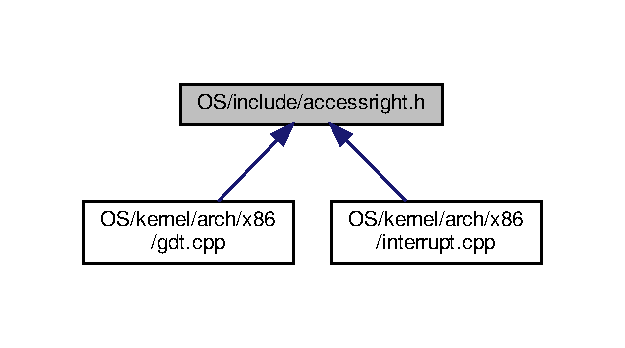
\includegraphics[width=300pt]{accessright_8h__dep__incl}
\end{center}
\end{figure}
\subsection*{Namespaces}
\begin{DoxyCompactItemize}
\item 
 \hyperlink{namespace_a_r}{AR}
\end{DoxyCompactItemize}
\subsection*{Variables}
\begin{DoxyCompactItemize}
\item 
const uint8\+\_\+t \hyperlink{namespace_a_r_a5441c70c25fc8a59482c6b49eb5263fd}{A\+R\+::\+N\+U\+L\+L\+\_\+\+A\+C\+C\+E\+SS} = 0x00
\item 
const uint8\+\_\+t \hyperlink{namespace_a_r_a522bab0f6835eb217d6da7dc243cb321}{A\+R\+::\+K\+E\+R\+N\+\_\+\+C\+S\+\_\+\+A\+C\+C\+E\+SS} = 0x9A
\item 
const uint8\+\_\+t \hyperlink{namespace_a_r_af35b80337e742e9605c8b3a863889545}{A\+R\+::\+U\+S\+E\+R\+\_\+\+C\+S\+\_\+\+A\+C\+C\+E\+SS} = 0x\+FA
\item 
const uint8\+\_\+t \hyperlink{namespace_a_r_adc3973813b32aa819be54d431f1bdb24}{A\+R\+::\+K\+E\+R\+N\+\_\+\+D\+S\+\_\+\+A\+C\+C\+E\+SS} = 0x92
\item 
const uint8\+\_\+t \hyperlink{namespace_a_r_a1b8796b06b020a1610233d041b60e101}{A\+R\+::\+U\+S\+E\+R\+\_\+\+D\+S\+\_\+\+A\+C\+C\+E\+SS} = 0x\+F2
\item 
const uint8\+\_\+t \hyperlink{namespace_a_r_a22cf15841ad21a98049a02bf139f5d90}{A\+R\+::\+I\+N\+T\+E\+R\+R\+U\+P\+T\+\_\+\+A\+C\+C\+E\+SS} = 0x8E
\end{DoxyCompactItemize}

\hypertarget{common_8h}{}\section{O\+S/include/common.h File Reference}
\label{common_8h}\index{O\+S/include/common.\+h@{O\+S/include/common.\+h}}
{\ttfamily \#include $<$stdbool.\+h$>$}\newline
{\ttfamily \#include $<$stddef.\+h$>$}\newline
{\ttfamily \#include $<$stdint.\+h$>$}\newline
{\ttfamily \#include $<$ktypes.\+h$>$}\newline
Include dependency graph for common.\+h\+:\nopagebreak
\begin{figure}[H]
\begin{center}
\leavevmode
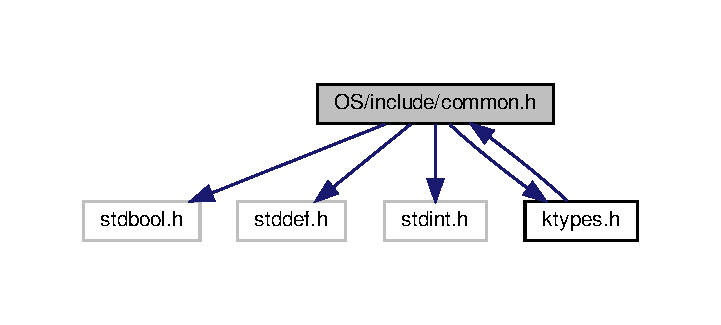
\includegraphics[width=346pt]{common_8h__incl}
\end{center}
\end{figure}
This graph shows which files directly or indirectly include this file\+:\nopagebreak
\begin{figure}[H]
\begin{center}
\leavevmode
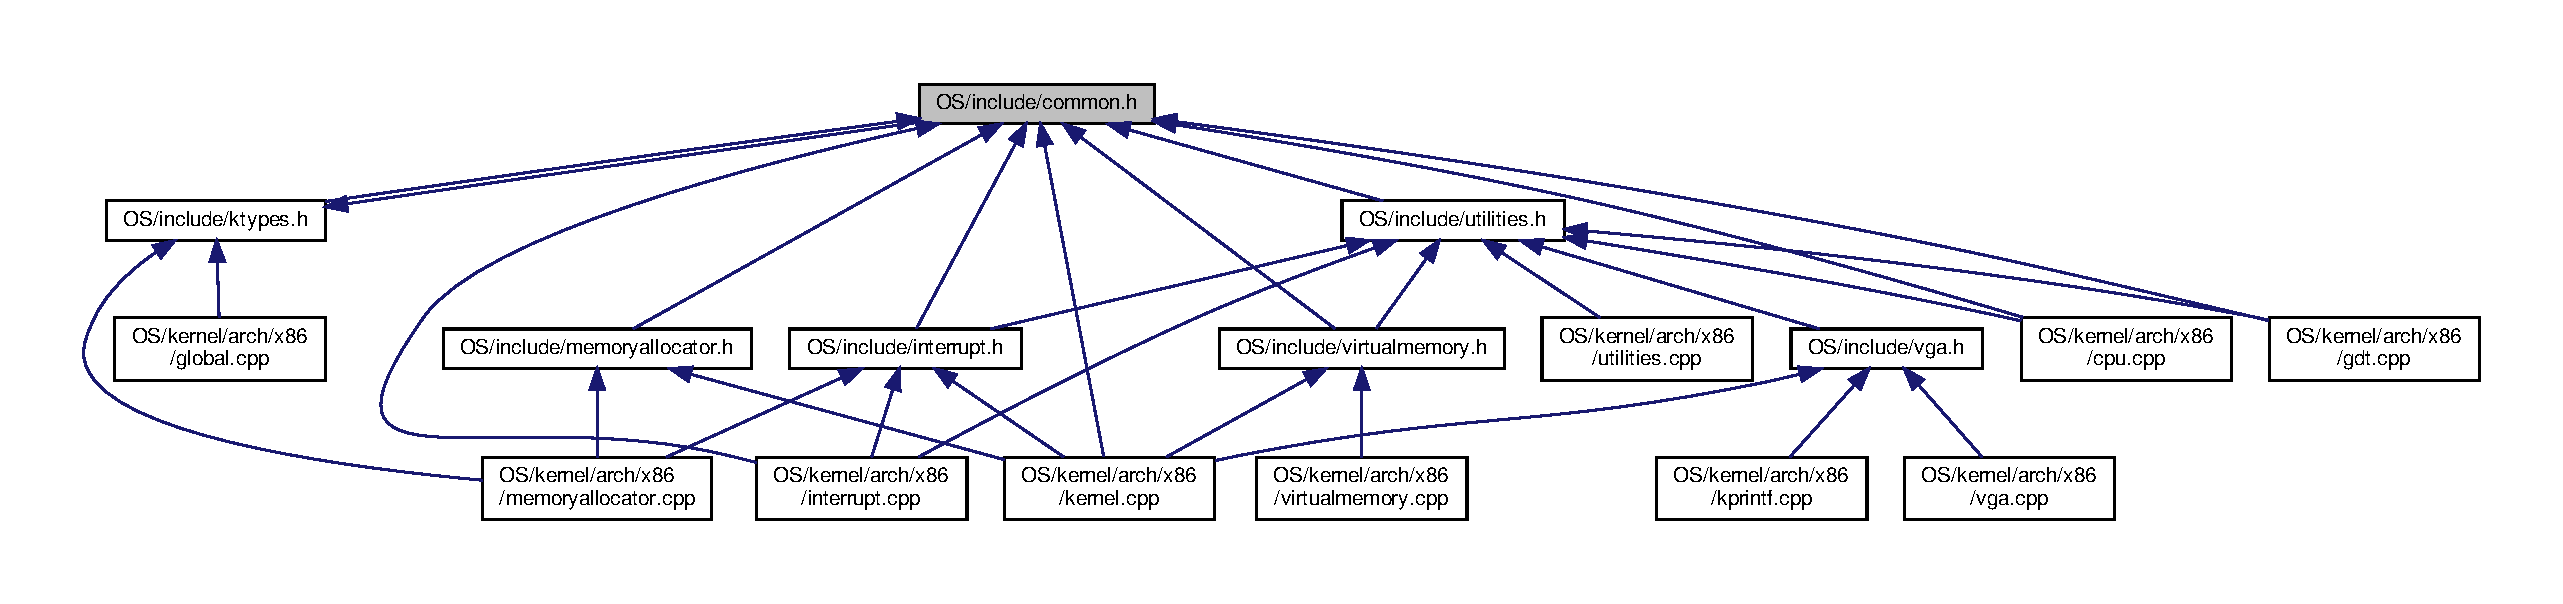
\includegraphics[width=350pt]{common_8h__dep__incl}
\end{center}
\end{figure}

\hypertarget{cpu_8h}{}\section{O\+S/include/cpu.h File Reference}
\label{cpu_8h}\index{O\+S/include/cpu.\+h@{O\+S/include/cpu.\+h}}
This graph shows which files directly or indirectly include this file\+:
\nopagebreak
\begin{figure}[H]
\begin{center}
\leavevmode
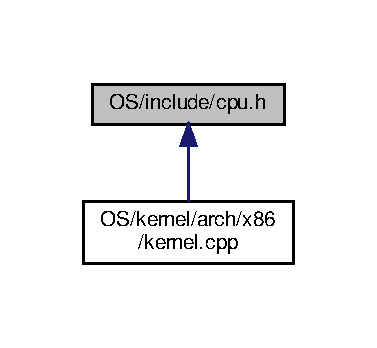
\includegraphics[width=181pt]{cpu_8h__dep__incl}
\end{center}
\end{figure}
\subsection*{Namespaces}
\begin{DoxyCompactItemize}
\item 
 \hyperlink{namespace_i_n_i_t}{I\+N\+IT}
\end{DoxyCompactItemize}
\subsection*{Functions}
\begin{DoxyCompactItemize}
\item 
void \hyperlink{namespace_i_n_i_t_a8928ddbb4ca671dfe1c740da380fa0c4}{I\+N\+I\+T\+::\+S\+SE} ()
\end{DoxyCompactItemize}

\hypertarget{gdt_8h}{}\section{O\+S/include/gdt.h File Reference}
\label{gdt_8h}\index{O\+S/include/gdt.\+h@{O\+S/include/gdt.\+h}}
This graph shows which files directly or indirectly include this file\+:
\nopagebreak
\begin{figure}[H]
\begin{center}
\leavevmode
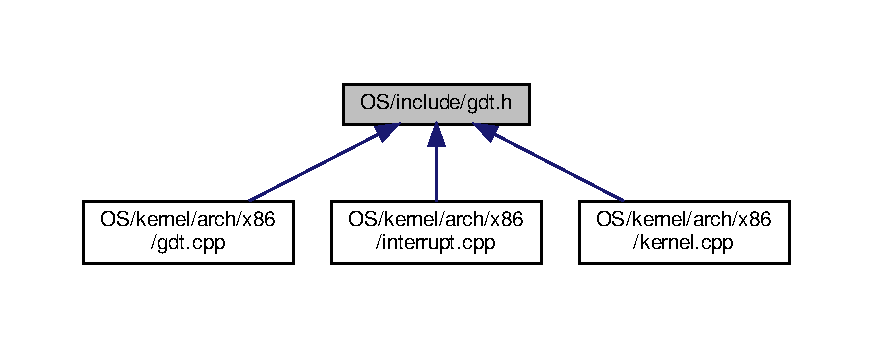
\includegraphics[width=350pt]{gdt_8h__dep__incl}
\end{center}
\end{figure}
\subsection*{Namespaces}
\begin{DoxyCompactItemize}
\item 
 \hyperlink{namespace_g_d_t}{G\+DT}
\item 
 \hyperlink{namespace_i_n_i_t}{I\+N\+IT}
\end{DoxyCompactItemize}
\subsection*{Enumerations}
\begin{DoxyCompactItemize}
\item 
enum \hyperlink{namespace_g_d_t_af2b09941ee46a489ebaccfed5c839154}{G\+D\+T\+::\+Segment} \+: uint16\+\_\+t \{ \newline
\hyperlink{namespace_g_d_t_af2b09941ee46a489ebaccfed5c839154a86e32c8df1a16bdd2971d97063048cff}{G\+D\+T\+::\+Null} = 0, 
\hyperlink{namespace_g_d_t_af2b09941ee46a489ebaccfed5c839154a9ec147ba7f4244a0e047c92f24a920b9}{G\+D\+T\+::\+K\+\_\+\+CS}, 
\hyperlink{namespace_g_d_t_af2b09941ee46a489ebaccfed5c839154a71647052ea8761e0f719dfb481a72f0b}{G\+D\+T\+::\+K\+\_\+\+DS}, 
\hyperlink{namespace_g_d_t_af2b09941ee46a489ebaccfed5c839154a1d5e8e72d040439207b2341afb78e530}{G\+D\+T\+::\+U\+\_\+\+CS}, 
\newline
\hyperlink{namespace_g_d_t_af2b09941ee46a489ebaccfed5c839154a62f547535bd854846bc3d457a3f37eeb}{G\+D\+T\+::\+U\+\_\+\+DS}
 \}
\end{DoxyCompactItemize}
\subsection*{Functions}
\begin{DoxyCompactItemize}
\item 
constexpr uint8\+\_\+t \hyperlink{namespace_g_d_t_a3f6672477fedb061897f9c710f539ccb}{G\+D\+T\+::\+S\+E\+G\+\_\+\+O\+F\+F\+S\+ET} (const Segment Seg)
\item 
void \hyperlink{namespace_i_n_i_t_a3462d7bc51bce77cc240d05b62b1b777}{I\+N\+I\+T\+::gdt} ()
\end{DoxyCompactItemize}
\subsection*{Variables}
\begin{DoxyCompactItemize}
\item 
const uint8\+\_\+t \hyperlink{namespace_g_d_t_aab056cef2c3ca53ed66a58f7ae7edfce}{G\+D\+T\+::\+G\+D\+T\+\_\+\+E\+N\+T\+R\+I\+ES} = 5
\end{DoxyCompactItemize}

\hypertarget{global_8h}{}\section{O\+S/include/global.h File Reference}
\label{global_8h}\index{O\+S/include/global.\+h@{O\+S/include/global.\+h}}
This graph shows which files directly or indirectly include this file\+:
\nopagebreak
\begin{figure}[H]
\begin{center}
\leavevmode
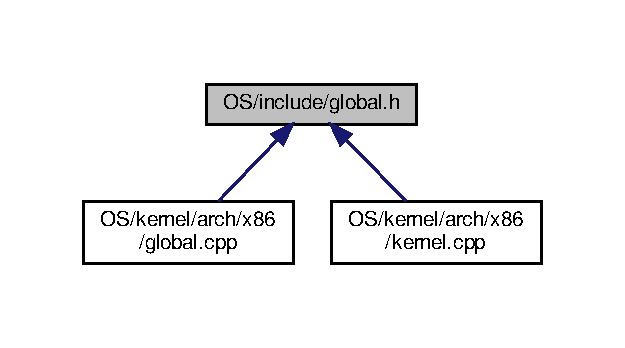
\includegraphics[width=300pt]{global_8h__dep__incl}
\end{center}
\end{figure}
\subsection*{Namespaces}
\begin{DoxyCompactItemize}
\item 
 \hyperlink{namespace_i_n_i_t}{I\+N\+IT}
\end{DoxyCompactItemize}
\subsection*{Functions}
\begin{DoxyCompactItemize}
\item 
void \hyperlink{namespace_i_n_i_t_a6608557e41ad37cdb4a408e2f05c9783}{I\+N\+I\+T\+::ctors} ()
\end{DoxyCompactItemize}

\hypertarget{interrupt_8h}{}\section{O\+S/include/interrupt.h File Reference}
\label{interrupt_8h}\index{O\+S/include/interrupt.\+h@{O\+S/include/interrupt.\+h}}
{\ttfamily \#include $<$common.\+h$>$}\newline
{\ttfamily \#include $<$utilities.\+h$>$}\newline
{\ttfamily \#include $<$registers.\+h$>$}\newline
{\ttfamily \#include $<$ports.\+h$>$}\newline
{\ttfamily \#include $<$pic.\+h$>$}\newline
Include dependency graph for interrupt.\+h\+:
\nopagebreak
\begin{figure}[H]
\begin{center}
\leavevmode
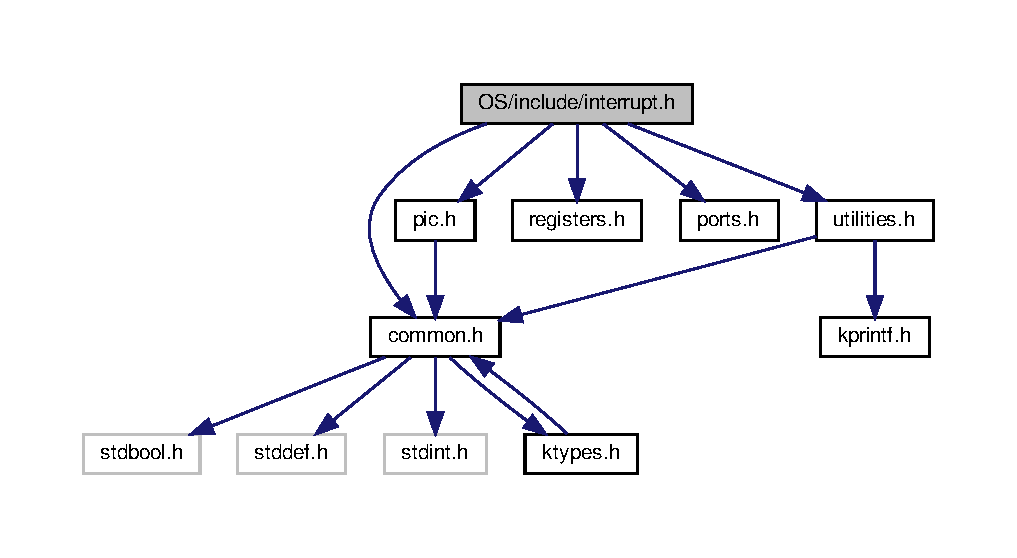
\includegraphics[width=350pt]{interrupt_8h__incl}
\end{center}
\end{figure}
This graph shows which files directly or indirectly include this file\+:
\nopagebreak
\begin{figure}[H]
\begin{center}
\leavevmode
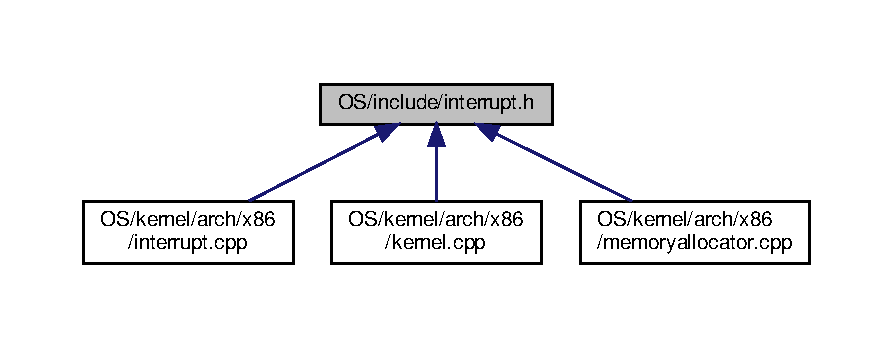
\includegraphics[width=350pt]{interrupt_8h__dep__incl}
\end{center}
\end{figure}
\subsection*{Classes}
\begin{DoxyCompactItemize}
\item 
union \hyperlink{union_i_n_t_r_p_1_1_descriptor_entry}{I\+N\+T\+R\+P\+::\+Descriptor\+Entry}
\begin{DoxyCompactList}\small\item\em Exception and interrupt gate descriptor entry. \end{DoxyCompactList}\item 
class \hyperlink{class_i_n_t_r_p_1_1_mask}{I\+N\+T\+R\+P\+::\+Mask}
\begin{DoxyCompactList}\small\item\em Disables interrupt on construction, restores previous interrupt mask on scope exit. \end{DoxyCompactList}\item 
struct \hyperlink{struct_irq_port}{Irq\+Port}
\item 
class \hyperlink{class_i_r_q_scope}{I\+R\+Q\+Scope}
\end{DoxyCompactItemize}
\subsection*{Namespaces}
\begin{DoxyCompactItemize}
\item 
 \hyperlink{namespace_i_n_t_r_p}{I\+N\+T\+RP}
\begin{DoxyCompactList}\small\item\em interrupt namespace \end{DoxyCompactList}\item 
 \hyperlink{namespace_i_n_i_t}{I\+N\+IT}
\begin{DoxyCompactList}\small\item\em contains all kernel initialization routines \end{DoxyCompactList}\end{DoxyCompactItemize}
\subsection*{Enumerations}
\begin{DoxyCompactItemize}
\item 
enum \hyperlink{namespace_i_n_t_r_p_a790699fb2953ef4ab70c7dc7148a1c94}{I\+N\+T\+R\+P\+::\+I\+VT} \+: uint8\+\_\+t \{ \newline
\hyperlink{namespace_i_n_t_r_p_a790699fb2953ef4ab70c7dc7148a1c94a58f4b58ae6281e7599c8cf5eecb34aac}{I\+N\+T\+R\+P\+::\+R\+E\+S\+E\+R\+V\+E\+D\+\_\+\+S\+T\+A\+RT} = 0x0, 
\hyperlink{namespace_i_n_t_r_p_a790699fb2953ef4ab70c7dc7148a1c94aa4812872ae63e8dd2531baae7ae7af8c}{I\+N\+T\+R\+P\+::\+D\+I\+V\+\_\+0\+\_\+\+F\+A\+U\+LT} = R\+E\+S\+E\+R\+V\+E\+D\+\_\+\+S\+T\+A\+RT, 
\hyperlink{namespace_i_n_t_r_p_a790699fb2953ef4ab70c7dc7148a1c94a3e90a0065c250e74b2e79839e6dd9531}{I\+N\+T\+R\+P\+::\+D\+E\+B\+U\+G\+\_\+\+T\+R\+AP} = 0x1, 
\hyperlink{namespace_i_n_t_r_p_a790699fb2953ef4ab70c7dc7148a1c94a60c43a2567dc9655eac98fe90703e4e4}{I\+N\+T\+R\+P\+::\+N\+M\+I\+\_\+\+I\+N\+T\+E\+R\+R\+U\+PT} = 0x2, 
\newline
\hyperlink{namespace_i_n_t_r_p_a790699fb2953ef4ab70c7dc7148a1c94ac40b8e367b8789ee9a9138c7e5c5e7b9}{I\+N\+T\+R\+P\+::\+B\+R\+E\+A\+K\+P\+O\+I\+N\+T\+\_\+\+T\+R\+AP} = 0x3, 
\hyperlink{namespace_i_n_t_r_p_a790699fb2953ef4ab70c7dc7148a1c94a6bf9679b51b0ae4fc7d0b89b62ae19c2}{I\+N\+T\+R\+P\+::\+O\+V\+E\+R\+F\+L\+O\+W\+\_\+\+T\+R\+AP} = 0x4, 
\hyperlink{namespace_i_n_t_r_p_a790699fb2953ef4ab70c7dc7148a1c94aecc41fcce90166e7c060af4df3eb85e9}{I\+N\+T\+R\+P\+::\+O\+U\+T\+\_\+\+O\+F\+\_\+\+B\+O\+U\+N\+D\+S\+\_\+\+F\+A\+U\+LT} = 0x5, 
\hyperlink{namespace_i_n_t_r_p_a790699fb2953ef4ab70c7dc7148a1c94af5e5df39002d4114a23ea47772b24993}{I\+N\+T\+R\+P\+::\+I\+N\+V\+A\+L\+I\+D\+\_\+\+O\+P\+C\+O\+D\+E\+\_\+\+F\+A\+U\+LT} = 0x6, 
\newline
\hyperlink{namespace_i_n_t_r_p_a790699fb2953ef4ab70c7dc7148a1c94a917bad20e5e7152140c3bc4a32f0c946}{I\+N\+T\+R\+P\+::\+N\+O\+\_\+\+M\+A\+T\+H\+\_\+\+C\+O\+P\+\_\+\+F\+A\+U\+LT} = 0x7, 
\hyperlink{namespace_i_n_t_r_p_a790699fb2953ef4ab70c7dc7148a1c94a4dc8cc2535405b9892ebb823cc708724}{I\+N\+T\+R\+P\+::\+D\+O\+U\+B\+L\+E\+\_\+\+F\+A\+U\+LT} = 0x8, 
\hyperlink{namespace_i_n_t_r_p_a790699fb2953ef4ab70c7dc7148a1c94a777235d584c5919bd2b1ce4f436515bd}{I\+N\+T\+R\+P\+::\+C\+O\+P\+\_\+\+S\+E\+G\+\_\+\+O\+V\+E\+R\+R\+U\+N\+\_\+\+F\+A\+U\+LT} = 0x9, 
\hyperlink{namespace_i_n_t_r_p_a790699fb2953ef4ab70c7dc7148a1c94a5b1eba48c3b793f1335078cd5231f50d}{I\+N\+T\+R\+P\+::\+I\+N\+V\+A\+L\+I\+D\+\_\+\+T\+S\+S\+\_\+\+F\+A\+U\+LT} = 0x0A, 
\newline
\hyperlink{namespace_i_n_t_r_p_a790699fb2953ef4ab70c7dc7148a1c94a654096aa14bd7f00822273e7fe86525f}{I\+N\+T\+R\+P\+::\+S\+E\+G\+\_\+\+N\+O\+T\+\_\+\+P\+R\+E\+S\+E\+N\+T\+\_\+\+F\+A\+U\+LT} = 0x0B, 
\hyperlink{namespace_i_n_t_r_p_a790699fb2953ef4ab70c7dc7148a1c94aa151e7e1c98c688471f4e9b60fd11de9}{I\+N\+T\+R\+P\+::\+S\+T\+A\+C\+K\+\_\+\+S\+E\+G\+\_\+\+F\+A\+U\+LT} = 0x0C, 
\hyperlink{namespace_i_n_t_r_p_a790699fb2953ef4ab70c7dc7148a1c94a2494cab6d93c57a9adcb3d7309192b79}{I\+N\+T\+R\+P\+::\+G\+E\+N\+\_\+\+P\+R\+O\+T\+E\+C\+T\+I\+O\+N\+\_\+\+F\+A\+U\+LT} = 0x0D, 
\hyperlink{namespace_i_n_t_r_p_a790699fb2953ef4ab70c7dc7148a1c94a72999410be9f8206ea01268b6306f59a}{I\+N\+T\+R\+P\+::\+P\+A\+G\+E\+\_\+\+F\+A\+U\+LT} = 0x0E, 
\newline
\hyperlink{namespace_i_n_t_r_p_a790699fb2953ef4ab70c7dc7148a1c94a24b3949bacfadc75ecddaf0a638b1c49}{I\+N\+T\+R\+P\+::\+R\+E\+S\+E\+R\+V\+ED} = 0x0F, 
\hyperlink{namespace_i_n_t_r_p_a790699fb2953ef4ab70c7dc7148a1c94a44642a04b137a14fd789a6936b7762dd}{I\+N\+T\+R\+P\+::\+M\+A\+T\+H\+\_\+\+F\+A\+U\+LT} = 0x10, 
\hyperlink{namespace_i_n_t_r_p_a790699fb2953ef4ab70c7dc7148a1c94a4ae4571bf9290f732b429dd0b30002c3}{I\+N\+T\+R\+P\+::\+A\+L\+I\+G\+N\+M\+E\+N\+T\+\_\+\+C\+H\+E\+C\+K\+\_\+\+F\+A\+U\+LT} = 0x11, 
\hyperlink{namespace_i_n_t_r_p_a790699fb2953ef4ab70c7dc7148a1c94a67d00b54b2bade5a703dbbbc2ea93711}{I\+N\+T\+R\+P\+::\+M\+A\+C\+H\+I\+N\+E\+\_\+\+C\+H\+E\+C\+K\+\_\+\+A\+B\+O\+RT} = 0x12, 
\newline
\hyperlink{namespace_i_n_t_r_p_a790699fb2953ef4ab70c7dc7148a1c94a7f928e26348ad94a198cdb0b8758068b}{I\+N\+T\+R\+P\+::\+S\+I\+M\+D\+\_\+\+F\+P\+\_\+\+X\+F\+\_\+\+F\+A\+U\+LT} = 0x13, 
\hyperlink{namespace_i_n_t_r_p_a790699fb2953ef4ab70c7dc7148a1c94ad3c957dd69dc16828a748d3e07499633}{I\+N\+T\+R\+P\+::\+R\+E\+S\+E\+R\+V\+E\+D\+\_\+\+E\+ND} = 0x1F, 
\hyperlink{namespace_i_n_t_r_p_a790699fb2953ef4ab70c7dc7148a1c94aeab865c11d738ea404326f4999d931a4}{I\+N\+T\+R\+P\+::\+P\+I\+C1\+\_\+\+O\+F\+F\+S\+ET} = 0x20, 
\hyperlink{namespace_i_n_t_r_p_a790699fb2953ef4ab70c7dc7148a1c94a6896b72dca7a4ffbd39151b6fb9be9b1}{I\+N\+T\+R\+P\+::\+U\+S\+E\+R\+\_\+\+D\+E\+F\+I\+N\+E\+D\+\_\+\+S\+T\+A\+RT} = P\+I\+C1\+\_\+\+O\+F\+F\+S\+ET, 
\newline
\hyperlink{namespace_i_n_t_r_p_a790699fb2953ef4ab70c7dc7148a1c94af70d004a23c393fec49b90824737a388}{I\+N\+T\+R\+P\+::\+T\+I\+M\+ER} = 0x20, 
\hyperlink{namespace_i_n_t_r_p_a790699fb2953ef4ab70c7dc7148a1c94a26c910d31696aaa9f143858c1ca8f88a}{I\+N\+T\+R\+P\+::\+K\+E\+Y\+B\+O\+A\+RD} = 0x21, 
\hyperlink{namespace_i_n_t_r_p_a790699fb2953ef4ab70c7dc7148a1c94a8ff3a4bd7727d04134803c16480a7fad}{I\+N\+T\+R\+P\+::\+P\+I\+C2\+\_\+\+C\+A\+S\+C\+A\+DE} = 0x22, 
\hyperlink{namespace_i_n_t_r_p_a790699fb2953ef4ab70c7dc7148a1c94a5a3d86f12fc0a66f036a81b07dec9de8}{I\+N\+T\+R\+P\+::\+S\+E\+R\+I\+A\+L2} = 0x23, 
\newline
\hyperlink{namespace_i_n_t_r_p_a790699fb2953ef4ab70c7dc7148a1c94abd2a8df6358eec4253d4a0007be75f13}{I\+N\+T\+R\+P\+::\+S\+E\+R\+I\+A\+L1} = 0x24, 
\hyperlink{namespace_i_n_t_r_p_a790699fb2953ef4ab70c7dc7148a1c94a78ae5cd5022a6b6c1aea66d4b9925b81}{I\+N\+T\+R\+P\+::\+P\+A\+R\+A\+L\+L\+E\+L2} = 0x25, 
\hyperlink{namespace_i_n_t_r_p_a790699fb2953ef4ab70c7dc7148a1c94a1518e23a795c53f82e8256929c0ad5af}{I\+N\+T\+R\+P\+::\+D\+I\+S\+K\+E\+T\+TE} = 0x26, 
\hyperlink{namespace_i_n_t_r_p_a790699fb2953ef4ab70c7dc7148a1c94ab2cb88c7d3a471aceb60e48b46c6280e}{I\+N\+T\+R\+P\+::\+P\+A\+R\+A\+L\+L\+E\+L1} = 0x27, 
\newline
\hyperlink{namespace_i_n_t_r_p_a790699fb2953ef4ab70c7dc7148a1c94a7bf9df9e133a0dc85c31c1e83b0e4583}{I\+N\+T\+R\+P\+::\+P\+I\+C2\+\_\+\+O\+F\+F\+S\+ET} = 0x28, 
\hyperlink{namespace_i_n_t_r_p_a790699fb2953ef4ab70c7dc7148a1c94a7845705230fa4742fe60b758a7348bf5}{I\+N\+T\+R\+P\+::\+C\+M\+OS} = 0x28, 
\hyperlink{namespace_i_n_t_r_p_a790699fb2953ef4ab70c7dc7148a1c94ab587d9eed26df4e7f9055743d23725a0}{I\+N\+T\+R\+P\+::\+C\+GA} = 0x29, 
\hyperlink{namespace_i_n_t_r_p_a790699fb2953ef4ab70c7dc7148a1c94a5bb3ea184473d7cfe02ba66cd25b7e2e}{I\+N\+T\+R\+P\+::\+R\+E\+S\+E\+R\+V\+E\+D1} = 0x2A, 
\newline
\hyperlink{namespace_i_n_t_r_p_a790699fb2953ef4ab70c7dc7148a1c94a502440134aaf6ca0554d46c5afefdbd5}{I\+N\+T\+R\+P\+::\+R\+E\+S\+E\+R\+V\+E\+D2} = 0x2B, 
\hyperlink{namespace_i_n_t_r_p_a790699fb2953ef4ab70c7dc7148a1c94a69b1631499d394b6dcc6835f0f992a71}{I\+N\+T\+R\+P\+::\+P\+S2} = 0x2C, 
\hyperlink{namespace_i_n_t_r_p_a790699fb2953ef4ab70c7dc7148a1c94a126c5a0df859ba26819002a933954668}{I\+N\+T\+R\+P\+::\+F\+PU} = 0x2D, 
\hyperlink{namespace_i_n_t_r_p_a790699fb2953ef4ab70c7dc7148a1c94a5f2afad82b6da16473d3954a3448f0f0}{I\+N\+T\+R\+P\+::\+H\+A\+R\+D\+D\+I\+SK} = 0x2E, 
\newline
\hyperlink{namespace_i_n_t_r_p_a790699fb2953ef4ab70c7dc7148a1c94a0fe0125f905bc4888ffddb4b791fd30e}{I\+N\+T\+R\+P\+::\+R\+E\+S\+E\+R\+V\+E\+D3} = 0x2F, 
\hyperlink{namespace_i_n_t_r_p_a790699fb2953ef4ab70c7dc7148a1c94ae081b819aecf9800dc041fec2b47286c}{I\+N\+T\+R\+P\+::\+U\+S\+E\+R\+\_\+\+D\+E\+F\+I\+N\+E\+D\+\_\+\+E\+ND} = 0x\+FF
 \}
\end{DoxyCompactItemize}
\subsection*{Functions}
\begin{DoxyCompactItemize}
\item 
void \hyperlink{namespace_i_n_t_r_p_a91a6a2668bfa9961a9ed265f6ceac47d}{I\+N\+T\+R\+P\+::\+Register\+Handler} (Descriptor\+Entry Idt\+Table\mbox{[}$\,$\mbox{]}, size\+\_\+t Idx, \hyperlink{ktypes_8h_a46bbb9e776183ed6a8eca9d919756434}{func\+\_\+ptr} Handler)
\begin{DoxyCompactList}\small\item\em Creates interrupt descriptor entries in idt\+\_\+table, and loads into C\+PU. \end{DoxyCompactList}\item 
void \hyperlink{interrupt_8h_adf606426a25a7b6b549ad9a97c2e04b8}{Unmask\+Interrupt} (const \hyperlink{struct_irq_port}{Irq\+Port} Irq)
\item 
void \hyperlink{namespace_i_n_i_t_aec8e9f01cb09653075b6e610096b3ca9}{I\+N\+I\+T\+::idt} ()
\begin{DoxyCompactList}\small\item\em Creates interrupt descriptor table and loads to C\+PU. \end{DoxyCompactList}\end{DoxyCompactItemize}
\subsection*{Variables}
\begin{DoxyCompactItemize}
\item 
const uint16\+\_\+t \hyperlink{namespace_i_n_t_r_p_a1022b4dc1d9af1ea393f7f038ff421ce}{I\+N\+T\+R\+P\+::\+I\+D\+T\+\_\+\+E\+N\+T\+R\+I\+ES} = 256
\end{DoxyCompactItemize}


\subsection{Function Documentation}
\mbox{\Hypertarget{interrupt_8h_adf606426a25a7b6b549ad9a97c2e04b8}\label{interrupt_8h_adf606426a25a7b6b549ad9a97c2e04b8}} 
\index{interrupt.\+h@{interrupt.\+h}!Unmask\+Interrupt@{Unmask\+Interrupt}}
\index{Unmask\+Interrupt@{Unmask\+Interrupt}!interrupt.\+h@{interrupt.\+h}}
\subsubsection{\texorpdfstring{Unmask\+Interrupt()}{UnmaskInterrupt()}}
{\footnotesize\ttfamily void Unmask\+Interrupt (\begin{DoxyParamCaption}\item[{const \hyperlink{struct_irq_port}{Irq\+Port}}]{Irq }\end{DoxyParamCaption})\hspace{0.3cm}{\ttfamily [inline]}}



Definition at line 156 of file interrupt.\+h.


\hypertarget{kprintf_8h}{}\section{O\+S/include/kprintf.h File Reference}
\label{kprintf_8h}\index{O\+S/include/kprintf.\+h@{O\+S/include/kprintf.\+h}}
This graph shows which files directly or indirectly include this file\+:
\nopagebreak
\begin{figure}[H]
\begin{center}
\leavevmode
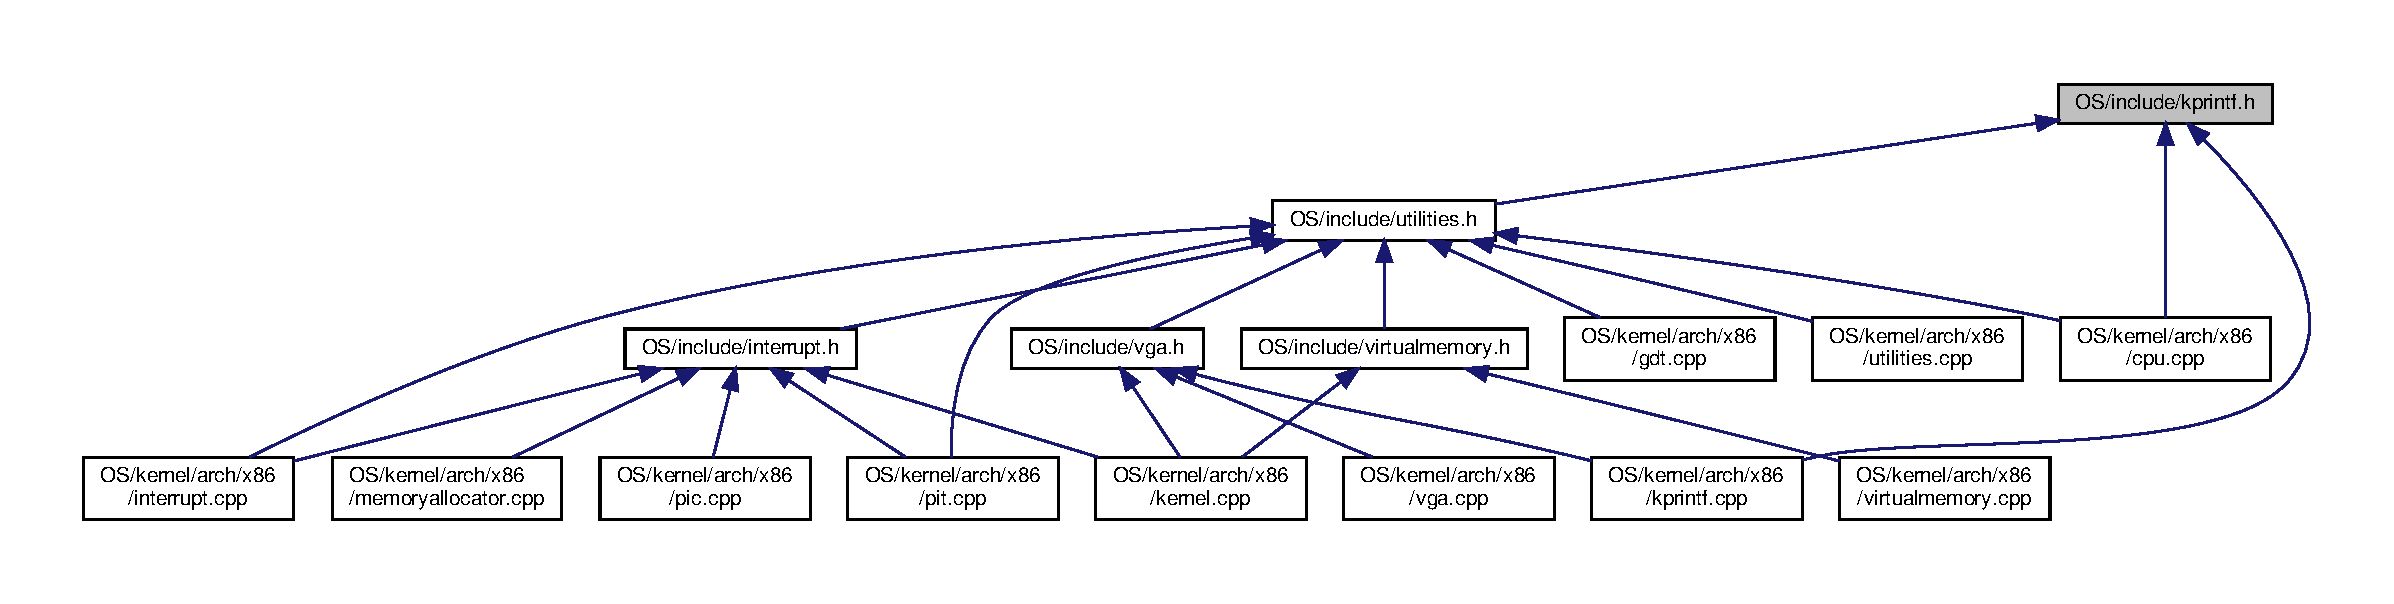
\includegraphics[width=350pt]{kprintf_8h__dep__incl}
\end{center}
\end{figure}
\subsection*{Functions}
\begin{DoxyCompactItemize}
\item 
void \hyperlink{kprintf_8h_ae610f6b2bc90ea3eed7852d591c48116}{kprintf} (const char $\ast$Str)
\begin{DoxyCompactList}\small\item\em Prints string to display. \end{DoxyCompactList}\end{DoxyCompactItemize}


\subsection{Function Documentation}
\mbox{\Hypertarget{kprintf_8h_ae610f6b2bc90ea3eed7852d591c48116}\label{kprintf_8h_ae610f6b2bc90ea3eed7852d591c48116}} 
\index{kprintf.\+h@{kprintf.\+h}!kprintf@{kprintf}}
\index{kprintf@{kprintf}!kprintf.\+h@{kprintf.\+h}}
\subsubsection{\texorpdfstring{kprintf()}{kprintf()}}
{\footnotesize\ttfamily void kprintf (\begin{DoxyParamCaption}\item[{const char $\ast$}]{Str }\end{DoxyParamCaption})}



Prints string to display. 


\begin{DoxyParams}{Parameters}
{\em Str} & -\/ string to print \\
\hline
\end{DoxyParams}


Definition at line 13 of file kprintf.\+cpp.


\hypertarget{ktypes_8h}{}\section{O\+S/include/ktypes.h File Reference}
\label{ktypes_8h}\index{O\+S/include/ktypes.\+h@{O\+S/include/ktypes.\+h}}
{\ttfamily \#include $<$common.\+h$>$}\newline
Include dependency graph for ktypes.\+h\+:\nopagebreak
\begin{figure}[H]
\begin{center}
\leavevmode
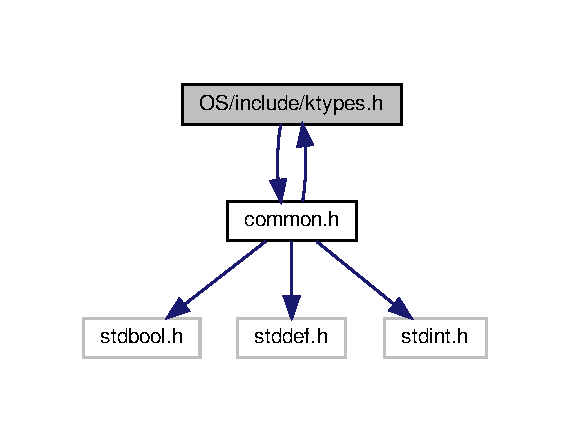
\includegraphics[width=274pt]{ktypes_8h__incl}
\end{center}
\end{figure}
This graph shows which files directly or indirectly include this file\+:\nopagebreak
\begin{figure}[H]
\begin{center}
\leavevmode
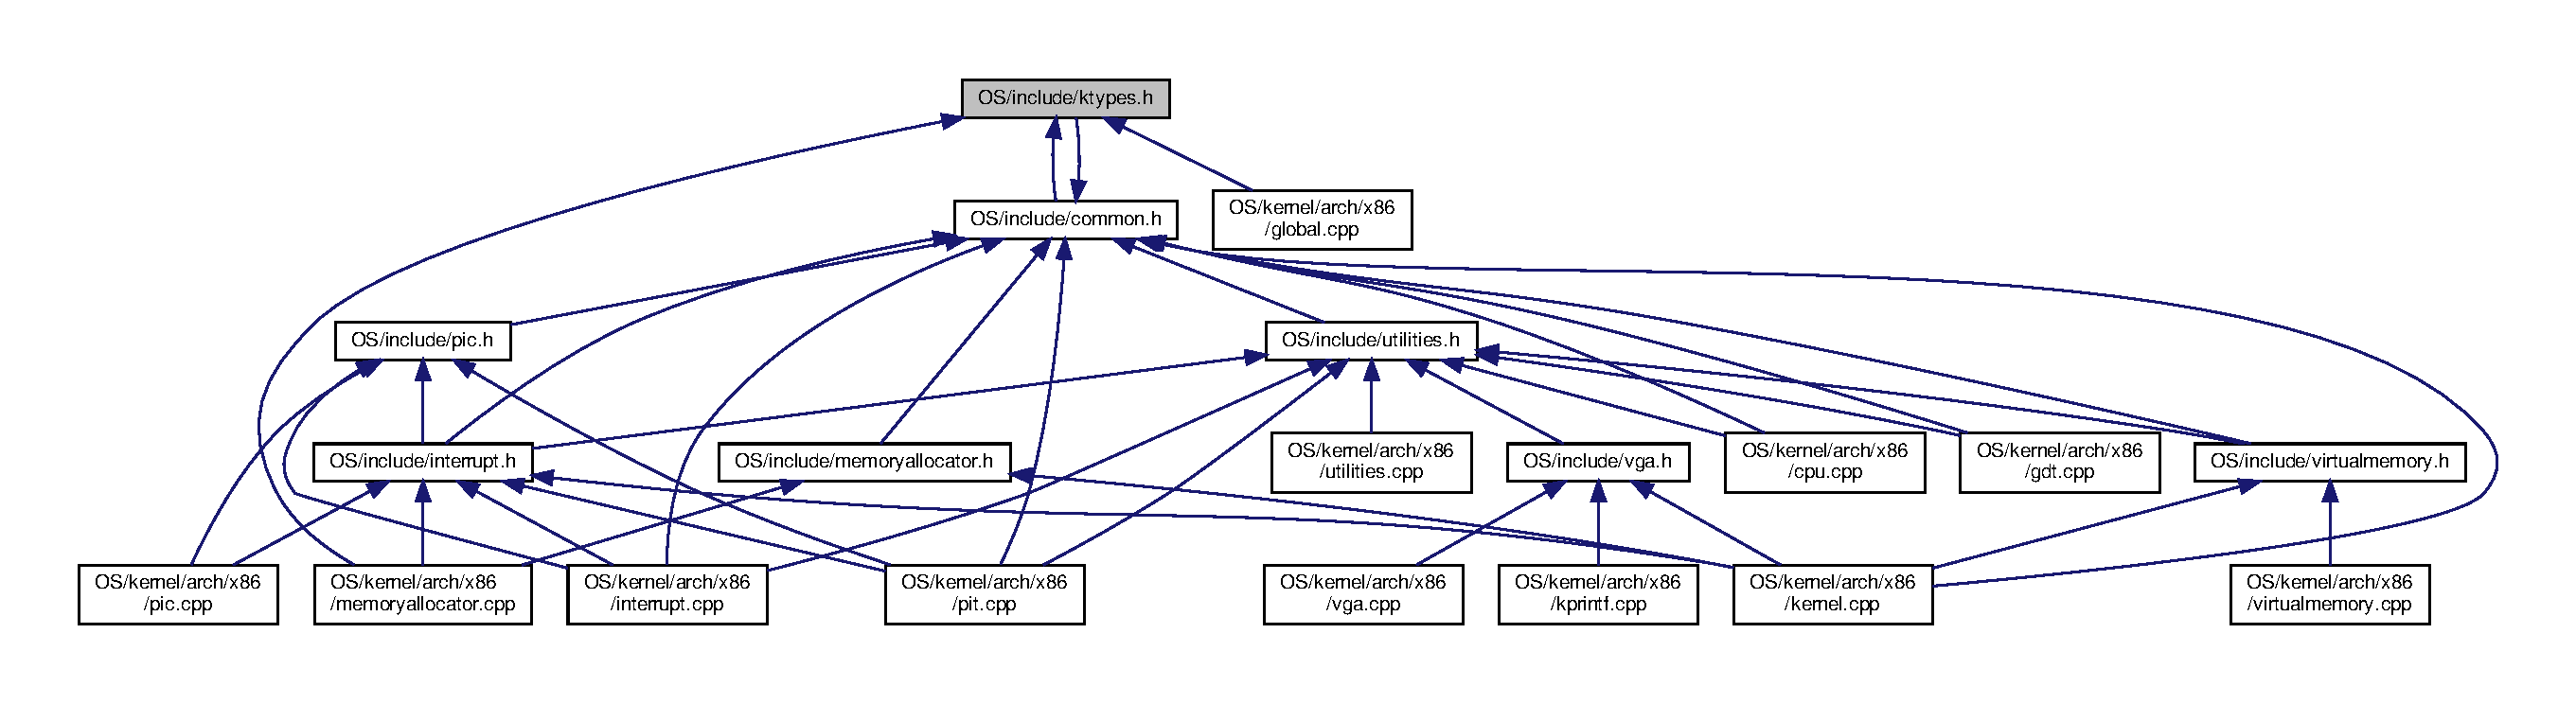
\includegraphics[width=350pt]{ktypes_8h__dep__incl}
\end{center}
\end{figure}
\subsection*{Typedefs}
\begin{DoxyCompactItemize}
\item 
typedef uint64\+\_\+t \hyperlink{ktypes_8h_a3f13e4d5a59d909d6303f569fe5e6524}{ptr\+\_\+t}
\item 
using \hyperlink{ktypes_8h_a46bbb9e776183ed6a8eca9d919756434}{func\+\_\+ptr} = void($\ast$)()
\end{DoxyCompactItemize}
\subsection*{Variables}
\begin{DoxyCompactItemize}
\item 
const uint32\+\_\+t \hyperlink{ktypes_8h_a96706bd96cdf035fc13c13879703c3c4}{S\+Y\+S\+E\+RR} = -\/1
\end{DoxyCompactItemize}


\subsection{Typedef Documentation}
\mbox{\Hypertarget{ktypes_8h_a46bbb9e776183ed6a8eca9d919756434}\label{ktypes_8h_a46bbb9e776183ed6a8eca9d919756434}} 
\index{ktypes.\+h@{ktypes.\+h}!func\+\_\+ptr@{func\+\_\+ptr}}
\index{func\+\_\+ptr@{func\+\_\+ptr}!ktypes.\+h@{ktypes.\+h}}
\subsubsection{\texorpdfstring{func\+\_\+ptr}{func\_ptr}}
{\footnotesize\ttfamily using \hyperlink{ktypes_8h_a46bbb9e776183ed6a8eca9d919756434}{func\+\_\+ptr} =  void($\ast$)()}



Definition at line 16 of file ktypes.\+h.

\mbox{\Hypertarget{ktypes_8h_a3f13e4d5a59d909d6303f569fe5e6524}\label{ktypes_8h_a3f13e4d5a59d909d6303f569fe5e6524}} 
\index{ktypes.\+h@{ktypes.\+h}!ptr\+\_\+t@{ptr\+\_\+t}}
\index{ptr\+\_\+t@{ptr\+\_\+t}!ktypes.\+h@{ktypes.\+h}}
\subsubsection{\texorpdfstring{ptr\+\_\+t}{ptr\_t}}
{\footnotesize\ttfamily typedef uint64\+\_\+t \hyperlink{ktypes_8h_a3f13e4d5a59d909d6303f569fe5e6524}{ptr\+\_\+t}}



Definition at line 13 of file ktypes.\+h.



\subsection{Variable Documentation}
\mbox{\Hypertarget{ktypes_8h_a96706bd96cdf035fc13c13879703c3c4}\label{ktypes_8h_a96706bd96cdf035fc13c13879703c3c4}} 
\index{ktypes.\+h@{ktypes.\+h}!S\+Y\+S\+E\+RR@{S\+Y\+S\+E\+RR}}
\index{S\+Y\+S\+E\+RR@{S\+Y\+S\+E\+RR}!ktypes.\+h@{ktypes.\+h}}
\subsubsection{\texorpdfstring{S\+Y\+S\+E\+RR}{SYSERR}}
{\footnotesize\ttfamily const uint32\+\_\+t S\+Y\+S\+E\+RR = -\/1}



Definition at line 18 of file ktypes.\+h.


\hypertarget{memoryallocator_8h}{}\section{O\+S/include/memoryallocator.h File Reference}
\label{memoryallocator_8h}\index{O\+S/include/memoryallocator.\+h@{O\+S/include/memoryallocator.\+h}}
{\ttfamily \#include $<$common.\+h$>$}\newline
Include dependency graph for memoryallocator.\+h\+:\nopagebreak
\begin{figure}[H]
\begin{center}
\leavevmode
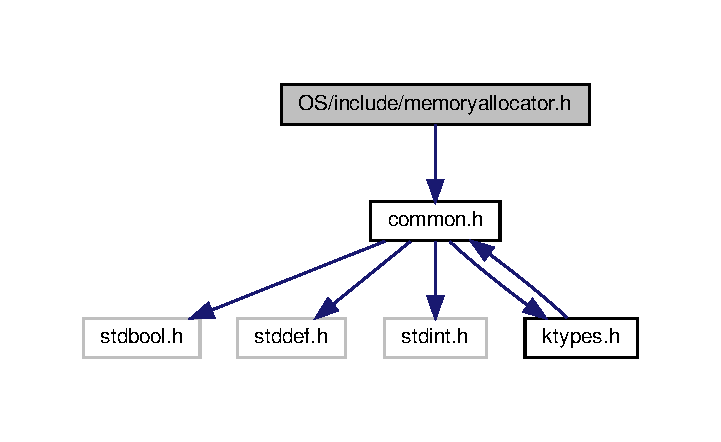
\includegraphics[width=346pt]{memoryallocator_8h__incl}
\end{center}
\end{figure}
This graph shows which files directly or indirectly include this file\+:\nopagebreak
\begin{figure}[H]
\begin{center}
\leavevmode
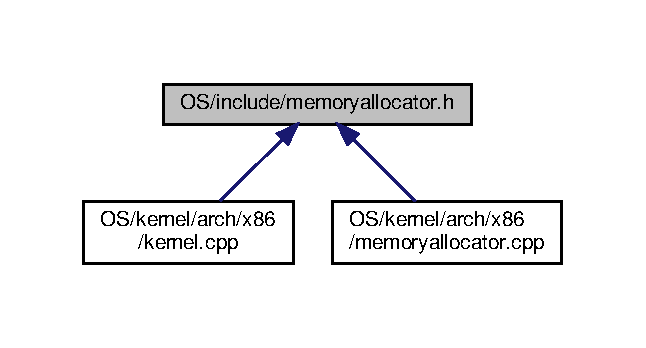
\includegraphics[width=310pt]{memoryallocator_8h__dep__incl}
\end{center}
\end{figure}
\subsection*{Classes}
\begin{DoxyCompactItemize}
\item 
class \hyperlink{class_k_m_1_1_memory_allocator}{K\+M\+::\+Memory\+Allocator}
\begin{DoxyCompactList}\small\item\em Manages kernel heap memory. \end{DoxyCompactList}\end{DoxyCompactItemize}
\subsection*{Namespaces}
\begin{DoxyCompactItemize}
\item 
 \hyperlink{namespace_k_m}{KM}
\begin{DoxyCompactList}\small\item\em Kernel memory namespace. \end{DoxyCompactList}\item 
 \hyperlink{namespace_i_n_i_t}{I\+N\+IT}
\begin{DoxyCompactList}\small\item\em contains all kernel initialization routines \end{DoxyCompactList}\end{DoxyCompactItemize}
\subsection*{Functions}
\begin{DoxyCompactItemize}
\item 
void $\ast$ \hyperlink{namespace_k_m_aaeb8403b430af6311bb3c1df6ae520b6}{K\+M\+::kmalloc} (size\+\_\+t Size)
\begin{DoxyCompactList}\small\item\em kernel malloc \end{DoxyCompactList}\item 
void \hyperlink{namespace_k_m_a08363437a217255f3f9d2a393a54714b}{K\+M\+::free} (void $\ast$Ptr)
\begin{DoxyCompactList}\small\item\em kernel free \end{DoxyCompactList}\item 
void \hyperlink{namespace_i_n_i_t_ac811302ce0948a6a097b445b811f9c14}{I\+N\+I\+T\+::\+K\+M\+A\+L\+L\+OC} ()
\begin{DoxyCompactList}\small\item\em Provides memory allocator with range of reserved memory address to manage. \end{DoxyCompactList}\end{DoxyCompactItemize}
\subsection*{Variables}
\begin{DoxyCompactItemize}
\item 
Memory\+Allocator \hyperlink{namespace_k_m_ab71afb37d9950edf604f583b657905aa}{K\+M\+::mem\+\_\+alloc}
\end{DoxyCompactItemize}

\hypertarget{utilities_8h}{}\section{O\+S/include/utilities.h File Reference}
\label{utilities_8h}\index{O\+S/include/utilities.\+h@{O\+S/include/utilities.\+h}}
{\ttfamily \#include $<$common.\+h$>$}\newline
{\ttfamily \#include $<$kprintf.\+h$>$}\newline
Include dependency graph for utilities.\+h\+:\nopagebreak
\begin{figure}[H]
\begin{center}
\leavevmode
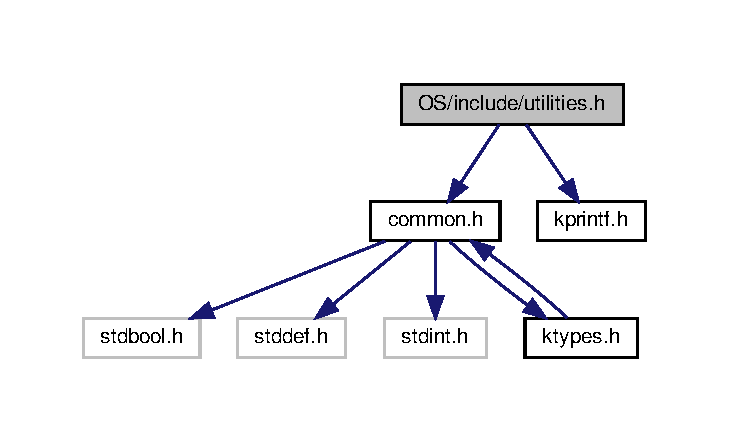
\includegraphics[width=350pt]{utilities_8h__incl}
\end{center}
\end{figure}
This graph shows which files directly or indirectly include this file\+:
\nopagebreak
\begin{figure}[H]
\begin{center}
\leavevmode
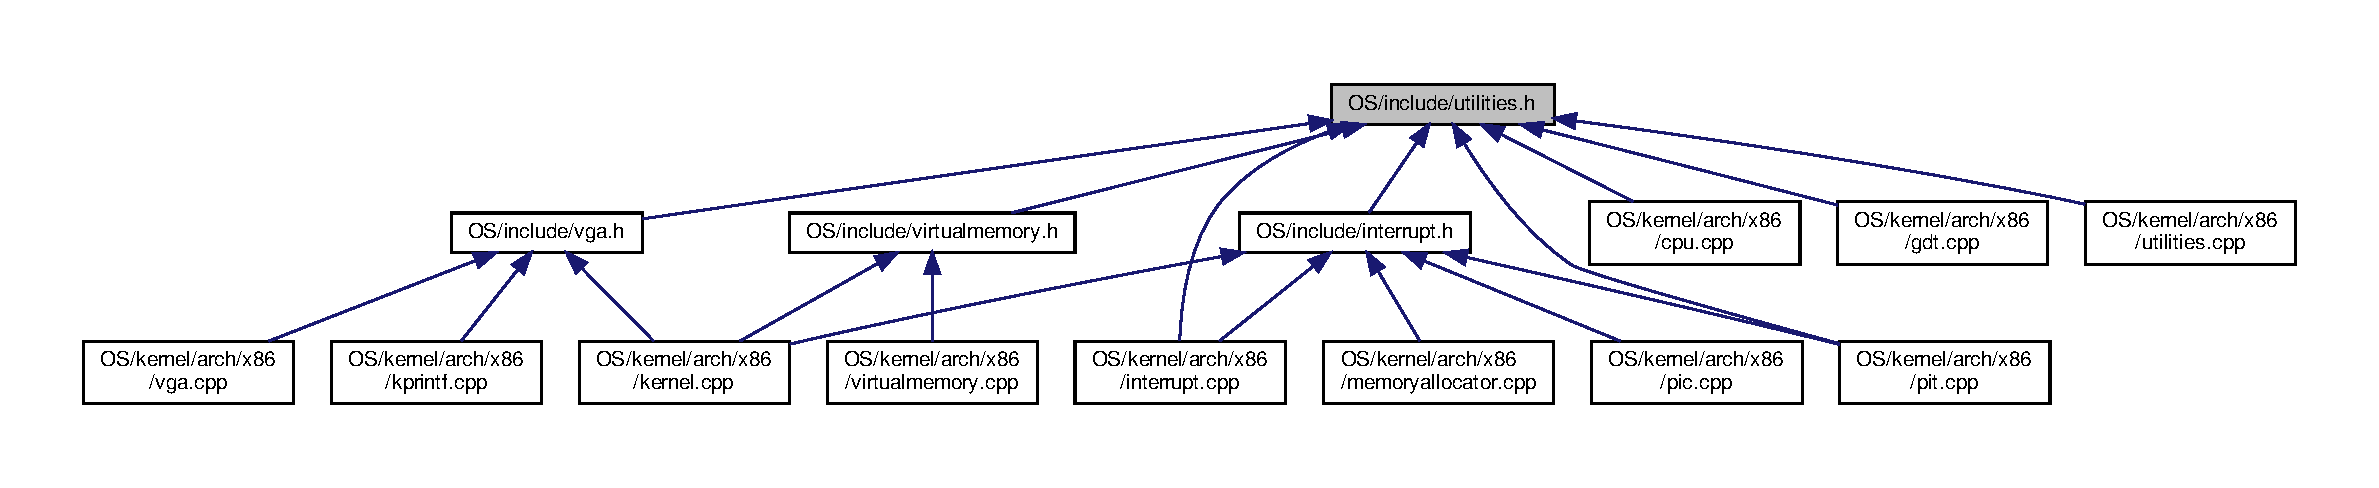
\includegraphics[width=350pt]{utilities_8h__dep__incl}
\end{center}
\end{figure}
\subsection*{Macros}
\begin{DoxyCompactItemize}
\item 
\#define \hyperlink{utilities_8h_ac59ef5882196a6293008a4fc4f97e96c}{G\+H\+E\+T\+T\+O\+\_\+\+G\+E\+T\+\_\+\+CR}(x)
\end{DoxyCompactItemize}
\subsection*{Functions}
\begin{DoxyCompactItemize}
\item 
size\+\_\+t \hyperlink{utilities_8h_a05b27f5e571488d0a74e4bd70b612874}{Strlen} (const char $\ast$Str)
\begin{DoxyCompactList}\small\item\em Count number of characters in string. \end{DoxyCompactList}\end{DoxyCompactItemize}


\subsection{Macro Definition Documentation}
\mbox{\Hypertarget{utilities_8h_ac59ef5882196a6293008a4fc4f97e96c}\label{utilities_8h_ac59ef5882196a6293008a4fc4f97e96c}} 
\index{utilities.\+h@{utilities.\+h}!G\+H\+E\+T\+T\+O\+\_\+\+G\+E\+T\+\_\+\+CR@{G\+H\+E\+T\+T\+O\+\_\+\+G\+E\+T\+\_\+\+CR}}
\index{G\+H\+E\+T\+T\+O\+\_\+\+G\+E\+T\+\_\+\+CR@{G\+H\+E\+T\+T\+O\+\_\+\+G\+E\+T\+\_\+\+CR}!utilities.\+h@{utilities.\+h}}
\subsubsection{\texorpdfstring{G\+H\+E\+T\+T\+O\+\_\+\+G\+E\+T\+\_\+\+CR}{GHETTO\_GET\_CR}}
{\footnotesize\ttfamily \#define G\+H\+E\+T\+T\+O\+\_\+\+G\+E\+T\+\_\+\+CR(\begin{DoxyParamCaption}\item[{}]{x }\end{DoxyParamCaption})}

{\bfseries Value\+:}
\begin{DoxyCode}
uint32\_t Local\_##x;     \(\backslash\)
                              asm \textcolor{keyword}{volatile}            \(\backslash\)
                              (                       \(\backslash\)
                              \textcolor{stringliteral}{"mov %%"}#x\textcolor{stringliteral}{", %%eax\(\backslash\)n"}   \(\backslash\)
                              \textcolor{stringliteral}{"mov %%eax, %0\(\backslash\)n"}       \(\backslash\)
                              : \textcolor{stringliteral}{"=m"}(Local\_##x)       \(\backslash\)
                              :                       \(\backslash\)
                              : \textcolor{stringliteral}{"%eax"}                \(\backslash\)
                              );
\end{DoxyCode}


Definition at line 85 of file utilities.\+h.



\subsection{Function Documentation}
\mbox{\Hypertarget{utilities_8h_a05b27f5e571488d0a74e4bd70b612874}\label{utilities_8h_a05b27f5e571488d0a74e4bd70b612874}} 
\index{utilities.\+h@{utilities.\+h}!Strlen@{Strlen}}
\index{Strlen@{Strlen}!utilities.\+h@{utilities.\+h}}
\subsubsection{\texorpdfstring{Strlen()}{Strlen()}}
{\footnotesize\ttfamily size\+\_\+t Strlen (\begin{DoxyParamCaption}\item[{const char $\ast$}]{Str }\end{DoxyParamCaption})}



Count number of characters in string. 


\begin{DoxyParams}{Parameters}
{\em Str} & \\
\hline
\end{DoxyParams}
\begin{DoxyReturn}{Returns}
string length 
\end{DoxyReturn}


Definition at line 7 of file utilities.\+cpp.


\hypertarget{vga_8h}{}\section{O\+S/include/vga.h File Reference}
\label{vga_8h}\index{O\+S/include/vga.\+h@{O\+S/include/vga.\+h}}
{\ttfamily \#include $<$utilities.\+h$>$}\newline
Include dependency graph for vga.\+h\+:
\nopagebreak
\begin{figure}[H]
\begin{center}
\leavevmode
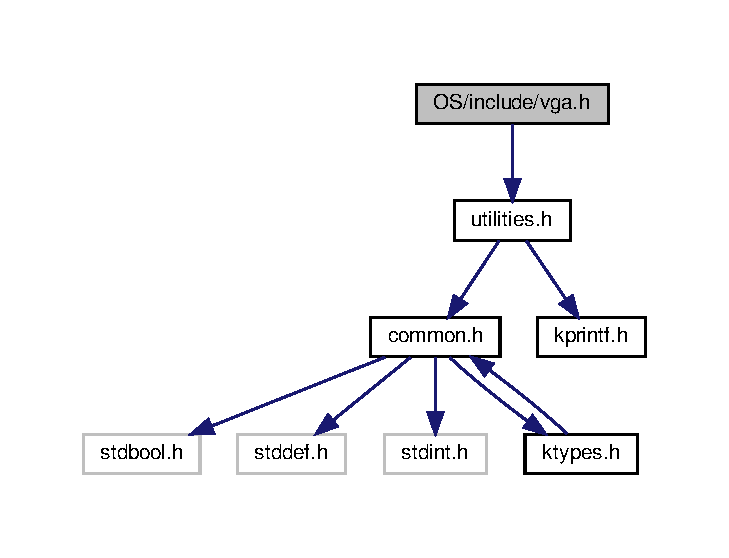
\includegraphics[width=350pt]{vga_8h__incl}
\end{center}
\end{figure}
This graph shows which files directly or indirectly include this file\+:
\nopagebreak
\begin{figure}[H]
\begin{center}
\leavevmode
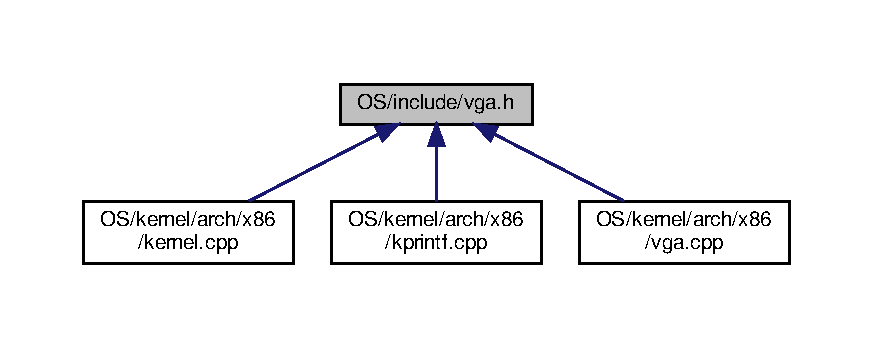
\includegraphics[width=350pt]{vga_8h__dep__incl}
\end{center}
\end{figure}
\subsection*{Classes}
\begin{DoxyCompactItemize}
\item 
class \hyperlink{class_v_g_a_1_1_vga}{V\+G\+A\+::\+Vga}
\end{DoxyCompactItemize}
\subsection*{Namespaces}
\begin{DoxyCompactItemize}
\item 
 \hyperlink{namespace_v_g_a}{V\+GA}
\item 
 \hyperlink{namespace_i_n_i_t}{I\+N\+IT}
\end{DoxyCompactItemize}
\subsection*{Typedefs}
\begin{DoxyCompactItemize}
\item 
typedef uint8\+\_\+t \hyperlink{namespace_v_g_a_afa3882cddefd08a3f33aaf6fcbcbcd7f}{V\+G\+A\+::\+Vga\+Color}
\item 
typedef uint16\+\_\+t \hyperlink{namespace_v_g_a_adb876ce4a116e09f39708ca16ef25f74}{V\+G\+A\+::\+Vga\+Char}
\end{DoxyCompactItemize}
\subsection*{Enumerations}
\begin{DoxyCompactItemize}
\item 
enum \hyperlink{namespace_v_g_a_ace1c3156a8d3975ff783ff7a1fa8eb71}{V\+G\+A\+::\+C\+O\+L\+OR} \+: uint8\+\_\+t \{ \newline
\hyperlink{namespace_v_g_a_ace1c3156a8d3975ff783ff7a1fa8eb71a08d0012388564e95c3b4a7407cf04965}{V\+G\+A\+::\+C\+O\+L\+O\+R\+::\+B\+L\+A\+CK} = 0, 
\hyperlink{namespace_v_g_a_ace1c3156a8d3975ff783ff7a1fa8eb71a1b3e1ee9bff86431dea6b181365ba65f}{V\+G\+A\+::\+C\+O\+L\+O\+R\+::\+B\+L\+UE}, 
\hyperlink{namespace_v_g_a_ace1c3156a8d3975ff783ff7a1fa8eb71a9de0e5dd94e861317e74964bed179fa0}{V\+G\+A\+::\+C\+O\+L\+O\+R\+::\+G\+R\+E\+EN}, 
\hyperlink{namespace_v_g_a_ace1c3156a8d3975ff783ff7a1fa8eb71a344dd8cd533280795b9db82ef0c92749}{V\+G\+A\+::\+C\+O\+L\+O\+R\+::\+C\+Y\+AN}, 
\newline
\hyperlink{namespace_v_g_a_ace1c3156a8d3975ff783ff7a1fa8eb71aa2d9547b5d3dd9f05984475f7c926da0}{V\+G\+A\+::\+C\+O\+L\+O\+R\+::\+R\+ED}, 
\hyperlink{namespace_v_g_a_ace1c3156a8d3975ff783ff7a1fa8eb71ac634ffea7195608364671ac52ee59a61}{V\+G\+A\+::\+C\+O\+L\+O\+R\+::\+M\+A\+G\+E\+N\+TA}, 
\hyperlink{namespace_v_g_a_ace1c3156a8d3975ff783ff7a1fa8eb71a493cacf6f6a2ae4798b319b8b9ba9488}{V\+G\+A\+::\+C\+O\+L\+O\+R\+::\+B\+R\+O\+WN}, 
\hyperlink{namespace_v_g_a_ace1c3156a8d3975ff783ff7a1fa8eb71a0e9d5dda7abbbd2114b24cacd5a6b7af}{V\+G\+A\+::\+C\+O\+L\+O\+R\+::\+L\+I\+G\+H\+T\+\_\+\+G\+R\+EY}, 
\newline
\hyperlink{namespace_v_g_a_ace1c3156a8d3975ff783ff7a1fa8eb71aca9bc0b0de22cd472b6f2716c30dfa94}{V\+G\+A\+::\+C\+O\+L\+O\+R\+::\+D\+A\+R\+K\+\_\+\+G\+R\+EY}, 
\hyperlink{namespace_v_g_a_ace1c3156a8d3975ff783ff7a1fa8eb71a75841220482e3739a9158033b7508cf0}{V\+G\+A\+::\+C\+O\+L\+O\+R\+::\+L\+I\+G\+H\+T\+\_\+\+B\+L\+UE}, 
\hyperlink{namespace_v_g_a_ace1c3156a8d3975ff783ff7a1fa8eb71a555a47662547aa7870851b2ef9ade925}{V\+G\+A\+::\+C\+O\+L\+O\+R\+::\+L\+I\+G\+H\+T\+\_\+\+G\+R\+E\+EN}, 
\hyperlink{namespace_v_g_a_ace1c3156a8d3975ff783ff7a1fa8eb71af3d26561b2c9540ce0714321012a959e}{V\+G\+A\+::\+C\+O\+L\+O\+R\+::\+L\+I\+G\+H\+T\+\_\+\+C\+Y\+AN}, 
\newline
\hyperlink{namespace_v_g_a_ace1c3156a8d3975ff783ff7a1fa8eb71a72722ff9e2a9326d5813c4045d3b4a23}{V\+G\+A\+::\+C\+O\+L\+O\+R\+::\+L\+I\+G\+H\+T\+\_\+\+R\+ED}, 
\hyperlink{namespace_v_g_a_ace1c3156a8d3975ff783ff7a1fa8eb71a0bdcb18cd1ed53fe818fb73e9e9589ef}{V\+G\+A\+::\+C\+O\+L\+O\+R\+::\+L\+I\+G\+H\+T\+\_\+\+M\+A\+G\+E\+N\+TA}, 
\hyperlink{namespace_v_g_a_ace1c3156a8d3975ff783ff7a1fa8eb71a91787c73bd6b00fe2723ed0194921dc4}{V\+G\+A\+::\+C\+O\+L\+O\+R\+::\+L\+I\+G\+H\+T\+\_\+\+B\+R\+O\+WN}, 
\hyperlink{namespace_v_g_a_ace1c3156a8d3975ff783ff7a1fa8eb71ab5bf627e448384cf3a4c35121ca6008d}{V\+G\+A\+::\+C\+O\+L\+O\+R\+::\+W\+H\+I\+TE}
 \}
\end{DoxyCompactItemize}
\subsection*{Functions}
\begin{DoxyCompactItemize}
\item 
void \hyperlink{namespace_i_n_i_t_abae5789d80f8edd37455f3b167779654}{I\+N\+I\+T\+::\+V\+GA} ()
\end{DoxyCompactItemize}

\hypertarget{virtualmemory_8h}{}\section{O\+S/include/virtualmemory.h File Reference}
\label{virtualmemory_8h}\index{O\+S/include/virtualmemory.\+h@{O\+S/include/virtualmemory.\+h}}
{\ttfamily \#include $<$common.\+h$>$}\newline
{\ttfamily \#include $<$utilities.\+h$>$}\newline
Include dependency graph for virtualmemory.\+h\+:\nopagebreak
\begin{figure}[H]
\begin{center}
\leavevmode
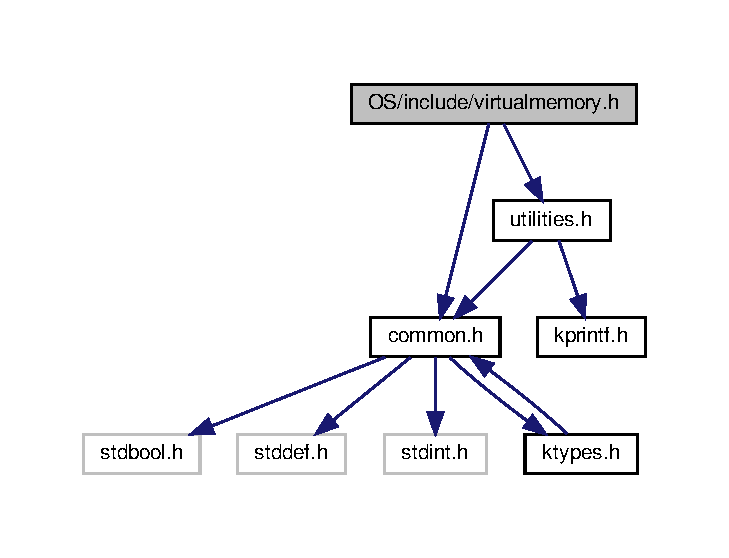
\includegraphics[width=350pt]{virtualmemory_8h__incl}
\end{center}
\end{figure}
This graph shows which files directly or indirectly include this file\+:\nopagebreak
\begin{figure}[H]
\begin{center}
\leavevmode
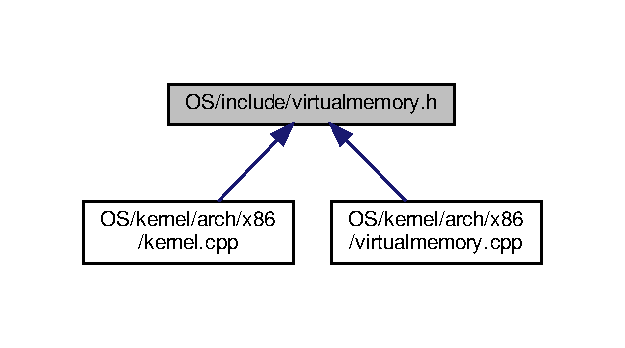
\includegraphics[width=300pt]{virtualmemory_8h__dep__incl}
\end{center}
\end{figure}
\subsection*{Namespaces}
\begin{DoxyCompactItemize}
\item 
 \hyperlink{namespace_i_n_i_t}{I\+N\+IT}
\begin{DoxyCompactList}\small\item\em contains all kernel initialization routines \end{DoxyCompactList}\item 
 \hyperlink{namespace_v_m}{VM}
\begin{DoxyCompactList}\small\item\em Virtual memory namespace. \end{DoxyCompactList}\item 
 \hyperlink{namespace_v_m_1_1_p_d_a}{V\+M\+::\+P\+DA}
\begin{DoxyCompactList}\small\item\em Page directory access (lower 12 bits of page directory entry) \end{DoxyCompactList}\item 
 \hyperlink{namespace_v_m_1_1_p_t_a}{V\+M\+::\+P\+TA}
\begin{DoxyCompactList}\small\item\em Page table access (lower 12 bits of page table entry) \end{DoxyCompactList}\end{DoxyCompactItemize}
\subsection*{Enumerations}
\begin{DoxyCompactItemize}
\item 
enum \+: uint16\+\_\+t \{ \newline
\hyperlink{namespace_v_m_1_1_p_d_a_a7a5d6d32b47f20a14422314b14fdc591a2f8ff50210f87689944543ed655971cb}{V\+M\+::\+P\+D\+A\+::P} = 0, 
\hyperlink{namespace_v_m_1_1_p_d_a_a7a5d6d32b47f20a14422314b14fdc591a80249bc62c8a67e157d2b13cdf4325f7}{V\+M\+::\+P\+D\+A\+::R} = 1, 
\hyperlink{namespace_v_m_1_1_p_d_a_a7a5d6d32b47f20a14422314b14fdc591ad295b7d3bddcf79dc55d6e5c90423c2b}{V\+M\+::\+P\+D\+A\+::U} = 2, 
\hyperlink{namespace_v_m_1_1_p_d_a_a7a5d6d32b47f20a14422314b14fdc591a8a740302ea12c8d4c4d5a47ac1af683f}{V\+M\+::\+P\+D\+A\+::W} = 3, 
\newline
\hyperlink{namespace_v_m_1_1_p_d_a_a7a5d6d32b47f20a14422314b14fdc591a6243d3f10651bfe05301f7cdfafaa6aa}{V\+M\+::\+P\+D\+A\+::D} = 4, 
\hyperlink{namespace_v_m_1_1_p_d_a_a7a5d6d32b47f20a14422314b14fdc591a55148405937cb89c60ff92caaadf8dfa}{V\+M\+::\+P\+D\+A\+::A} = 5, 
\hyperlink{namespace_v_m_1_1_p_d_a_a7a5d6d32b47f20a14422314b14fdc591a46023444e176bb33206552f231471c37}{V\+M\+::\+P\+D\+A\+::S} = 7
 \}
\item 
enum \+: uint16\+\_\+t \{ \newline
\hyperlink{namespace_v_m_1_1_p_t_a_a89a9cf444829a1e2681beab7a219fea5a807772f9595a363566fba6fdf733e8f9}{V\+M\+::\+P\+T\+A\+::P} = 0, 
\hyperlink{namespace_v_m_1_1_p_t_a_a89a9cf444829a1e2681beab7a219fea5a8845432dbb156062ae5103d618c41d75}{V\+M\+::\+P\+T\+A\+::R} = 1, 
\hyperlink{namespace_v_m_1_1_p_t_a_a89a9cf444829a1e2681beab7a219fea5a1328ecb0d0d696708fff0e2492b864be}{V\+M\+::\+P\+T\+A\+::U} = 2, 
\hyperlink{namespace_v_m_1_1_p_t_a_a89a9cf444829a1e2681beab7a219fea5a09b0f0ebacacbb343e02d17dedc2ed4e}{V\+M\+::\+P\+T\+A\+::W} = 3, 
\newline
\hyperlink{namespace_v_m_1_1_p_t_a_a89a9cf444829a1e2681beab7a219fea5a789da119278c61f741fe1ed3efc8e0d3}{V\+M\+::\+P\+T\+A\+::C} = 4, 
\hyperlink{namespace_v_m_1_1_p_t_a_a89a9cf444829a1e2681beab7a219fea5a0bffb3e999362e382526209e130dec62}{V\+M\+::\+P\+T\+A\+::A} = 5, 
\hyperlink{namespace_v_m_1_1_p_t_a_a89a9cf444829a1e2681beab7a219fea5ac77057cf7fa6ca270c2b31f0c24125df}{V\+M\+::\+P\+T\+A\+::D} = 6, 
\hyperlink{namespace_v_m_1_1_p_t_a_a89a9cf444829a1e2681beab7a219fea5a07e37da4a960b9f69565a92c812da75c}{V\+M\+::\+P\+T\+A\+::G} = 8
 \}
\end{DoxyCompactItemize}
\subsection*{Functions}
\begin{DoxyCompactItemize}
\item 
void \hyperlink{namespace_i_n_i_t_aea383d3de30095cf9d176fa60b66d01d}{I\+N\+I\+T\+::\+P\+A\+GE} ()
\begin{DoxyCompactList}\small\item\em set up page directory, page table, and turn on paging \end{DoxyCompactList}\end{DoxyCompactItemize}

\hypertarget{cpu_8cpp}{}\section{O\+S/kernel/arch/x86/cpu.cpp File Reference}
\label{cpu_8cpp}\index{O\+S/kernel/arch/x86/cpu.\+cpp@{O\+S/kernel/arch/x86/cpu.\+cpp}}
{\ttfamily \#include $<$common.\+h$>$}\newline
{\ttfamily \#include $<$utilities.\+h$>$}\newline
{\ttfamily \#include $<$kprintf.\+h$>$}\newline
{\ttfamily \#include $<$registers.\+h$>$}\newline
Include dependency graph for cpu.\+cpp\+:
\nopagebreak
\begin{figure}[H]
\begin{center}
\leavevmode
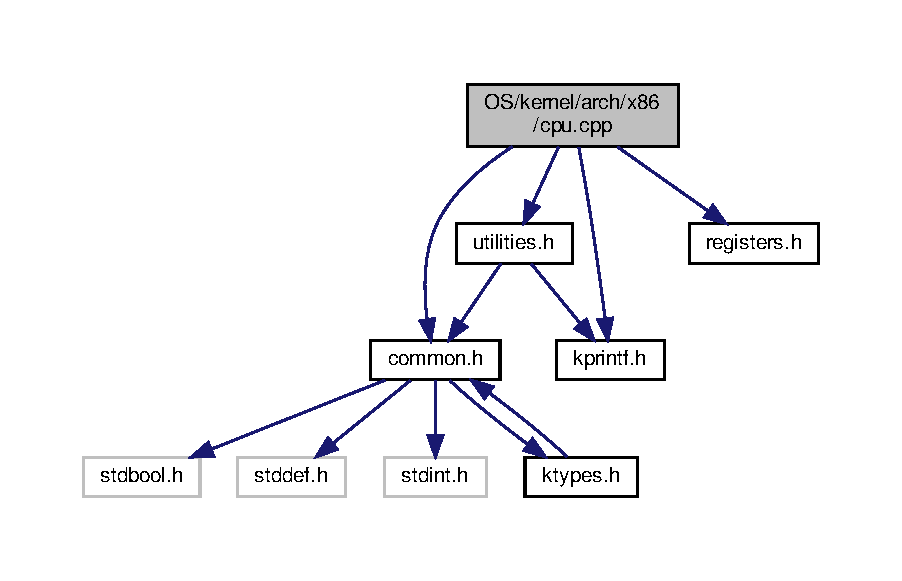
\includegraphics[width=350pt]{cpu_8cpp__incl}
\end{center}
\end{figure}
\subsection*{Namespaces}
\begin{DoxyCompactItemize}
\item 
 \hyperlink{namespace_i_n_i_t}{I\+N\+IT}
\end{DoxyCompactItemize}
\subsection*{Functions}
\begin{DoxyCompactItemize}
\item 
void \hyperlink{namespace_i_n_i_t_a8928ddbb4ca671dfe1c740da380fa0c4}{I\+N\+I\+T\+::\+S\+SE} ()
\end{DoxyCompactItemize}

\hypertarget{gdt_8cpp}{}\section{O\+S/kernel/arch/x86/gdt.cpp File Reference}
\label{gdt_8cpp}\index{O\+S/kernel/arch/x86/gdt.\+cpp@{O\+S/kernel/arch/x86/gdt.\+cpp}}
{\ttfamily \#include $<$common.\+h$>$}\newline
{\ttfamily \#include $<$gdt.\+h$>$}\newline
{\ttfamily \#include $<$utilities.\+h$>$}\newline
{\ttfamily \#include $<$registers.\+h$>$}\newline
{\ttfamily \#include $<$accessright.\+h$>$}\newline
Include dependency graph for gdt.\+cpp\+:
\nopagebreak
\begin{figure}[H]
\begin{center}
\leavevmode
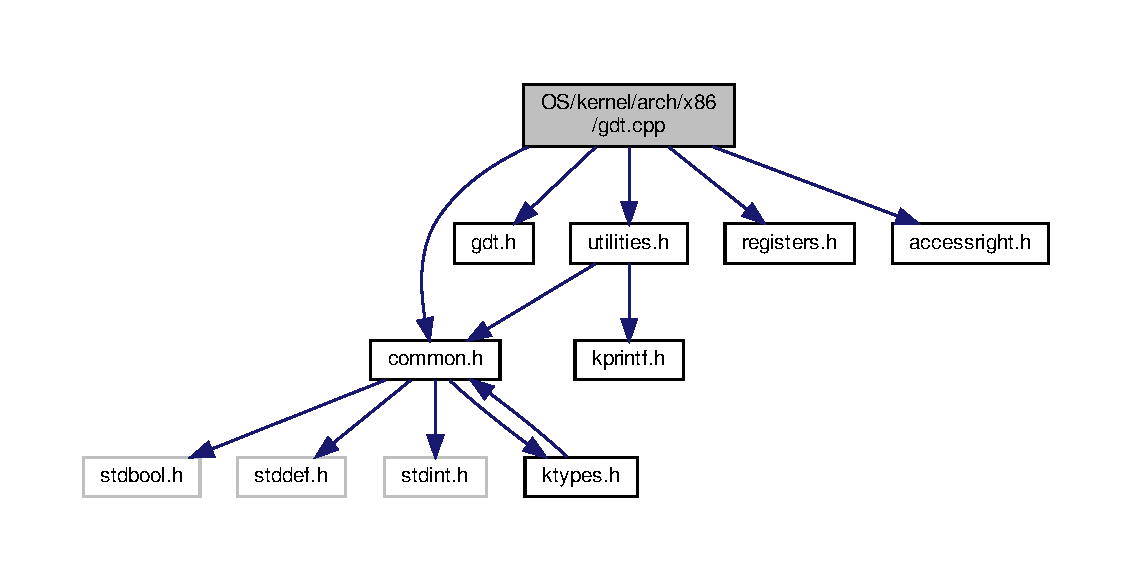
\includegraphics[width=350pt]{gdt_8cpp__incl}
\end{center}
\end{figure}
\subsection*{Classes}
\begin{DoxyCompactItemize}
\item 
struct \hyperlink{struct_g_d_t_1_1_selector}{G\+D\+T\+::\+Selector}
\end{DoxyCompactItemize}
\subsection*{Namespaces}
\begin{DoxyCompactItemize}
\item 
 \hyperlink{namespace_g_d_t}{G\+DT}
\item 
 \hyperlink{namespace_i_n_i_t}{I\+N\+IT}
\end{DoxyCompactItemize}
\subsection*{Functions}
\begin{DoxyCompactItemize}
\item 
union \hyperlink{namespace_g_d_t_aafeef73468f65116a440104dd6359e4c}{G\+D\+T\+::\+\_\+\+\_\+attribute\+\_\+\+\_\+} ((packed)) Gdt\+Entry
\item 
void \hyperlink{namespace_g_d_t_a5d0041eb890e6c1f40d8a919494c2354}{G\+D\+T\+::\+Set\+Global\+Descriptor\+Entry} (Gdt\+Entry Gdt\+Table\mbox{[}$\,$\mbox{]}, const Selector Selector\+Table\mbox{[}$\,$\mbox{]})
\item 
void \hyperlink{namespace_g_d_t_a3660563d28e3bab08ddac58ca6844b58}{G\+D\+T\+::\+Load\+\_\+gdt} (void $\ast$gdt\+Address, uint16\+\_\+t Limit\+Use)
\item 
void \hyperlink{namespace_g_d_t_a174feb7c5a037cc991bf4eb27c256366}{G\+D\+T\+::\+Install\+\_\+gdt} ()
\item 
void \hyperlink{namespace_i_n_i_t_a3462d7bc51bce77cc240d05b62b1b777}{I\+N\+I\+T\+::gdt} ()
\end{DoxyCompactItemize}
\subsection*{Variables}
\begin{DoxyCompactItemize}
\item 
const uint32\+\_\+t \hyperlink{namespace_g_d_t_aa1bc8e5b9e4868b6006698829d396724}{G\+D\+T\+::\+N\+U\+L\+L\+\_\+\+L\+I\+M\+IT} = 0x00000000
\item 
const uint32\+\_\+t \hyperlink{namespace_g_d_t_ab6d06fd71d054410909a4aacafca32b7}{G\+D\+T\+::\+K\+E\+R\+N\+\_\+\+C\+S\+\_\+\+L\+I\+M\+IT} = 0x000\+F\+F\+F\+FF
\item 
const uint32\+\_\+t \hyperlink{namespace_g_d_t_a0b19f62da26fef63c425face3191a75b}{G\+D\+T\+::\+K\+E\+R\+N\+\_\+\+D\+S\+\_\+\+L\+I\+M\+IT} = 0x000\+F\+F\+F\+FF
\item 
const uint32\+\_\+t \hyperlink{namespace_g_d_t_af9547432d12ed931a8aafe2f078bfdb9}{G\+D\+T\+::\+U\+S\+E\+R\+\_\+\+C\+S\+\_\+\+L\+I\+M\+IT} = 0x000\+F\+F\+F\+FF
\item 
const uint32\+\_\+t \hyperlink{namespace_g_d_t_a65f624eed850cd303b27f014e43576e4}{G\+D\+T\+::\+U\+S\+E\+R\+\_\+\+D\+S\+\_\+\+L\+I\+M\+IT} = 0x000\+F\+F\+F\+FF
\item 
const uint32\+\_\+t \hyperlink{namespace_g_d_t_a99c336ac1e41e7292c0da263389748d7}{G\+D\+T\+::\+N\+U\+L\+L\+\_\+\+B\+A\+SE} = 0x00000000
\item 
const uint32\+\_\+t \hyperlink{namespace_g_d_t_aa468dabc4b15ceac65292f59b3d98e76}{G\+D\+T\+::\+K\+E\+R\+N\+\_\+\+C\+S\+\_\+\+B\+A\+SE} = 0x00000000
\item 
const uint32\+\_\+t \hyperlink{namespace_g_d_t_a2a50b369a9ea36da4724c269a2c005a2}{G\+D\+T\+::\+K\+E\+R\+N\+\_\+\+D\+S\+\_\+\+B\+A\+SE} = 0x00000000
\item 
const uint32\+\_\+t \hyperlink{namespace_g_d_t_a17592b6bcda3da0b4162793c5ab25d34}{G\+D\+T\+::\+U\+S\+E\+R\+\_\+\+C\+S\+\_\+\+B\+A\+SE} = 0x00000000
\item 
const uint32\+\_\+t \hyperlink{namespace_g_d_t_af3b358f3263317a93fb70214db0fe9df}{G\+D\+T\+::\+U\+S\+E\+R\+\_\+\+D\+S\+\_\+\+B\+A\+SE} = 0x00000000
\item 
const uint8\+\_\+t \hyperlink{namespace_g_d_t_ac7317e2289378a4e654f8137e837e954}{G\+D\+T\+::\+N\+U\+L\+L\+\_\+\+G\+R\+A\+N\+U\+L\+A\+R\+I\+TY} = 0x00
\item 
const uint8\+\_\+t \hyperlink{namespace_g_d_t_a1ff5f5e1d41e01c0c4c32711264a5e23}{G\+D\+T\+::\+K\+E\+R\+N\+\_\+\+C\+S\+\_\+\+G\+R\+A\+N\+U\+L\+A\+R\+I\+TY} = 0x\+C0
\item 
const uint8\+\_\+t \hyperlink{namespace_g_d_t_a93b62ba7a382d7801e63bd32655a87c3}{G\+D\+T\+::\+K\+E\+R\+N\+\_\+\+D\+S\+\_\+\+G\+R\+A\+N\+U\+L\+A\+R\+I\+TY} = 0x\+C0
\item 
const uint8\+\_\+t \hyperlink{namespace_g_d_t_abca29cbf8c95b79a247c1b7af347deba}{G\+D\+T\+::\+U\+S\+E\+R\+\_\+\+C\+S\+\_\+\+G\+R\+A\+N\+U\+L\+A\+R\+I\+TY} = 0x\+C0
\item 
const uint8\+\_\+t \hyperlink{namespace_g_d_t_a1d41acb5aa3d1b3690fb1fa6e843f110}{G\+D\+T\+::\+U\+S\+E\+R\+\_\+\+D\+S\+\_\+\+G\+R\+A\+N\+U\+L\+A\+R\+I\+TY} = 0x\+C0
\end{DoxyCompactItemize}

\hypertarget{global_8cpp}{}\section{O\+S/kernel/arch/x86/global.cpp File Reference}
\label{global_8cpp}\index{O\+S/kernel/arch/x86/global.\+cpp@{O\+S/kernel/arch/x86/global.\+cpp}}
{\ttfamily \#include $<$global.\+h$>$}\newline
{\ttfamily \#include $<$ktypes.\+h$>$}\newline
Include dependency graph for global.\+cpp\+:\nopagebreak
\begin{figure}[H]
\begin{center}
\leavevmode
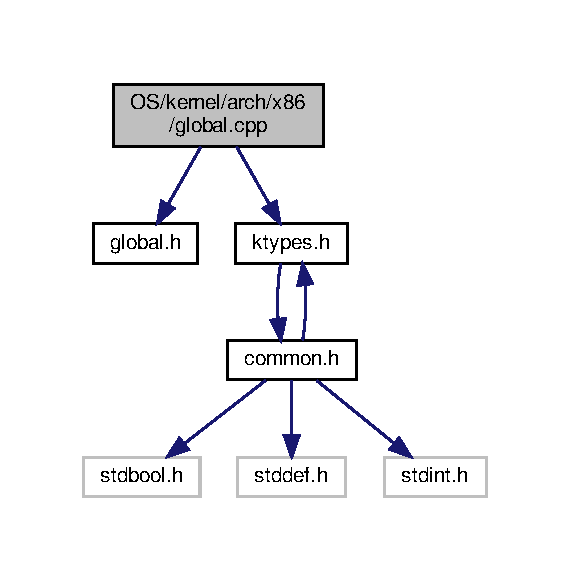
\includegraphics[width=274pt]{global_8cpp__incl}
\end{center}
\end{figure}
\subsection*{Namespaces}
\begin{DoxyCompactItemize}
\item 
 \hyperlink{namespace_i_n_i_t}{I\+N\+IT}
\begin{DoxyCompactList}\small\item\em contains all kernel initialization routines \end{DoxyCompactList}\end{DoxyCompactItemize}
\subsection*{Functions}
\begin{DoxyCompactItemize}
\item 
void \hyperlink{namespace_i_n_i_t_a6608557e41ad37cdb4a408e2f05c9783}{I\+N\+I\+T\+::ctors} ()
\begin{DoxyCompactList}\small\item\em calls constructors on all global objects \end{DoxyCompactList}\end{DoxyCompactItemize}
\subsection*{Variables}
\begin{DoxyCompactItemize}
\item 
\hyperlink{ktypes_8h_a46bbb9e776183ed6a8eca9d919756434}{func\+\_\+ptr} \hyperlink{global_8cpp_a00261bc929e9f609199f22bc18ff9d95}{start\+\_\+ctors}
\begin{DoxyCompactList}\small\item\em starting address of pointers to global constructors \end{DoxyCompactList}\item 
\hyperlink{ktypes_8h_a46bbb9e776183ed6a8eca9d919756434}{func\+\_\+ptr} \hyperlink{global_8cpp_a81e8429b21b9b2903ec5fa67d3328eae}{end\+\_\+ctors}
\begin{DoxyCompactList}\small\item\em ending address of pointers to global constructors \end{DoxyCompactList}\end{DoxyCompactItemize}


\subsection{Variable Documentation}
\mbox{\Hypertarget{global_8cpp_a81e8429b21b9b2903ec5fa67d3328eae}\label{global_8cpp_a81e8429b21b9b2903ec5fa67d3328eae}} 
\index{global.\+cpp@{global.\+cpp}!end\+\_\+ctors@{end\+\_\+ctors}}
\index{end\+\_\+ctors@{end\+\_\+ctors}!global.\+cpp@{global.\+cpp}}
\subsubsection{\texorpdfstring{end\+\_\+ctors}{end\_ctors}}
{\footnotesize\ttfamily \hyperlink{ktypes_8h_a46bbb9e776183ed6a8eca9d919756434}{func\+\_\+ptr} end\+\_\+ctors}



ending address of pointers to global constructors 

symbol defined in \hyperlink{linker_8ld}{linker.\+ld}. \mbox{\Hypertarget{global_8cpp_a00261bc929e9f609199f22bc18ff9d95}\label{global_8cpp_a00261bc929e9f609199f22bc18ff9d95}} 
\index{global.\+cpp@{global.\+cpp}!start\+\_\+ctors@{start\+\_\+ctors}}
\index{start\+\_\+ctors@{start\+\_\+ctors}!global.\+cpp@{global.\+cpp}}
\subsubsection{\texorpdfstring{start\+\_\+ctors}{start\_ctors}}
{\footnotesize\ttfamily \hyperlink{ktypes_8h_a46bbb9e776183ed6a8eca9d919756434}{func\+\_\+ptr} start\+\_\+ctors}



starting address of pointers to global constructors 

symbol defined in \hyperlink{linker_8ld}{linker.\+ld}. 
\hypertarget{interrupt_8cpp}{}\section{O\+S/kernel/arch/x86/interrupt.cpp File Reference}
\label{interrupt_8cpp}\index{O\+S/kernel/arch/x86/interrupt.\+cpp@{O\+S/kernel/arch/x86/interrupt.\+cpp}}
{\ttfamily \#include $<$common.\+h$>$}\newline
{\ttfamily \#include $<$interrupt.\+h$>$}\newline
{\ttfamily \#include $<$utilities.\+h$>$}\newline
{\ttfamily \#include $<$gdt.\+h$>$}\newline
{\ttfamily \#include $<$accessright.\+h$>$}\newline
Include dependency graph for interrupt.\+cpp\+:\nopagebreak
\begin{figure}[H]
\begin{center}
\leavevmode
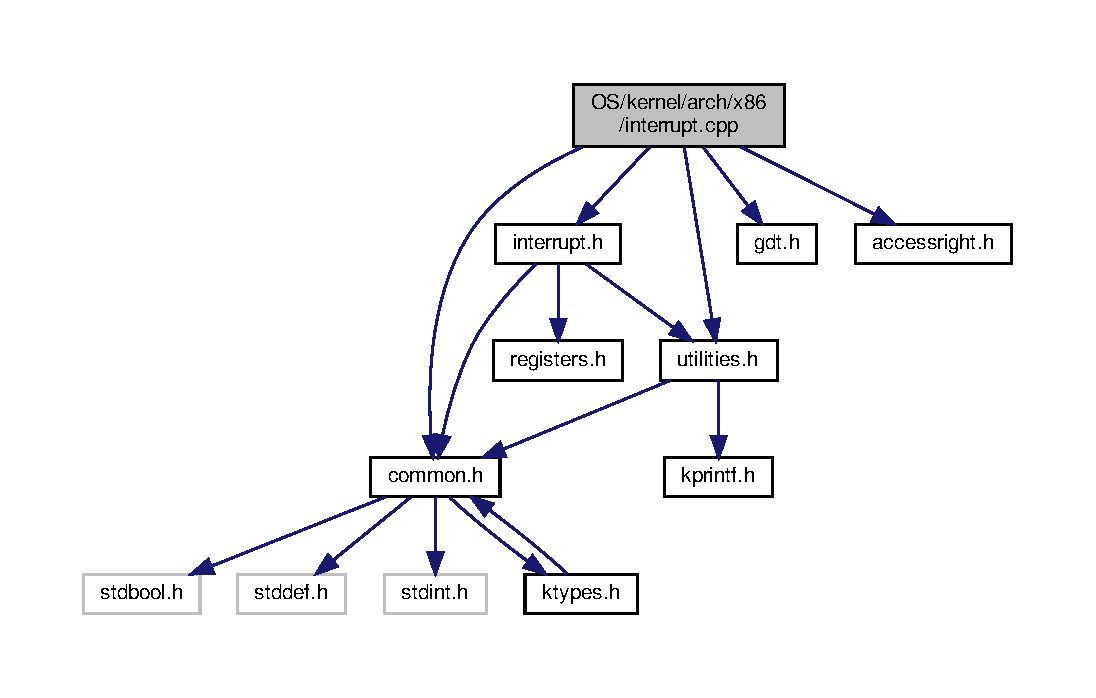
\includegraphics[width=350pt]{interrupt_8cpp__incl}
\end{center}
\end{figure}
\subsection*{Namespaces}
\begin{DoxyCompactItemize}
\item 
 \hyperlink{namespace_p_i_c}{P\+IC}
\begin{DoxyCompactList}\small\item\em 8259 Progammable interrupt controller \end{DoxyCompactList}\item 
 \hyperlink{namespace_i_n_t_r_p}{I\+N\+T\+RP}
\begin{DoxyCompactList}\small\item\em interrupt namespace \end{DoxyCompactList}\item 
 \hyperlink{namespace_i_n_i_t}{I\+N\+IT}
\begin{DoxyCompactList}\small\item\em contains all kernel initialization routines \end{DoxyCompactList}\end{DoxyCompactItemize}
\subsection*{Functions}
\begin{DoxyCompactItemize}
\item 
void \hyperlink{namespace_p_i_c_a2a04fe95329faacc43f00ad30fe554b9}{P\+I\+C\+::\+Remap} ()
\begin{DoxyCompactList}\small\item\em Remap default 8259 \hyperlink{namespace_p_i_c}{P\+IC} interrupt number to new range. \end{DoxyCompactList}\item 
void \hyperlink{namespace_p_i_c_ad6f2cca6611cd7992992ab7705d6c25f}{P\+I\+C\+::\+Unmask\+Interrupt} (uint16\+\_\+t Port, uint8\+\_\+t Irq)
\item 
void \hyperlink{namespace_i_n_t_r_p_a91a6a2668bfa9961a9ed265f6ceac47d}{I\+N\+T\+R\+P\+::\+Register\+Handler} (Descriptor\+Entry Idt\+Table\mbox{[}$\,$\mbox{]}, size\+\_\+t Idx, \hyperlink{ktypes_8h_a46bbb9e776183ed6a8eca9d919756434}{func\+\_\+ptr} Handler)
\begin{DoxyCompactList}\small\item\em Creates interrupt descriptor entries in idt\+\_\+table, and loads into C\+PU. \end{DoxyCompactList}\item 
void \hyperlink{namespace_i_n_t_r_p_a7732859732913734b09dd07030c41991}{I\+N\+T\+R\+P\+::\+Unhandled\+Exception} ()
\begin{DoxyCompactList}\small\item\em default unhandled exception handler \end{DoxyCompactList}\item 
void \hyperlink{namespace_i_n_t_r_p_a0232249076503af19eee46e59a4e5bb8}{I\+N\+T\+R\+P\+::\+Timer\+Interrupt\+Handler} ()
\begin{DoxyCompactList}\small\item\em Timer interrupt handler. \end{DoxyCompactList}\item 
void \hyperlink{namespace_i_n_t_r_p_aff35666b88439353d86e253d3051f27f}{I\+N\+T\+R\+P\+::\+Page\+Fault\+Handler} ()
\begin{DoxyCompactList}\small\item\em Page fault handler. \end{DoxyCompactList}\item 
void \hyperlink{namespace_i_n_t_r_p_a13c03019c9d7b305743516310096a82a}{I\+N\+T\+R\+P\+::\+Unhandled\+Interrupt} ()
\begin{DoxyCompactList}\small\item\em default unhandled interrupt handler \end{DoxyCompactList}\item 
void \hyperlink{namespace_i_n_t_r_p_a4a1a1ff73a4e9bb1c17daf205170daa9}{I\+N\+T\+R\+P\+::\+Set\+Exception\+Handler} (Descriptor\+Entry Idt\+Table\mbox{[}$\,$\mbox{]})
\begin{DoxyCompactList}\small\item\em Installs default exception handler to all exceptions. \end{DoxyCompactList}\item 
void \hyperlink{namespace_i_n_t_r_p_abf09ee877603981fe255cd050cbbb110}{I\+N\+T\+R\+P\+::\+Set\+Interrupt\+Handler} (Descriptor\+Entry Idt\+Table\mbox{[}$\,$\mbox{]})
\begin{DoxyCompactList}\small\item\em Installs default interrupt handler to all interrupts. \end{DoxyCompactList}\item 
void \hyperlink{namespace_i_n_t_r_p_a194f85d6c873615e9125466e3b23c30f}{I\+N\+T\+R\+P\+::\+Load\+\_\+lidt} (void $\ast$lidt\+Address, uint16\+\_\+t Limit\+Use)
\begin{DoxyCompactList}\small\item\em assembly instruction to load idt table to C\+PU \end{DoxyCompactList}\item 
void \hyperlink{namespace_i_n_t_r_p_a139b273cc1e45d3c2fdfe0d387a98518}{I\+N\+T\+R\+P\+::\+Install\+\_\+idt} ()
\begin{DoxyCompactList}\small\item\em Assigns exception and interrupt handler to idt\+\_\+table, and load to C\+PU. \end{DoxyCompactList}\item 
void \hyperlink{namespace_i_n_i_t_aec8e9f01cb09653075b6e610096b3ca9}{I\+N\+I\+T\+::idt} ()
\begin{DoxyCompactList}\small\item\em Creates interrupt descriptor table and loads to C\+PU. \end{DoxyCompactList}\end{DoxyCompactItemize}
\subsection*{Variables}
\begin{DoxyCompactItemize}
\item 
Descriptor\+Entry \hyperlink{namespace_i_n_t_r_p_a8e4e29dae90a4087ed1ac8cf845218c4}{I\+N\+T\+R\+P\+::idt\+\_\+table} \mbox{[}I\+D\+T\+\_\+\+E\+N\+T\+R\+I\+ES\mbox{]}
\end{DoxyCompactItemize}

\hypertarget{kernel_8cpp}{}\section{O\+S/kernel/arch/x86/kernel.cpp File Reference}
\label{kernel_8cpp}\index{O\+S/kernel/arch/x86/kernel.\+cpp@{O\+S/kernel/arch/x86/kernel.\+cpp}}
{\ttfamily \#include $<$common.\+h$>$}\newline
{\ttfamily \#include $<$vga.\+h$>$}\newline
{\ttfamily \#include $<$cpu.\+h$>$}\newline
{\ttfamily \#include $<$interrupt.\+h$>$}\newline
{\ttfamily \#include $<$gdt.\+h$>$}\newline
{\ttfamily \#include $<$global.\+h$>$}\newline
{\ttfamily \#include $<$memoryallocator.\+h$>$}\newline
{\ttfamily \#include $<$virtualmemory.\+h$>$}\newline
Include dependency graph for kernel.\+cpp\+:\nopagebreak
\begin{figure}[H]
\begin{center}
\leavevmode
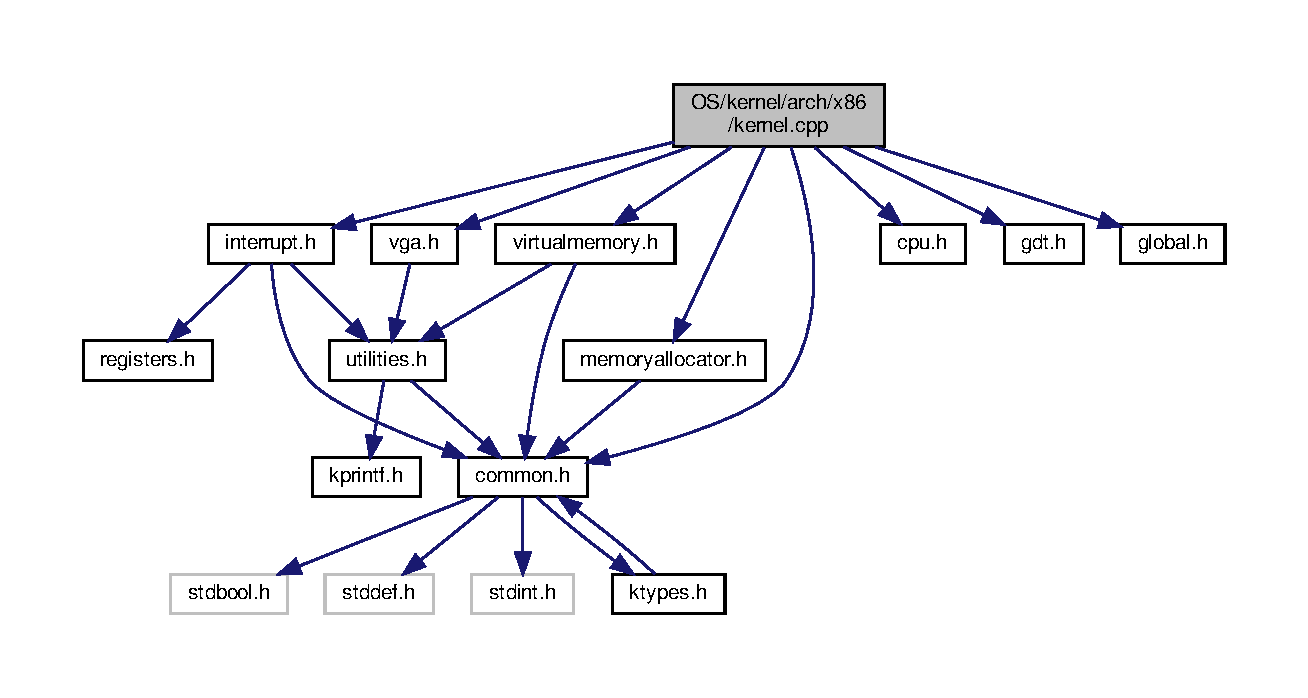
\includegraphics[width=350pt]{kernel_8cpp__incl}
\end{center}
\end{figure}
\subsection*{Functions}
\begin{DoxyCompactItemize}
\item 
void \hyperlink{kernel_8cpp_ada8402e0c504af8cafef5cc76c076003}{kernel\+\_\+main} ()
\begin{DoxyCompactList}\small\item\em Kernel entry function. \end{DoxyCompactList}\end{DoxyCompactItemize}


\subsection{Function Documentation}
\mbox{\Hypertarget{kernel_8cpp_ada8402e0c504af8cafef5cc76c076003}\label{kernel_8cpp_ada8402e0c504af8cafef5cc76c076003}} 
\index{kernel.\+cpp@{kernel.\+cpp}!kernel\+\_\+main@{kernel\+\_\+main}}
\index{kernel\+\_\+main@{kernel\+\_\+main}!kernel.\+cpp@{kernel.\+cpp}}
\subsubsection{\texorpdfstring{kernel\+\_\+main()}{kernel\_main()}}
{\footnotesize\ttfamily void kernel\+\_\+main (\begin{DoxyParamCaption}{ }\end{DoxyParamCaption})}



Kernel entry function. 

\mbox{[}Kernel entry function\mbox{]} 

Definition at line 21 of file kernel.\+cpp.


\hypertarget{kprintf_8cpp}{}\section{O\+S/kernel/arch/x86/kprintf.cpp File Reference}
\label{kprintf_8cpp}\index{O\+S/kernel/arch/x86/kprintf.\+cpp@{O\+S/kernel/arch/x86/kprintf.\+cpp}}
{\ttfamily \#include $<$kprintf.\+h$>$}\newline
{\ttfamily \#include $<$vga.\+h$>$}\newline
Include dependency graph for kprintf.\+cpp\+:
\nopagebreak
\begin{figure}[H]
\begin{center}
\leavevmode
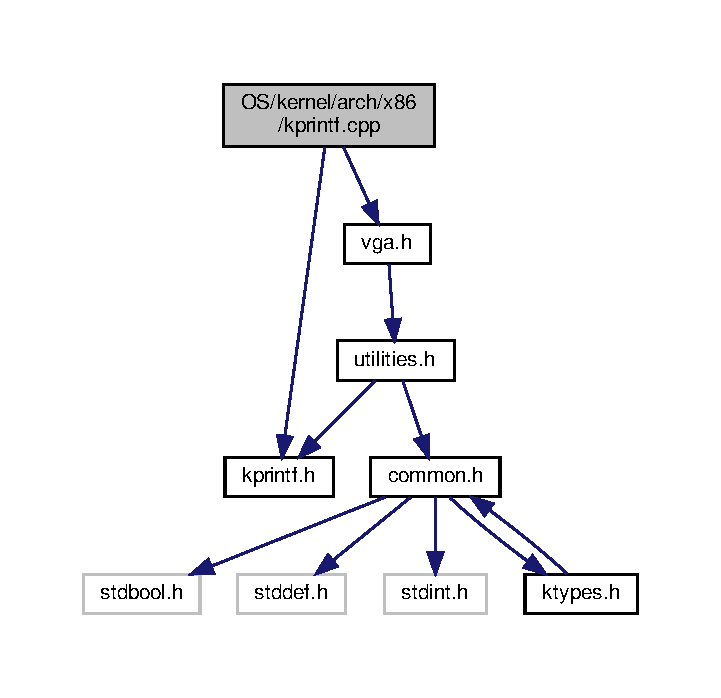
\includegraphics[width=346pt]{kprintf_8cpp__incl}
\end{center}
\end{figure}
\subsection*{Namespaces}
\begin{DoxyCompactItemize}
\item 
 \hyperlink{namespace_v_g_a}{V\+GA}
\end{DoxyCompactItemize}
\subsection*{Functions}
\begin{DoxyCompactItemize}
\item 
void \hyperlink{kprintf_8cpp_ae610f6b2bc90ea3eed7852d591c48116}{kprintf} (const char $\ast$Str)
\end{DoxyCompactItemize}
\subsection*{Variables}
\begin{DoxyCompactItemize}
\item 
Vga \hyperlink{namespace_v_g_a_a97690b6d72f447f3e5e1b744af8f47fe}{V\+G\+A\+::\+Display}
\end{DoxyCompactItemize}


\subsection{Function Documentation}
\mbox{\Hypertarget{kprintf_8cpp_ae610f6b2bc90ea3eed7852d591c48116}\label{kprintf_8cpp_ae610f6b2bc90ea3eed7852d591c48116}} 
\index{kprintf.\+cpp@{kprintf.\+cpp}!kprintf@{kprintf}}
\index{kprintf@{kprintf}!kprintf.\+cpp@{kprintf.\+cpp}}
\subsubsection{\texorpdfstring{kprintf()}{kprintf()}}
{\footnotesize\ttfamily void kprintf (\begin{DoxyParamCaption}\item[{const char $\ast$}]{Str }\end{DoxyParamCaption})}



Definition at line 13 of file kprintf.\+cpp.


\hypertarget{memoryallocator_8cpp}{}\section{O\+S/kernel/arch/x86/memoryallocator.cpp File Reference}
\label{memoryallocator_8cpp}\index{O\+S/kernel/arch/x86/memoryallocator.\+cpp@{O\+S/kernel/arch/x86/memoryallocator.\+cpp}}
{\ttfamily \#include $<$memoryallocator.\+h$>$}\newline
{\ttfamily \#include $<$interrupt.\+h$>$}\newline
{\ttfamily \#include $<$ktypes.\+h$>$}\newline
Include dependency graph for memoryallocator.\+cpp\+:
\nopagebreak
\begin{figure}[H]
\begin{center}
\leavevmode
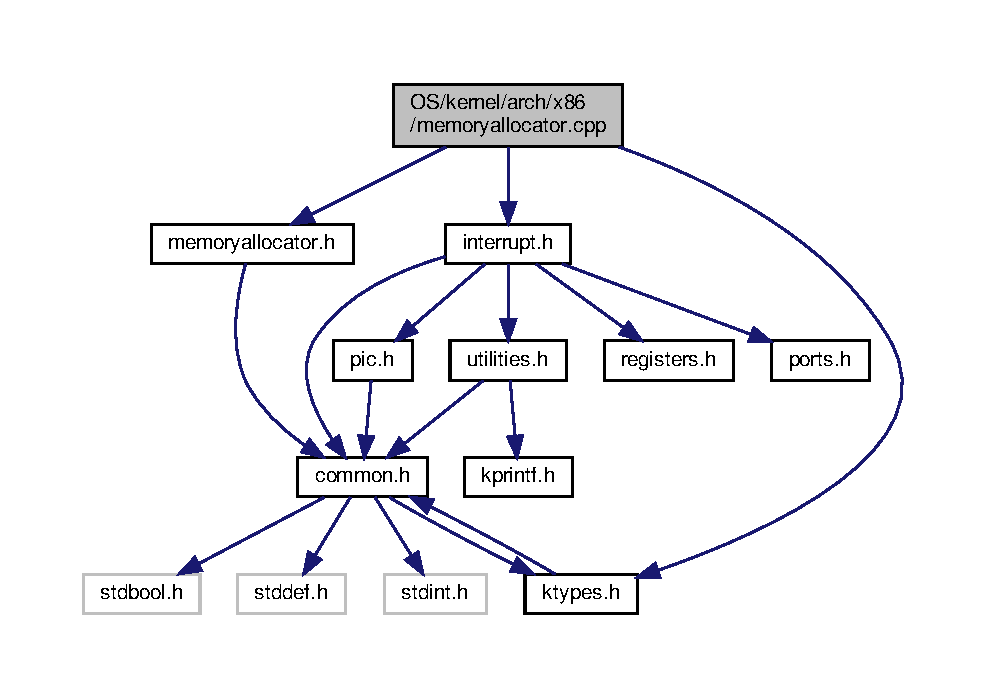
\includegraphics[width=350pt]{memoryallocator_8cpp__incl}
\end{center}
\end{figure}
\subsection*{Namespaces}
\begin{DoxyCompactItemize}
\item 
 \hyperlink{namespace_k_m}{KM}
\begin{DoxyCompactList}\small\item\em Kernel memory namespace. \end{DoxyCompactList}\item 
 \hyperlink{namespace_i_n_i_t}{I\+N\+IT}
\begin{DoxyCompactList}\small\item\em contains all kernel initialization routines \end{DoxyCompactList}\end{DoxyCompactItemize}
\subsection*{Functions}
\begin{DoxyCompactItemize}
\item 
void $\ast$ \hyperlink{namespace_k_m_aaeb8403b430af6311bb3c1df6ae520b6}{K\+M\+::kmalloc} (size\+\_\+t Size)
\begin{DoxyCompactList}\small\item\em kernel malloc \end{DoxyCompactList}\item 
void \hyperlink{namespace_k_m_a08363437a217255f3f9d2a393a54714b}{K\+M\+::free} (void $\ast$Ptr)
\begin{DoxyCompactList}\small\item\em kernel free \end{DoxyCompactList}\item 
void \hyperlink{namespace_i_n_i_t_ac811302ce0948a6a097b445b811f9c14}{I\+N\+I\+T\+::\+K\+M\+A\+L\+L\+OC} ()
\begin{DoxyCompactList}\small\item\em Provides memory allocator with range of reserved memory address to manage. \end{DoxyCompactList}\end{DoxyCompactItemize}
\subsection*{Variables}
\begin{DoxyCompactItemize}
\item 
void $\ast$ \hyperlink{memoryallocator_8cpp_ace9c1b0c23dfc96b6f7432bdde6b1370}{kheap}
\end{DoxyCompactItemize}


\subsection{Variable Documentation}
\mbox{\Hypertarget{memoryallocator_8cpp_ace9c1b0c23dfc96b6f7432bdde6b1370}\label{memoryallocator_8cpp_ace9c1b0c23dfc96b6f7432bdde6b1370}} 
\index{memoryallocator.\+cpp@{memoryallocator.\+cpp}!kheap@{kheap}}
\index{kheap@{kheap}!memoryallocator.\+cpp@{memoryallocator.\+cpp}}
\subsubsection{\texorpdfstring{kheap}{kheap}}
{\footnotesize\ttfamily void$\ast$ kheap}



Definition at line 9 of file memoryallocator.\+cpp.


\hypertarget{registers_8h}{}\section{O\+S/kernel/arch/x86/registers.h File Reference}
\label{registers_8h}\index{O\+S/kernel/arch/x86/registers.\+h@{O\+S/kernel/arch/x86/registers.\+h}}
This graph shows which files directly or indirectly include this file\+:
\nopagebreak
\begin{figure}[H]
\begin{center}
\leavevmode
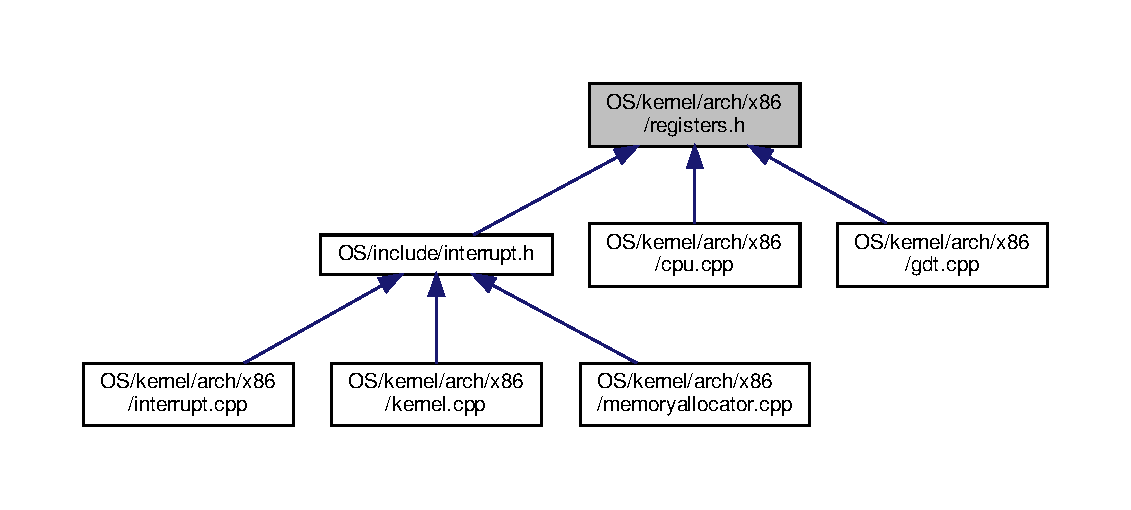
\includegraphics[width=350pt]{registers_8h__dep__incl}
\end{center}
\end{figure}
\subsection*{Namespaces}
\begin{DoxyCompactItemize}
\item 
 \hyperlink{namespace_c_r0}{C\+R0}
\item 
 \hyperlink{namespace_c_r4}{C\+R4}
\item 
 \hyperlink{namespace_f_l_a_g_s}{F\+L\+A\+GS}
\end{DoxyCompactItemize}
\subsection*{Enumerations}
\begin{DoxyCompactItemize}
\item 
enum \+: uint8\+\_\+t \{ \newline
\hyperlink{namespace_c_r0_ad023cbd7e6972678c8d8e7bc35db401aa7f3a9f7cae8ff9783116b3807a9e7f63}{C\+R0\+::\+PE} = 0, 
\hyperlink{namespace_c_r0_ad023cbd7e6972678c8d8e7bc35db401aa5d476977d06d7c0b03c9c15c07a79a67}{C\+R0\+::\+MP} = 1, 
\hyperlink{namespace_c_r0_ad023cbd7e6972678c8d8e7bc35db401aa7b84c2b5b161093766d5ce338ae954fd}{C\+R0\+::\+EM} = 2, 
\hyperlink{namespace_c_r0_ad023cbd7e6972678c8d8e7bc35db401aa11d3ddf6dc3d1d972c1df841c8612a98}{C\+R0\+::\+TS} = 3, 
\newline
\hyperlink{namespace_c_r0_ad023cbd7e6972678c8d8e7bc35db401aaea1442f406aa6dac094cac2466be6da7}{C\+R0\+::\+ET} = 4, 
\hyperlink{namespace_c_r0_ad023cbd7e6972678c8d8e7bc35db401aaec96b199175e3576b8864dc1ac07ac4e}{C\+R0\+::\+NE} = 5, 
\hyperlink{namespace_c_r0_ad023cbd7e6972678c8d8e7bc35db401aa26b870d7f1a47ad83f6c2ce739189171}{C\+R0\+::\+WP} = 16, 
\hyperlink{namespace_c_r0_ad023cbd7e6972678c8d8e7bc35db401aa2325d7d071248d4efffdf7bd809decb7}{C\+R0\+::\+AM} = 18, 
\newline
\hyperlink{namespace_c_r0_ad023cbd7e6972678c8d8e7bc35db401aa09776e60fc989f19ae0f04a402d2d1bb}{C\+R0\+::\+NW} = 29, 
\hyperlink{namespace_c_r0_ad023cbd7e6972678c8d8e7bc35db401aa4154f3b5cb906ec0bfab20c87e8a7d84}{C\+R0\+::\+CD} = 30, 
\hyperlink{namespace_c_r0_ad023cbd7e6972678c8d8e7bc35db401aa674029f08e40b913896b27f5cb5e1ec8}{C\+R0\+::\+PG} = 31
 \}
\item 
enum \+: uint8\+\_\+t \{ \newline
\hyperlink{namespace_c_r4_a8969be482f1ac252e3dc7b9264588f1faa569bc9b3252f731550182a03c650797}{C\+R4\+::\+V\+ME} = 0, 
\hyperlink{namespace_c_r4_a8969be482f1ac252e3dc7b9264588f1fa6b65c8f982880d05c6a32200c60242db}{C\+R4\+::\+P\+VI} = 1, 
\hyperlink{namespace_c_r4_a8969be482f1ac252e3dc7b9264588f1face0ed188ba0369731b44b7df079a518b}{C\+R4\+::\+T\+SD} = 2, 
\hyperlink{namespace_c_r4_a8969be482f1ac252e3dc7b9264588f1fa6ba0a01eeee81d3b2b4165a5084b507a}{C\+R4\+::\+DE} = 3, 
\newline
\hyperlink{namespace_c_r4_a8969be482f1ac252e3dc7b9264588f1faf62a80eb9fee090b45e3962ca9adb6cd}{C\+R4\+::\+P\+SE} = 4, 
\hyperlink{namespace_c_r4_a8969be482f1ac252e3dc7b9264588f1fa3a3afec51c05f51090a3d704d31ff310}{C\+R4\+::\+P\+AE} = 5, 
\hyperlink{namespace_c_r4_a8969be482f1ac252e3dc7b9264588f1fab6bdf44cebbecb78a845af15d91a1d0a}{C\+R4\+::\+M\+CE} = 6, 
\hyperlink{namespace_c_r4_a8969be482f1ac252e3dc7b9264588f1fadef854f9df515146e4f5c5b7c46206ee}{C\+R4\+::\+P\+GE} = 7, 
\newline
\hyperlink{namespace_c_r4_a8969be482f1ac252e3dc7b9264588f1fafd06ff4443c1659425fefcc65fc76419}{C\+R4\+::\+P\+CE} = 8, 
\hyperlink{namespace_c_r4_a8969be482f1ac252e3dc7b9264588f1fab0cf978bb5b8c32070363ab81d327c53}{C\+R4\+::\+O\+S\+F\+X\+SR} = 9, 
\hyperlink{namespace_c_r4_a8969be482f1ac252e3dc7b9264588f1fabb68ec0930317011b84484346947f472}{C\+R4\+::\+O\+S\+X\+M\+M\+E\+X\+C\+PT} = 10
 \}
\item 
enum \+: uint32\+\_\+t \{ \newline
\hyperlink{namespace_f_l_a_g_s_a14e24f40a6d353d39c36f2eb221db9e9a1e61b18dede7337e99c57059e099a7d0}{F\+L\+A\+G\+S\+::\+CF} = 0x0001, 
\hyperlink{namespace_f_l_a_g_s_a14e24f40a6d353d39c36f2eb221db9e9ac2a64b20f171c4a80430f79a148d31d8}{F\+L\+A\+G\+S\+::\+PF} = 0x0004, 
\hyperlink{namespace_f_l_a_g_s_a14e24f40a6d353d39c36f2eb221db9e9abc6c39c7676dd1893ab8cac782962a46}{F\+L\+A\+G\+S\+::\+AF} = 0x0010, 
\hyperlink{namespace_f_l_a_g_s_a14e24f40a6d353d39c36f2eb221db9e9a4ffaf63b236176ba89f7c46efb976922}{F\+L\+A\+G\+S\+::\+ZF} = 0x0040, 
\newline
\hyperlink{namespace_f_l_a_g_s_a14e24f40a6d353d39c36f2eb221db9e9aa824ab195ddb83a9e5a8894457e1e6de}{F\+L\+A\+G\+S\+::\+SF} = 0x0080, 
\hyperlink{namespace_f_l_a_g_s_a14e24f40a6d353d39c36f2eb221db9e9a4fd0673010631e5f1c7597b5157461bc}{F\+L\+A\+G\+S\+::\+TF} = 0x0100, 
\hyperlink{namespace_f_l_a_g_s_a14e24f40a6d353d39c36f2eb221db9e9aec02296c8246d8621db2de2314b6728d}{F\+L\+A\+G\+S\+::\+IF} = 0x0200, 
\hyperlink{namespace_f_l_a_g_s_a14e24f40a6d353d39c36f2eb221db9e9a6d0f5b6510bc2a40631627ef5330fbef}{F\+L\+A\+G\+S\+::\+DF} = 0x0400, 
\newline
\hyperlink{namespace_f_l_a_g_s_a14e24f40a6d353d39c36f2eb221db9e9a10b6a3ccfa73250d20d1b2d5e6f2424f}{F\+L\+A\+G\+S\+::\+OF} = 0x0800, 
\hyperlink{namespace_f_l_a_g_s_a14e24f40a6d353d39c36f2eb221db9e9ab410a125534d3cf535d3be32c134abff}{F\+L\+A\+G\+S\+::\+RF} = 0x0001\textquotesingle{}0000, 
\hyperlink{namespace_f_l_a_g_s_a14e24f40a6d353d39c36f2eb221db9e9a549f5d5262483d77729683894e6d1be0}{F\+L\+A\+G\+S\+::\+VM} = 0x0002\textquotesingle{}0000, 
\hyperlink{namespace_f_l_a_g_s_a14e24f40a6d353d39c36f2eb221db9e9af66a43e8dab676f5753b7abe62a53f62}{F\+L\+A\+G\+S\+::\+AC} = 0x0004\textquotesingle{}0000, 
\newline
\hyperlink{namespace_f_l_a_g_s_a14e24f40a6d353d39c36f2eb221db9e9a60d8e57e033e6621fbda4b775e27ac6a}{F\+L\+A\+G\+S\+::\+V\+IF} = 0x0008\textquotesingle{}0000, 
\hyperlink{namespace_f_l_a_g_s_a14e24f40a6d353d39c36f2eb221db9e9aea811f58ffff15c14f1a3bdb9ec09727}{F\+L\+A\+G\+S\+::\+V\+IP} = 0x0010\textquotesingle{}0000, 
\hyperlink{namespace_f_l_a_g_s_a14e24f40a6d353d39c36f2eb221db9e9a057e038e9149d8fe2ad23df50ef42151}{F\+L\+A\+G\+S\+::\+ID} = 0x0020\textquotesingle{}0000
 \}
\end{DoxyCompactItemize}

\hypertarget{utilities_8cpp}{}\section{O\+S/kernel/arch/x86/utilities.cpp File Reference}
\label{utilities_8cpp}\index{O\+S/kernel/arch/x86/utilities.\+cpp@{O\+S/kernel/arch/x86/utilities.\+cpp}}
{\ttfamily \#include $<$utilities.\+h$>$}\newline
Include dependency graph for utilities.\+cpp\+:
\nopagebreak
\begin{figure}[H]
\begin{center}
\leavevmode
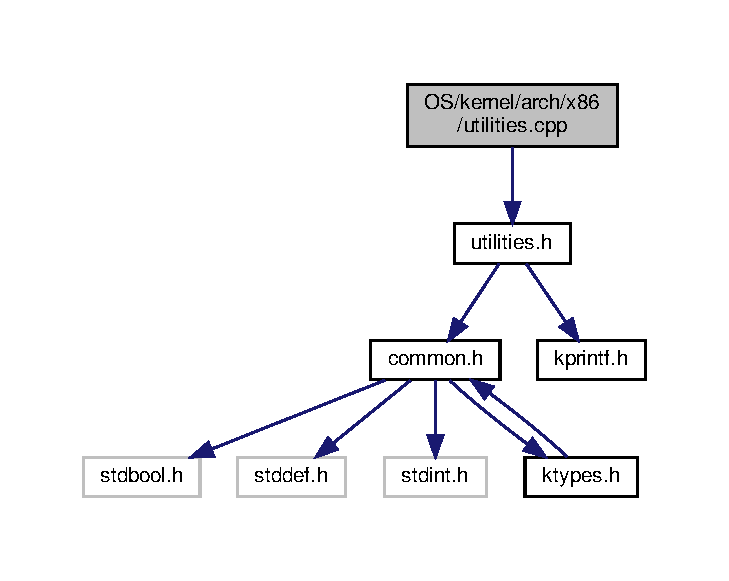
\includegraphics[width=350pt]{utilities_8cpp__incl}
\end{center}
\end{figure}
\subsection*{Functions}
\begin{DoxyCompactItemize}
\item 
size\+\_\+t \hyperlink{utilities_8cpp_a05b27f5e571488d0a74e4bd70b612874}{Strlen} (const char $\ast$Str)
\end{DoxyCompactItemize}


\subsection{Function Documentation}
\mbox{\Hypertarget{utilities_8cpp_a05b27f5e571488d0a74e4bd70b612874}\label{utilities_8cpp_a05b27f5e571488d0a74e4bd70b612874}} 
\index{utilities.\+cpp@{utilities.\+cpp}!Strlen@{Strlen}}
\index{Strlen@{Strlen}!utilities.\+cpp@{utilities.\+cpp}}
\subsubsection{\texorpdfstring{Strlen()}{Strlen()}}
{\footnotesize\ttfamily size\+\_\+t Strlen (\begin{DoxyParamCaption}\item[{const char $\ast$}]{Str }\end{DoxyParamCaption})}



Definition at line 3 of file utilities.\+cpp.


\hypertarget{vga_8cpp}{}\section{O\+S/kernel/arch/x86/vga.cpp File Reference}
\label{vga_8cpp}\index{O\+S/kernel/arch/x86/vga.\+cpp@{O\+S/kernel/arch/x86/vga.\+cpp}}
{\ttfamily \#include $<$vga.\+h$>$}\newline
Include dependency graph for vga.\+cpp\+:
\nopagebreak
\begin{figure}[H]
\begin{center}
\leavevmode
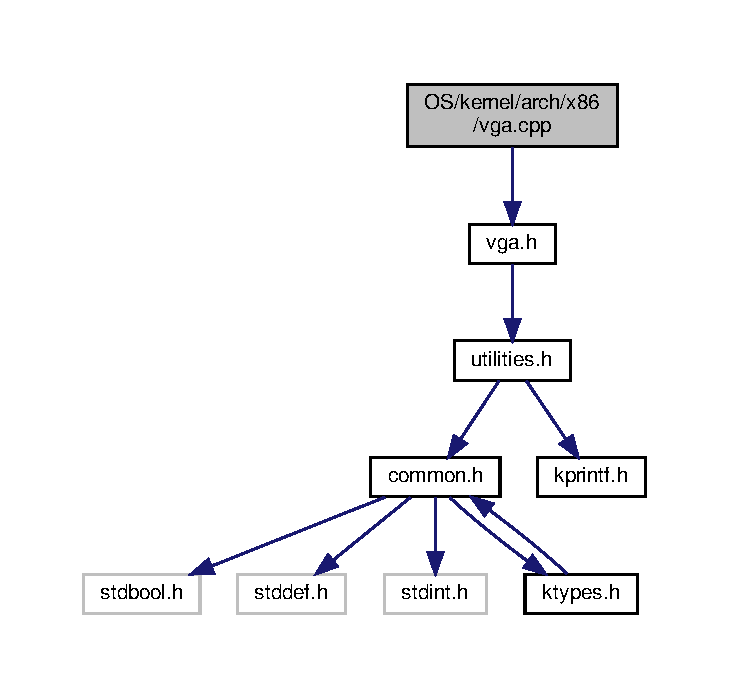
\includegraphics[width=350pt]{vga_8cpp__incl}
\end{center}
\end{figure}
\subsection*{Namespaces}
\begin{DoxyCompactItemize}
\item 
 \hyperlink{namespace_v_g_a}{V\+GA}
\item 
 \hyperlink{namespace_i_n_i_t}{I\+N\+IT}
\end{DoxyCompactItemize}
\subsection*{Functions}
\begin{DoxyCompactItemize}
\item 
void \hyperlink{namespace_i_n_i_t_abae5789d80f8edd37455f3b167779654}{I\+N\+I\+T\+::\+V\+GA} ()
\end{DoxyCompactItemize}

\hypertarget{virtualmemory_8cpp}{}\section{O\+S/kernel/arch/x86/virtualmemory.cpp File Reference}
\label{virtualmemory_8cpp}\index{O\+S/kernel/arch/x86/virtualmemory.\+cpp@{O\+S/kernel/arch/x86/virtualmemory.\+cpp}}
{\ttfamily \#include $<$virtualmemory.\+h$>$}\newline
{\ttfamily \#include $<$registers.\+h$>$}\newline
Include dependency graph for virtualmemory.\+cpp\+:\nopagebreak
\begin{figure}[H]
\begin{center}
\leavevmode
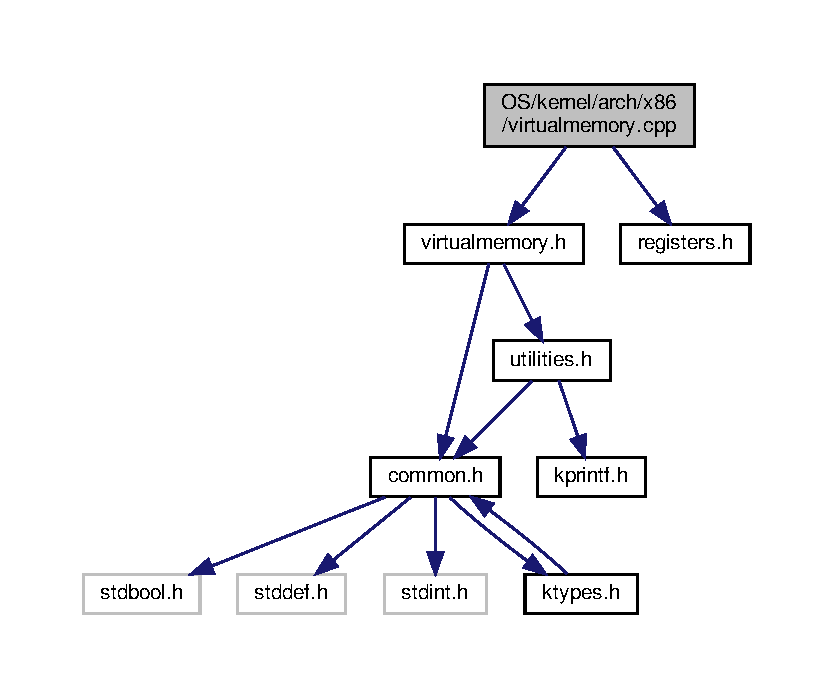
\includegraphics[width=350pt]{virtualmemory_8cpp__incl}
\end{center}
\end{figure}
\subsection*{Namespaces}
\begin{DoxyCompactItemize}
\item 
 \hyperlink{namespace_v_m}{VM}
\begin{DoxyCompactList}\small\item\em Virtual memory namespace. \end{DoxyCompactList}\item 
 \hyperlink{namespace_i_n_i_t}{I\+N\+IT}
\begin{DoxyCompactList}\small\item\em contains all kernel initialization routines \end{DoxyCompactList}\end{DoxyCompactItemize}
\subsection*{Functions}
\begin{DoxyCompactItemize}
\item 
void \hyperlink{namespace_v_m_a722753d2c3fafcd36dad99fb1fa1eaf3}{V\+M\+::\+Initialize\+Page\+Directory} (uint32\+\_\+t Page\+Directory\mbox{[}P\+D\+\_\+\+S\+I\+ZE\mbox{]})
\item 
void \hyperlink{namespace_v_m_a23f571f0afcc986879a5d489ca0a2d4a}{V\+M\+::\+Map\+Page\+Table} (const size\+\_\+t Idx, uint32\+\_\+t Page\+Directory\mbox{[}P\+D\+\_\+\+S\+I\+ZE\mbox{]}, uint32\+\_\+t Page\+Table\mbox{[}P\+T\+\_\+\+S\+I\+ZE\mbox{]})
\begin{DoxyCompactList}\small\item\em Map page table. \end{DoxyCompactList}\item 
void \hyperlink{namespace_v_m_a9c0e1f32f8ec14ae7f246197e5b46498}{V\+M\+::\+Install\+Paging} (const uint32\+\_\+t Page\+Directory\mbox{[}$\,$\mbox{]})
\begin{DoxyCompactList}\small\item\em Set cr3 to page directory, and turn on paging. \end{DoxyCompactList}\item 
void \hyperlink{namespace_i_n_i_t_aea383d3de30095cf9d176fa60b66d01d}{I\+N\+I\+T\+::\+P\+A\+GE} ()
\begin{DoxyCompactList}\small\item\em set up page directory, page table, and turn on paging \end{DoxyCompactList}\end{DoxyCompactItemize}
\subsection*{Variables}
\begin{DoxyCompactItemize}
\item 
void $\ast$ \hyperlink{virtualmemory_8cpp_a6f6f3cc49b2c83f2fc2944156cdca42f}{kpagetable}
\item 
const size\+\_\+t \hyperlink{namespace_v_m_a9a281e32930026b0c172914c1991ee6c}{V\+M\+::\+P\+D\+\_\+\+S\+I\+ZE} = 1024
\begin{DoxyCompactList}\small\item\em page directory size \end{DoxyCompactList}\item 
const size\+\_\+t \hyperlink{namespace_v_m_a64558f9565f1bb4a12eb2ddd7b7c1106}{V\+M\+::\+P\+T\+\_\+\+S\+I\+ZE} = 1024
\begin{DoxyCompactList}\small\item\em page table size \end{DoxyCompactList}\item 
const size\+\_\+t \hyperlink{namespace_v_m_a3afc454e973b965743e84ed10d74161c}{V\+M\+::\+P\+G\+\_\+\+S\+I\+ZE} = 4096
\begin{DoxyCompactList}\small\item\em page size \end{DoxyCompactList}\item 
uint32\+\_\+t \hyperlink{namespace_v_m_a3580800d6decdb1a45fe063c10288201}{V\+M\+::page\+\_\+directory} \mbox{[}P\+D\+\_\+\+S\+I\+ZE\mbox{]}\mbox{[}\mbox{[}gnu\+::aligned(P\+G\+\_\+\+S\+I\+ZE)\mbox{]}\mbox{]}
\item 
uint32\+\_\+t \hyperlink{namespace_v_m_a4b6dc3e8c1df1e3ff30e6585b9da9937}{V\+M\+::pagetable0} \mbox{[}P\+T\+\_\+\+S\+I\+ZE\mbox{]}\mbox{[}\mbox{[}gnu\+::aligned(P\+G\+\_\+\+S\+I\+ZE)\mbox{]}\mbox{]}
\end{DoxyCompactItemize}


\subsection{Variable Documentation}
\mbox{\Hypertarget{virtualmemory_8cpp_a6f6f3cc49b2c83f2fc2944156cdca42f}\label{virtualmemory_8cpp_a6f6f3cc49b2c83f2fc2944156cdca42f}} 
\index{virtualmemory.\+cpp@{virtualmemory.\+cpp}!kpagetable@{kpagetable}}
\index{kpagetable@{kpagetable}!virtualmemory.\+cpp@{virtualmemory.\+cpp}}
\subsubsection{\texorpdfstring{kpagetable}{kpagetable}}
{\footnotesize\ttfamily void$\ast$ kpagetable}



Definition at line 8 of file virtualmemory.\+cpp.


\hypertarget{mainpage_8dox}{}\section{O\+S/mainpage.dox File Reference}
\label{mainpage_8dox}\index{O\+S/mainpage.\+dox@{O\+S/mainpage.\+dox}}

%--- End generated contents ---

% Index
\backmatter
\newpage
\phantomsection
\clearemptydoublepage
\addcontentsline{toc}{chapter}{Index}
\printindex

\end{document}
